% ******************************* PhD Thesis Template **************************
% Please have a look at the README.md file for info on how to use the template

\documentclass[a4paper, 12pt, times, numbered, draft, chapter]{Classes/PhDThesisPSnPDF}

% ******************************************************************************
% ******************************* Class Options ********************************
% *********************** See README for more details **************************
% ******************************************************************************

% `a4paper'(The University of Cambridge PhD thesis guidelines recommends a page
% size a4 - default option) or `a5paper': A5 Paper size is also allowed as per
% the Cambridge University Engineering Deparment guidelines for PhD thesis
%
% `11pt' or `12pt'(default): Font Size 10pt is NOT recommended by the University
% guidelines
%
% `oneside' or `twoside'(default): Printing double side (twoside) or single
% side.
%
% `print': Use `print' for print version with appropriate margins and page
% layout. Leaving the options field blank will activate Online version.
%
% `index': For index at the end of the thesis
%
% `draftclassic': For draft mode without loading any images (same as draft in book)
%
% `draft': Special draft mode with line numbers, images, and water mark with
% timestamp and custom text. Position of the text can also be modified.
%
% `abstract': To generate only the title page and abstract page with
% dissertation title and name, to submit to the Student Registry
%
% `chapter`: This option enables only the specified chapter and it's references
%  Useful for review and corrections.
%
% ************************* Custom Page Margins ********************************
%
% `custommargin`: Use `custommargin' in options to activate custom page margins,
% which can be defined in the preamble.tex. Custom margin will override
% print/online margin setup.
%
% *********************** Choosing the Fonts in Class Options ******************
%
% `times' : Times font with math support. (The Cambridge University guidelines
% recommend using times)
%
% `fourier': Utopia Font with Fourier Math font (Font has to be installed)
%            It's a free font.
%
% `customfont': Use `customfont' option in the document class and load the
% package in the preamble.tex
%
% default or leave empty: `Latin Modern' font will be loaded.
%
% ********************** Choosing the Bibliography style ***********************
%
% `authoryear': For author-year citation eg., Krishna (2013)
%
% `numbered': (Default Option) For numbered and sorted citation e.g., [1,5,2]
%
% `custombib': Define your own bibliography style in the `preamble.tex' file.
%              `\RequirePackage[square, sort, numbers, authoryear]{natbib}'.
%              This can be also used to load biblatex instead of natbib
%              (See Preamble)
%
% **************************** Choosing the Page Style *************************
%
% `default (leave empty)': For Page Numbers in Header (Left Even, Right Odd) and
% Chapter Name in Header (Right Even) and Section Name (Left Odd). Blank Footer.
%
% `PageStyleI': Chapter Name next & Page Number on Even Side (Left Even).
% Section Name & Page Number in Header on Odd Side (Right Odd). Footer is empty.
%
% `PageStyleII': Chapter Name on Even Side (Left Even) in Header. Section Number
% and Section Name in Header on Odd Side (Right Odd). Page numbering in footer

% Uncomment to change page style
%\pagestyle{PageStyleII}

% ********************************** Preamble **********************************
% Preamble: Contains packages and user-defined commands and settings
% ******************************************************************************
% ****************************** Custom Margin *********************************

% Add `custommargin' in the document class options to use this section
% Set {innerside margin / outerside margin / topmargin / bottom margin}  and
% other page dimensions
\ifsetCustomMargin
  \RequirePackage[left=37mm,right=30mm,top=35mm,bottom=30mm]{geometry}
  \setFancyHdr % To apply fancy header after geometry package is loaded
\fi

% Add spaces between paragraphs
%\setlength{\parskip}{0.5em}
% Ragged bottom avoids extra whitespaces between paragraphs
\raggedbottom
% To remove the excess top spacing for enumeration, list and description
%\usepackage{enumitem}
%\setlist[enumerate,itemize,description]{topsep=0em}

% *****************************************************************************
% ******************* Fonts (like different typewriter fonts etc.)*************

% Add `customfont' in the document class option to use this section

\ifsetCustomFont
  % Set your custom font here and use `customfont' in options. Leave empty to
  % load computer modern font (default LaTeX font).
  %\RequirePackage{helvet}

  % For use with XeLaTeX
  %  \setmainfont[
  %    Path              = ./libertine/opentype/,
  %    Extension         = .otf,
  %    UprightFont = LinLibertine_R,
  %    BoldFont = LinLibertine_RZ, % Linux Libertine O Regular Semibold
  %    ItalicFont = LinLibertine_RI,
  %    BoldItalicFont = LinLibertine_RZI, % Linux Libertine O Regular Semibold Italic
  %  ]
  %  {libertine}
  %  % load font from system font
  %  \newfontfamily\libertinesystemfont{Linux Libertine O}
\fi

% *****************************************************************************
% **************************** Custom Packages ********************************

% ************************* Algorithms and Pseudocode **************************

%\usepackage{algpseudocode}


% ********************Captions and Hyperreferencing / URL **********************

% Captions: This makes captions of figures use a boldfaced small font.
%\RequirePackage[small,bf]{caption}

\RequirePackage[labelsep=space,tableposition=top]{caption}
\renewcommand{\figurename}{Fig.} %to support older versions of captions.sty


% *************************** Graphics and figures *****************************

%\usepackage{rotating}
%\usepackage{wrapfig}

% Uncomment the following two lines to force Latex to place the figure.
% Use [H] when including graphics. Note 'H' instead of 'h'
%\usepackage{float}
%\restylefloat{figure}

% Subcaption package is also available in the sty folder you can use that by
% uncommenting the following line
% This is for people stuck with older versions of texlive
%\usepackage{sty/caption/subcaption}
\usepackage{subcaption}

% ********************************** Tables ************************************
\usepackage{booktabs} % For professional looking tables
\usepackage{multirow}

%\usepackage{multicol}
%\usepackage{longtable}
%\usepackage{tabularx}


% *********************************** SI Units *********************************
\usepackage{siunitx} % use this package module for SI units


% ******************************* Line Spacing *********************************

% Choose linespacing as appropriate. Default is one-half line spacing as per the
% University guidelines

% \doublespacing
% \onehalfspacing
% \singlespacing


% ************************ Formatting / Footnote *******************************

% Don't break enumeration (etc.) across pages in an ugly manner (default 10000)
%\clubpenalty=500
%\widowpenalty=500

%\usepackage[perpage]{footmisc} %Range of footnote options


% *****************************************************************************
% *************************** Bibliography  and References ********************

%\usepackage{cleveref} %Referencing without need to explicitly state fig /table

% Add `custombib' in the document class option to use this section
\ifuseCustomBib
   \RequirePackage[square, sort, numbers, authoryear]{natbib} % CustomBib

% If you would like to use biblatex for your reference management, as opposed to the default `natbibpackage` pass the option `custombib` in the document class. Comment out the previous line to make sure you don't load the natbib package. Uncomment the following lines and specify the location of references.bib file

%\RequirePackage[backend=biber, style=numeric-comp, citestyle=numeric, sorting=nty, natbib=true]{biblatex}
%\bibliography{References/references} %Location of references.bib only for biblatex

\fi

% changes the default name `Bibliography` -> `References'
\renewcommand{\bibname}{References}


% ******************************************************************************
% ************************* User Defined Commands ******************************
% ******************************************************************************

% *********** To change the name of Table of Contents / LOF and LOT ************

%\renewcommand{\contentsname}{My Table of Contents}
%\renewcommand{\listfigurename}{My List of Figures}
%\renewcommand{\listtablename}{My List of Tables}


% ********************** TOC depth and numbering depth *************************

\setcounter{secnumdepth}{2}
\setcounter{tocdepth}{2}


% ******************************* Nomenclature *********************************

% To change the name of the Nomenclature section, uncomment the following line

%\renewcommand{\nomname}{Symbols}


% ********************************* Appendix ***********************************

% The default value of both \appendixtocname and \appendixpagename is `Appendices'. These names can all be changed via:

%\renewcommand{\appendixtocname}{List of appendices}
%\renewcommand{\appendixname}{Appndx}

% *********************** Configure Draft Mode **********************************

% Uncomment to disable figures in `draft'
%\setkeys{Gin}{draft=true}  % set draft to false to enable figures in `draft'

% These options are active only during the draft mode
% Default text is "Draft"
%\SetDraftText{DRAFT}

% Default Watermark location is top. Location (top/bottom)
%\SetDraftWMPosition{bottom}

% Draft Version - default is v1.0
%\SetDraftVersion{v1.1}

% Draft Text grayscale value (should be between 0-black and 1-white)
% Default value is 0.75
%\SetDraftGrayScale{0.8}


% ******************************** Todo Notes **********************************
%% Uncomment the following lines to have todonotes.

%\ifsetDraft
%	\usepackage[colorinlistoftodos]{todonotes}
%	\newcommand{\mynote}[1]{\todo[author=kks32,size=\small,inline,color=green!40]{#1}}
%\else
%	\newcommand{\mynote}[1]{}
%	\newcommand{\listoftodos}{}
%\fi

% Example todo: \mynote{Hey! I have a note}

% ************************ Thesis Information & Meta-data **********************
% Thesis title and author information, refernce file for biblatex
% ************************ Thesis Information & Meta-data **********************
%% The title of the thesis
\title{Accelerating the Design-Make-Test cycle of Drug Discovery with Machine Learning}
%\texorpdfstring is used for PDF metadata. Usage:
%\texorpdfstring{LaTeX_Version}{PDF Version (non-latex)} eg.,
%\texorpdfstring{$sigma$}{sigma}

%% Subtitle (Optional)
% \subtitle{that actually works}

%% The full name of the author
\author{William McCorkindale}

%% Department (eg. Department of Engineering, Maths, Physics)
\dept{Cavendish Laboratory, Department of Physics}

%% University and Crest
\university{University of Cambridge}
% Crest minimum should be 30mm.
\crest{
\includegraphics[width=0.2\textwidth]{University_Crest}}
%% Use this crest, if you are using the college crest
%% Crest long miminum should be 65mm
%\crest{
\includegraphics[width=0.45\textwidth]{University_Crest_Long}}

%% College shield [optional] 
% Crest minimum should be 30mm.
%\collegeshield{
\includegraphics[width=0.2\textwidth]{CollegeShields/Kings}}


%% Supervisor (optional)
%% for multiple supervisors, append each supervisor with the \newline command
\supervisor{Dr. Alpha Lee}

%% Supervisor Role (optional) - Supervisor (default) or advisor
% \supervisorrole{\textbf{Supervisors: }}
%% if no title is desired:
% \supervisorrole{}

%% Supervisor line width: required to align supervisors
% \supervisorlinewidth{0.35\textwidth}

%% Advisor (optional)
%% for multiple advisors, append each advisor with the \newline command
%\advisor{Dr. A. Advisor\newline
%Dr. B. Advisor}
     
%% Advisor Role (optional) - Advisor (default) or leave empty
% \advisorrole{Advisors: }
%% if no title is required
% \advisorrole{}

%% Advisor line width: required to align supervisors
%\advisorlinewidth{0.25\textwidth}


%% You can redefine the submission text:
% Default as per the University guidelines:
% ``This dissertation is submitted for the degree of''
\renewcommand{\submissiontext}{}

%% Full title of the Degree
% \degreetitle{Doctor of Philosophy}

%% College affiliation (optional)
\college{St. John's College}

%% Submission date
% Default is set as {\monthname[\the\month]\space\the\year}
%\degreedate{September 2014} 

%% Meta information
\subject{LaTeX} \keywords{{LaTeX} {PhD Thesis} {Physics} {University of
Cambridge}}


% ***************************** Abstract Separate ******************************
% To printout only the titlepage and the abstract with the PhD title and the
% author name for submission to the Student Registry, use the `abstract' option in
% the document class.

\ifdefineAbstract
 \pagestyle{empty}
 \includeonly{Declaration/declaration, Abstract/abstract}
\fi

% ***************************** Chapter Mode ***********************************
% The chapter mode allows user to only print particular chapters with references
% Title, Contents, Frontmatter are disabled by default
% Useful option to review a particular chapter or to send it to supervisior.
% To use choose `chapter' option in the document class

\ifdefineChapter
 	% \includeonly{Chapters/Preface/preface}
 	\includeonly{Chapters/Background/background}
 	% \includeonly{Chapters/Ranking/ranking}
%  	\includeonly{Chapters/Fresco/fresco}
 	% \includeonly{Chapters/Transformer/transformer}
 	% \includeonly{Chapters/Crude/test}

\fi

% ******************************** Front Matter ********************************
\begin{document}

\frontmatter

\maketitle

% % ******************************* Thesis Dedication ********************************

\begin{dedication} 

I would like to dedicate this thesis to my loving parents \dots

First and foremost, I would like to sincerely thank my advisor Alpha Lee for his help, guidance and for the freedom I was granted throughout these years.

In alphabetical order, I would also like to thank my colleagues who \dots: Dávid, Emma, Felix,  Janosh, Kadi, Penny, Rokas, Rhys.

David, Michelle, Brian. Gates scholars. CUHKPGSA?

I would finally like to warmly thank my dear housemates Dávid and Eszti for their help in moments of doubt.

WM acknowledges the support of the Gates Cambridge Trust.

\end{dedication}
% ******************************* Thesis Declaration ***************************

\begin{declaration}

I hereby declare that except where specific reference is made to the work of others, the contents of this dissertation are original and have not been submitted in whole or in part for consideration for any other degree or qualification in this, or any other university. This dissertation is my own work and contains nothing which is the outcome of work done in collaboration with others, except as specified in the Preface and Acknowledgements. This  dissertation contains fewer than 65,000 words including appendices,  bibliography, footnotes, tables and equations and has fewer than 150 figures.

The research described in this thesis was performed between October 2019 and December 2022, and was supervised by Dr Alpha A. Lee.
% Author and date will be inserted automatically from thesis.tex \author \degreedate

\end{declaration}
% ************************** Thesis Acknowledgements **************************

\begin{acknowledgements}

TODO - finish acknowledgements

First and foremost, I would like to sincerely thank my supervisor Dr Alpha A. Lee for his invaluable guidance, support, and encouragement throughout my PhD journey. I am deeply grateful for his commitment to my success and for his role in shaping my personal and professional development.

In alphabetical order, I would also like to thank my colleagues in the Lee Group: Dávid, Emma, Felix, Janosh, Kadi, Penny, Rokas, Rhys. Their knowledge, expertise, and friendship have been invaluable in shaping my research and personal growth. I feel very fortunate to have had the opportunity to work with and learn from you all, and I will always cherish the memories and lessons learned from our time together.

I was generously funded by the Gates Cambridge Scholarship to undertake this research, and I am very grateful for their support, as well as for the many friendships I have made in the Gates scholar community. I would like to give special thanks in particular to David and Michelle, for their friendship and support.

Friends from Cambridge. Brian.

Upheaval in my birthplace, Hong Kong. CUHKPGSA

Much of the research in this thesis was conducted during the COVID-19 pandemic, when I spent a considerable amount of time indoors with my dear housemates Dávid and Eszti. I will be forever grateful for their unwavering friendship, humor, and kindness during some of the most challenging times of my PhD journey.

I would like to thank Marika for always putting a smile on my face and reminding me what is truly important in life.

Lastly, I would like to thank my parents, John and Maureen, for their unconditional love and continual support.

\end{acknowledgements}

% ************************** Thesis Abstract *****************************
% Use `abstract' as an option in the document class to print only the titlepage and the abstract.
\begin{abstract}
Drug discovery follows a design-make-test cycle of proposing drug compounds, synthesising them, and measuring their bioactivity, which informs the next cycle of compound designs. The challenges associated with each step leads to the long timeline of preclinical pharmaceutical development. This thesis focuses on how we can use machine learning tools to accelerate the design-make-test cycle for faster drug discovery.

We begin with the design of new compounds, looking at the initial stage of fragment-based hit finding where only the 3D coordinates of fragment-protein complexes are available. The standard approach is to “grow” or “merge” nearby fragments based on their binding modes, but fragments typically have low affinity so the road to potency is often long and fraught with false starts. Instead, we can reframe fragment-based hit discovery as a denoising problem - identifying significant pharmacophore distributions from an “ensemble” of fragments amid noise due to weak binders - and employ an unsupervised machine learning method to tackle this problem. We construct a model that screens potential molecules by evaluating whether they recapitulate those fragment-derived pharmacophore distributions. We show that this approach outperforms docking on distinguishing active compounds from inactive ones on historical data. Further, we prospectively find novel hits for SARS-CoV-2 Mpro and the Mac1 domain of SARS-CoV-2 non-structural protein 3 by screening a library of 1B molecules.

After identifying hit compounds, we enter the the hit-to-lead stage where we wish to optimise their molecular structures to improve bioactivity. Framing bioactivity modelling as classification of active/inactive would not allow us to rank compounds based on predicted bioactivity improvement, while the low number of active compounds and the measurement noise make a regression approach challenging. We overcome this challenge with a learning-to-rank framework via a classifier that predicts whether a compound is more or less active than another using the difference in molecular descriptors between the molecules as input. This allows us to make use of inactive data, and threshold the bioactivity differences above measurement noise. Validation on retrospective data for Mpro shows that we can outperform docking on ranking ligands, and we prospectively screen a library of 8.8M molecules and arrive at a potent compound with a novel scaffold.

After designing a drug candidate one needs to find a synthesis route to actually make the molecule in the real world. An exciting approach is to use deep learning models trained on patent reaction databases, but they suffer from being opaque black-boxes. It is neither clear if the models are making correct predictions because they inferred the salient chemistry, nor is it clear which training data they are relying on to reach a prediction. To address this issue, we developed a workflow for quantitatively interpreting a state-of-the-art deep learning model for reaction prediction. By analysing chemically selective reactions, we show examples of correct reasoning by the model, explain counterintuitive predictions, and identify Clever Hans predictions where the correct answer is reached for the wrong reason due to dataset bias.

Testing a drug candidate typically involves obtaining a pure sample of the molecule, and then measuring its bioactivity in solution via an assay. While necessary for maximum accuracy, compound purification can be time-consuming and costly. We investigated whether we needed compound purification at all for training machine learning bioactivity models by assaying crude reaction mixtures instead of pure samples. This approach allowed us to obtain bioactivity data in higher throughput and train useful models for identification of false negative assay measurements, as well as prospective screens.

The research presented in this thesis highlights the promise of applying machine learning in accelerating the design-make-test cycle of drug discovery. This thesis concludes by outlining promising research directions for applying machine learning within drug discovery.
\end{abstract}


% *********************** Adding TOC and List of Figures ***********************

\tableofcontents

% \listoffigures

% \listoftables

% \printnomenclature[space] space can be set as 2em between symbol and description
%\printnomenclature[3em]

% \printnomenclature

% ******************************** Main Matter *********************************
\mainmatter

% TODO - update chapter names
\chapter*{Preface}
\addcontentsline{toc}{chapter}{Preface}
\hyperref[ch:intro]{Chapter 1} introduces the design-make-test cycle in drug discovery and the promise of machine learning (ML) for accelerating the process.

\hyperref[ch:background]{Chapter 2} gives an overview of molecular featurisation and computational methods which are used in this thesis. COVID Moonshot, a drug discovery inititative that much of this thesis is based on, is also introduced.

In \hyperref[ch:fresco]{Chapter 3} starts at the hit-finding stage of drug discovery, and we discuss the usage of unsupervised learning for modelling the 3D distribution of pharmacophores in fragment-protein complexes. This work resulted in the following preprint (manuscript under review):
\begin{quote}
William McCorkindale, Ivan Ahel, Haim Barr, Galen J. Correy, James S. Fraser, Nir London, Marion Schuller, Khriesto Shurrush, Alpha A. Lee. Fragment-Based Hit Discovery via Unsupervised Learning of Fragment-Protein Complexes.
\end{quote}
In this work, I implemented the model and conducted the computational validation and virtual screening. Dr Ivan Ahel, Dr Haim Barr, Dr Khriesto Shurrush, and Prof Nir London performed bioactivity assays of ligands against SARS-CoV-2 Mpro. Dr Galen Correy and Prof James Fraser obtained X-ray crystallographic structures of ligand-bound structures to SARS-CoV-2 nsp3-Mac1. Dr Marion Schuller performed bioactivity assays of ligands against nsp3-Mac1. Dr Alpha A. Lee supervised the work.

\hyperref[ch:ranking]{Chapter 4} brings us to the hit-to-lead stage where modelling bioactivity becomes possible, and we discuss using a model that learns to rank molecules pairwise by activity. This work resulted in the following publication:
\begin{quote}
Aaron Morris, William McCorkindale, The COVID Moonshot Consortium, Nir Drayman, John D. Chodera, Savaş Tay, Nir London, and Alpha A. Lee. Discovery of SARS-CoV-2 main protease inhibitors using a synthesis-directed de novo design model, \textit{Chem. Commun.}, 2021,57, 5909-5912 
\end{quote}
In this work, I developed the ranking model and constructed the screening library. Aaron Morris evaluated the model and generated compound synthesis routes. Dr John D. Chodera performed docking calculations. Prof Nir London performed bioactivity assays of ligands against SARS-CoV-2 Mpro. Dr Nir Drayman and Prof Savaş Tay performed OC43 live virus assays. Dr Alpha A. Lee supervised the work.

In \hyperref[ch:transformer]{Chapter 5} we quantitatively explain predictions from deep learning models used for chemical reactions prediction, revealing model biases due to shortcomings in the training data. This work resulted in the following publication:
\begin{quote}
Dávid Péter Kovács, William McCorkindale and Alpha A. Lee. Quantitative interpretation explains machine learning models for chemical reaction prediction and uncovers bias. \textit{Nature Communications} volume 12, Article number: 1695 (2021)
\end{quote}
I worked jointly with Dávid Kovács on this work which he completed as part of his MPhil research project under Dr Alpha A. Lee. We contributed equally to model development. Dávid Kovács trained the models and analysed the model attributions for various reaction classes. I applied reaction templates for data analysis and artificial dataset generation and investigated model performance under Tanimoto splitting. Dr Alpha A. Lee supervised the work.

\hyperref[ch:testing]{Chapter 6} discusses the training of ML models on high-throughput bioactivity measurements from crude reaction mixtures instead of purified compounds. This research was carried out in collaboration with Dr Emma King-Smith, Mihajlo Filep, Prof Nir London, and Dr Alpha A. Lee. In this work, I implemented the random forest model and constructed the screening library. Dr Emma King-Smith implemented the gaussian process model and cleaned the experimental data. Mihajlo Filep performed bioactivity assays against SARS-CoV-2 Mpro. Dr Alpha A. Lee and Prof Nir London supervised the work.

The final chapter summarises the research presented and discusses promising directions for future research.

During the course of this thesis, several fruitful collaborations have also led to the following publications. These are not discussed in detail within this dissertation.

\begin{quote}
 Kadi L. Saar, William McCorkindale, Daren Fearon, Melissa Boby, Haim Barr, Amir Ben-Shmuel, The COVID Moonshot Consortium, Nir London, Frank von Delft, John D. Chodera and Alpha A. Lee. Turning high-throughput structural biology into predictive inhibitor design. \textit{Proceedings of the National Academy of Sciences} volume 120 (11), Article number: e2214168120 (2023)
\end{quote}

\begin{quote}
 Ryan-Rhys Griffiths, Jake L Greenfield, Aditya R Thawani, Arian R Jamasb, Henry B Moss, Anthony Bourached, Penelope Jones, William McCorkindale, Alexander A Aldrick, Matthew J Fuchter, and Alpha A. Lee. Data-driven discovery of molecular photoswitches with multioutput Gaussian processes. \textit{Chemical Science} volume 13 (45), Article number: 13541-13551 (2022)
\end{quote}
\chapter{Introduction} \label{ch:intro}

The design of a new pharmaceutical treatment for a disease is a complex process involving many stages. Breakthroughs in medical research have enabled a wide variety of different treatment modailities ranging from vaccines to gene therapy, tailored for different diseases - in this thesis, we will narrow our scope to small-molecule drugs, which remain the most common form of treatment for a wide variety of diseases. The development of a new small molecule drug begins with the identification of a target, which is a protein or other biomolecule that plays a role in the disease's biochemical mechanism of action. Afterwards a `hit' compound, which is a small molecule that binds to the target with relatively weak potency, is found as the starting point for a drug design campaign. This brings us to the `hit-to-lead' stage where modifications to the hit are performed to identify a lead compound, which is a small molecule that is potent against the target at very low concentrations. The lead is then optimized to improve its other molecular properties such as target selectivity, solubility, and toxicity. Finally, the lead is taken into preclinical studies and clinical trials to determine its safety and efficacy in humans.

The stages between target identification and preclinical study traditionally follow the design-make-test paradigm, where molecules are repeatedly proposed, synthesized, and assayed. Drug candidates are designed based on some hypothesis relating chemical structure to bioactivity/molecular properties, which gets updated in light of new activity results. This cycle repeats as the molecular search space narrows down until a candidate molecule satisfies the necessary bioactivity/selectivity/toxicity criteria.

The time taken to fully complete a drug design campaign from target identification to preclinical studies can be very time-consuming, costly and there is always a risk of failure if an inappropriate target is chosen or unanticipated side effects are revealed during clinical trials due to the complexity of biology. The costs of developing a new drug have been increasing over time for a multitude of reasons, and there is a pressing need to reduce the time and cost of the drug discovery process.

\begin{figure}[!h] % !h ~ force here, t ~ top, b ~ bottom, p ~ separate page
    \centering
    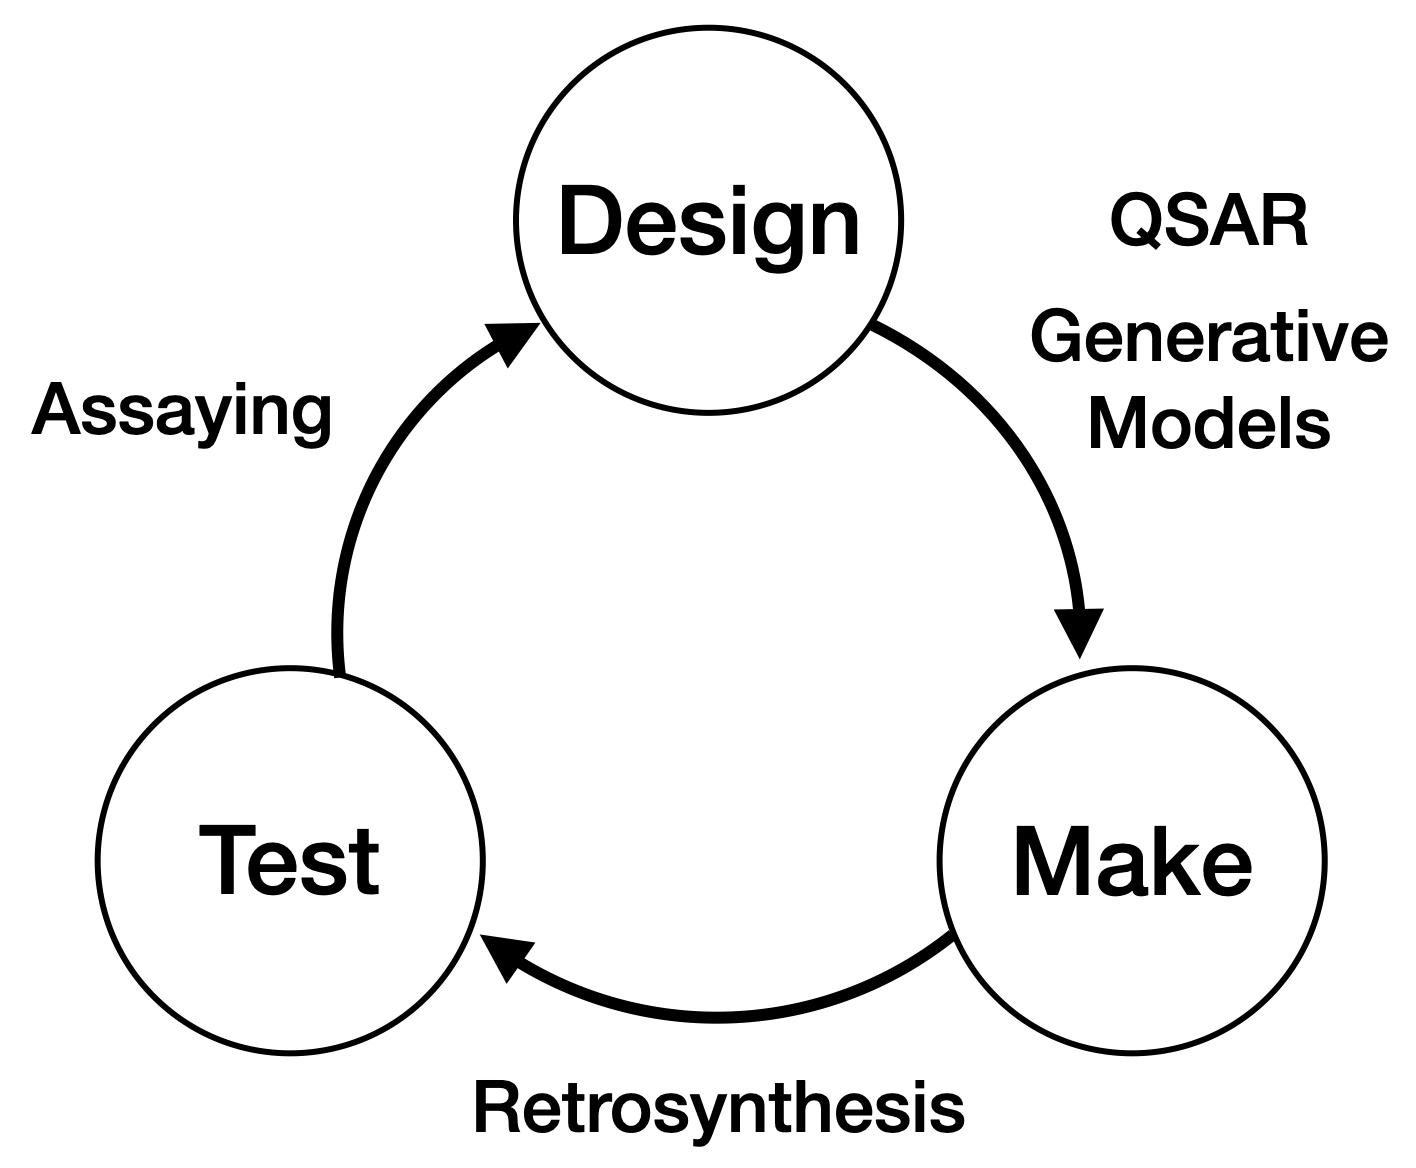
\includegraphics[width=0.5\textwidth]{Chapters/Intro/Figs/design-make-test.png}
    \caption{\label{fig:cycle} An overview of the design-make-test cycle in drug discovery.}
\end{figure}

Computational methods offer a promising avenue to accelerate the drug discovery process by automating the design-make-test cycle. The dream of replacing slow and expensive experiments with fast and cheap predictive algorithms is not a new one, and continuous progress has been made in this direction over the past few decades. Recently, there has been a huge surge in applying machine learning (ML) methods to drug design following its success in various other fields, most notably computer vision and natural language processing.

The application focus for these ML methods have been on the `design' and `make' parts of the cycle, where they have outperformed traditional approaches on a variety of tasks from property prediction to synthesis route planning, and efforts are underway to use ML models to replace aspects of decision-making conventionally done by humans, such as the design of drug candidates.

Much of the progress in this area comes from adapting the latest state-of-the-art algorithms from the ML literature, and while this is a good starting point, it is not sufficient to fully leverage the potential of ML in drug discovery. The quantity and structure of data that is available in drug discovery is very different from that conventionally found in ML applications, and it is necessary to confront this fact and tailor ML models specifically for the unique problems and situations faced in pharmaceutical chemistry in order to drive the development of computational tools that truly suit our needs for accelerating the drug discovery process.

This is the key challenge that we shall explore in this thesis - how we can leverage data-driven approaches based on machine learning in the design-make-test cycle, grappling with the practical difficulties of a drug discovery campaign where we must make full use of the limited data available.

\section*{Design}

The `Design' stage can be broken down into two challenges: (i) predicting the property of a compound from its structure, and (ii) using that predictive model to propose a set of new compounds that are likely to have the desired property. The first challenge has historically been very well-studied: As stated by Alexander Crum Brown in 1868, the ``physiological response of a compound is merely a function of its chemical constitution'' \cite{Brown1868} - chemists have been endeavoring to define this function and predict the properties of compounds without synthesizing them since.

A milestone in the field was made by Hansch and Frujita in 1962 in defining Quantitative Structure-Activity Relationship (QSAR) equations. These were manually defined mathematical models that could be used to predict molecular properties such as the octanol/water partition coefficient (logP) and biological activity, from descriptor coeffiecients derived from molecular structure \cite{hansch1962correlation, hansch1964p}.

Coincidentally, the field of artificial intelligence (AI) was also born in the late 1950s/1960s and the potential of applying computational methods to chemistry was recognized early on with the Dendral system in 1965, which assisted chemists in interpreting mass spectrometry data \cite{Lindsay1993Dendral}. Dendral is not only recognised as the first formal application of AI to chemistry, but also as the first expert system since it was capable of automating some tasks of organic chemists, such as problem solving and thereby improving decision making.

Further research into applying AI in chemistry greatly decreased following the general collapse in AI research from the 1970s onwards, and afterwards the workhorse for computational methods in drug design has been in the use of simulations. Advances in computational processing power and the availability of protein-ligand crystal structures led to the development and use of techniques such as molecular docking, molecular dynamics, and free energy perturbation (FEP) \cite{Yu2017CADDMethods}. The success of these methods have cemented the role of computational tools in drug discovery, and they remain in extensive use today.

The breakthoughs of machine learning in other fields such as image recognition and natural language processing in the 21st century has led to a resurgence of interest in applying these methods to drug discovery. The victory of a nerual network model in the Merck molecular activity challenge \cite{Ma2015MerckMolecularActivity} set in motion active research into the application of deep learning for molecular property prediction which continues to this day.

Much of this research consists of translating the latest state-of-the-art algorithms from the ML literature and applying them to the same retrospective QSAR model benchmarks repeatedly to compare performance between different models. While this has undeniable value in quantitatively driving the development of improved models, by focusing only on retrospective benchmarks and avoiding prospective deployment, model developers overlook the unique challenges faced in real-world drug discovery and the practical needs of the end user \cite{Kearnes2021Prospective}.

This thesis addresses this in two places. In Chapter \ref{ch:fresco} we look at how to leverage fragment-protein structures from a crystallographic fragment screen to perform hit discovery in the absence of any bioactivity data via an unsupervised learning approach. Moving onwards to the early hit-to-lead stage, where bioactivity data is limited, noisy, and dominated by inactive molecules, in Chapter \ref{ch:ranking} we use a learning-to-rank framework to make use of inactive data and overcome experimental noise.

Once a predictive model is obtained, the next step of `Design' is to propose a set of new compounds for synthesis and testing. Traditionally this is done by applying the predictive model on a library of compounds (either commercially available or constructed by human experts), and selecting the top scoring compounds. However, this approach is limited by the coverage of the library, and vast chemical space remains unexplored. Generative deep learning models have been proposed as an alternative approach, where a neural network that can generate novel compounds is combined with a predictive model for exploring chemical space. This approach has shown to be successful for several toy problems and offer an interesting alternative to traditional library screening, particularly in the context of intellectual property \cite{Meyers2021DeNovo}. However, even for toy examples it has been shown that imperfections in the predictive model are exploited by the generative model to generate flawed compounds \cite{Renz2019FailureModes}. This is a problem that will be exacerbated in a real world use case, and it is clear that improving predictive modelling of molecular properties is the fundamental bottleneck to successful `Design'.

\section*{Make}
After proposing a set of compounds, the next step is to synthesize them - the central focus of the field of synthetic organic chemistry. Designing a set of chemical reactions that transform a set of starting materials into a target molecule is approached via retrosynthetic analysis, a concept introduced by E.J. Corey \cite{corey1991logic}. In this approach, the target molecule is progressively simplified into  precursor molecules until commercially available compounds are reached. This logical approach paved the way for the successful synthesis of many complex molecules, for which Corey was awarded the Nobel Prize in Chemistry in 1990 \cite{NobelCorey}.

In addition to introducing the concept of retrosynthetic analysis, Corey was also a pioneer in applying computational methods to support the design of synthetic routes \cite{Corey1985ComputerAssistedSynthesis}. By utilising computers to search databases of available compounds as well as previously recorded chemical reactions instead of relying on the necessarily limited experience and domain knowledge of individual chemists, computational tools allowed the design of shorter, more efficient synthesis routes.

Modern-day approaches build on this work, employing deep learning models instead. By taking advantage of vast repostiories of reaction data held in public and propreitary databases as well as ever-growing libraries of commercially available building blocks, ML models for synthesis planning have found significant success in determining synthetic tractability as well as synthesis planning \cite{Coley2018}. Indeed, recent state-of-the-art models have demonstrated their effectiveness through a variation of the Turing test, where computationally designed synthesis routes compete well against those from expert human organic chemists \cite{Coley19WLDN5}.

While there remain limitations on predicting subtle selectivities and reaction yields, it is generally accepted that ML models can accurately predict the major products of reactions that are well-represented in public datasets. This has led to their increasing deployment and use in industry.

However, deep learning-based reaction prediction models critically suffer from a lack of interpretability. Their black-box nature means it is neither clear if the models are making correct predictions because of correct reasoning, nor is it clear what training data and biases they are relying on to reach a prediction \cite{Jimenze2020XAI}. As these models are made more and more available to non-expert end users, it is increasingly important to understand the decision-making of these models in order to avoid incorrect predictions and drive the development of more robust models. To address this, in Chapter \ref{ch:transformer} we showcase a workflow for explaining the reasoning of reaction prediction models.

\section*{Test}
The major focus of machine learning approaches to property prediction has been on improving performance on retrospective datasets, typically involving curated biological activity data obtained from biochemical assays. A great deal of effort is spent on improving molecular representation and the predictive performance of these models, but relatively little thought is given on how this experimental data is generated, and the Test step of the drug discovery process is largely treated as a black box. 

In reality, different biochemical assay techniques have different accuracies and idiosyncracies and the data generated from different assays should not be modelled equally \cite{Hughes2011Principles}. Innovative experimental techniques such as phenotype screening \cite{Chandrasekaran2021Phenotype}, DNA-/Peptide-encoded libraries \cite{GirondaMartinez2021DNALibrary, Rossler2023PeptideLibrary}, and high-throughput spectrometry \cite{Dunas2023MassSpec} are being developed and there are exciting opportunities to apply machine learning methods for the interpretation of these new forms of experimental data.

Beyond just developing ML models to learn this kind of data, there is great potential in engaging with experimentalists to more tightly integrate ML with experimental techniques for the design of ML-centric design-make-test workflows. We explore this in Chapter \ref{ch:testing} where we apply machine learning on crude bioactivity data from nanomolar-scale high-thoughput chemistry.

\chapter{Molecular Representations and Computational Methods in Drug Discovery} \label{ch:background}

\section{Molecular Representation}

\subsection{SMILES}
The simplified molecular-input line-entry system (SMILES) \cite{Weininger1988, Weininger1989} is a widely-used text-based description of molecular structure. In SMILES strings, atoms are represented with their chemical symbols and aromatic atoms are denoted in lowercase (see Table~\ref{table:smiles} for examples). Single and aromatic bonds are omitted while for double and triple bonds the specials characters \texttt{=} and \texttt{\#} are used. Branches are specified by enclosing them into parentheses. To encode cyclic structures a single bond in the ring is broken and the matching atoms are denoted by numbers. \texttt{@} characters are used to denote chirality while \texttt{\textbackslash} and \texttt{/} characters specify local double bond configurations. Following these rules, a SMILES string is constructed by traversing the nodes of the molecular graph. Depending on the choice of starting node and traversal route there are often multiple valid SMILES representations per molecule, especially for larger molecules. In order to define a single unique SMILES representation for a molecule, known as the `canonical' SMILES, a deterministic algorithm is used to choose the starting node and traversal route.

\begin{table}[!h]
\begin{center}
    \begin{tabular}{|c|c|}
    \hline
         SMILES & Structure \\
         \hline
         C & CH\textsubscript{4} \\
         \lbrack Fe2+\rbrack & Fe\textsuperscript{2+} \\
         C=O & CH\textsubscript{2}O \\
         C\#N & HCN (cyan) \\
         CCN(CC)CC & 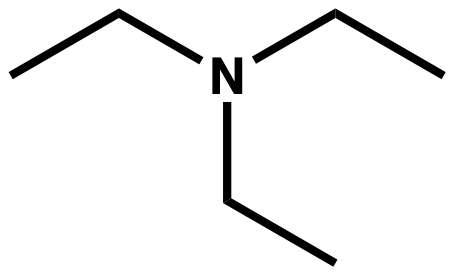
\includegraphics[width=0.75in]{Chapters/Background/Figs/triethyl_amine.png} \\
         CC1=CC(CCC1)Br & 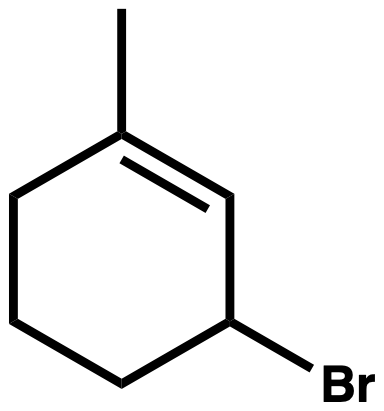
\includegraphics[width=0.7in]{Chapters/Background/Figs/cyclic.png} \\
         \hline
    \end{tabular}
    \caption{Demonstration of the SMILES language}
    \label{table:smiles}
\end{center}
\end{table}

Reaction SMILES are a simple extension of SMILES for specifying chemical reactions. Reaction SMILES strings constructed by placing a \texttt{>} character between the SMILES strings of reactants, reagents, and products. If multiple molecules participate in the reactio, their SMILES strings are separated by a period (\texttt{.}) character.

The text-based nature of SMILES strings as well as its expressiveness in encoding the molecular graph alongside stereochemistry results in its widespread use for storing chemical data. In the context of machine learning, the vast majority of molecular datasets where ML models are used will have molecules represented as SMILES strings. For example, the ESOL dataset consists of 1128 SMILES strings alongside the measured solubility value for each molecule \cite{delauney2004esol}, while USPTO consists of ~480k reaction SMILES strings \cite{Lowe2012}. For text-based ML models such as the Molecular Transformer (see chapter \ref{ch:transformer}), the SMILES strings are directly input to the model, while for other types of models the SMILES strings will be further processed to generate the necessary input features.

\begin{figure}[!h]
    \centering
    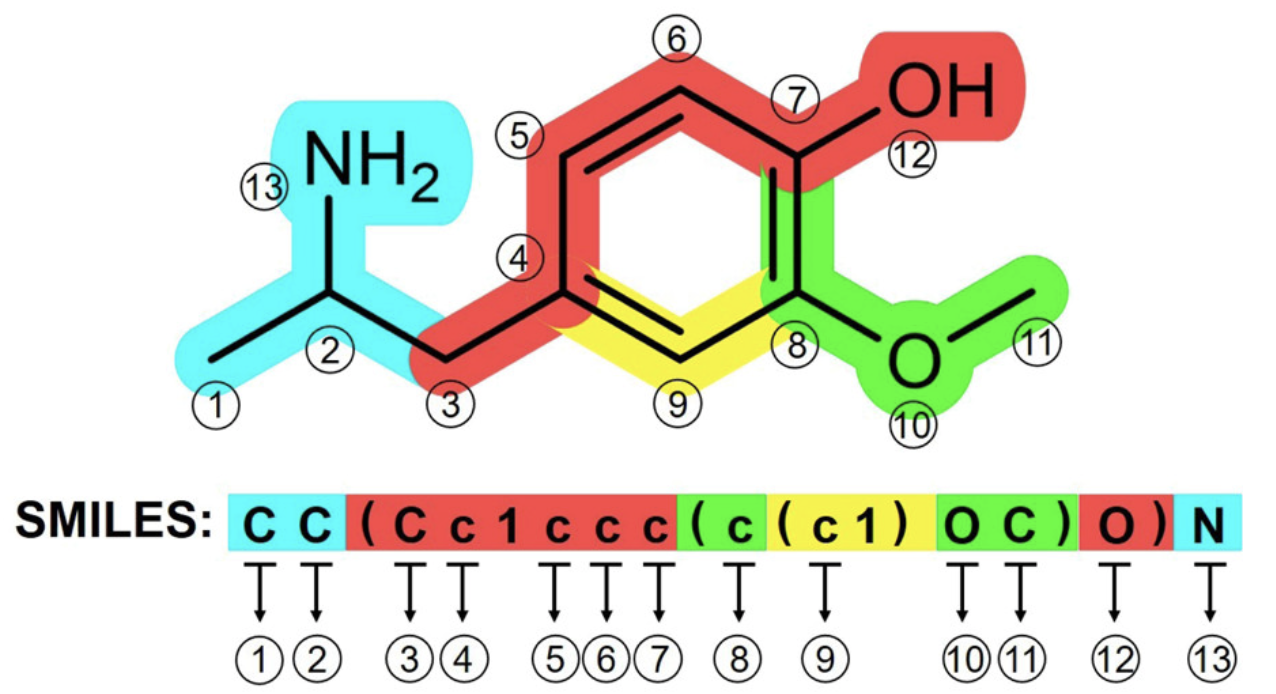
\includegraphics[width=0.8\textwidth]{Chapters/Background/Figs/smiles.png}
    \caption{\label{fig:smiles} \textbf{Illustration of the mapping from chemical structure to SMILES.} Adapted from \cite{Kim2021GenerativeCT}.}
\end{figure}

While SMILES is by far the most widely used text-based representation of molecules, other representations have been developed and are in use to address some shortcomings in SMILES. For example, the International Chemical Identifier (InChI) \cite{Heller2013InChI} string representation, which has a hierarchical construction for specifying tautomeric/stereochemical/charge states, allows greater precision and flexibility in querying molecules from large chemical databases. Another example is SELF-referencIng Embedded Strings (SELFIES) \cite{Krenn2020Selfies} which is constructed such that every SELFIES string, including random combinations of characters, is a valid molecule. This property is useful for the application of ML models that generate text as output - using SELFIES as the molecular representation, the model always output valid molecules whereas with SMILES that is not guaranteed.

\subsection{Molecular Substructures} \label{subsec:smarts}
Given a dataset of molecules or chemical reactions encoded with SMILES, we often want to identify molecules or reactions that contain a specific substructure. For example, we may want to identify molecules that contain a specific functional group or reaction that contains a specific reaction center. The standard tool for performing these substructure queries is via SMILES Arbitrary Target Specification (SMARTS) notation \cite{SMARTS}. The SMARTS line notation is expressive and allows extremely precise and transparent substructural specification and atom typing.

Using many of the same symbols as SMILES, it also allows specification of wildcard atoms and bonds, which allows expressive and precise definitons of substructures and atomic environments for searching chemical databases. One common misconception is that SMARTS-based substructural searching involves matching of SMILES and SMARTS strings. When performing a SMARTS query on a SMILES string, both SMILES and SMARTS strings are first converted to internal graph representations which are then searched for subgraph isomorphism.

\begin{table}[!h]
\begin{center}
    \begin{tabular}{|c|c|}
    \hline
        SMARTS & Substructure \\
        \hline
        [C;R] & An aliphatic carbon in a ring \\\relax
        [\#6]@[\#6] & Two carbons connected by a ring bond \\\relax
        [N;\$(NC=[O,S])] & amide or thioamide nitrogen \\\relax
        [N:1][C:2](=[O:3])[N:4]>>[N:1][C:2](=[O:3])[C:4] & urea group transforming into an amide \\
        \hline
    \end{tabular}
    \caption{Examples of SMARTS patterns}
    \label{table:smarts}
\end{center}
\end{table}

The precise substructure specification of SMARTS is useful in many aspects in the drug design process. For example, a common step in assessing the quality of a proposed drug candidate is to perform a SMARTS query to identify if the hit contains any substructures that are likely to produce artifacts in biochemical or cellular assays. These substructures are typically functional groups with a marked propensity to bind to multiple targets, so-called nuisance compounds, which are of little value in drug discovery. Many different sets of these filters have been compiled in the literature such as REOS (rapid elimination of swill) \cite{Walters1998overview} and PAINS (Pan Assay Interference Compounds) Filters \cite{Baell2010Pains}. Similarly, SMARTS queries are used to design `structural alerts' which flag molecules containing reaction chemical substructures which may lead to undesirable toxicity in the compound itself or its metabolites \cite{Limban2018StrucuralAlerts}.

Another use of SMARTS is in the labelling of pharmacophores in a molecule. Pharmacophores are an abstract description of the molecular features involved in ligand binding - typical examples of such features are hydrogen bond acceptors/donors and aromatic rings. SMARTS strings are used to map different molecular substructures to particular pharmacophore features and then to query for the presence of these features in a molecule. As with substructure filtering, different companies in the pharmaceutical industry have different/propritary sets of SMARTS strings tailored for their particular use cases. (see section \ref{subsec:pharmacophores} for details)

Beyond substructures for individual molecules, SMARTS can also be applied to reaction SMILES to capture transformation in substructures. These SMARTS strings for chemical reactions are often referred to in the literature as `reaction templates' (Fig~\ref{fig:rx_template}). Beyond querrying for matching reactions from a dataset, reaction templates can also be directly applied to a set of molecules to computationally generate a `reaction product'. This approach is used to generate virtual libraries \cite{Walters2019libraries, SaldivarGonzalez2020enumeration} \textit{in silico} both for more specific usecases such as probing the SAR of a compound as well as the construction of ultra-large commercially available compound libraries eg ZINC \cite{Irwin2020Zinc}, EnamineREAL.

% Often it is not necessary to fully simulate and understand a chemical reaction and it is sufficient to know the outcome i.e. the major product of it. This is most often the case when experimental organic chemists are willing to validate their synthetic route or when a synthesis planning software uses a reaction prediction model to score its suggestions. This is what is more traditionally referred to as reaction prediction. In these use cases a general purpose model that is able to predict a wide variety of organic reactions with good accuracy is desired. Trained organic chemists usually rationalize reactions based on the reaction mechanisms \cite{Clayden2012}. These mechanisms can be used to categorize organic reactions and each of these categories can be summarised with the help of so called reaction templates. Figure~\ref{fig:rx_template} shows a typical general reaction template for the synthesis of an amide using acid chloride and an amine. Here the $R_1$ and $R_2$ represent any chemical structures.

\begin{figure}[htbp!] 
    \centering    
    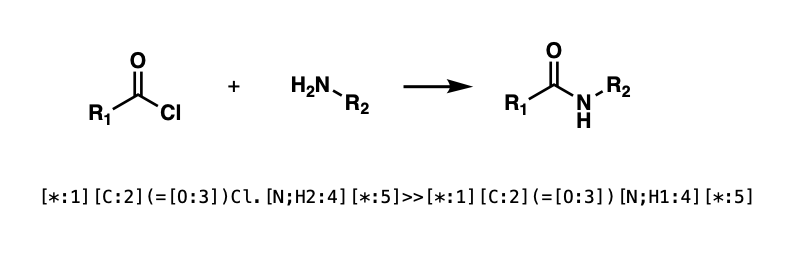
\includegraphics[width=0.75\textwidth]{Chapters/Background/Figs/rx_template_new.png}
    \caption[Reaction template]{An example of a reaction template for the synthesis of an amide from an acid chloride and a primary amine.}
    \label{fig:rx_template}
\end{figure}

In addition to virtual library construction, reaction templates can be used for organic reaction prediction by framing the problem as trying to predict the correct reaction template for a given set of reactants. Starting from a catalogue of possible reaction templates, the best matching general template in the catalogue can be found utilising subgraph searching or machine learning, and applied on the input to obtain the predicted outcome of the reaction. This approach was originally proposed for the reverse problem of retrosynthesis \cite{Corey1985ComputerAssistedSynthesis} and has had success in forward reaction prediction for the design of synthetic pathways to drug-like molecules ~\cite{Klucznik2018EfficientLaboratory}. One major limitation of template-based approaches is scalability, as the template library needs to be maintained and updated every time a new reaction is reported. A further problem is that it is often not obvious which parts of the molecule are crucial for a given reaction. This means that given a reaction one can derive a smaller more general template or a larger one that is more specific for the particular reaction. This results in either too many templates matching a particular input resulting in many equally possible reaction outcomes or in the case of larger more specific templates the library will grow very big which results in very slow predictions.

\subsection{Pharmacophores} \label{subsec:pharmacophores}

\begin{figure}[b!] 
    \centering    
    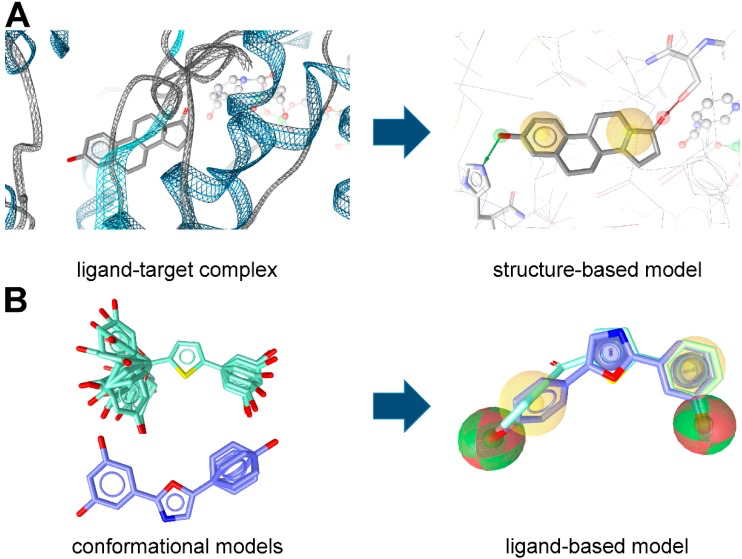
\includegraphics[width=0.75\textwidth]{Chapters/Background/Figs/pharmacophore_models.png}
    \caption{An illustration of structure-based or ligand-based pharmacophore models. Reproduced from \cite{Kaserer2015PharmacophoreReview}.}
    \label{fig:pharmacophore_models}
\end{figure}

A pharmacophore is an abstract description of molecular features that are necessary for molecular recognition of a ligand by a biological macromolecule \cite{Kaserer2015PharmacophoreReview}. A collection of pharmacophores in a geometric configuration is known as a `pharmacophore model' and it is a representation of the interactions between ligands and the binding site. By their coarse-grained nature, pharmacophore model can explain structurally diverse ligands can bind to a common receptor site, and can be used to identify novel ligands that will bind to the same receptor.

Typical pharmacophore features, characterised by SMARTS strings, include hydrophobic groups, aromatic rings, hydrogen bond acceptors or donors, and charged functional groups.

Pharmacophore models can either be constructed using structural data or from a set of active compounds \cite{Vuorinen2015pharmacophore}. In the structure-based approach, the pharmacophores are directly inferred from the observed interactions of a molecule and the binding site in experimentally determined ligand-protein complexes. (Fig \ref{fig:pharmacophore_models}A).

In the ligand-based approach, the three-dimensional (3D) structures of known active molecules are aligned and pharmacophores that are found to overlap in space are extracted as the pharmacophore model (Figure \ref{fig:pharmacophore_models}B). Although this approach circumvents the need for structural data which might not be possible to obtain, a downside is that all of the extracted pharmacophore have to be presumed as essential for protein-ligand binding, whereas in the structure-based approach it is possible to identify and discard non-important pharmacophores.

After obtaining a pharmacophore model, it can be used to virtually screen ligands from a database by identifying molecules that share similar pharmacophore features. This approach is known as `pharmacophore-based virtual screening' and is a useful tool on its own as well as for complementing molecular docking and machine learning approaches \cite{Dixon2006pharmacophore, Temml2014pharmacophore, Pradeepkiran2019pharmacophore, Pal2019pharmacophore}.

% Molecular descriptors and fingerprints based on pharmacophores have also been developed and have found to be useful as inputs for machine learning models.

\subsection{Fingerprints} \label{subsec:fingerprints}

In order to apply powerful machine learning methods, we require a (typically fixed-length) vector representation of molecules konwn in the literature as `molecular fingerprints'. The most popular molecular fingerprint is the Morgan fingerprint \cite{morgan1965fingerprints}, also known as the Extended-Connectivity FingerPrint (ECFP) \cite{rogers2010extended}. ECFPs are a particular example of `topological' fingerprints that encode the presence of substructures in a molecule by traversing the molecular graph.

ECFPs are generated via a recursive hashing algorithm that numerically hashes the representation of each atom with those of its neighbours, and again with it's next-nearest neighbours etc until a pre-defined `radius' is reached. The resulting hash values are then used to generate a fixed-length binary vector of 1/0 bits. The length of the vector is pre-determined and each 1-bit represents a unique substructure that is encountered during the traversal. The radius of the graph traversal is also a pre-defined parameter that controls the size of the substructures that are represented in the fingerprint. The radius is typically set to 2 or 3, and the length of the fingerprint is typically in the range of 1024-4096.

The popularity of the Morgan fingerprint owes to its usefullness in calculating molecular similarity \cite{Maggiora2014similarity}. Intuitively, we would expect two molecules that have `similar' molecular fingerprints to have similar chemical structures. Numerically, we can quantify the similarity between two molecular fingerprints by the Tanimoto coefficient \cite{Willet1998similarity}:

\begin{equation} \label{eqn:tanimoto}
    \mathrm{Tanimoto}(A, B) = \frac{A \cap B}{A \cup B} = \frac{A \cdot B}{|A|^{2} + |B|^{2} - A \cdot B}
\end{equation}

where $A$ and $B$ refer to the bit-vector molecular fingerprints of two molecules. The numerator $A \cdot B$ represents the number of bits shared between the two fingerprints, while the denominator represents the total number of unique bits covered by the finerprints. Two structures are usually considered similar if the tanimoto similarity is > 0.4 \cite{baldi2010similarity}. Alternate similarity measures exist but a number of comparison studies \cite{Todeschini2012tanimoto, Bajusz2015Tanimoto} have shown the Tanimoto similarity to be generally robust and consistently perform well in a variety of applications.

The combination of the Morgan fingerprint with Tanimoto similarity is useful for clustering \cite{Butina1999Clustering} datasets of similar compounds as well as performing similarity-based virtual screening. Similarity-based virtual screening relies on the  similarity property principle (SPP) \cite{johnson1990concepts}, which states that similar compounds should have similar biological activity. As a guiding strategy this means one could search a database for similar compounds to a known active molecule, and expect those compounds to retain and perhaps have improved biological activity against a target. Although this hypothesis is not always valid in cases known as `activity cliffs' where small changes in structure cause large changes in biological activity \cite{maggiora2006cliffs}, empirically it has been shown that structurally similar compounds are much more likely to be actives compared to dissimilar ones \cite{martin2002similar}. Performing similarity-based virtual screening in practice involves calculating molecular similarities between known active compounds and unkonwn molecules from a database, then selecting those with the highest similarities; ECFP4 is a consistently well-performing fingerprint for this task \cite{riniker2013benchmark, oboyle2016benchmark}.

In addition, Morgan fingerprints have also been shown to be versatile as a molecular descriptor for machine learning (ML). Machine learning models learn statistical patterns from data and can be used to make predictions on new data (see section \ref{ch:machine_learning}). In the context of drug discovery, ML can be used associate patterns in the molecular fingerprints of the molecules in a dataset with experimentally measured properties. For example, fingerprint-based models have demonstrated success in predicting physical/chemical properties such as solubility \cite{wu2017molnet}, biological activities \cite{Bender2019} as well as yields and stereoselectivities for chemical reactions \cite{sandfort2020yield}. Non-fingerprint based deep learning methods have recently been developed that learn molecular representations directly from molecular graphs, however ECFP-based shallow learning techniques continue to provide a strong, robust baseline to compare against.

\section{Computational Approaches}

\subsection{Docking}

Molecular docking is the process of predicting the binding mode of a small molecule to a protein target, and one of the most frequently used methods in structure-based drug design. \cite{meng2011molecular, Kitchen2004Docking} The binding mode is the relative orientation of the small molecule in a particular binding site of the protein, which is determined by the shapes of the binding site and molecule, and the physical interactions between the two. The binding mode has a large effect on the strength of the interaction between the small molecule and the protein, known as the binding affinity. The binding affinity, in turn, is a key determinant of the biological activity of the small molecule. The philosophy of structure-based drug design is to experimentally obtain binding modes of molecules and use this information to guide the design of new molecules by docking and choosing molecules that may have more optimal protein-ligand interactions and hence binding affinity.

\begin{figure}[!h]
    \centering
    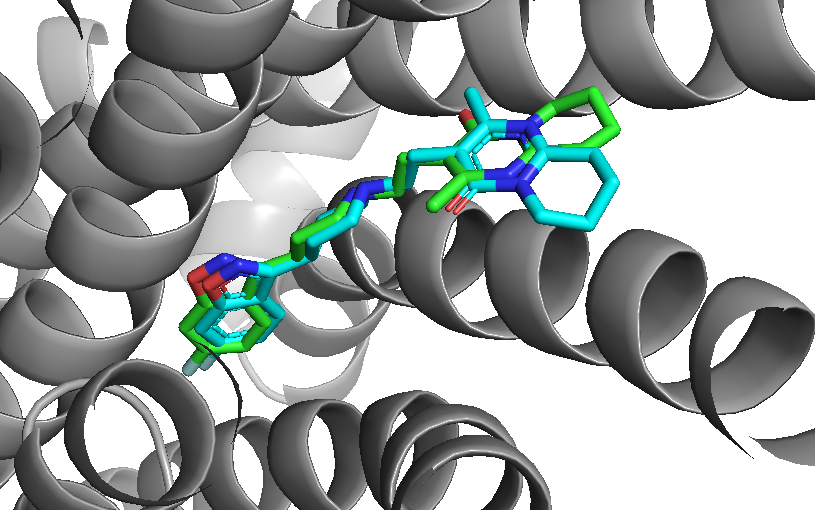
\includegraphics[width=0.8\textwidth]{Chapters/Background/Figs/docked_6a93.png}
    \caption{\label{fig:docked} \textbf{Example of a docked molecule.} The experimental structure of the ligand risperidone bound to the serotonin 2A receptor is shown in green, with the protein in grey (PDB: 6A93). The structure of the same ligand docked using GOLD is shown in cyan.}
\end{figure}

The physics of ligand-protein binding are complex, and in reality each ligand will have an ensemble of binding modes. Attempting to accurately simulate the binding process is computationally intractable, and so the goal of molecular docking is to predict the most likely binding mode. In practice this is approached as an opimisation problem, where the coordinates of the ligand and/or protein atoms are adjusted until the `best-fit' is acheived. An essential preliminary step to performing molecular docking is obtaining a structure of the protein of interest. Traditionally this means using biophysical techniques such as X-ray crystallography, NMR spectroscopy or cryo-electron microscopy (cryo-EM), but recent development in computational protein structure prediction \cite{Jumper2021AlphaFold, Wong2022AF2Docking} open the door to performing fully \textit{in-silico} structure-based drug design.

Every docking approach is essentially composed of two parts - conformation scoring and conformation searching. Potential ligand poses are ranked using a scoring function, which are typically physics-based molecular mechanics force fields that estimate the energy of the pose within the binding site. The scoring function can be composed of many components, such as electrostatic interactions, solvent and steric effects, hydrogen bonding, as well as knowledge-based potentials derived from observed interactions from databases of protein-ligand structures \cite{Li2019scoring}. While the accuracy of scoring functions has to be good enough to distinguish good poses from bad ones, major emphasis is put on computational efficiency due to the large number of evaluations required during docking. Thus, scoring functions often involve many assumptions and simplifications to reduce computational costs.

The search space of conformations is imposible to exhaustively explore as in theory it consists of all possible orientations and configurations of the protein paired with the ligand. In practice, usually the whole conformational space of the ligand is searched, while the protein is often treated rigidly. Exploration of the conformational search space is often done using stochastic methods such as Monte Carlo or genetic algorithms which randomly sample the space of conformation parameters (e.g. torsion angles) towards a minimisation of the scoring function.

The wide range of design choices for the scoring function and conformation search results in a large number of different docking algorithms that are in use in the field, such as DOCK \cite{Coleman2013DOCK}, Glide \cite{friesner2004glide}, AutoDock Vina \cite{Eberhardt2021Vina}, GOLD \cite{Verdonk2003Gold}, and FRED \cite{McGann2012FRED}. The relative performance between these docking algorithms are typically retrospectively evaluated by directly comparing predicted binding poses to known crystal structures of ligand-protein complexes. The benchmark datasets used for this purpose are typically high-quality structures of drug-like molecules such as PDBbind \cite{Wang2004PDBbind,Liu2014PDBbind}. There are also community assessments on the relative prospective performance of different docking approaches \cite{Parks2020D3R} and scoring functions \cite{Su2019CASF}.

Besides the structural focus of binding pose prediction, increasingly in recent years docking has been used to directly virtually screen large databases of molecules in silico to identify molecules that are likely to bind to protein target of interest \cite{Bender2021LargeScaleDocking}. This approach puts the focus on the scoring function, with the rationale that molecules with high docking scores are much more likely to be active than those with low scores. In this scenario, success is defined by the enrichment of active compounds in the top ranks of a docking screen, measured via the enrichment factor:

\begin{equation}
    \mathrm{EF}(n) = \frac{\mathrm{Hit\: rate (predicted\: top - }n)}{\mathrm{Hit\: rate (baseline)}}
\end{equation}

where the baseline hit rate is the proportion of actives in the dataset overall, representing the performance of simple random ordering. Different methods are benchmarked by retrospectively evaluating the enrichment factor of known ligands from a large database of presumed non-binding, “decoy” molecules for multiple protein targets - the classic benchmark dataset for this is the Directory of Useful Decoys (DUD) \cite{Huang2006DUD, Mysinger2012DUDE}.

Prospectively, large-scale virtual screening with molecular docking has had notable successes. A review specifically looking at G protein-coupled receptors (GPCRs) \cite{Ballante2021DockingGPCR}, which are the target of more than 30\% of all marketed drugs, showed 62 successful virtual screens for 22 unique protein targets belonging to 14 different receptor families in the past decade. Of particular note is that increasing availability of computational resources, together with increases in the sizes of commercially-available make-on-demand compound libraries, has made possible ultra-large virtual screening campaigns against libraries of >100 million compounds  \cite{Lyu2019UltraLargeDocking, Alon2021sigma, Fink2022Alpha}. At the same time, limitations in the accuracy of scoring functions and in the modelling of protein flexibility \cite{Erickson2004flexibility, Antunes2015flexibility} restrict the ability of docking to reliably distinguish active molecules from inactive ones \cite{Llanos2021StrengthsAndWeaknesses, Macip2022HasteMakesWaste}, leading to false positives which are exacerbated when screening large libraries \cite{Lyu2023Expansion}.

In the absence of exisiting ligand bioactivity measurements for a protein target, virtual screening with molecular docking remains the only computational method of choice and is a default starting point for beginning drug discovery against a brand new target. However, there has been recent results claiming that deep learning models which use neural networks to directly generate ligand binding poses \cite{Stark2022equibind, corso2023diffdock} outperform docking algorithms in terms of accuracy. These results are promising and, coupled with continued advancements in protein structure prediction to account for protein flexibility, suggest that deep learning may be a viable alternative to molecular docking for binding pose prediction and virtual screening in the coming years.

\subsection{Machine Learning} \label{ch:machine_learning}

Machine learning (ML) refers to the use of algorithms that `learns' how to make predictions or decisions based on observed data. By designing models that can learn patterns directly from input data, it is found that ML methods can often surpass manually created algorithms by humans on a wide variety of tasks. In the following paragraphs, we provide an overview of the ML concepts and ideas needed to understand the research presented in this thesis. We will focus on supervised learning and neglect many important sub-fields such as reinforcement learning and generative models which are more described in greater detail in refs \cite{Bishop2006PatternRecognition,Goodfellow2016DeepLearning}.

Very broadly, the aim of machine learning is to learn the parameters $\theta$ of a predicative model $y = f (x, \theta)$ that minimise a given cost function, $\mathcal{L}(y, \hat{y})$, where $x$ is a given input, $y$ is the target variable and $\hat{y}$ is the predicted value, i.e. to find the solution

\begin{equation}
    \hat{\theta} = \arg\min_{\theta} \mathcal{L}(\theta)
\end{equation}

For regression, which is the modelling of a continuous variable, the most common loss function choice is the squared residuals,

\begin{equation}
    \mathcal{L}(y, \hat{y}) = \sum_{i}(y_i - \hat{y}_i)^{2}
\end{equation}

while for binary classification, which is the task of predicting which class an input $x$ belongs to, the most common loss function is the binary cross-entropy loss:

\begin{equation}
    \mathcal{L}(y, \hat{y}) = -\sum_{i}y_i\log(\hat{y}_i) + (1 - y_i)\log(1 - \hat{y}_i)
\end{equation}

where the target variable $y$ can be either 0 or 1 while the predicted value $\hat{y}_i$ is the predicted probability of class 1 and $1-\hat{y}_i$ is the predicted probability of class 0.

To find the solution $\hat{\theta}$ for a dataset in practice, we would first divide the input data into training, validation and test sets. The model is initially fit on the training data set, where the data-dependent parameters of the model (e.g. the coefficients of a polynomial regression model) are optimised to minimise the loss function. Afterwards, the fitted model is used to make predictions on the validation data set. The validation data set provides an unbiased estimate of the model's performance on the training data set for the purpose of tuning the non-data-dependent parameters, known as `hyperparameters', of a model (e.g. the number of degrees to include in a polynomial regression model). This process may be repeated multiple times, with the model's performance on the validation data set being used to select the best hyperparameters. This overall process is known as `training a model'.

After a model has been trained we use the test dataset, which has never been seen by the model during training, to evaluate the performance of the model. It is important to use the same training and test datasets for a fair comparison of different models, and curated datasets from the literature are commonly used as a benchmark for evaluating the performance of new models.

For regression models, the most common metric used to evaluate the performance of a model is the root mean squared error (RMSE) or the pearson correlation coefficient (PCC). For binary classification models, the most common metric used is the area under the receiver operating characteristic curve (AUC). The receiver operating characteristic (ROC) curve is created by plotting the true positive rate (TPR) against the false positive rate (FPR) as the discrimination threshold for classifying one class over the other is varied \ref{fig:roc_curve}. The AUC is the area under the ROC curve, and is a measure of the model's ability to distinguish between the two classes. AUC values range from 0 to 1, with 0.5 indicating a model that is no better than random guessing, and 1 indicating a perfect model.

\begin{figure}[htbp!] 
    \centering    
    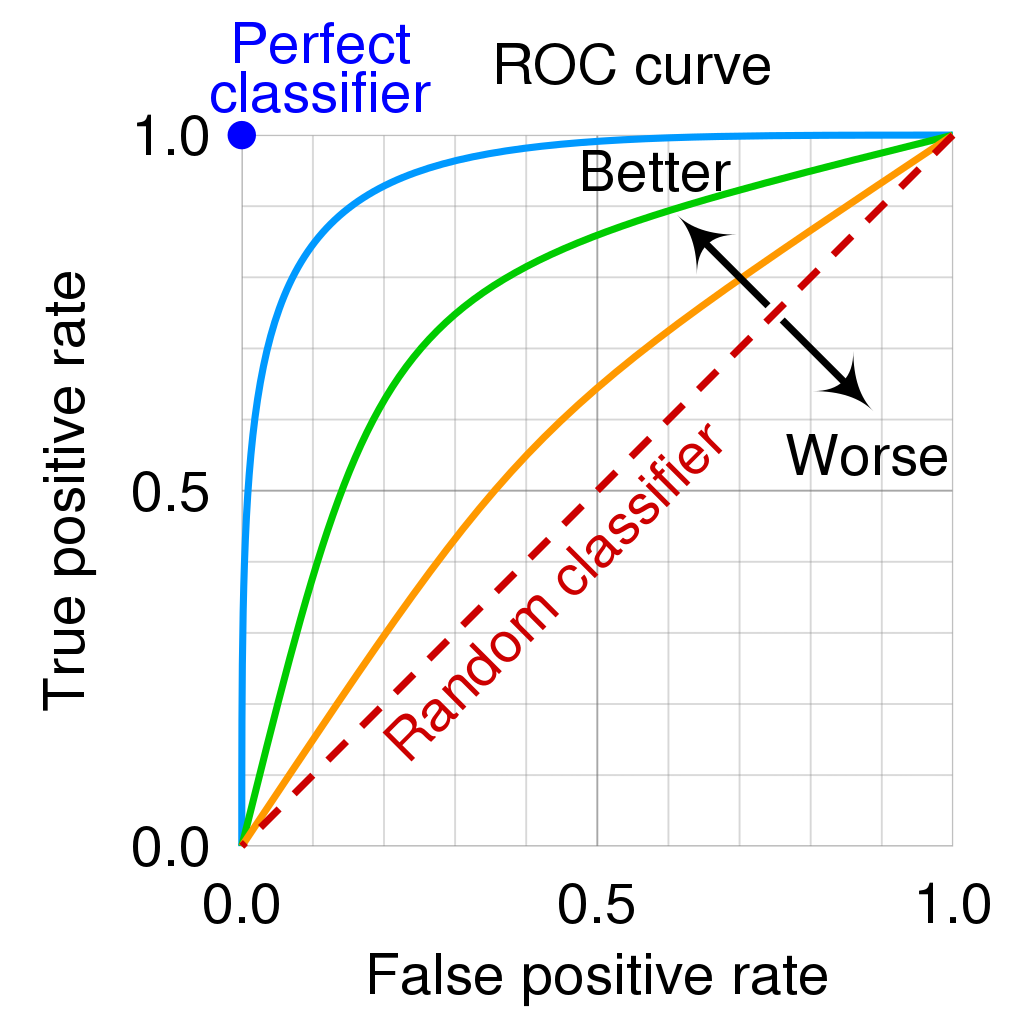
\includegraphics[width=0.75\textwidth]{Chapters/Background/Figs/roc_curve.png}
    \caption{An example Receiver Operating Characteristic (ROC) curve. The diagonal shows the performance of a random classifier. Three example classifiers (blue, orange, green) are shown. Reproduced from \cite{roccurve}.}
    \label{fig:roc_curve}
\end{figure}

A large number of machine learning techniques have been described and applied for drug discovery, and an overview of them can be found in \cite{Bender2021part1,Bender2021part2,Volkamer2023review}. In this thesis, two common techniques are used: Random forests and Gaussian processes.

\subsubsection{Random Forest}

Random Forest models are ensemble learning methods that utilise a large number of decision trees for making predictions \cite{Breiman2001RF}. For classification tasks, the output of the random forest is the class selected by most trees. For regression tasks, the output is the mean of the predictions by the individual trees:

\begin{equation}
    f(x) = \frac{1}{N}\sum^{N}_{i} f_{i}(x)
\end{equation}

where $f_{i}$ is the $i$th tree in the forest and $N$ is the total number of trees in the forest. Decision trees are constructed to succerssively split the data into branches via `decision boundaries' (e.g. $x > 1.5$). Decision boundaries are chosen to minimise the square deviations (for regression) or information entropy (for classification) between the samples and the sample mean in each branch or leaf of the tree. 

Although extremely computationally efficient and interpretable, individual decision trees are very prone to over-fitting. By using a large number of decision trees each trained on different random subsets of the data (a process known as bootstrap aggregation), random forest models can acheive a lower variance and hence improved performance. To further reduce correlation between the decision trees, random forests use random feature selection, where only a random subset of the features are considered for each decision boundary.  

Random forests are relatively easy to use, require little tuning of hyperparameters, and are robust to over-fitting, and thus are a popular general machine learning technique. In particular for drug discovery, random forests have been extensively used with molecular fingerprints features for prediction of properties such as solubility \cite{Palmer2007RandomForest}, biological activity \cite{Svetnik2003RandomForest, Merget2017KinaseInhibitors}, and toxicity \cite{Polishchuk2009RandomForest}.

\subsubsection{Gaussian Process}

Gaussian Process models are a kernel-based method that utilises what is known as the `kernel trick' to calculate high-dimensional weighted averages \cite{rasmussen2005gp}. The kernel trick is the use of a kernel function to calculate the inner product between the features vectors of two datapoints in a high-dimensional feature space without explicitly computing higher-dimensional feature vectors. A typical kernel function is the squared exponential kernel:

\begin{equation}
    \mathcal{K}(x , x') = \exp\left(-\frac{\|x - x'\|^{2}}{2l^{2}}\right)
\end{equation}

where $l$ is the length scale of the kernel, a hyperparameter that determines how quickly the function can change, and $x$ and $x'$ are the feature vectors of the datapoints in the initial low-dimensional feature space. Mathematically, the kernel trick enables the construction of models that are, in theory, infinitely complicated with a finite amount of computation \cite{Hofmann2008kernel}. Gaussian Processes utilise the kernel function to calculate the covariance matrix of the Gaussian distribution over the function values. The covariance matrix is then used to calculate the posterior distribution over the function values given the training data, which can then be used to make predictions on new data with associated uncertainty values.

The fact that GPs have few hyperparameters to tune and maintain uncertainty estimates over property values have also led to their use for molecular property prediction \cite{Obrezanova2007GPQSAR, McCorkindale2020Soap, Jorner2021ActiviationEnergiesGPR}, in particular incorporating the Tanimoto similarity in the kernel function \cite{Swamidass2005kernels, Griffiths2022photoswitches}.

\subsubsection{Deep Learning}

In contrast to methods which use hand-crafted features as input (`shallow learning'), deep learning revolves around learning representations directly from the raw data using neural networks. Neural networks are composed of layers of `neurons' that successively perform non-linear transformations on their inputs, mimicking the way that biological neurons transfer signals to one another. These transformations are typically of the form:

\begin{equation}
    \textbf{h} = \sigma(\mathbf{W} \cdot \mathbf{x} + \mathbf{b})
\end{equation}

where $\mathbf{W}$ is a weight matrix, $\mathbf{x}$ is a vector of inputs, $\mathbf{b}$ is a vector of biases and $\sigma$ is an optional non-linear activation function. The output of the layer is the vector $\mathbf{h}$, which is either input to the next layer or taken as the output of the model. The weights $\mathbf{W}$ and biases $\mathbf{b}$ from all of the layers collectively are the parameters $\theta$ of the neural network that are learned by fitting on data.

Deep learning has found remarkable success in a wide range of applications, including computer vision \cite{Wang2020CLIP}, natural language processing \cite{OpenAI2021GPT3}, speech recognition \cite{Schneider2019wav2vec}, and bioinformatics \cite{Jumper2021AlphaFold, Sapoval2022Bioinformatics}. This is because of the ability of neural networks to learn complex, non-linear relationships between inputs and outputs in the presence of large amounts of data. `Big data' domains are computationally intractable for shallow learning methods, but deep learning can be successfully applied as neural networks can be optimised effectively using  gradient-based approaches, such as gradient descent:

\begin{equation}
    \theta_{t+1} = \theta_t - \eta \nabla_{\theta} \mathcal{L}
\end{equation}

where at each step $t$ the model's parameters are updated according to the learning rate $\eta$, a hyperparameter of the optimiser. Instead of calculating the gradient of the loss $\nabla_{\theta}\mathcal{L}$ on the full training set, standard practice is to use a stochastic approximation of the gradient that is calculated from a randomly sampled batch of training data. This significantly speeds up the optimisation process and allows neural networks to be trained on large datasets that would otherwise be intractable. These stochastic gradient steps are iterated repeatedly over the training set until the value of the loss has satisfactorily converged. 

The gradient of the loss function with respect to the model parameters can be obtained efficiently by applying the chain rule via a process called `backpropogation'. Using automatic differentiation frameworks that can be carried out on hardware accelerators, such as graphical processing units (GPUs), the time needed to train neural networks are dramatically reduced \cite{Baydin2018autodiff}. Further improvements to model optimisation can be achieved by incorporating more sophisticated optimisation algorithms, such as Adam \cite{Kingma2014Adam}, as well as the use of regularisation techniques such as dropout \cite{Srivastava2014dropout} and batch normalisation \cite{Ioffe2015batchnorm}, and remains a significant area of active research.

The only constraint on the design of a neural network is that the mathematical operations in the model must have defined derivatives so that the gradient of the loss function can be calculated with backpropagation for efficient training. This results in a zoo of different neural network designs (referred to as `architectures') that use differentiable building blocks with specific inductive biases tailored to the task at hand. For example, convolutional neural networks (CNNs) utilise built-in translational invariance for computer vision applications (e.g. AlexNet \cite{Krizhevsky2012AlexNet}, and ResNets \cite{He2015ResNet}) while recurrent neural networks (RNNs) designed for learning temporal dependencies are applied to sequential data such as text \cite{Cho2014RNN} and speech \cite{Lipton2015RNN} (e.g. Gated-Recurrent-Unit (GRU) \cite{Chung2014GRU} and Long-Short-Term-Memory (LSTM) networks \cite{Hochreiter1997LSTM}). 

In the context of drug discovery, the challenge of modelling molecular inputs has led to the devlopment of graph-based neural network architectures known as `graph neural networks' (GNNs). These models are designed to learn representations of molecular graphs that are invariant to the order of the nodes and edges. GNNs have been successfully applied to a range of molecular tasks, including molecular property prediction \cite{wu2017molnet,Gilmer17mpnn, Mayr2018compare, yang2019chemprop}, and predicting reaction templates for input reactants \cite{Coley19WLDN5}. More standard architectures such as Transformer models developed for natural language processing have also been applied to SMILES, as well as three-dimensional voxel-based CNNs which can be trained on protein-ligand complexes for the prediction of binding affinity \cite{Ragoza2017ProteinCNN,Imrie2018ProteinCNN,Jimenez2018Kdeep}.

Neural networks can also be used with pre-computed features such as molecular fingerprints. Example applications include the use of bioactivity prediction \cite{Bender2019}, reaction prediction \cite{Wei2016reactionprediction, segler2017neural}, and the prediction of docking scores \cite{Gentile2020deepdocking}.

Despite their success in certain molecular tasks, deep learning still has several limitations when it comes to drug discovery. Chief among these is the need for large amounts of training data for strong performance, which can often be costly and time-consuming to obtain. When only a small amount of data is available, which is typical in the early stages of drug discovery, neural networks may perform worse than simpler shallow learning models \cite{Jiang2021benchmark}. 

Additionally, neural networks may struggle to generalize to new molecules that are substantially different from the molecules in the training set. This is known as the `generalization gap' and model performance with typical random-split cross-validation procedures do not accurately reflect the true generalization performance of the model \cite{Sheridan2013TimeSplit}. This has led to a growing movement towards measuring model performance using `scaffold split' \cite{wu2017molnet, yang2019chemprop} or `time split' \cite{Sheridan2013TimeSplit} cross-validation, which splits the data into disjoint sets of molecules that are similar in structure or time of data acquisition, respectively. This allows for a more accurate assessment of the generalization gap, but this remains a challenge for applying deep learning and machine learning models in general in drug discovery.

Another challenge is the lack of interpretability of neural network models, which make it difficult to understand the underlying reasons for a model's predictions. Without explainations of model predictions, it becomes difficult to avoid correct predictions for the wrong reasons (the so-called clever Hans effect) \cite{Lapuschkin2019UnmaskingCleverHans}, avert unfair biases, and gain potentially useful insights from the model. This is a challenge in general for deep learning, but is particularly difficult in drug discovery due to the domain-specific complication of projecting `explanations' onto molecule representations \cite{Jimenze2020XAI}.

Accounting for these limitations are critical for realizing the full potential of applying both shallow and deep learning models to accelerate the design-make-test cycle in drug discovery.

% In the paper of Nam and Kim \cite{Nam2016LinkingReactions} they formulated the reaction prediction problem as a translation task. The input SMILES corresponding to the reactant and reagent molecules are tokenized, so that each character of SMILES is equivalent to a word and the whole input is equivalent to a sentence. This sentence is than ``translated" by the model to the product SMILES. Neural machine translation models are trained using a large parallel corpus. This is available in the case of organic reactions from patents and publications or can be generated using templates of elementary reactions. The method of Nam and Kim served as an important proof of concept but could not match the accuracy of rule-based and graph-to-graph models. \par
% %The method was built on a neural network building block called gated recurrent unit (GRU) \cite{Cho2014LearningTranslation}. GRUs are a type of recurrent neural networks that process arbitrarily long inputs token by token, so that the hidden state representation of each token depends on the previous ones. %The model used in the paper is illustrated on Figure~\ref{fig:gru}. 
% %This model served as a proof-of-concept but could not match the accuracy of graph-to-graph and template based approaches. \par

% \iffalse
% \begin{figure}[htbp!] 
% \centering    
% \includegraphics[width=0.9\textwidth]{Chapter2/Figs/Raster/gru.png}
% \caption[GRU for reaction predictions]{The architecture used by Nam and Kim. The input SMILES string is tokenized into ``words", each token is embedded using a learnt embedding and processed by a three layer GRU network. The product is generated using attention mechanism.}
% \label{fig:gru}
% \end{figure}
% \fi

% The large breakthrough of sequence-to-sequence models for reaction prediction came after the introduction of a new and innovative architecture for neural machine translation by Vaswani et. al. \cite{Vaswani2017}. The so called Transformer model revolutionized the entire industry of machine translation and found use in many other areas of machine learning ever since. In the next section the Transformer architecture is described in detail followed by a discussion of the Molecular Transformer. 

% \section{The Molecular Transformer}

% \subsection{The Transformer architecture}

% The Transformer architecture was originally developed for machine translation tasks. It has an encoder-decoder structure. Both the encoder and the decoder are made up of so called transformer blocks that process the inputs by applying a multi-head scaled dot-product attention mechanism followed by layer normalization and some fully connected feed forward layers. In the following each part is described in detail. 

% \subsubsection{Encoder}
% The input to the model is a sentence made up of different words that are contained in a vocabulary. Each word in the vocabulary has a learnt fixed-length vector representation. Passing these vectors to the model would not be enough though as these vectors have no reference to where the given word appears inside the sequence. To encode this information as well another vector of the same length is added to each word-vector that depends on the position inside the sequence: \par

% \begin{equation}
%     PE_{(pos, 2i)}=\sin(pos/10000^{2i/d_{model}})
% \end{equation}
% \begin{equation}
%     PE_{(pos, 2i+1)}=\cos(pos/10000^{2i/d_{model}})
% \end{equation}

% This vector representation of the input text is passed into the transformer blocks. These consist of a multi-head attention layer with residual connection \cite{He2016DeepRecognition} followed by layer normalization \cite{Ba2016LayerNormalization} and a 2-layer fully connected feed forward neural network with ReLU activation. The encoder of the model is made up of $N=6$ transformer blocks as illustrated on Figure~\ref{fig:transformer}

% \begin{figure}[ht]
% \centering    
% \includegraphics[width=2.9in]{transformer_diagram.png}
% \caption{Graphical illustration of the full transformer model \cite{Vaswani2017}}
% \label{fig:transformer}
% \end{figure}

% \subsubsection{Multi-head scaled dot-product attention}
% The multi-head scaled dot-product attention is the heart of the Transformer model. It is a specific version of a general deep learning technique called attention. Given a set of vector \emph{values} and a vector \emph{query} the attention mechanism computes a weighted sum of the \emph{values} dependent on the \emph{query}. The sum represents a selective summary of the \emph{values} and the \emph{query} determines the importance of each vector, i. e. determines how much each \emph{value} vector is attended to.\par 
% The full attention mechanism operates by performing the following steps. Given some vector values $\bm{h_1}, \bm{h_2},\dots, \bm{h_N} \in \mathbb{R} ^{d_1}$ and a query $\bm{q} \in \mathbb{R} ^{d_2}$ \par

% \begin{enumerate}
%     \item First the attention scores $\bm{e} \in \mathbb{R}^N$ are computed. In the case of the scaled dot-product attention $d_1=d_2$ and $\bm{e}$ is simply defined as the scaled vector of projections $e_i=\frac{\bm{q}^\intercal \bm{h}_i}{\sqrt{d_1}}$
%     \item To generate the attention distribution $\bm{\alpha}$ the softmax of $\bm{e}$ is taken: 
%     \begin{equation}
%         \alpha_i=\frac{\exp{(e_i)}}{\sum_{j=1}^N \exp{(e_j)}} 
%         \label{eqn:softmax}
%     \end{equation}
%     \item Finally the attention distribution is used to take the weighted sum of the values to obtain the final output
%     \begin{equation}
%         \bm{a}=\sum_{i=1}^N \alpha_i \: \bm{h}_i \; \in \mathbb{R}^{d_1}
%     \end{equation}
% \end{enumerate}

% The scaling factor in the dot product serves the purpose of preventing some of the projection becoming overwhelmingly large which in turn would lead to the softmax function being sharply peaked around those values and being shallow everywhere else. This would result in very small gradients at most places that can substantially slow down the training.\par

% In the Transformer encoder the above described attention mechanism is used such that given a set of input vectors a new vector is calculated for all of them (being the query) from the others (being the keys). This is called self-attention. This way during training the model is able to learn which vectors (that are representing words or atoms) usually interact with each other. This interaction can result in a large value in the attention distribution. \par

% Usually the input, be it a chemical formula or a sentence contains a rich structure with the words affecting each others meanings in multiple ways. The problem with the simple self-attention mechanism is that by defining a single attention distribution for each input vector only one way of interaction can be learnt by the model. To give the model more flexibility to potentially learn more complex interaction structures multi-head attention was introduced. This mechanism maps the vectors to $h=8$ different lower dimensional spaces via a set of learnt linear transformations. The self-attention mechanism is than applied in these lower dimensional spaces simultaneously. The outputs of the different attention heads are finally concatenated and fed into a linear neural network layer. The whole mechanism is illustrated on Figure~\ref{fig:multihead_attention}

% \begin{figure}
% \centering    
% \includegraphics[width=2.2in]{mulithead_attention.png}
% \caption{Graphical illustration of the multi-head attention \cite{Vaswani2017}}
% \label{fig:multihead_attention}
% \end{figure}

% \subsubsection{Decoder}

% The outputs of the encoder which are $N$ vectors if the input sequence is $N$ words long are fed into the decoder which has a structure almost identical to the encoder. The first modifications concern the masking in the multi-head self-attention layers to make sure that every token in the output translation can only attend to the preceding ones. The second modification of the attention mechanism is making use of the encoder outputs by using them as keys whilst the queries are the outputs of the previous decoder layer. \par
% The generation of the translation happens in a sequential manner. First the embedding of the special \texttt{<start>} token is fed into the decoder and passed through the layers. The result is projected to a vector that has the same dimensionality as the size of the vocabulary. Finally the softmax function is applied to obtain the probability of the first word. The second word is generated by passing in the first word (and the \texttt{start} token) to the decoder, the third is generated by passing in the first and the second etc. This is called autoregressive translation. Finally the translation terminates either when the most probable next token is the special \texttt{<end>} token or when the maximum sequence length is reached. By multiplying together the next-token probabilities and normalizing with respect to the length of the output a confidence score of the translation can be obtained. 


% \subsubsection{Datasets}
% The first dataset used in this work is the freely available USPTO dataset \cite{Lowe2012} that was filtered by Jin et. al. \cite{Jin2017}. Further filtering was preformed to remove some remaining duplicates or reactions that were erroneously text mined. These included examples such as reactions whose sole product is nitric acid, sulfuric acid, chloride ion etc. This way the final number of reactions in the dataset was 471 791 of which 377 419  were used for training, 23 589 for validation and 70 765 were used as a hold-out test set. The training set was augmented by an equal number of random equivalent SMILES strings. Augmentation can help the model to learn the underlying molecular graph from the SMILES sequence. \par
% The model trained in the way described above achieved 88.8\% Top-1 accuracy on the test set. This model was used throughout the interpretability experiments and is referred to as USPTO Transformer. \par
% The second dataset used was the commercial Pistachio dataset \cite{Mayfield2018Pistachio2.0}. This dataset contains over 9 million reactions text mined from US and EPO patents. This dataset was filtered similarly to USPTO to remove erroneous and duplicate reactions. It turned out that many of the 9 million reactions were duplicates corresponding to different patent IDs. In the end a dataset of 2 375 385 reactions was obtained of which 2 019 078 was used for training, 118 770 for validation and 237 537 for testing. \par
% The model trained as described above achieved 76.4\% Top-1 accuracy on the test set. Even though this looks like a substantially lower performance in reality the two models perform similarly well on new reactions. The possible reasons for the large difference in the measured performance on the held-out test sets are described in detail in Chapter~\ref{chap:interpr_molt}. This model obtained was also used in the interpretability experiments to test the effect of increased training set size on the models understanding of chemistry and is referred to as Pistachio Transformer in the rest of the thesis. \par

\chapter{Hit Discovery via Unsupervised Learning of Fragment-Protein Complexes} \label{ch:fresco}

% ... This chapter ...

% The process of finding molecules that bind to a target protein is a challenging first step in drug discovery. Crystallographic fragment screening is a strategy based on elucidating binding modes of small polar compounds and then building potency by expanding or merging them. Recent advances in high-throughput crystallography enable screening of large fragment libraries, reading out dense ensembles of fragments spanning the binding site. However, fragments typically have low affinity thus the road to potency is often long and fraught with false starts. Here, we take advantage of high-throughput crystallography to reframe fragment-based hit discovery as a denoising problem -- identifying significant pharmacophore distributions from a fragment ensemble amid noise due to weak binders -- and employ an unsupervised machine learning method to tackle this problem. Our method screens potential molecules by evaluating whether they recapitulate those fragment-derived pharmacophore distributions. We retrospectively validated our approach on an open science campaign against SARS-CoV-2 main protease (Mpro), showing that our method can distinguish active compounds from inactive ones using only structural data of fragment-protein complexes, without any activity data. Further, we prospectively found novel hits for Mpro and the Mac1 domain of SARS-CoV-2 non-structural protein 3. More broadly, our results demonstrate how unsupervised machine learning helps interpret high throughput crystallography data to rapidly discover of potent chemical modulators of protein function. 

% \section{Introduction}

Hit detection is a key step in the early stages of the drug discovery process following the identification of a biological target of interest \cite{Hughes2011Principles}. A `hit' compound acts as the starting point for the drug design process where the chemical structure of the hit is progressively optimised towards a candidate drug. Approaches towards hit detection generally involve screening large libraries of compounds, both experimentally and computationally.

% Approaches towards hit detection generally involve the screening of libraries of compounds. For example, in high throughput screening (HTS) often hundreds of thousands of chemical compounds are synthesised and tested, requiring substantial resources as well as complex logistics. While experimental techniques such as DNA-Encoded libraries are being developed to increase the efficiency of large-scale compound screening \cite{GirondaMartinez2021DNALibrary}, there has been a growing push towards conducting hit detection computationally instead to decrease the cost and accelerate this step of the drug discovery process \cite{?}. 

% In this approach, known as virtual screening, a computational scoring function is used to estimate the potency of a compound. After computing the scores for all of the compounds in a library, only those ranked highly by the scoring function are chosen for synthesis and experimental validation. Currently the predominant scoring function used to conduct a virtual screen is molecular docking. In molecular docking, the 3D conformation of a ligand and the target are explicitly modelled and a physics-based simulation of the binding process is conducted, with the calculated energy of the bound ligand as the score. Although this approach has yielded success \cite{Lyu2019UltraLargeDocking,Alon2021SigmaTwo}, correctly performing molecular docking is non-trivial and the deficiencies of molecular docking for bioactivity prediction are well-documented \cite{Llanos2021StrengthsAndWeaknesses, Macip2022HasteMakesWaste}.

% An alternative to these methodologies is fragment-based drug discovery (FBDD). In this approach, a library of very low molecular weight compounds (`fragments' typically less than 18 nonhydrogen atoms \cite{David2017FBLD}) are screened at high concentrations alongside the generation of bound fragment-protein structures via X-ray crystallography or cryo-EM. By obtaining these experimental structures and examining the binding interactions between individual fragments with protein residues, fragments can be used as building blocks for larger molecules by linking or merging together disparate fragments in order to increase potency. Conceptually, FBDD is based on a coarse-graining of fragments to specific moieties or groups that are associated with interactions to the target, with the goal of maintaining and optimising these interactions in larger molecules.

One of these methodologies is fragment-based drug design (FBDD). In this approach, very low molecular weight compounds (`fragments' with typically less than 18 nonhydrogen atoms \cite{David2017FBLD}) are screened at high concentrations against the target protein with X-ray crystallography. A fragment screening approach is more likely to deliver hits than screening larger drug-like molecules because low molecular complexity compounds are more likely to possess good complementarity with the target protein \cite{hann2001molecular}. Structures of these fragment-protein complexes can then inspire the design of potent binders, either by expanding a fragment to pick up new intermolecular interactions with active site residues, or merging together different spatially proximal fragments \cite{Ichihara2011FragLinking, Yu2021FragLinkingEntropy}. However, despite showing up in X-ray crystallography, the binding affinity of the fragments themselves is typically low. Therefore, gaining potency by fragment expansion or merging is typically a long journey fraught with false starts. 
%Further, data throughput is historically low due to difficulties in setting up crystallization and refinement workflows. As such only small fragment libraries can be screened, resulting in a handful of fragment hits. 

%Conceptually, FBDD is based on a coarse-graining of fragments to specific moieties or groups that are associated with interactions to the target, with the goal of maintaining and optimising these interactions in larger molecules.

% \begin{figure}
%     \centering
%     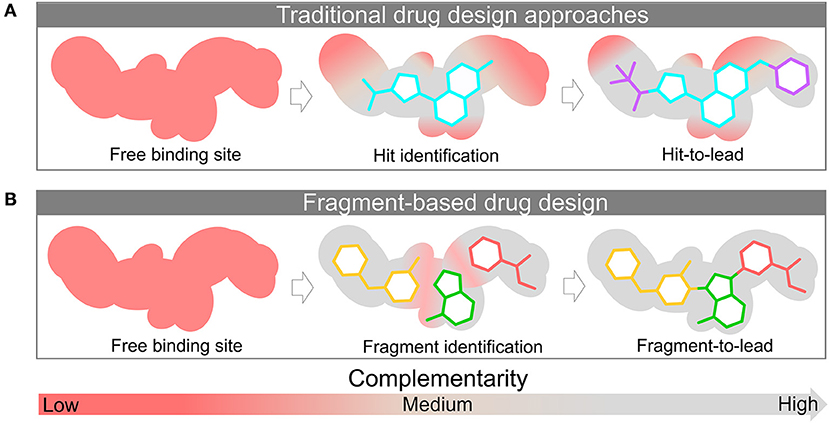
\includegraphics[width=\linewidth]{Chapters/Fresco/Figs/fbdd_vs_trad.jpg}
%     \caption{An illustration comparing fragment-based drug discovery to traditional approaches.}
%     \label{fig:fbdd}
% \end{figure}

Recently, advances in X-ray crystallography such as automatic crystal mounting robots, fast detectors, as well as increased accessibility to beamtime are enabling high throughput fragment screens. One can routinely go from screening a small fragment library and detecting a handful of hits, to screening 1000s of fragments with ensembles of 100s of fragments hits spanning the binding site \cite{Schiebel2016HighThroughput, Douangamath2020XChem}. This substantial increase in data enables a systematic data-driven approach for fragment-based hit discovery. 

% Although there exist some computational approaches for supporting FBDD, for example hot spot analysis and pocket druggability prediction \cite{deSouza2020InSilicoFBDD}, at present the main procedure of selecting which fragments to merge and how to do so remains largely intuition-based and human-driven.

%Follow up compounds are then designed using chemical intuitions to merge spatially proximal fragments, or expand a fragment into promising binding pockets \cite{Ichihara2011FragLinking, Yu2021FragLinkingEntropy}. 

%Factoring in the rise of cryo-EM techniques as well \cite{Renaud2018CryoEMReview, Callaway2020RevolutionaryCryoEM}, we are reaching the stage where the data output will outpace traditional approaches for hit detection via FBDD. Let us consider the standard method of merging or linking pairs of fragments: given $N$ fragment hits, there are $\frac{N(N-1)}{2}$ possible choices of fragment pairs that could be combined. This means that if a fragment screen returns 100 hits, there are 4950 fragment pairs that have to be considered, and for each of these pairs there are many possible ways to merge/link them into a potential hit compound.

%How to select a particular pair from these options, as well as how to actually perform the merging/linking of these fragments, remains largely intuition-based and human-driven \cite{Ichihara2011FragLinking, Yu2021FragLinkingEntropy}. Of course not all of these possible pairings are chemically reasonable, but the overall quadratic scaling points to a growing headache where fragment screens give too many options to choose from, where increased data raises more questions than answers.

%When data throughput outstrips manual expertise, machine learning (ML) may provide the solution. By taking advantage of underlying patterns in large datasets, ML methods have recently provided breakthroughs in scientific domains such as protein-folding, chemical reaction prediction, and improving functionals in density functional theory. In the context of FBDD, ideally we would like to use machine learning to leverage all of the available crystal structure data to inform our decision making when advancing from a fragment screen towards hit detection. However, how to do so conceptually in terms of data featurization or model design has to the authors' knowledge never been discussed, let alone experimentally experimentally validated for hit detection.

Our key insight is to reframe fragment-based drug design as signal extraction from noisy data by seeking persistent pharmacophore correlations within a fragment ensemble, rather than looking at individual fragments. This is because a fragment itself has low affinity, thus we need the presence of multiple fragments with the same pharmacophore at a particular region of the binding site to provide statistical confidence. 

In this chapter, we employ unsupervised machine learning to learn the spatial distribution of fragment pharmacophores in the binding site. We then use the trained model as a scoring function for virtual screening, picking out molecules with matching pharmacophores. We will first retrospectively validate our model on a dataset of SARS-CoV-2 main protease (Mpro) ligands from COVID Moonshot \cite{Moonshot2022}. We then present prospective results on identifying hits against Mpro and the Mac1 domain of SARS-CoV-2 non-structural protein 3 (nsp3-Mac1) by performing a virtually screen a library of 1.4 billion purchasable compounds from EnamineREAL.

% The only comparable methods that the authors are aware of is recent work in using deep generative models for proposing merges between two fragments (DeLinker \cite{Imrie2020DeLinker}, SyntaLinker \cite{Yang2020SyntaLinker}, and Develop \cite{Imrie2021Develop}). These approaches differ for ours in several ways: Firstly, these models all require human intervention from an expert in choosing which fragments to merge, or what pharmacophoric constraints need to obeyed, whereas our model is fully end-to-end. Secondly, these methods utilise neural network-based generative models which are very sensitive to training hyperparameter choice in general (citation about mode collapse \cite{?}), and for molecular generation in particular known to propose invalid and/or unsynthesizable molecules \cite{Gao2020Synthesizability}. In contrast, our method relies on kernel density estimation which is simple, robust and free from hyperparametear tuning, and we we explicitly only screen purchasable, easily-synthesised molecules. Lastly, the proposed models have only been studied computationally and lack validation in the real world.

% Our results are the first experimentally validated demonstration of hit detection via a fully computational workflow starting directly from an experimental fragment screen. This work opens the door for bridging fragment-based drug discovery with virtual screening.
\begin{figure}[!bh]
    \centering
    \begin{subfigure}{\textwidth}
        \centering
        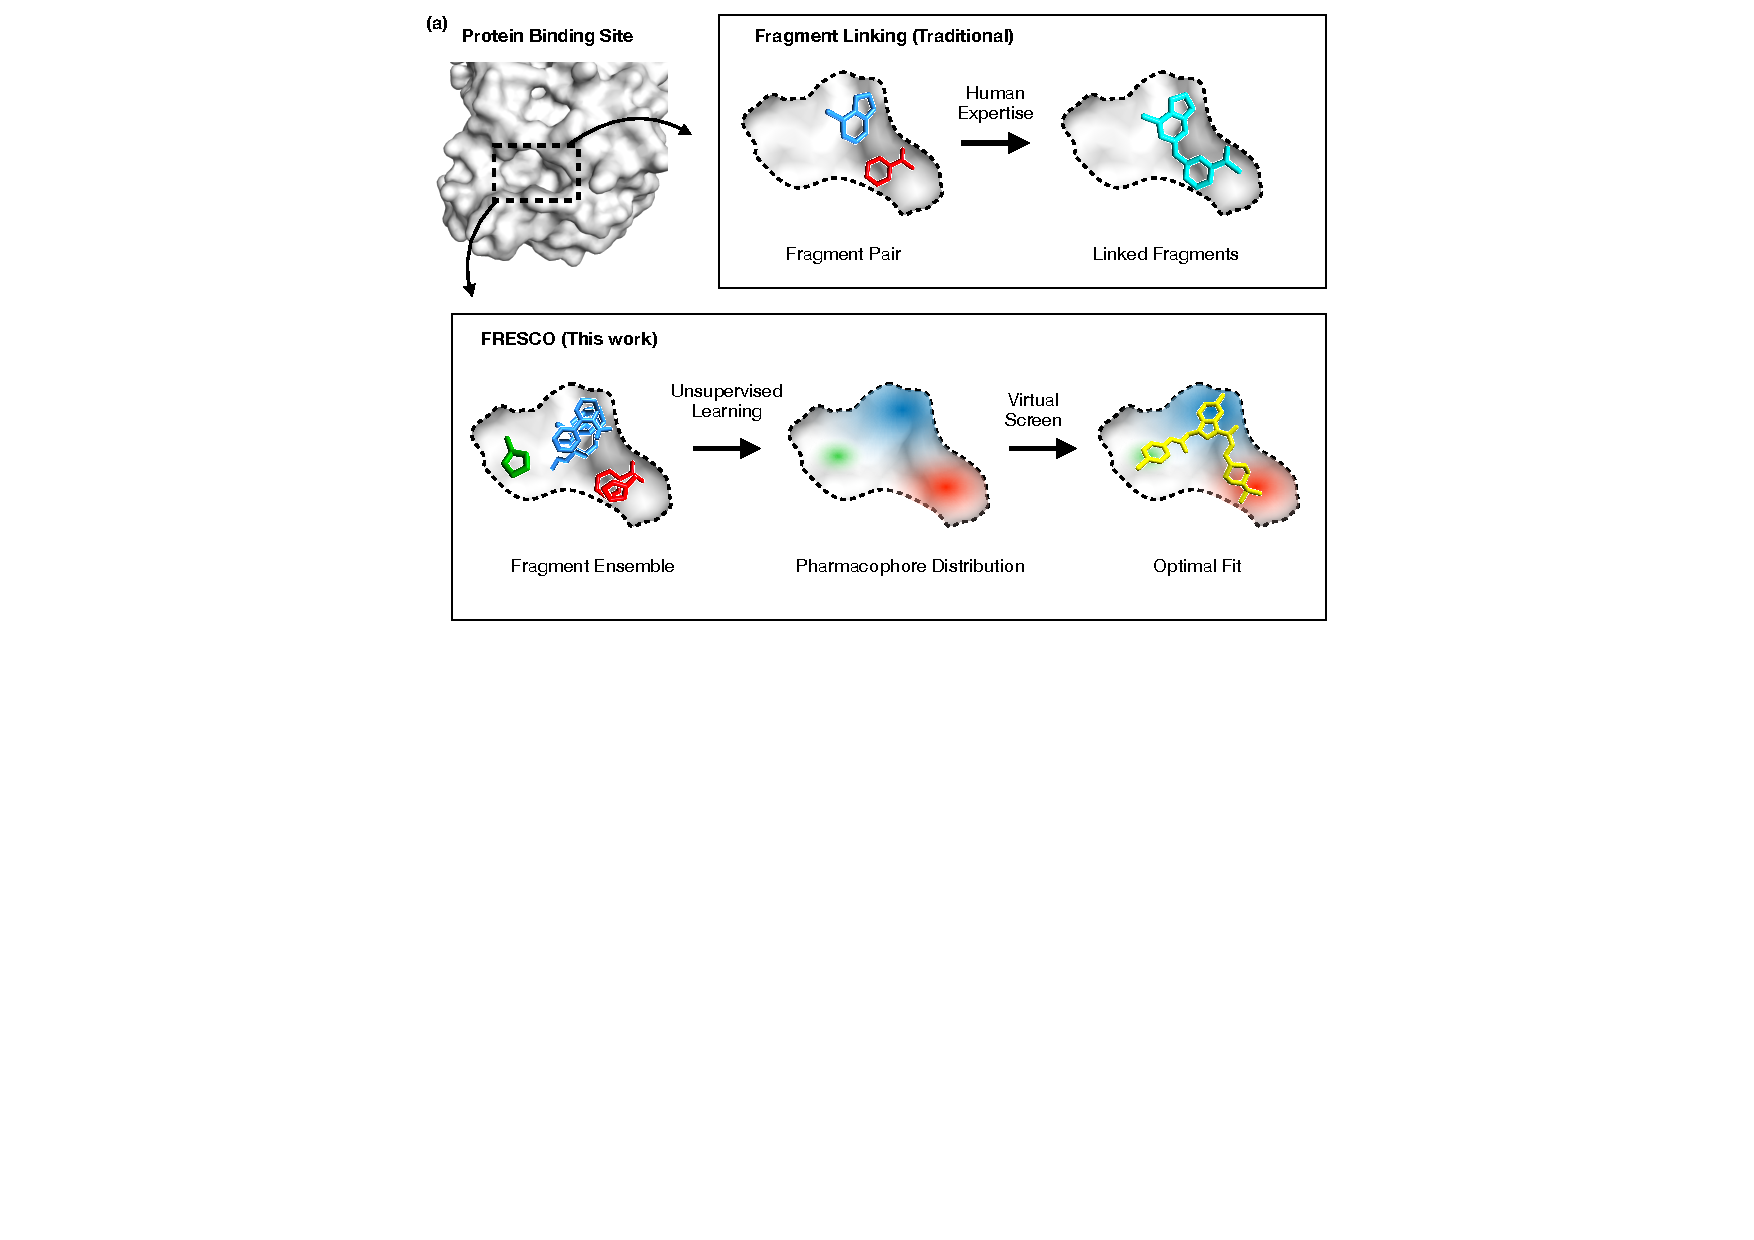
\includegraphics[width=0.75\textwidth]{Chapters/Fresco/Figs/fresco_vs_linking_a.pdf}
    
    \end{subfigure}
    \hfill
    \begin{subfigure}{\textwidth}
        \centering
        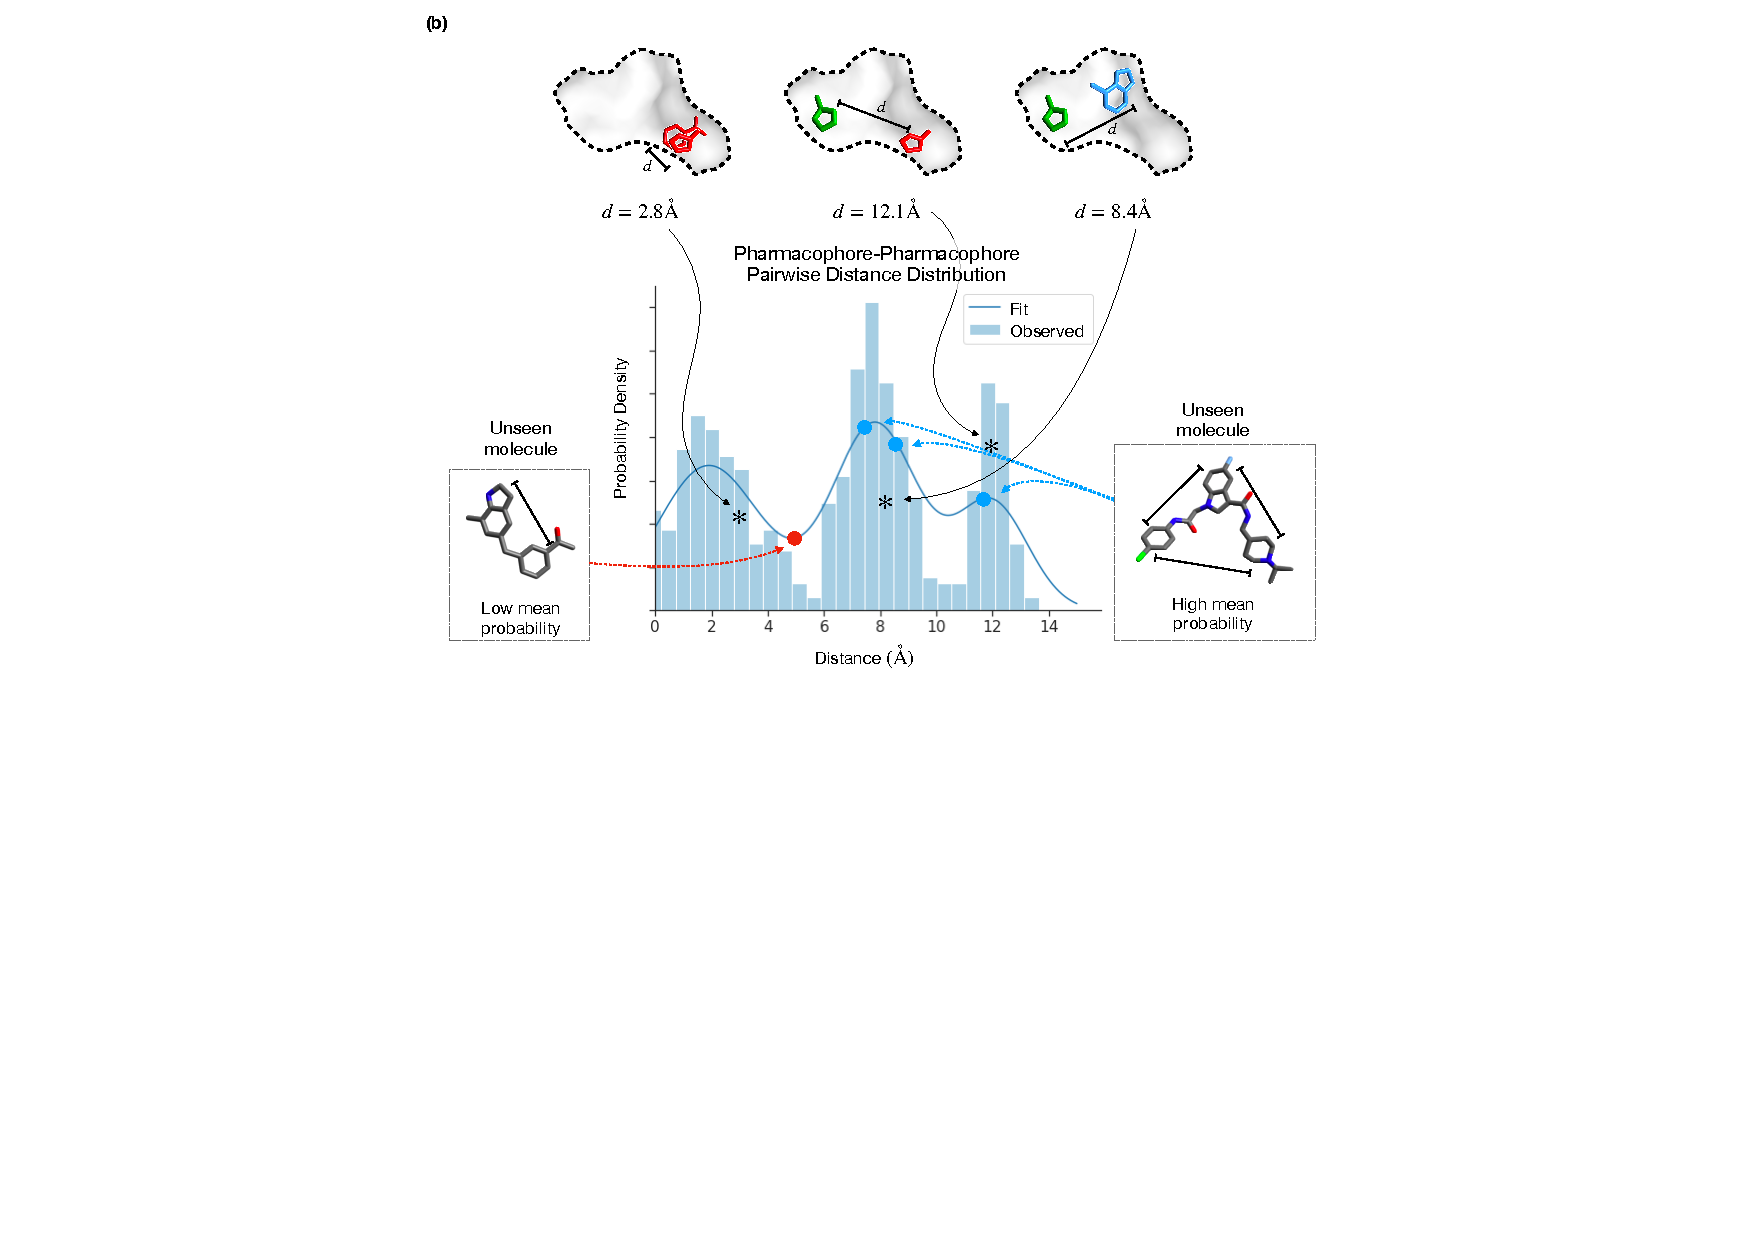
\includegraphics[width=0.75\textwidth]{Chapters/Fresco/Figs/fresco_details.pdf}

    \end{subfigure}
    \caption{(a) A visual illustration of how FRESCO differs from traditional fragment linking approaches. (b) A visual illustration of how we apply unsupervised learning to fragment ensembles and perform virtual screening of unseen molecules.}
    \label{fig:fresco_vs_linking}
\end{figure}

\section{Unsupervised Learning of Pharmacophore Distributions} \label{sec:model}

\begin{figure}[th]
    \centering
    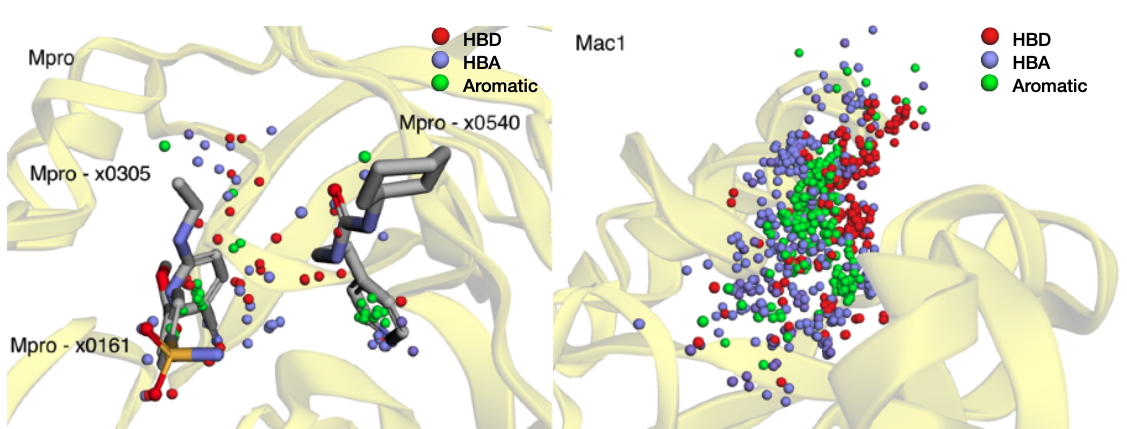
\includegraphics[width=0.8\textwidth]{Chapters/Fresco/Figs/pharmacophores.png}
    \caption{The pharmacophores of the fragment ensemble shown in the 3D binding sites of (a) Mpro, and (b) nsp3-Mac1. The red, blue, and green spheres depict hydrogen bond donors, acceptors, and aromatic pharmacophores respectively. Several of the Mpro fragments are drawn to illustrate the ‘origin’ of some pharmacophores. None are drawn for nsp3-Mac1 due to the density of pharmacophores in the binding site.}
    \label{fig:pharmacophores}
\end{figure}


To turn fragment hits into a model that predicts whether an unknown ligand will bind potently to the binding site, we employ an interpretation inspired by statistical physics. There are multiple chemical motifs that can engage residues on the binding site. These different modes of engagement can be considered as a statistical distribution. Each interaction between a chemical motif on the fragment and a binding site residue corresponds to an instance of this statistical distribution. We assume that the fragment library broadly covers chemical space, and anticipate that stronger interactions will be sampled and therefore observed more often amongst fragment hits than weaker interactions. Note that an individual fragment is a weak binder -- fragment screens are done at a high concentration which forces the equilibrium towards forming fragment-protein complexes enabling detection via crystallography. Therefore, we analyse the statistical distribution of fragment-protein interactions formed by the dense fragment hits, rather than any individual fragment (Figure \ref{fig:fresco_vs_linking}a).

To numerically approximate this distribution, we quantify binding interactions by coarse-graining the fragment molecules into hydrogen-bond donor, hydrogen-bond acceptor, and aromatic ring ``pharmacophores'' (Figure \ref{fig:pharmacophores}). These are a simple abstractions of molecular features that can make potent interactions with binding site residues, and is a commonly used tool to interpret the biological activity of ligands \cite{Kaserer2015PharmacophoreReview}. The distribution which we then choose to approximate is the pair-wise distance between these pharmacophores. Computational screening of compounds based on pharmacophore distances is a commonly used technique in medicinal chemistry, though here we are extending this concept to enable a statistical interpretation of fragment hit. We consider pharmacophore features, rather than specific protein-ligand interactions, so that the downstream model takes the ligand as the input rather than having to perform the additional step of computationally placing the ligand in the binding site. 

%in fragment-based hit dis intention of replicating the intuition of a medicinal chemist deducing spatial correlations between pharmacophores from different fragments.

We utilise kernel density estimation (KDE) \cite{Parzen1962KDE} to estimate this spatial distribution of pair-wise pharmacophore distances. We then score unseen molecules by evaluating pharmacophore distances within that molecule against the probability distribution of pharmacophore distances derived from the fragment ensemble (Figure \ref{fig:fresco_vs_linking}b). We take the mean probability over all of the distances between all possible pharmacophore-pharmacophore pairs as the score for the molecule. This is an unsupervised approach -- starting from the results of a crystallographic fragment screen, without any bioactivity data, we can build a model that computationally screens unseen molecules. We term our approach Fragment Ensemble Scoring (FRESCO). 

FRESCO conceptually departs from machine learning approaches in the literature for fragment-based hit discovery. These approaches, such as DeLinker \cite{Imrie2020DeLinker},  SyntaLinker \cite{Yang2020SyntaLinker}, and Develop \cite{Imrie2021Develop}), as well as data-mining methods such as Fragment Network \cite{Hall2017FragNet}, attempt to grow single fragments or merge only a pair of fragments. They all require expert insights in choosing which fragments to merge, or what pharmacophoric constraints need to obeyed, instead of leveraging all of the information from an ensemble of fragment hits in a data-driven manner.

FRESCO also closes a gap in the burgeoning literature on machine learning for bioactivity prediction \cite{muratov2020qsar}. These models cannot be used when no training data exists, as is the case in the hit-finding phase. Thus a new modelling approach -- here we employed unsupervised learning -- is needed to tackle the ``zero-to-one'' problem. Although physics-based model of ligand-protein binding such as docking \cite{Lyu2019UltraLargeDocking, Alon2021sigma, Fink2022Alpha} can be used in the absence of any bioactivity data, FRESCO crucially incorporates information from the fragment screen on preferential interactions between regions of the binding site and the fragment pharmacophores.

We validate our approach by performing a retrospective study on historical data, as well as embarking on prospectively campaigns on two different protein targets. Retrospective tests or benchmarks, typically the only method used to compare machine learning models, are insufficient for measuring the impact of incorporating the model in the decision-making process of compound selection in drug discovery \cite{Kearnes2021Prospective}. Thus we go beyond typical model development and undertake a prospective search for hit molecules using only FRESCO to obtain a more realistic measure of its performance.

\subsection{Model Implementation} \label{subsec:model_construction}

To train our model, we first process a set of experimental fragment-protein complexes. In this particular work, we downloaded structures from the \href{https://fragalysis.diamond.ac.uk/viewer/react/landing}{\texttt{Fragalysis}} platform \cite{Douangamath2020XChem}. For Mpro, non-covalent fragments from the XChem fragment screen \cite{Douangamath2020XChem} were used while for Mac1 both XChem and UCSF fragment data were used \cite{Schuller2021Mac1Frag}.

We then extract the pharmacophore features from the fragment molecules and their corresponding conformer coordinates. Specifically, we used SMARTS pattern matching following default pharmacophore definitions in \href{https://www.rdkit.org/docs/index.html}{\texttt{RDKit}} to extract pharmacophores from the fragment SMILES. The pharmacophores considered are hydrogen bond donors, hydrogen bond acceptors, and aromatic rings. The corresponding coordinates for each pharmacophore are defined as the average over the atoms in the pharmacophore (eg the position of an aromatic pharmacophore from a benzene ring would be the mean of the coordinates of the 6 carbon atoms in the ring). We then compute the pairwise distance matrix between all possible pharmacophore pairs (eg Donor-Donor \& Aromatic-Acceptor) between different fragment molecules.

For some fragments, multiple crystallographic poses are recorded. To account for this, we weigh the contribution of each fragment structure to the overall fragment pharmacophore distribution by $\frac{1}{n}$ where $n$ is the number of conformations recorded for each conformer. In addition, we exclude the counting of correlations between pharmacophores from the same fragment - only correlations between different fragments are measured. This is to avoid spurious intra-fragment correlations that are unrelated to binding to the binding site - strong correlations in pharmacophore distribution between multiple independent fragments are indicative of useful binding interactions and these are what we hope to capture with this methodology.

With the processed 3D pharmacophore distributions, we can then fit a FRESCO model by learning the probability distribution of the pairwise distances using kernel density estimation (KDE). The bandwidth for KDE fitting was chosen for each pariwise distribution using the Improved Sheather-Jones algorithm \cite{Botev2010ISJ} (implemented in \href{https://kdepy.readthedocs.io/en/latest/index.html}{\texttt{KDEpy}}). KDEs of the systems are then constructed using the chosen bandwidths with \href{https://scikit-learn.org/stable/}{\texttt{scikit-learn}} for technical ease of use in evaluating probabilities. The \texttt{scikit-learn} implementation relies on a relatively slow tree-based algorithm that searches over the training datapoints - to increase the computational efficiency of inference for virtual screening, computationally fast approximations of the KDEs are made using the \texttt{scipy} \href{https://docs.scipy.org/doc/scipy/reference/generated/scipy.interpolate.interp1d.html#scipy.interpolate.interp1d}{\texttt{interp1d}} function.

With a trained FRESCO model, we can then score unseen molecules by evaluating the probability of the pharmacophore distribution of each molecule. Given a set of input molecular conformers (eg from docking), the same processing workflow is used to obtain the 3D pharmacophore distributions of each molecule, and the probability of the distributions are evaluated using the KDEs. The overall score for the molecule is returned as the mean log-probability over all of the pairwise pharmacophore combinations.

\section{Computational Retrospective Study} \label{sec:retrospective}

To validate FRESCO, we evaluate how our method compares against the computational approach of docking, as well as the human expertise of medicinal chemists. Specifically, we wish to estimate the extent to which FRESCO could have accelerated hit identification in a fragment-based drug discovery campaign. This requires a dataset that is explicitly exhibiting structure-activity data from the fragment-to-lead phase of a campaign to accurately reflect the degree of structural diversity and distribution of molecular activity. Use of data from an early-stage high-throughput screen would exaggerate the diversity of structures explored, while data from the lead-optimisation phase of a campaign would artificially contain many potent molecules.

For this reason, we choose to study the COVID Moonshot campaign \cite{Moonshot2022} which is targeting the SARS-CoV-2 main protease (Mpro). Mpro is a target of interest for antiviral drug design as inhibition of Mpro inhibits viral replication, as shown by the recent clinical successes of Paxlovid and Ensitrelvir \cite{Dafydd2021Paxlovid,unoh2022discovery}. COVID Moonshot is, to our knowledge, the only openly available dataset of fragment-to-lead drug discovery, driven by a community of medicinal chemists, where every structure and associated activity is disclosed. This unique dataset allows us to perform a time-split analysis, focusing on the fragment-to-lead phase.

The Moonshot activity data for the retrospective study was accessed in Mar 22nd 2021. The IC50 values in that dataset, as well as in the prospective study on Mpro were measured from a fluorescence based enzyme activity assay, the details of which are described below. To narrow down the data to moleucles during the fragment-to-lead stage of the Moonshot campaign, we only selected molecules which were designed before September 1st, 2020, which gave us a dataset of 979 compounds.

In addition, molecular docking studies have also been done extensively on molecules from the Moonshot campaign \cite{Morris2021Rank, Saar2021biorxiv}. For our analysis we utilise the same docking protocols as those reported previously for consistency, the details of which can be found in the methods section.

In the hit identification phase of drug discovery, relatively little is known about what ligand-protein interactions are feasible, thus most proposed molecules are unlikely to be active. A meaningful metric for comparing methods in this regime is the top-$N$ ``hit rate'', which measures the percentage of the top-$N$ predictions which are active. We expect the curve from plotting the hit rate against $N$ of an informative method to be consistently higher than that of a less informative method. For the Moonshot data we set an IC50 (concentration of inhibitor required to inhibit 50\% of protein activity) threshold of 5\uM for defining a ``hit''. This threshold is relatively arbitrary and repeated analysis for both lower and higher IC50 thresholds (1-15\uM) show similar results.

The baseline hit rate in the dataset i.e. the percentage of compounds with IC50 $<$ 5\uM, is 6.0\%. This represents the hit rate of medicinal chemists using traditional and computational tools at their disposal to design compounds for the Moonshot drug discovery campaign. The hit rate for docking is computed by choosing the top-$N$ molecules with the best score. To calculate the hit rate for FRESCO, we first fit a FRESCO model on 23 publicly reported crystallographic structures of non-covalent fragments bound to the SARS-CoV-2 Mpro protein \cite{Douangamath2020XChem} and score the whole dataset using the fitted FRESCO model.

\begin{figure}[th]
    \centering
    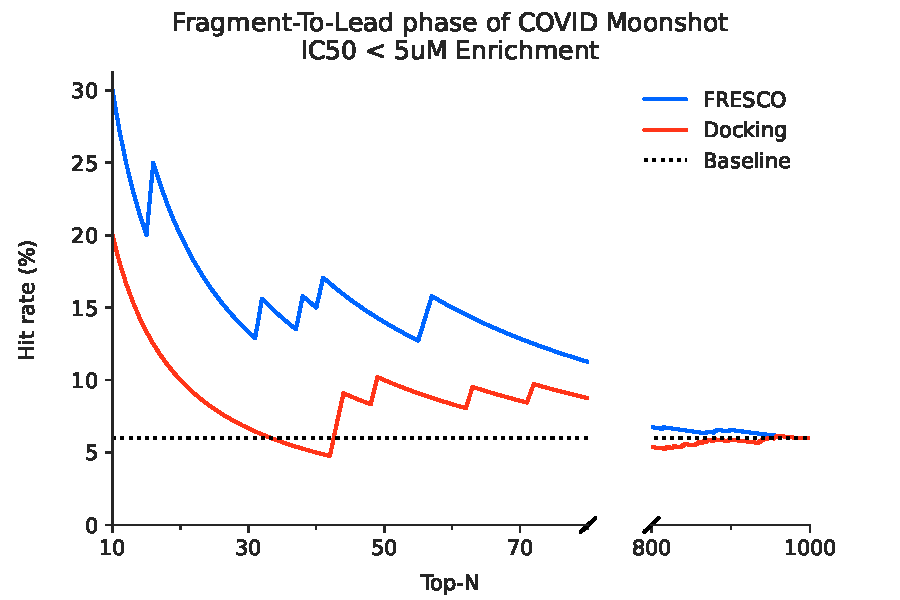
\includegraphics[width=0.8\textwidth]{Chapters/Fresco/Figs/fresco_vs_moonshot_break_5uM.pdf}
    \caption{\textbf{FRESCO is able to retrospectively perform hit detection.} High hit rates are achieved relative to docking and the human expert baseline when ranking molecules from the fragment-to-lead phase of COVID Moonshot.}
    \label{fig:moonshot_enrichment_vs_docking}
\end{figure}

Figure \ref{fig:moonshot_enrichment_vs_docking} shows that FRESCO achieves higher hit rates compared to both computational docking and the medicinal chemists. Looking at the top-5\% of the molecules ($N<50$), FRESCO has a hit rate of 12-30\%, roughly 2-5 times that of the medicinal chemists. Hit rates are also higher than baseline for both lower and higher IC50 thresholds (Figure S3). This shows that it is possible to correlate bioactivity with unsupervised learning of fragment pharmacophore distributions, and that FRESCO could accelerate hit detection in a real-world drug discovery campaign. In this retrospective study, FRESCO is standing on the shoulders of medicinal chemists -- it is used to rescore compounds that are designed by chemists. Therefore, we next turn to interrogate the performance of FRESCO in a real-world context when it is used to score a large unbiased library of compounds via a series of prospective studies. 


\begin{figure}[!h]
    \centering
    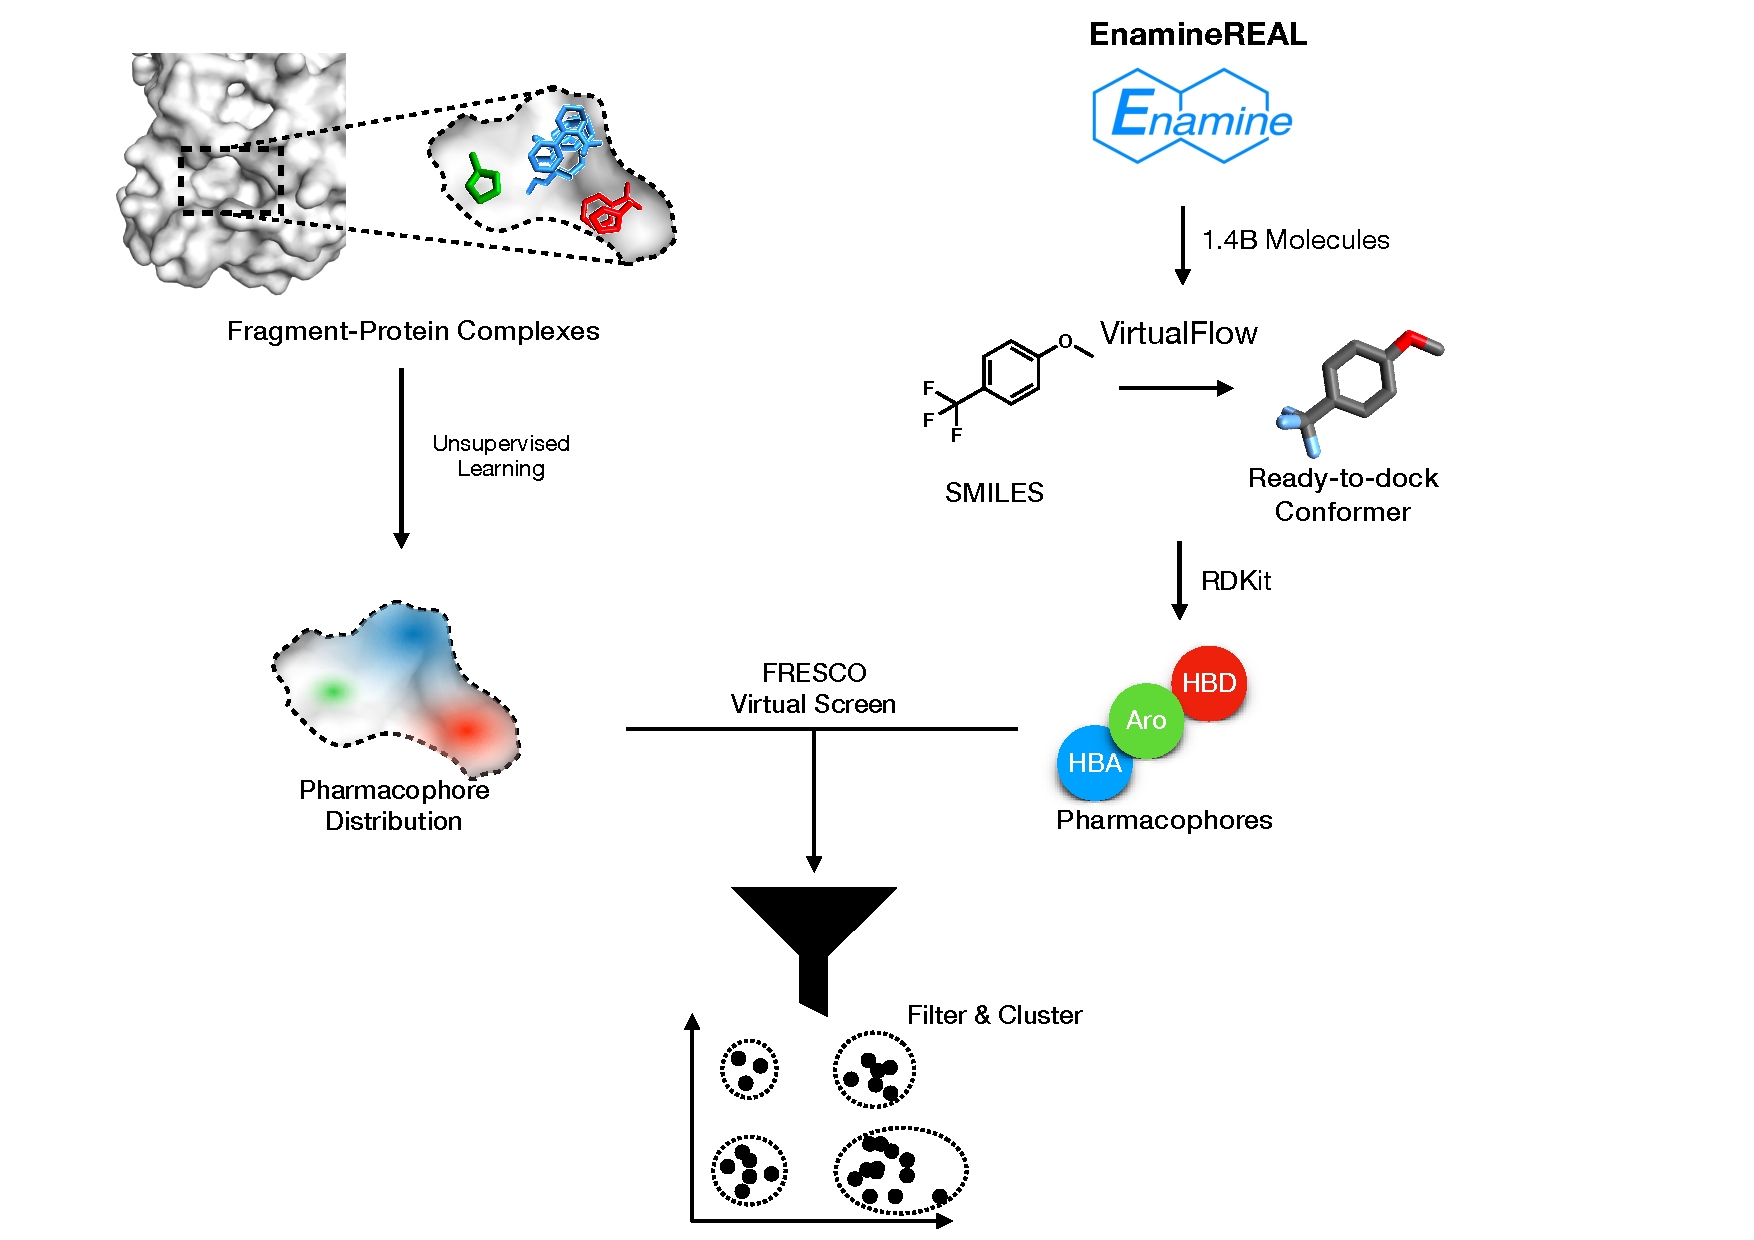
\includegraphics[width=\linewidth]{Chapters/Fresco/Figs/flowchart_screening.pdf}
    \caption{\textbf{A schematic of the FRESCO screening workflow.}}
    \label{fig:screening_workflow}
\end{figure}

\section{Prospective hit finding} \label{sec:prospective}

Building on the results of the retrospective evaluation, we performed a prospective study on Mpro. Rather than rescreening Moonshot compounds, we instead deploy the model to virtually screen a library of commercially available compounds. By synthesising and assaying the top-ranked compounds, we can evaluate the performance of FRESCO in a real-life use case of hit discovery.

The computational workflow we follow to perform the virtual screening is shown in Figure \ref{fig:screening_workflow}. Using a FRESCO model trained on the fragment-protein complexes, we score the library and rank the compounds by score. The top-ranked compounds are then filtered by their physical properties to maximise ``drug-likeness'', and selected diverse compounds by clustered hit by structural similarity and picking centroids of the most populous clusters.


The library we screen is VirtualFlow, a published dataset of more than 1.4 billion commercially available molecules from EnamineREAL \& ZINC15 with pre-generated molecular conformers in a ready-to-dock format \cite{Gorgulla2020VirtualFlow}. The top-500k predictions were selected and filtered to remove undesirable properties. A series of successive filtering steps were performed: first, only molecules with physical properties in well-understood ``lead-like'' chemical space \cite{ChemSpace} were kept. Secondly, the sum of the number of hydrogen bond donors and hydrogen bond acceptors were constrained to an upper limit of 8. Then, we remove molecules that match known filters for pan-assay interference compounds (PAINS) \cite{Baell2010Pains} as well as filters for moieties that are undesirable for medicinal chemistry (eg furan, thiophene, nitro groups). Duplicate tautomers for each molecule are also removed. Finally, for ease of synthetic accessibility, we only consider molecules with less than two chiral centers.

The top-50k molecules remaining from the filtering were then clustered via Butina Clustering \cite{Butina1999Clustering} with a Tanimoto distance threshold of 0.2. This resulted in 24748 for Mpro. The centroids of the 50 most populous clusters (or the closest purchasable analogue if it wasn't available) were chosen as the candidate compounds. These compounds were ordered for synthesis from Enamine which resulted in 38 successfully made molecules.

% This resulted in 24748 and 22358 clusters for Mpro and Mac1, respectively. For both targets the centroids of the 50 most populous clusters (or the closest purchasable analogue if it wasn't available) were chosen as the candidate compounds. These compounds were ordered for synthesis from Enamine which resulted in 38 and 52 successfully made molecules for Mpro and Mac1, respectively.

\begin{figure}[!ph]
    \centering

    \begin{subfigure}{\textwidth}
        \centering
        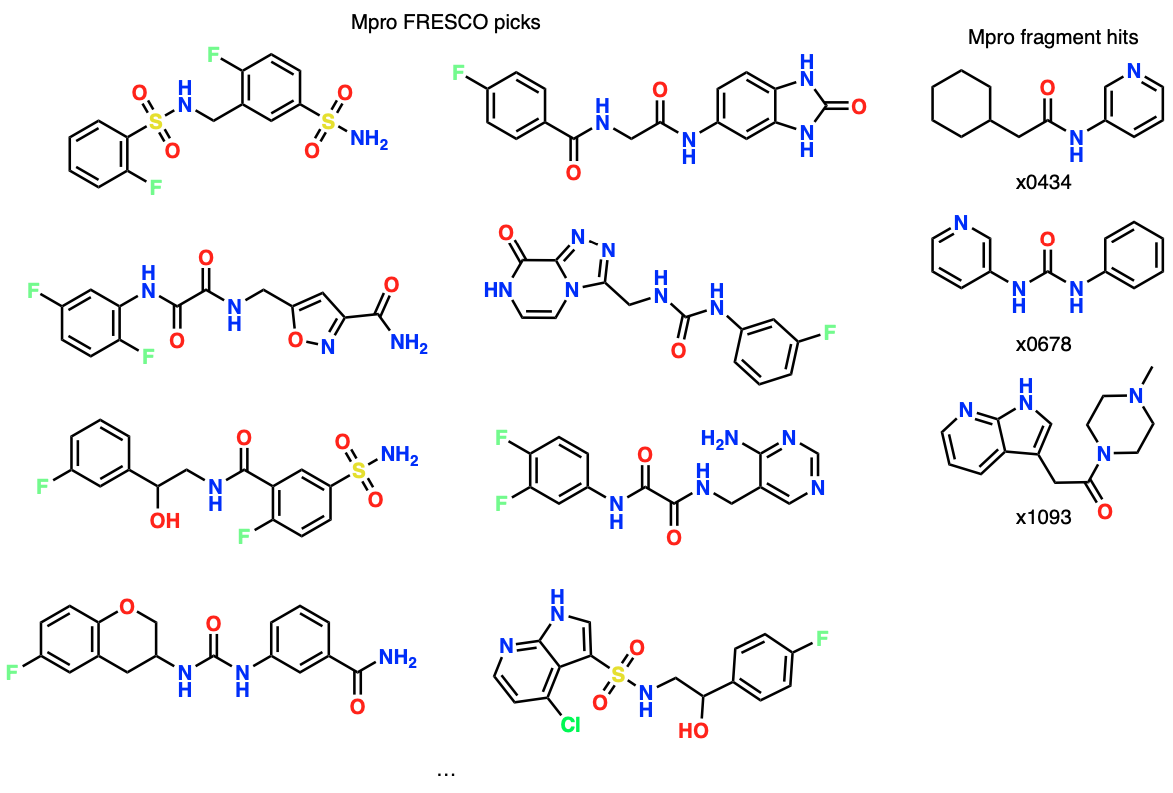
\includegraphics[width=0.75\linewidth]{Chapters/Fresco/Figs/mpro_ligands.png}
        % \caption{(a) Example structures of cluster centroids after executing the FRESCO screening workflow on Mpro. The molecules favoured by FRESCO tend to have 2 aromatic moieties connected via an amide or an amide isostere, similarly exhibited by three of the initial fragment hits whose structures are also shown.}
        % \label{fig:mpro_ligands}
    \end{subfigure}
    \hfill

    \begin{subfigure}{\textwidth}
        \centering
        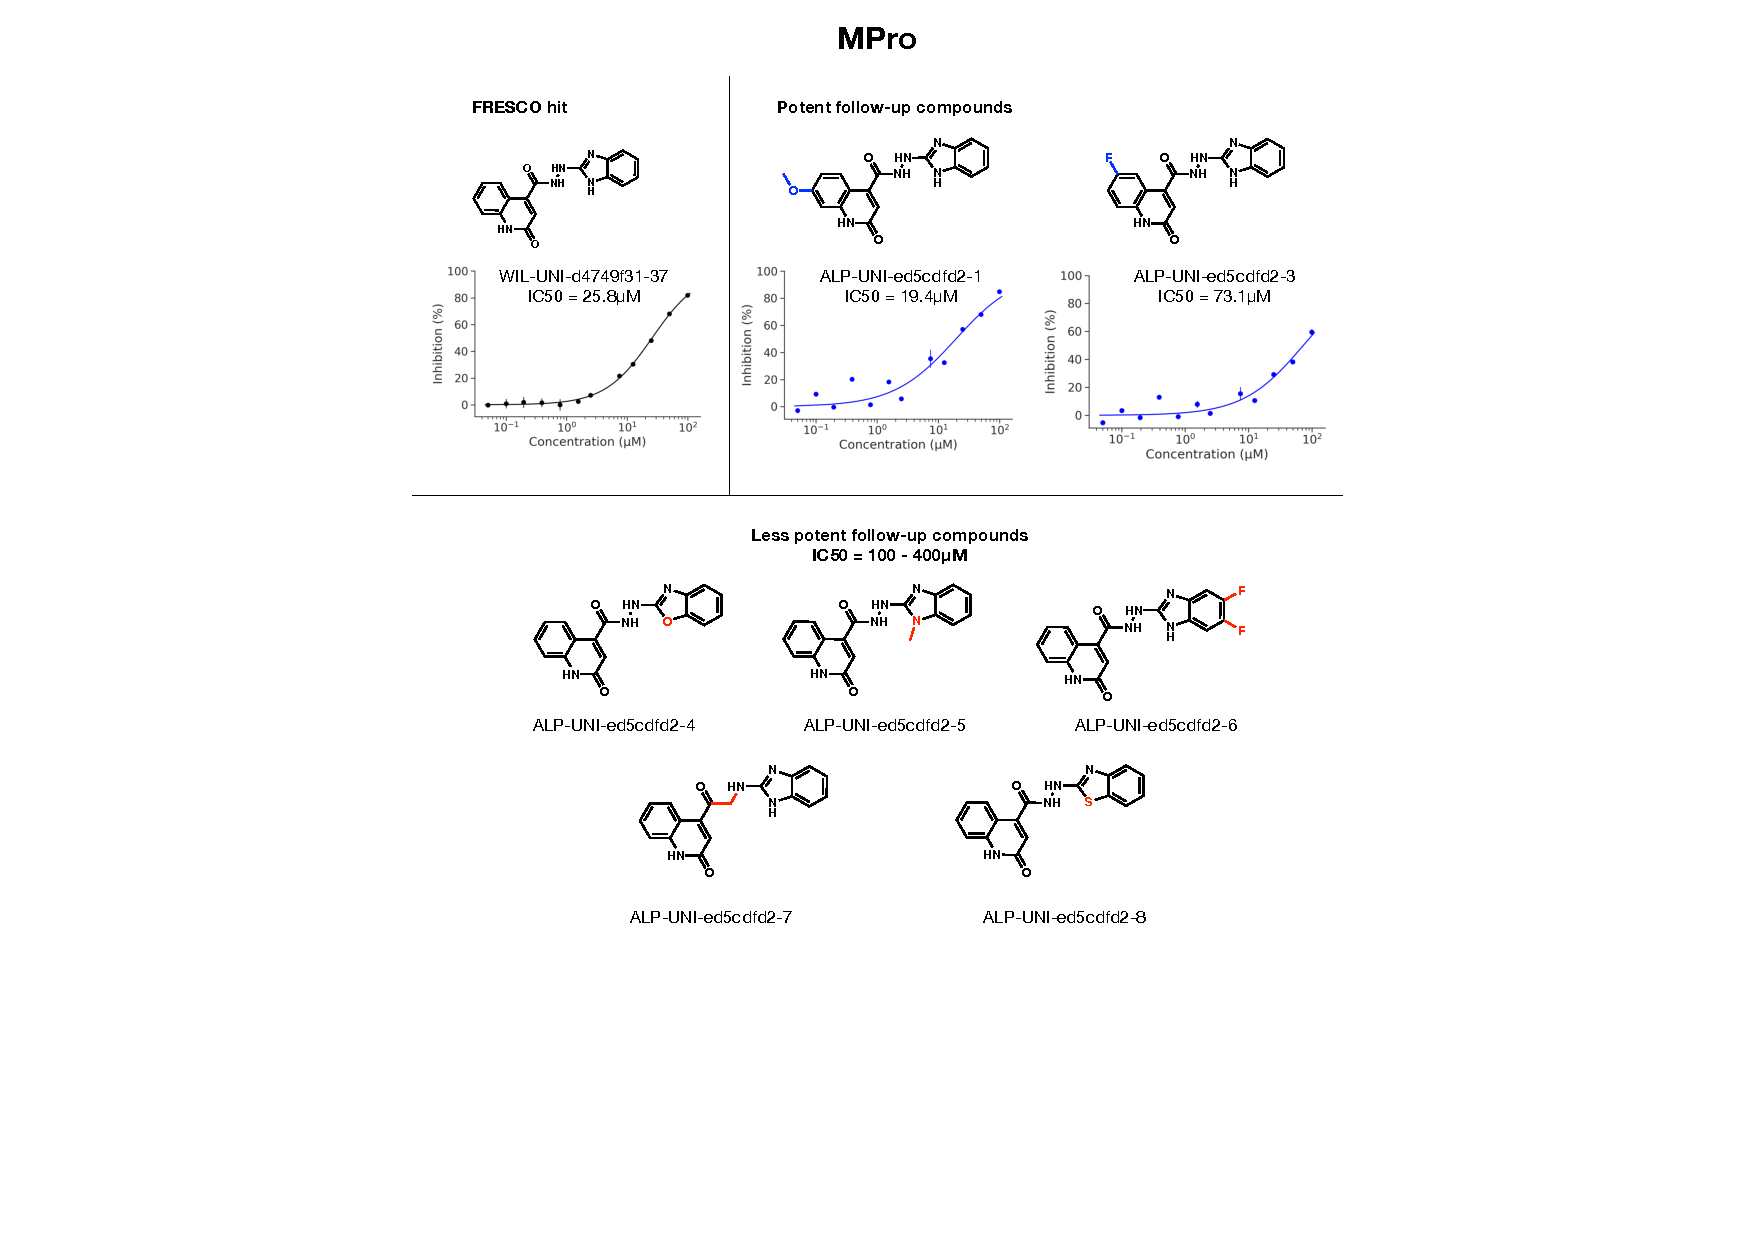
\includegraphics[width=0.75\linewidth]{Chapters/Fresco/Figs/mpro_hit_IC50.pdf}
        % \caption{Compound WIL-UNI-d4749f31-37 is identified as a hit against Mpro, with hit confirmation via follow-up compounds demonstrating SAR. Perturbations to the 2-hydroxyquinoline substructure of WIL-UNI-d4749f31-37 led to increased potency while changes to the benzimidazole group consistently decreased potency. Structural differences between the follow-up compounds and WIL-UNI-d4749f31-37 are highlighted in blue/red.}
        % \label{fig:mpro_hit}
    \end{subfigure}
    \caption{(\textbf{a}) Example structures of cluster centroids after executing the FRESCO screening workflow on Mpro. The molecules favoured by FRESCO tend to have 2 aromatic moieties connected via an amide or an amide isostere, similarly exhibited by three of the initial fragment hits whose structures are also shown. (\textbf{b}) Compound WIL-UNI-d4749f31-37 is identified as a hit against Mpro, with hit confirmation via follow-up compounds demonstrating SAR. Perturbations to the 2-hydroxyquinoline substructure of WIL-UNI-d4749f31-37 led to increased potency while changes to the benzimidazole group consistently decreased potency. Structural differences between the follow-up compounds and WIL-UNI-d4749f31-37 are highlighted in blue/red.}
    \label{fig:mpro_results}
\end{figure}

% \begin{figure}[!hbtp]
%     \centering
%     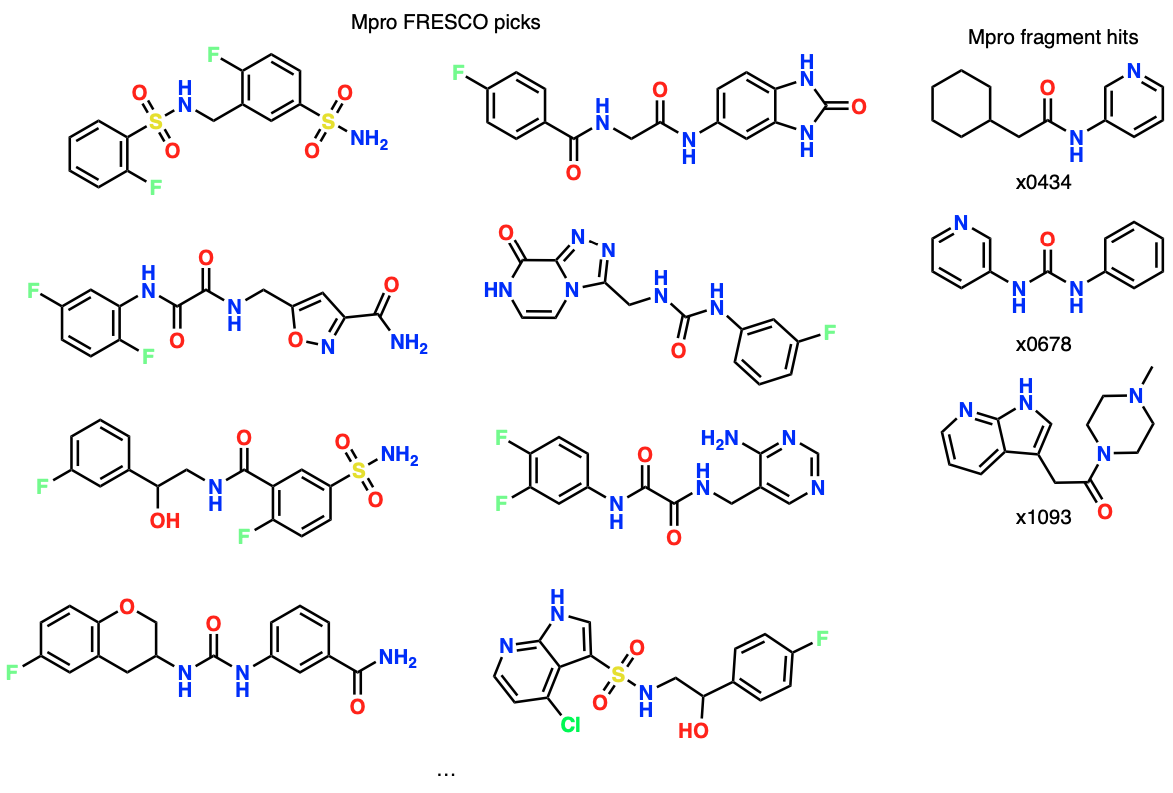
\includegraphics[width=0.75\linewidth]{Chapters/Fresco/Figs/mpro_ligands.png}
%     \label{fig:mpro_ligands}
%     \caption{Example structures of cluster centroids after executing the FRESCO screening workflow on Mpro. The molecules favoured by FRESCO tend to have 2 aromatic moieties connected via an amide or an amide isostere, similarly exhibited by three of the initial fragment hits whose structures are also shown.}
% \end{figure}

% \begin{figure}
%     \centering
%     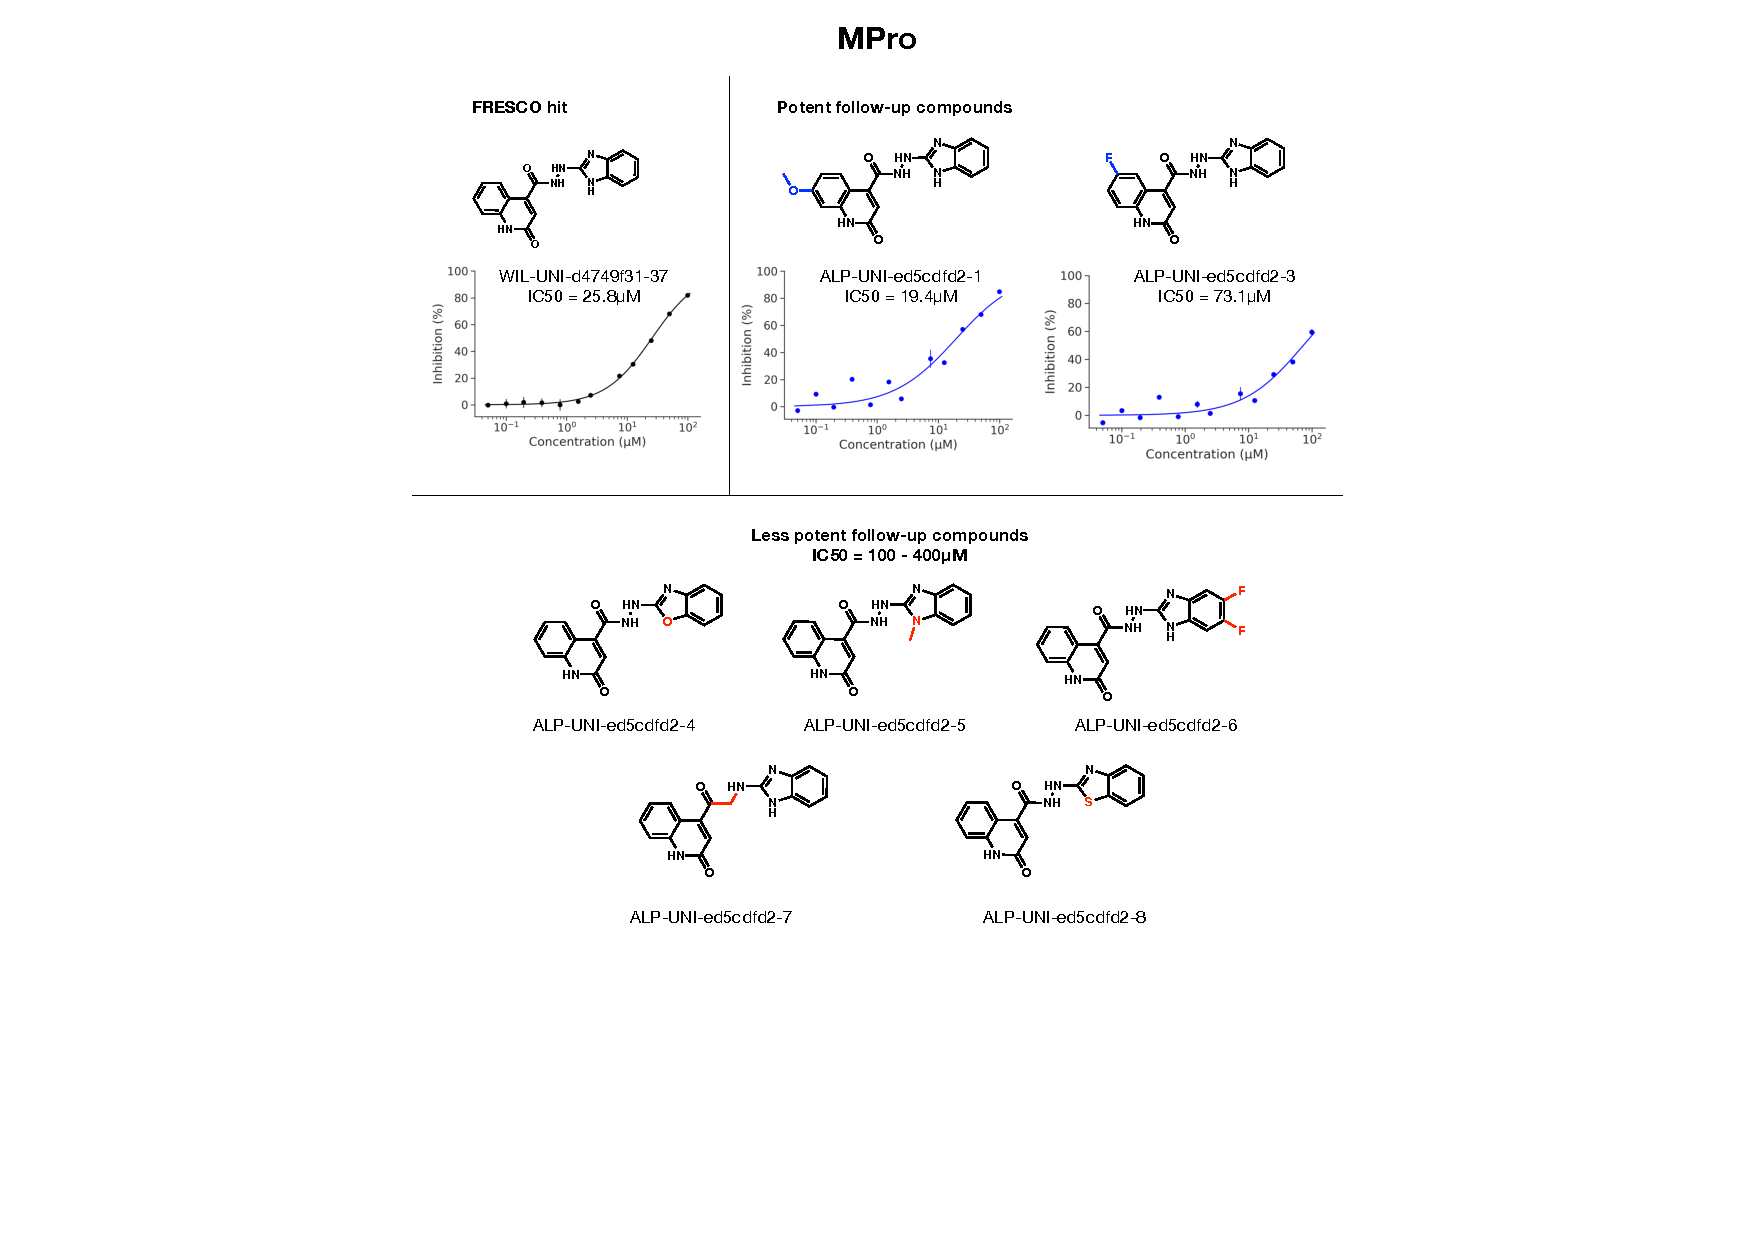
\includegraphics[width=0.75\linewidth]{Chapters/Fresco/Figs/mpro_hit_IC50.pdf}
%     \label{fig:mpro_hit}
%     \caption{Compound WIL-UNI-d4749f31-37 is identified as a hit against Mpro, with hit confirmation via follow-up compounds demonstrating SAR. Perturbations to the 2-hydroxyquinoline substructure of WIL-UNI-d4749f31-37 led to increased potency while changes to the benzimidazole group consistently decreased potency. Structural differences between the follow-up compounds and WIL-UNI-d4749f31-37 are highlighted in blue/red.}
% \end{figure}

Inspecting the cluster centroids favored by FRESCO, we observe typically 2 aromatic moieties connected via an amide or amide isostere. This scaffold is exhibited by three of the initial fragment hits (x0434, x0678, x1093), with the most of the other fragment hits possessing an aromatic group bound at similar locations (Figure \ref{fig:mpro_results}a). The most promising compound, WIL-UNI-d4749f31-37, has an IC50 of 25.8\uM measured via fluorescence assay while the remaining compounds were found to be weak-to-negligible activity.

To validate compound activity, we synthesized 8 close analogues to demonstrate the existence of responsive Structure-Activity Relationship  \cite{Hermann2013ZincImpurity, Morreale2017ZincImpurity} (Figure \ref{fig:mpro_results}b). 3 of those compounds, which contained modifications to the 2-hydroxyquinoline substructure of WIL-UNI-d4749f31-37, retained relatively high potency of IC50 $<$ 100\uM with one of them (ALP-UNI-ed5cdfd2-1) exhibiting a lower IC50 of 19.4\uM. The remaining 5 compounds which perturbed the benzimidazole functional group of WIL-UNI-d4749f31-3 exhibit decreased potency, with only 20-50\% inhibition at a concentration of 99.5\uM.


We then turn to SARS-CoV-2 nsp3-Mac1, a structurally unrelated protein target, to demonstrate generalisability of FRESCO in performing hit detection. nsp3-Mac1 is a viral ADP-ribosylhydrolase which counteracts host immune response by cleaving ADP-ribose that is transferred to viral proteins by host ADP-ribosyltransferases. Unlike Mpro, there is no potent chemical matter against nsp3-Mac1. As such, this is a novel first-in-class biological target. 

\begin{figure}[!b]
    \centering
    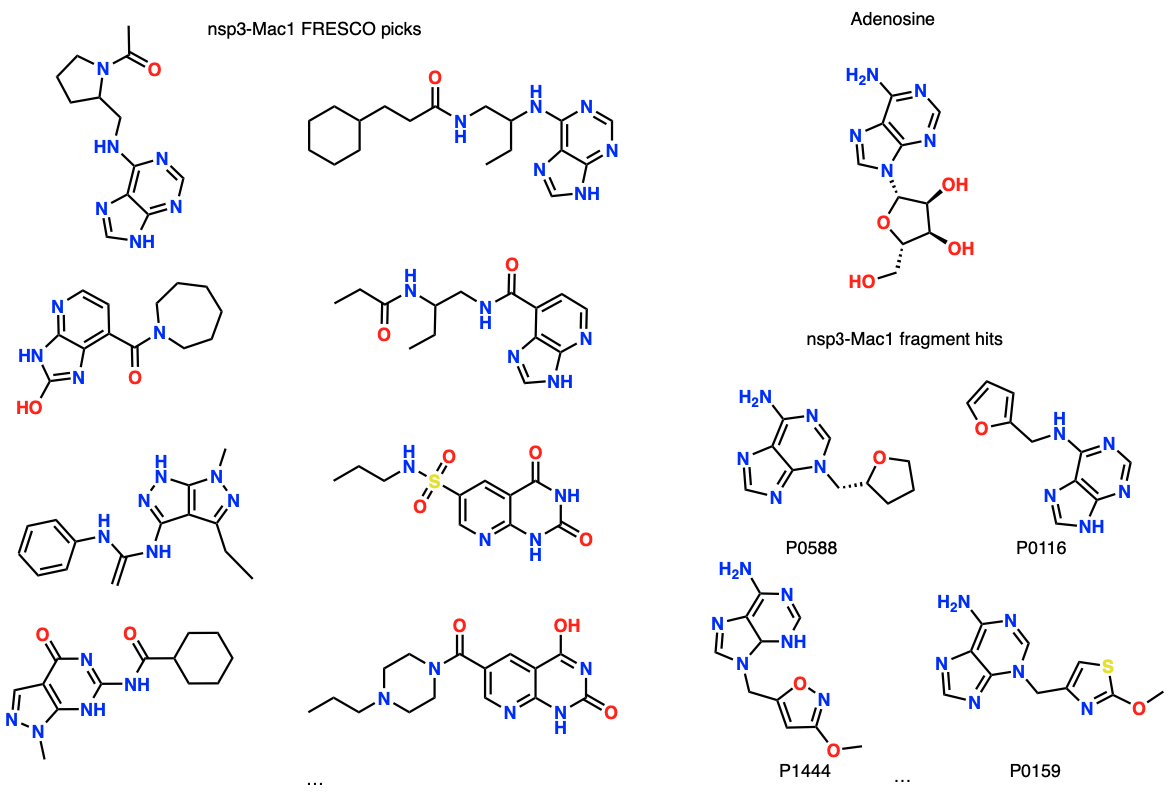
\includegraphics[width=0.8\linewidth]{Chapters/Fresco/Figs/mac1_ligands.png}
    \caption{Example structures of cluster centroids after executing the FRESCO screening workflow on nsp3-Mac1. The molecules favoured by FRESCO tend to contain an acceptor-donor pair spatially proximal to a hetrocyclic motif. This mimics adenosine, a core in the natural substrate.This motif is also shared in many of the initial fragment hits, with some example structures shown in the figure.}
    \label{fig:mac1_ligands}
\end{figure}

Repeating the FRESCO workflow on a fragment screen against Mac1 \cite{Schuller2021Mac1Frag}, we obtained 22358 clusters of top-ranked compounds and successfully made 52 molecules. We find that the molecules favored by FRESCO tend to contain a HBA-HBD pair that is spatially proximal within a hetrocyclic motif. This mimics adenosine, a core in the natural substrate, and this motif is shared in many of the initial fragment hits (Figure \ref{fig:mac1_ligands}). We successfully ordered and assayed 52 of the compounds identified by FRESCO (see SI for the whole library).  Two of the compounds show non-negligible activity at high concentration - at 250\uM, compound Z5551425673 (as a racemic mixture) has an inhibition of 30.1\%, while compound Z1102995175 has 24.8\%.

In addition, an X-ray crystallographic screen was also run on the compounds revealing the structure of Z5551425673 (as the S-stereoisomer) bound to the active site (Figure \ref{fig:mac1_hit}). Crystal structures of 9 other compounds chosen via the FRESCO workflow were also obtained though they did not show notable inhibition via HTRF assay. The orthogonal experimental assay and crystal structure results confirm that Z5551425673 is a hit. 

\begin{figure}[!b]
    \centering
    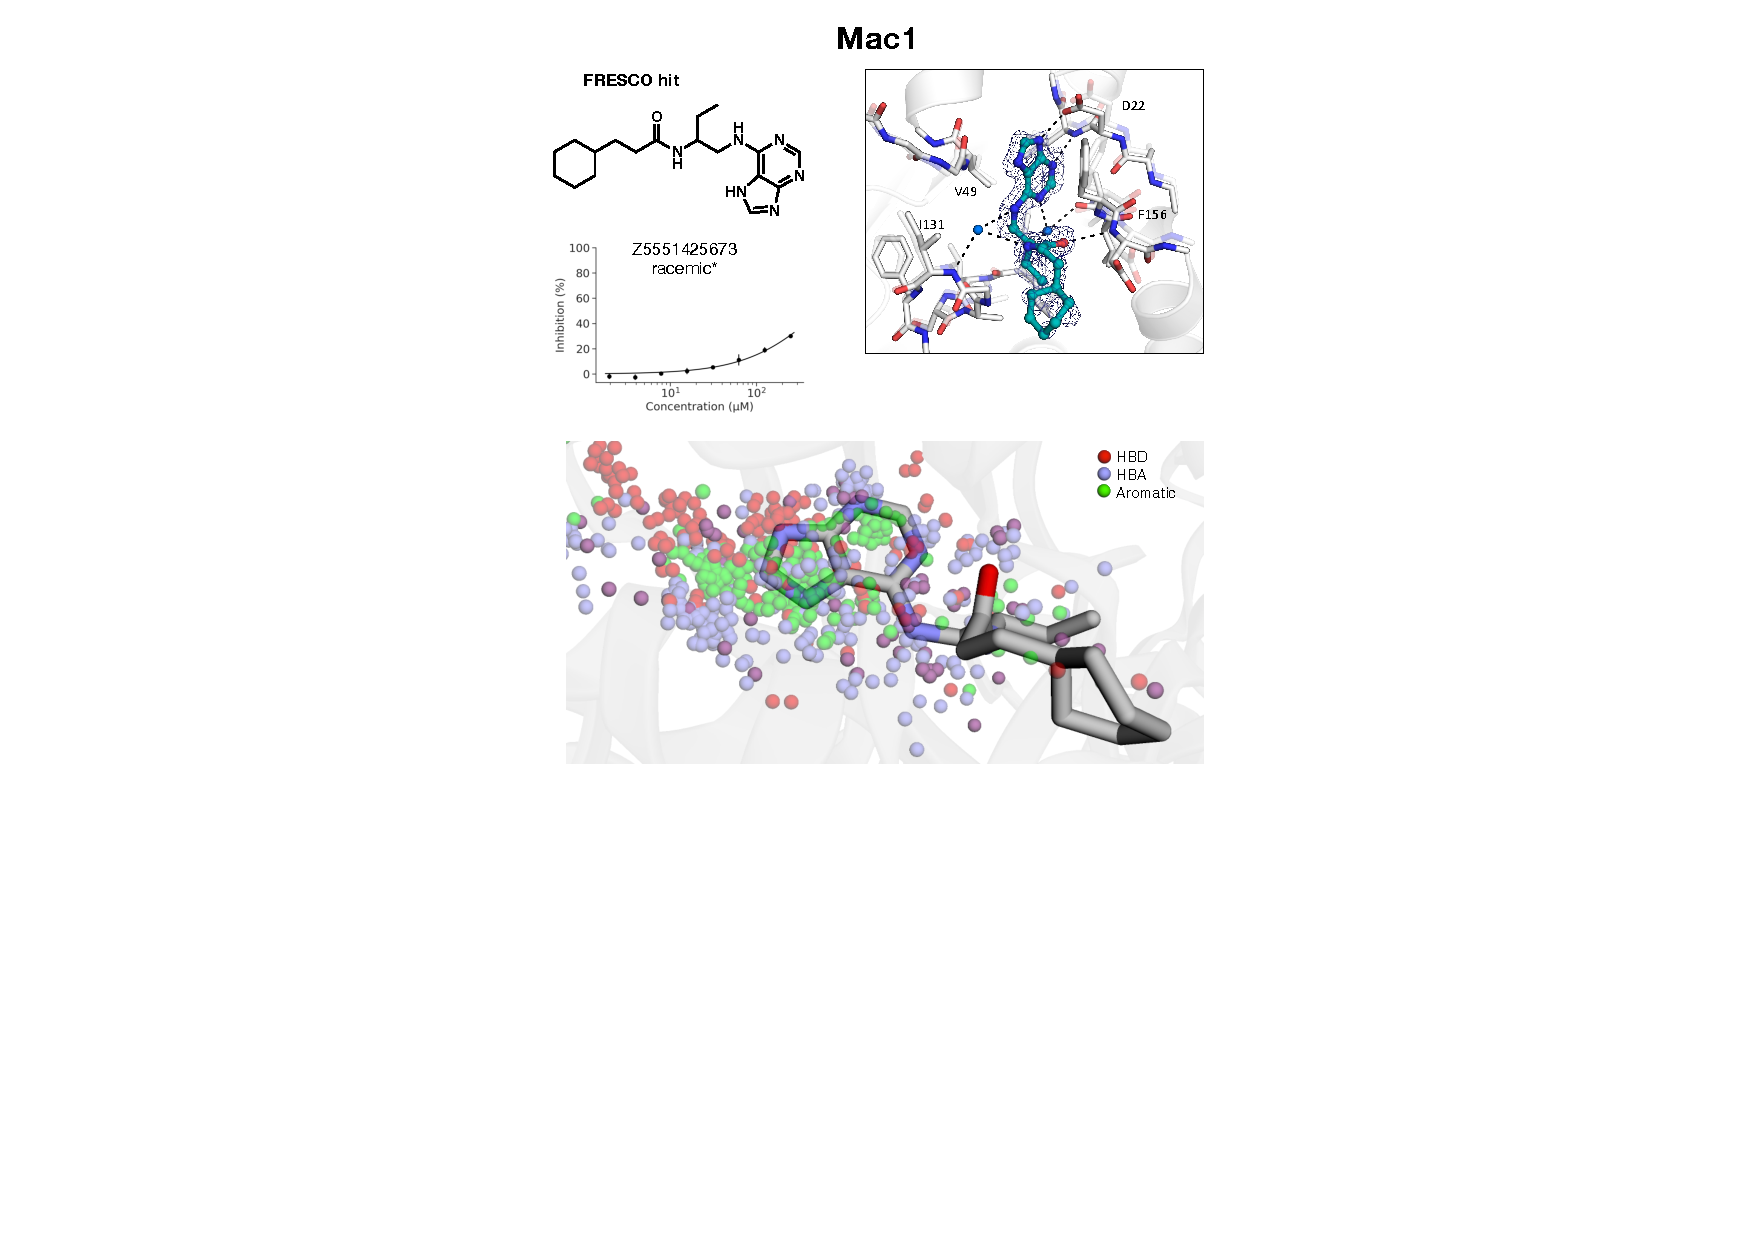
\includegraphics[width=0.75\linewidth]{Chapters/Fresco/Figs/mac1_fig.pdf}
    \caption{(a) Compound Z5551425673 is identified as a hit against Mac1 via HTRF assay, with (b) hit confirmation via resolution of a crystal structure of Z5551425673 (colored in cyan) bound to the Mac1 active site. (c) The pharmacophores of Z5551425673 match those exhibited by the fragment hits as highlighted by overlaying the bound structure of Z5551425673 (PDB 7FR2) on the distribution of pharmacophores from the fragment ensemble. Note that some functional groups can be regarded as both hydrogen-bond acceptor (blue) and hydrogen-bond donor (red) pharmacophores and hence they are illustrated as purple.}
    \label{fig:mac1_hit}
\end{figure}

As with Mpro, 11 close analogues to Z5551425673 were ordered to explore the structure-activity relationship of the hit and ensure that the compound is not a singleton. 4 compounds perturbing the aliphatic tail substructure had relatively negligible effect while the remaining compounds perturbing the purine group led to a large drop in activity (Figure \ref{fig:mac1_rounds}). These sets of molecules, still weak in potency, are potentially promising starting points for a hit expansion campaign. 

\begin{figure}
    \centering
    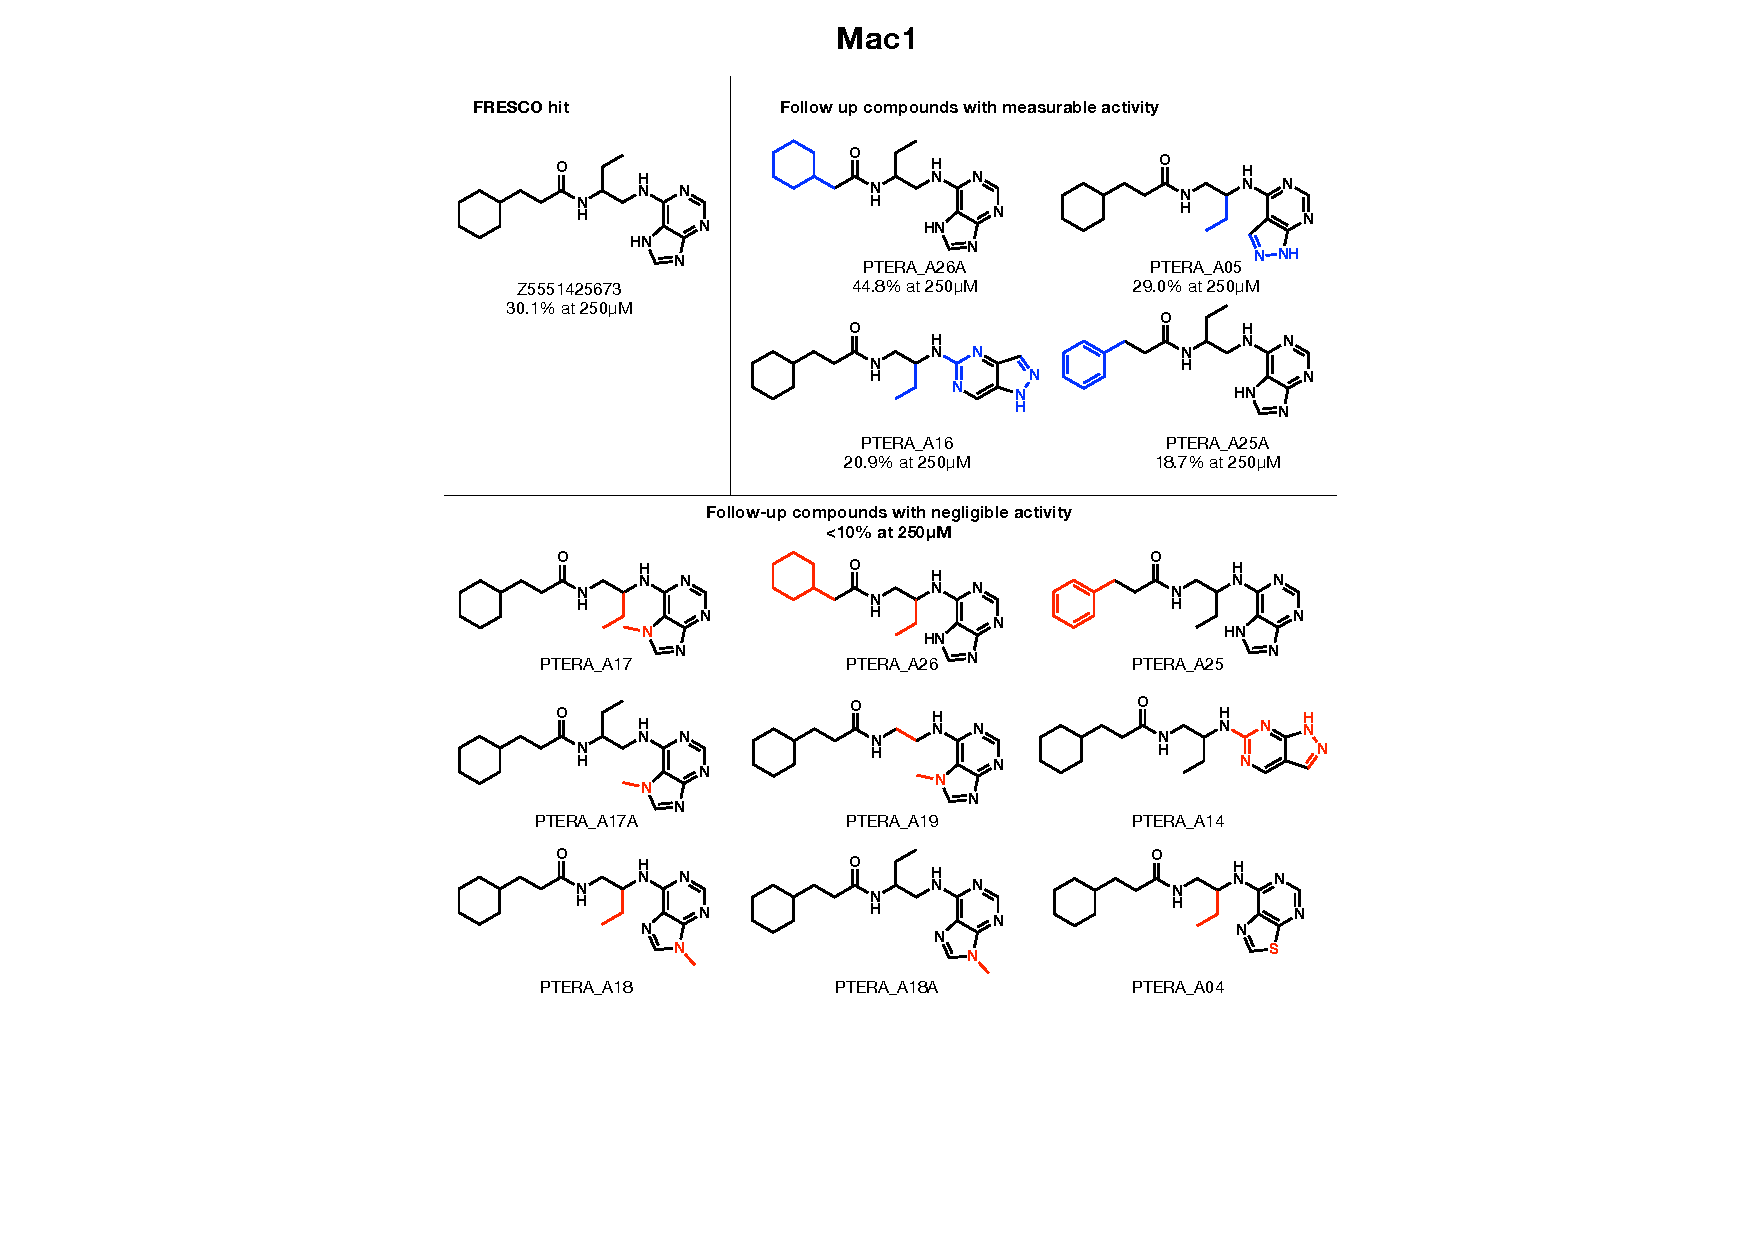
\includegraphics[width=0.75\linewidth]{Chapters/Fresco/Figs/mac1_rounds.pdf}
    \caption{Close analogues around the hit compound identified by FRESCO, Z5551425673, reveals structure-activity relationship which derisks singleton artefacts.}
    \label{fig:mac1_rounds}
\end{figure}


\section{Discussion} \label{sec:fresco_discussion}

Here we show that the combination of computational statistics with high-throughput structural biology and large libraries of purchasable fragment-like molecules unlocks a powerful tool in hit discovery. Going beyond classical fragment-based drug design, which involves merging or expanding a small set of fragments, we derived a statistical framework that leverages dense fragment hits to build potent inhibitors. Whilst individual fragments are weak binders, our key insight is that a fragment-protein interaction is likely to be significant if there are multiple fragments making similar interactions. Therefore, by picking out these persistent interactions, we can discern the salient chemical motifs which make favourable interactions with the binding site. Specifically, we coarse-grained fragments into pharmacophores, and infer the distribution of pairwise distances between pharmacophores using Kernel Density Estimation. We then screen large libraries of purchasable compounds against this fragment-derived pharmacophore distribution. We retrospectively validated our method using data from The COVID Moonshot, an open science drug discovery campaign against the SARS-CoV-2 main protease, and prospectively discovered new hits against SARS-CoV-2 main protease and nsp3-Mac1.

%Although there has been rapid growth in employing machine learning for drug discovery in recent years, particularly in QSAR/molecular property prediction, the vast majority of machine learning approaches are supervised learning techniques. These methods require not merely the existence of experimental assay data, but its existence in sufficient quantity and quality to train a useful model. The nature of the problem of hit detection in early-stage drug discovery is one where such data in nonexistent, which is a fundamental obstacle for applying current techniques. This works shoes how we can instead tap into an underutilised source of rich data by employing unsupervised learning on structural data for affinity prediction. There is already a wealth of crystallographic data available and through collaboration with experimentalists, the field of structural biology can provide a wealth of unique informative unlabelled data for building useful machine learning models for drug discovery.

More generally, we note that our method does not require the observation of affinity data in order to infer potency. This is done by employing an unsupervised machine learning approach on unlabelled structural biology data. As the throughput of structural biology increases, we hope that an unsupervised approach may unlock novel ways of overcoming data limitations in the protein-ligand affinity prediction problem.

Finally, although prospective studies demonstrated FRESCO's ability to identify hits, we note that the hit rate and potency of the identified hits are both lower than the retrospective experiments. This highlights the importance of prospective validation in machine learning -- retrospective studies are biased by the fact that the model is rescoring ``reasonable'' design from medicinal chemists, whereas in prospective evaluations, the model is used to score the large chemical space without further inductive biases. Future efforts to improve FRESCO should seek to include further inductive biases, for example incorporating physics-based constrains such as docking to filter FRESCO outputs, as well as solidifying a human-in-the-loop approach to select top hits. 
\chapter{Discovery of SARS-CoV-2 main protease inhibitors via synthesis-directed de novo design} \label{ch:ranking}

\begin{quote}
 This chapter is based on Aaron Morris, William McCorkindale, The COVID Moonshot Consortium, Nir Drayman, John D. Chodera, Savaş Tay, Nir London, and Alpha A. Lee. Discovery of SARS-CoV-2 main protease inhibitors using a synthesis-directed de novo design model, \textit{Chem. Commun.}, 2021,57, 5909-5912 
\end{quote}

\noindent\hfil\rule{0.5\textwidth}{.4pt}\hfil

% The SARS-CoV-2 main viral protease (Mpro) is an attractive target for antivirals given its distinctiveness from host proteases, essentiality in the viral life cycle, and conservation across coronaviridae. We launched the COVID Moonshot initiative to rapidly develop patent-free antivirals with open science and open data. Here we report the use of machine learning for \emph{de novo} design, coupled with synthesis route prediction, in our campaign. We discover novel chemical scaffolds active in biochemical and live virus assays, synthesized with model-generated routes.

Coronaviruses are a family of pathogens that are frequently associated with serious and highly infectious human diseases, from the common cold to the SARS-CoV pandemic (2003, 774 deaths, 11\% fatality rate), MERS-CoV pandemic (2012, 858 deaths, 34\% fatality rate) and most recently the COVID-19 pandemic (ongoing pandemic, 1.7 million deaths up to Dec 2020).

The main protease (Mpro) is one of the best-characterized drug targets for direct-acting antivirals \cite{pillaiyar2016overview,cannalire2020targeting}. Mpro is essential for viral replication and its binding site is distinct from known human proteases, thus inhibitors are unlikely to be toxic \cite{jin2020structure,liu2020development}. Moreover, the high degree of conservation across different coronaviruses renders Mpro targeting a fruitful avenue towards pan-coronavirus antivirals \cite{ullrich2020sars}. 

% To date, most reported Mpro inhibitors are peptidomimetics, covalent, or both \cite{cannalire2020targeting}. Peptidomimetics are challenging to develop into oral therapeutics, and covalent inhibitors incur additional idiosyncratic toxicity risks. We launched the COVID Moonshot consortium in March 2020, aiming to find oral antivirals against COVID-19 in an open-science, patent-free manner \cite{chodera2020crowdsourcing}. Paxlovid is covalent and peptidomimetic but Pfizer made it orally bioavailable \cite{Dafydd2021Paxlovid}, Ensitrelvir is non-covalent and non-peptidomimetic \cite{unoh2022discovery}.

Here we report the prospective use of algorithmic \emph{de novo} design to rapidly expand hits utilising machine learning (ML) models for ranking compounds by bioactivity as well as synthesis route prediction. Starting from 42 compounds with $\mathrm{IC}_{50}$ within assay dynamic range ($<100 \mu$M) and 515 inactives, our model designed 5 new compounds predicted to have higher activity, together with predicted synthetic routes. All designs were chemically synthesized and experimentally tested, and 3 have measurable activity against Mpro. The top compound has comparable Mpro inhibition to the best in the training set, but with a different scaffold, and is active against the OC43 coronavirus in a live virus assay.

%Describe GenChem 
% Algorithmic \emph{de novo} design aims to automatically generate compounds that are chemically diverse, synthetically accessible, and biologically active \cite{schneider2016novo}. Classic approaches apply heuristics to fragment and modify known active compounds, with the region of chemical space explored and synthetic accessibility constrained by those rules \cite{brown2004graph,patel2009knowledge,hartenfeller2012dogs}. Recent machine learning approaches explore chemical space in more abstract molecular representation space \cite{gomez2018automatic,segler2018generating}, but this often comes at the expense of synthetic accessibility \cite{Gao2020Synthesizability}. Our approach builds on rule-based fragmentation and molecule generation but employs a method that combines regression and classification amid noisy data, and the use of machine learning to predict synthesis routes.

\section{Learning to rank compounds}
Our compound prioritisation model aims to predict whether a designed compound is likely to be an improvement in activity over the incumbent. However, as is typical in the hit-expansion stage, bioactivity modelling is hindered by insufficient data where the majority of compounds are inactive, and noisy data as measurement variability increases for lower affinity compounds. Thresholding the data and framing the problem as classification of active/inactive would not allow us to rank compounds based on predicted improvement over the incumbent, yet the relatively small number of quantitative potency measurement bioactivity data and the measurement noise make a regression approach challenging.

Instead of predicting IC50 values directly, we focused our attention on a learn-to-rank approach \cite{duffy2010molecular,agarwal2010ranking} that predicts the pairwise comparison of ligands - given a pair of molecules $(A, B)$, the model predicts whether $A$ is more active than $B$. This approach allows us to assimilate both coarse (active/inactive) and fine (quantitative potency measurements) data into a single model, effectively combining `easy' classification and `difficult' regression into a `moderate' task of ranking input pairs. With a trained ranking model, we can screen for more potent inhibitors by ranking new molecules against the most potent active compounds in the dataset.

\begin{figure}[!th]
 \centering
 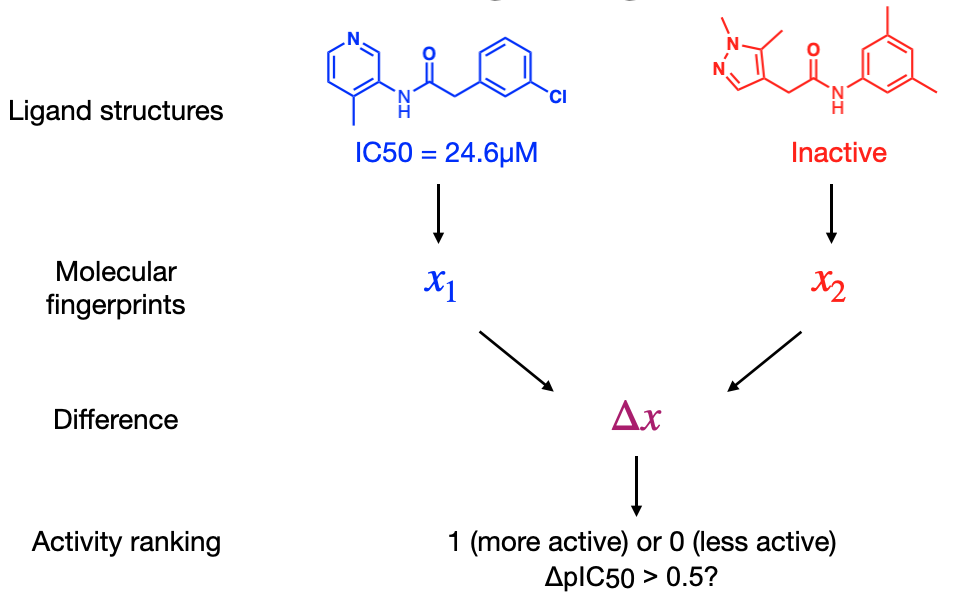
\includegraphics[width=0.85\textwidth]{Chapters/Ranking/Figs/schematic.png}
 \caption{\textbf{A schematic of the model setup.} A classifier takes the difference in molecular fingerprint between two molecules and predicts where one molecule is more or less active than the other.}
 \label{fig:ranking_schematic}
\end{figure}

To implement this ranking model (Figure \ref{fig:ranking_schematic}), we use the difference in molecular fingerprints between two molecules, $f_A - f_B$ as input to the model, and the output is the whether the molecule $A$ is more or less potent than molecule $B$. The descriptor we use for representing a molecule is a concatenation of 3 512-bit fingerprint representations (Morgan, Atom, Topological Torsion) into one 1536 representation. A multilayer perceptron, implemented via the FastAI Tabular framework \cite{howard2018fastai}, is used for modelling the data. The choice of molecular descriptor and model was based on empirical performance (Details on the model implementation can be found in Appendix \ref{appendix:ranking}). %The fingerprint is projected onto 20 dimensions using Principal Component Analysis.

To construct a suitable dataset for training the model, the activity data must be reformated into pairs of molecules. This is done by pairing all actives with all inactives, as well as pairing up actives where there is a significant difference in bioactivity ($\Delta$pIC50 $>0.5$). This threshold was chosen to match typical assay error, forcing the model to ignore irrelevant experimental noise by ensuring that it is ranking only ligands with demonstrably different bioactivity. The inactive molecules were not paired up with each other as the ranking of inactivity is not relevant to the task at hand and potentially noisy/misleading.

\begin{figure}[!th]
 \centering
 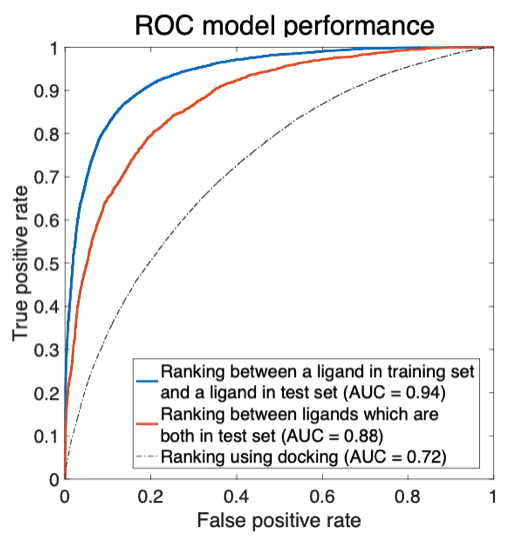
\includegraphics[width=0.65\textwidth]{Chapters/Ranking/Figs/roc_curve.png}
 \caption{\textbf{Relative ranking of ligands can be predicted by our learning-to-rank machine learning model.} The Receiver Operating Characteristic curve of classifying whether a molecule is more/less active than the other.}
 \label{fig:roc_plot}
\end{figure}

A flipped pairing is included for all pairs so that the dataset is antisymmetric since the model would just predict ones otherwise. Theoretically, this method is appealing because it is a natural way of oversampling the low proportion of actives, addressing the problem of dataset imbalance commonly seen in drug discovery classification tasks. Additionally, creating pairs between the actives allows the exploitation of activity information without the noise/difficulty of trying to learn accurate pIC50 values.

% We compare the performance of our model in predicting the pairwise ranking of compounds against the baseline model of simply training a regression model on bioactivities. As a baseline model, we trained a random forest model with the package \texttt{scikit-learn} \cite{scikit-learn}, \texttt{RandomForestRegressor} function, with default hyperparameters. Likewise, for the learning-to-rank model, we employ the FastAI tabular model, a general machine learning package for processing classification problems. 

% \begin{table}[]
% \centering
% \begin{tabular}{|l|l|l|}
% \hline
% \textbf{Dataset} & \textbf{RF Baseline AUC} & \textbf{Model AUC} \\ \hline
% LCK & \textbf{0.94} & 0.91 \\ \hline
% opioid & 0.92 & \textbf{0.94} \\ \hline
% Cannabinoid & \textbf{0.97} & 0.87 \\ \hline
% Estrogen & 0.96 & \textbf{0.98} \\ \hline
% B-raf & 0.95 & \textbf{0.96} \\ \hline
% Ephrin & 0.83 & \textbf{0.85} \\ \hline
% Glycogen & \textbf{0.89} & 0.88 \\ \hline
% Vanilloid & \textbf{0.93} & 0.90 \\ \hline
% JAK2 & 0.97 & \textbf{0.98} \\ \hline
% Dopamine & 0.97 & \textbf{0.98} \\ \hline
% ABL1 & 0.81 & \textbf{0.84} \\ \hline
% A2a & 0.58 & \textbf{0.91} \\ \hline
% Coagulation & 0.82 & \textbf{0.85} \\ \hline
% Glucocorticoid & 0.96 & \textbf{0.98} \\ \hline
% Dihydrofolate & \textbf{0.90} & 0.86 \\ \hline
% Carbonic & 0.97 & \textbf{1.00} \\ \hline
% Aurora-A & 0.89 & \textbf{0.93} \\ \hline
% \end{tabular}
% \caption{Comparing learning-to-rank with direct potency prediction in prioritising compounds.}
% \label{table1}
% \end{table}


For performance evaluation, the dataset was randomly split into training (80\%) and testing (20\%) sets (with roughly the same active/inactive proportion) before the molecules are paired up independently within each set. This ensures that there is no cross-talk between the train/test sets where the model could simply memorize the activity of certain compounds. We train the model on pairs of compounds within the training set and evaluate the model on both pairs within the test set as well as pairs between the training and test set.


Figure \ref{fig:roc_plot} shows that our binary ranking model achieves an AUC of 0.88 (95\% CI: [0.83,0.96]) in ranking ligands within the test set, and an AUC of 0.94 (95\% CI: [0.91,0.98]) where we compare a ligand in the training set against another ligand in the test set; the latter is more relevant as our goal is finding ligands more active than the best incumbent. The 95\% confidence interval is computed using bootstrapping. We also compare our model against ranking compounds using docking scores generated with OpenEye's FRED docking algorithm, which achieves an AUC of 0.72 (95\% CI: [0.722,0.723]) (Details of the docking procedure can be found in Appendix \ref{appendix:docking}). Note that docking does not require ligand bioactivity as training data, thus is not a direct comparison to machine learning.

% In the Supplementary Material, we discuss that our model ranks ligands better than a model that directly learns $\mathrm{IC}_{50}$ (AUC = 0.86; 95\% CI: [0.71,0.95]). 

Beyond train-test split, model performance can be evaluated from a time-split. Five months have elapsed from the time we deployed our model for prospective compound selection to writing up this work. During that time, the COVID Moonshot Consortium (a team of expert medicinal chemists) has independently designed, synthesised, and tested 356 compounds \cite{moonshot2020covid}, out of which 15\% were better than the top 2 compounds (having $\mathrm{IC}_{50}$ comparable within error) in our dataset. Table \ref{table:time_split} shows that our model has an enrichment factor of $\sim$2, i.e. if we re-score the 356 compounds synthesized by the medicinal chemistry team using our model, and pick the top 1\%-10\% percentile, the proportion of molecules that would be better than the top 2 compounds would be $\sim$2x higher than human selection. 

\begin{table}[!bh]
 \centering
 \begin{tabular}{|l|l|l|l|}
 \hline
 \textbf{Percentile} & 1\% & 2.5\% & 10\% \\ \hline
 \textbf{Enrichment Factor} & 1.7 & 2.3 & 1.7 \\ \hline
 \end{tabular}
 \caption{Enrichment factor for the time-split dataset, where we consider model performance on data arriving after the model has been deployed to generate compounds for synthesis and testing. }
 \label{table:time_split}
\end{table}

These retrospective results illustrate that a learning-to-rank approach can leverage bioactivity data from both active and inactive molecules for the enrichment of potent compounds in a real-world drug discovery campaign. In the next section, we deploy our model to discover new Mpro inhibitors in a prospective experiment.

\section{Prospective chemical space exploration}
% Classic approaches apply heuristics to fragment and modify known active compounds, with the region of chemical space explored and synthetic accessibility constrained by those rules \cite{brown2004graph,patel2009knowledge,hartenfeller2012dogs}. Recent machine learning approaches explore chemical space in more abstract molecular representation space \cite{gomez2018automatic,segler2018generating}, but this often comes at the expense of synthetic accessibility \cite{Gao2020Synthesizability}. Our approach builds on rule-based fragmentation and molecule generation,

After designing a well-founded ML scoring model, we must decide on a virtual library of compounds to explore. While one could screen an ultra-large library of make-on-demand compounds as in the previous chapter, it is only feasible for a relatively cheap computational model which is not the case for the neural network-based ML model developed in this work. 

Instead, we consider a more targeted approach by exploring the smaller, local chemical space of chemical substructures contained within our initial dataset. Building on rule-based fragmentation methods such as BRICS \cite{Degen2008brics} and CReM \cite{Polishchuk2020Crem}, our general approach is to decompose the existing molecules into a large set of distinct substructure components before enumerating all components with one another, generating a large number of novel and diverse molecules. 

\begin{figure}[!th]
 \centering
 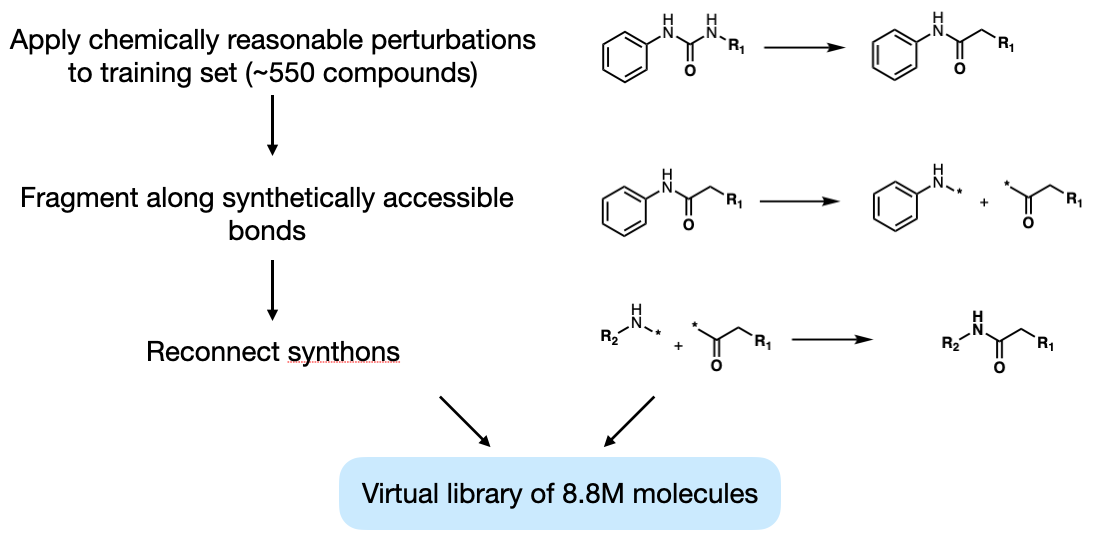
\includegraphics[width=0.75\textwidth]{Chapters/Ranking/Figs/library.png}
 \caption{\textbf{A schematic of the methodology for the library generation process.}}
 \label{fig:library}
\end{figure}

Specifically, we first introduce a set of chemically reasonable perturbations (linker and chemotype swaps, e.g. amide to retroamide, amide to urea, swapping N-aryl groups), which is applied to the whole set of active molecules. We then fragment along synthetically accessible bonds (e.g. amides and aromatic C-C and C-N) and reconnect the synthons to generate an exhaustive library (Figure \ref{fig:library}). These operations are defined using SMARTS rules.

The resulting library of 8.8 million generated molecules is then scored against the top 3 compounds in the training set using the learning-to-rank framework, and the mean score is taken as the final score for each compound.

\begin{figure}[!bh]
 \centering
 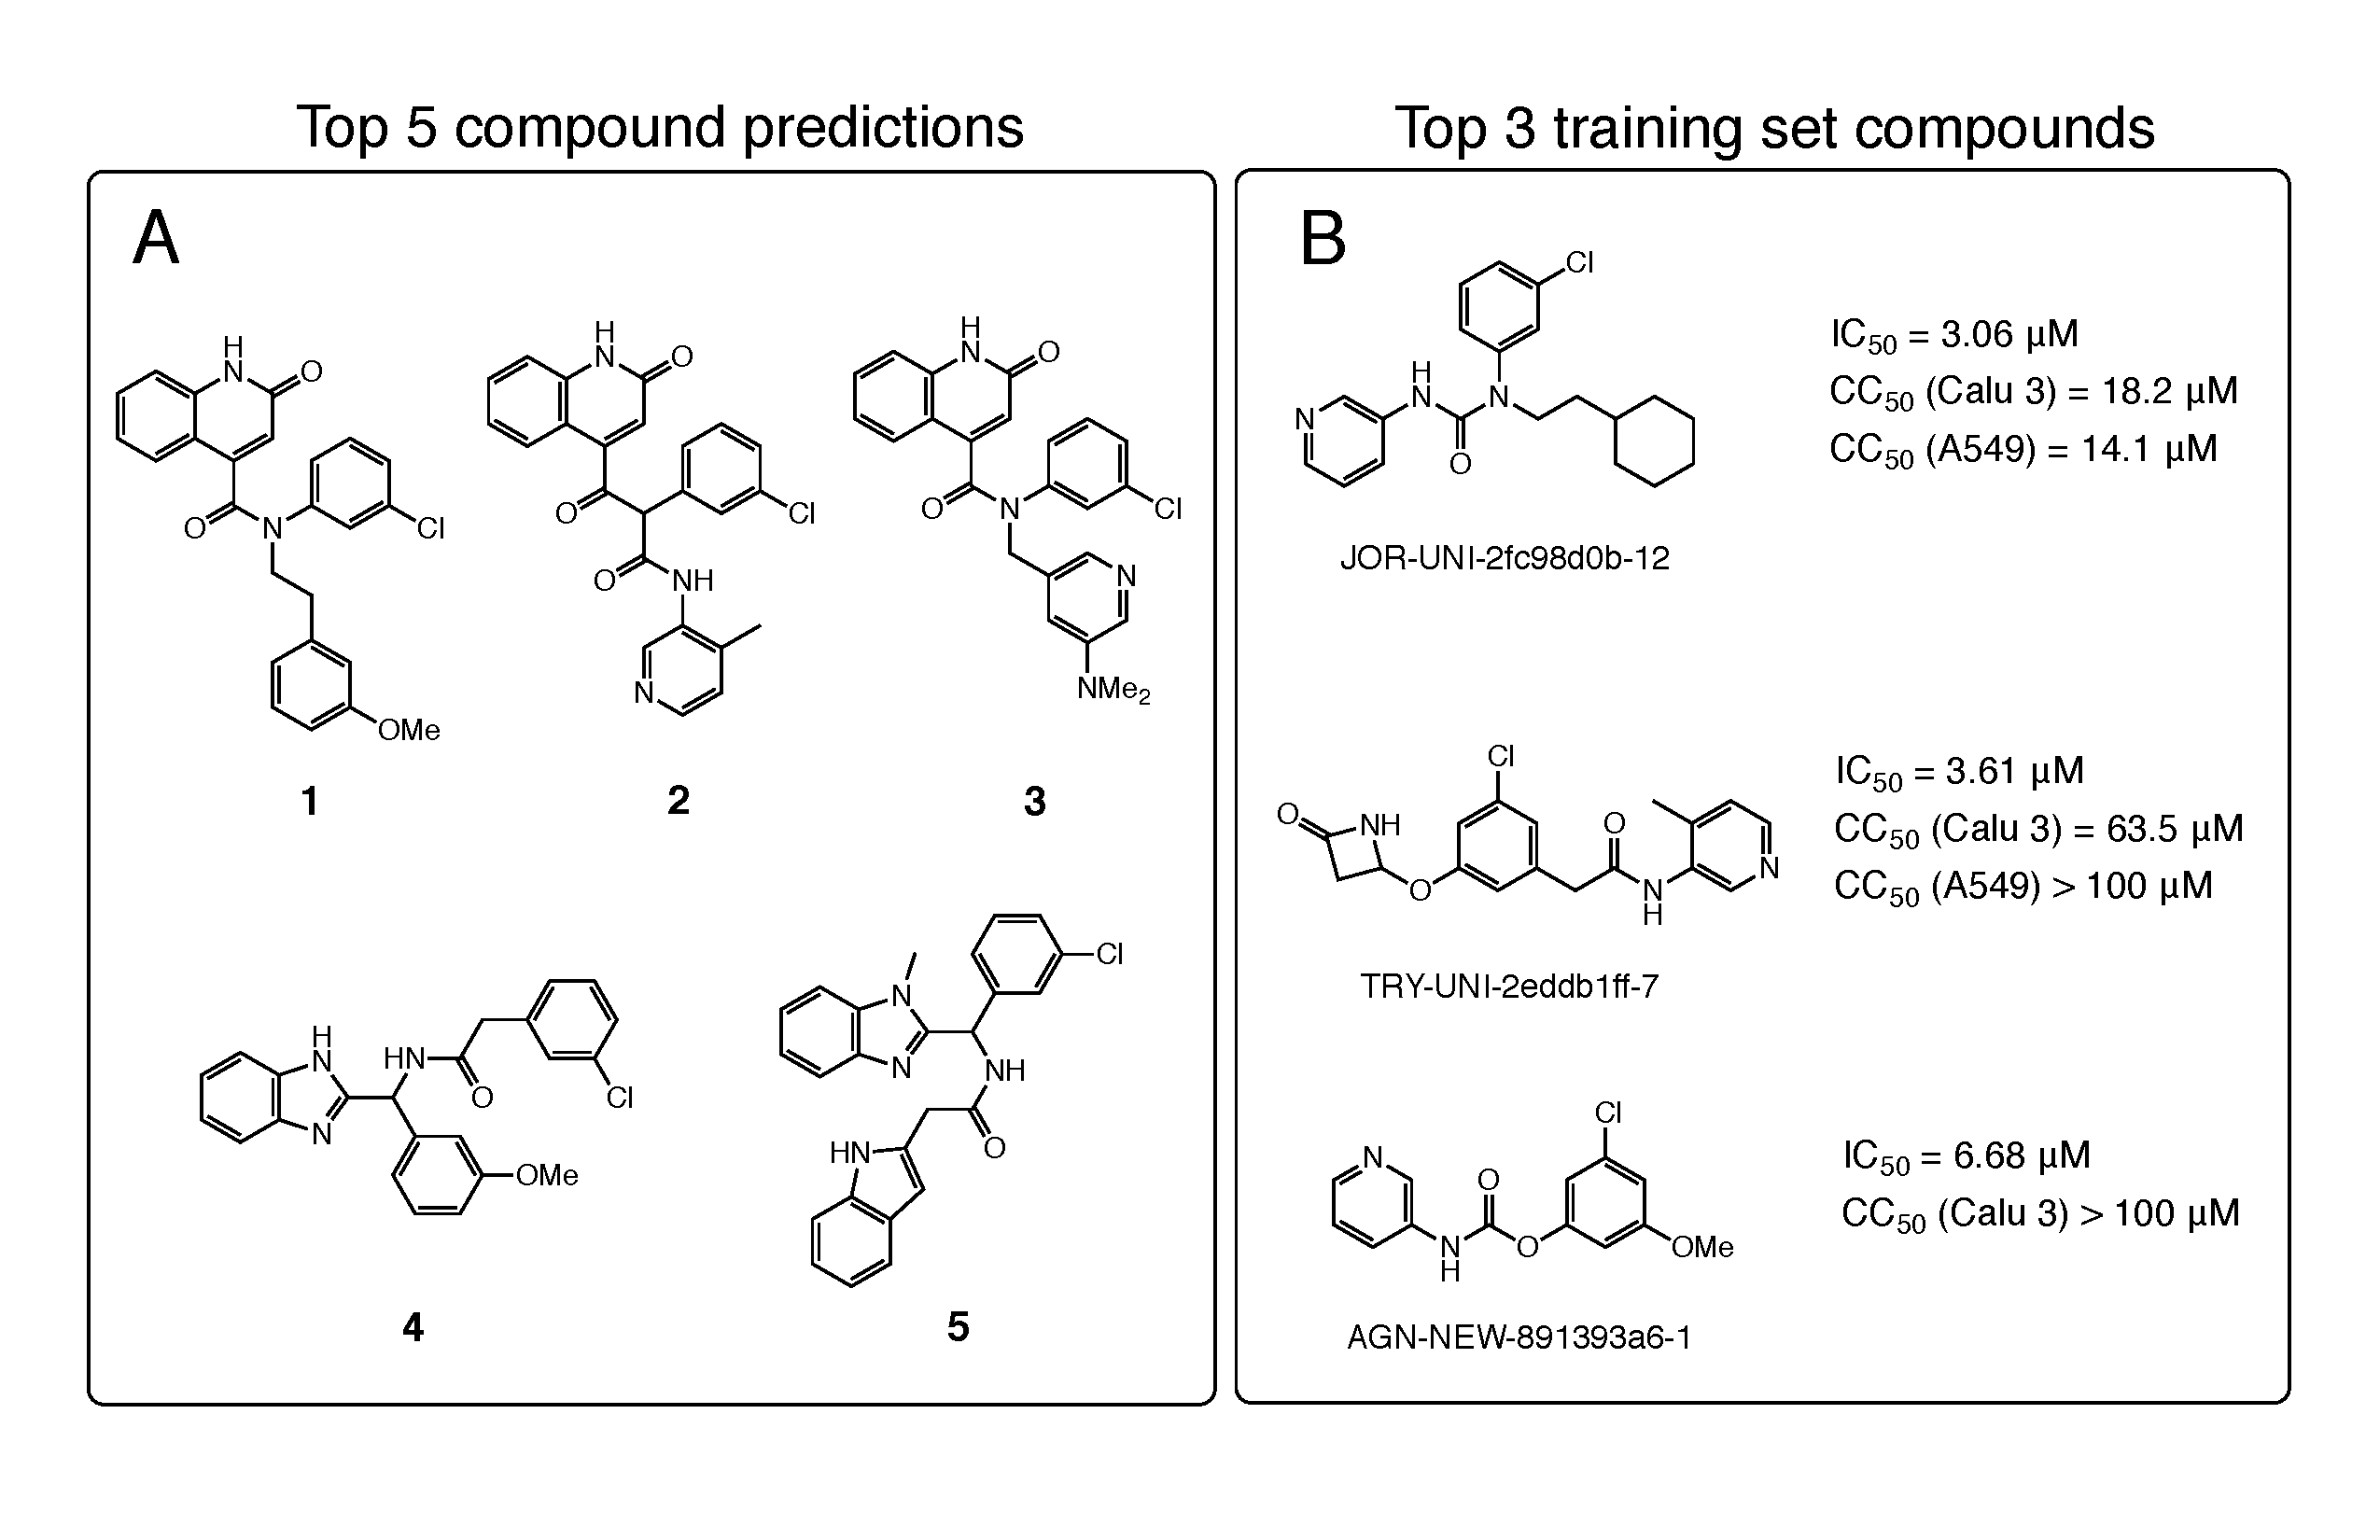
\includegraphics[width=0.75\textwidth]{Chapters/Ranking/Figs/fig2.pdf}
 \caption{\textbf{Our synthesis-driven design model prioritises molecular scaffolds that are not in the top hits.} (A) The 5 compounds selected by our methodology for synthesis and testing. (B) The top 3 compounds from the training set, with potency and cytotoxicity measurements.}
 \label{fig:compounds}
\end{figure}

Although virtual ``reactions'' were used to generate new molecules, the synthons are not necessarily off-the-shelf nor the reactions optimal. As such, we use a retrosynthesis predictor to triage based on synthetic accessibility. We used Manifold, a platform for synthesis route prediction (\url{https://postera.ai/manifold}), to generate synthetic routes for the model's top-ranked molecules starting from purchasable building blocks. The underlying technology is based on Molecular Transformer, a machine learning model for reaction prediction using sequence-to-sequence translation \citep{yang2019molecular,schwaller2019molecular}. The top 5 molecules from the screening library with <4 steps in their predicted routes were synthesised and tested (Figure \ref{fig:compounds}A). For comparison, the most potent molecules from the training set are shown in Figure \ref{fig:compounds}B. All five compounds have Tanimoto similarity <0.48 (1024-bit ECFP6) to any molecule in the training set, indicating that the model is not merely reproducing molecules similar to the most potent actives but is exploring novel scaffolds.

\begin{figure}[!th]
 \centering
 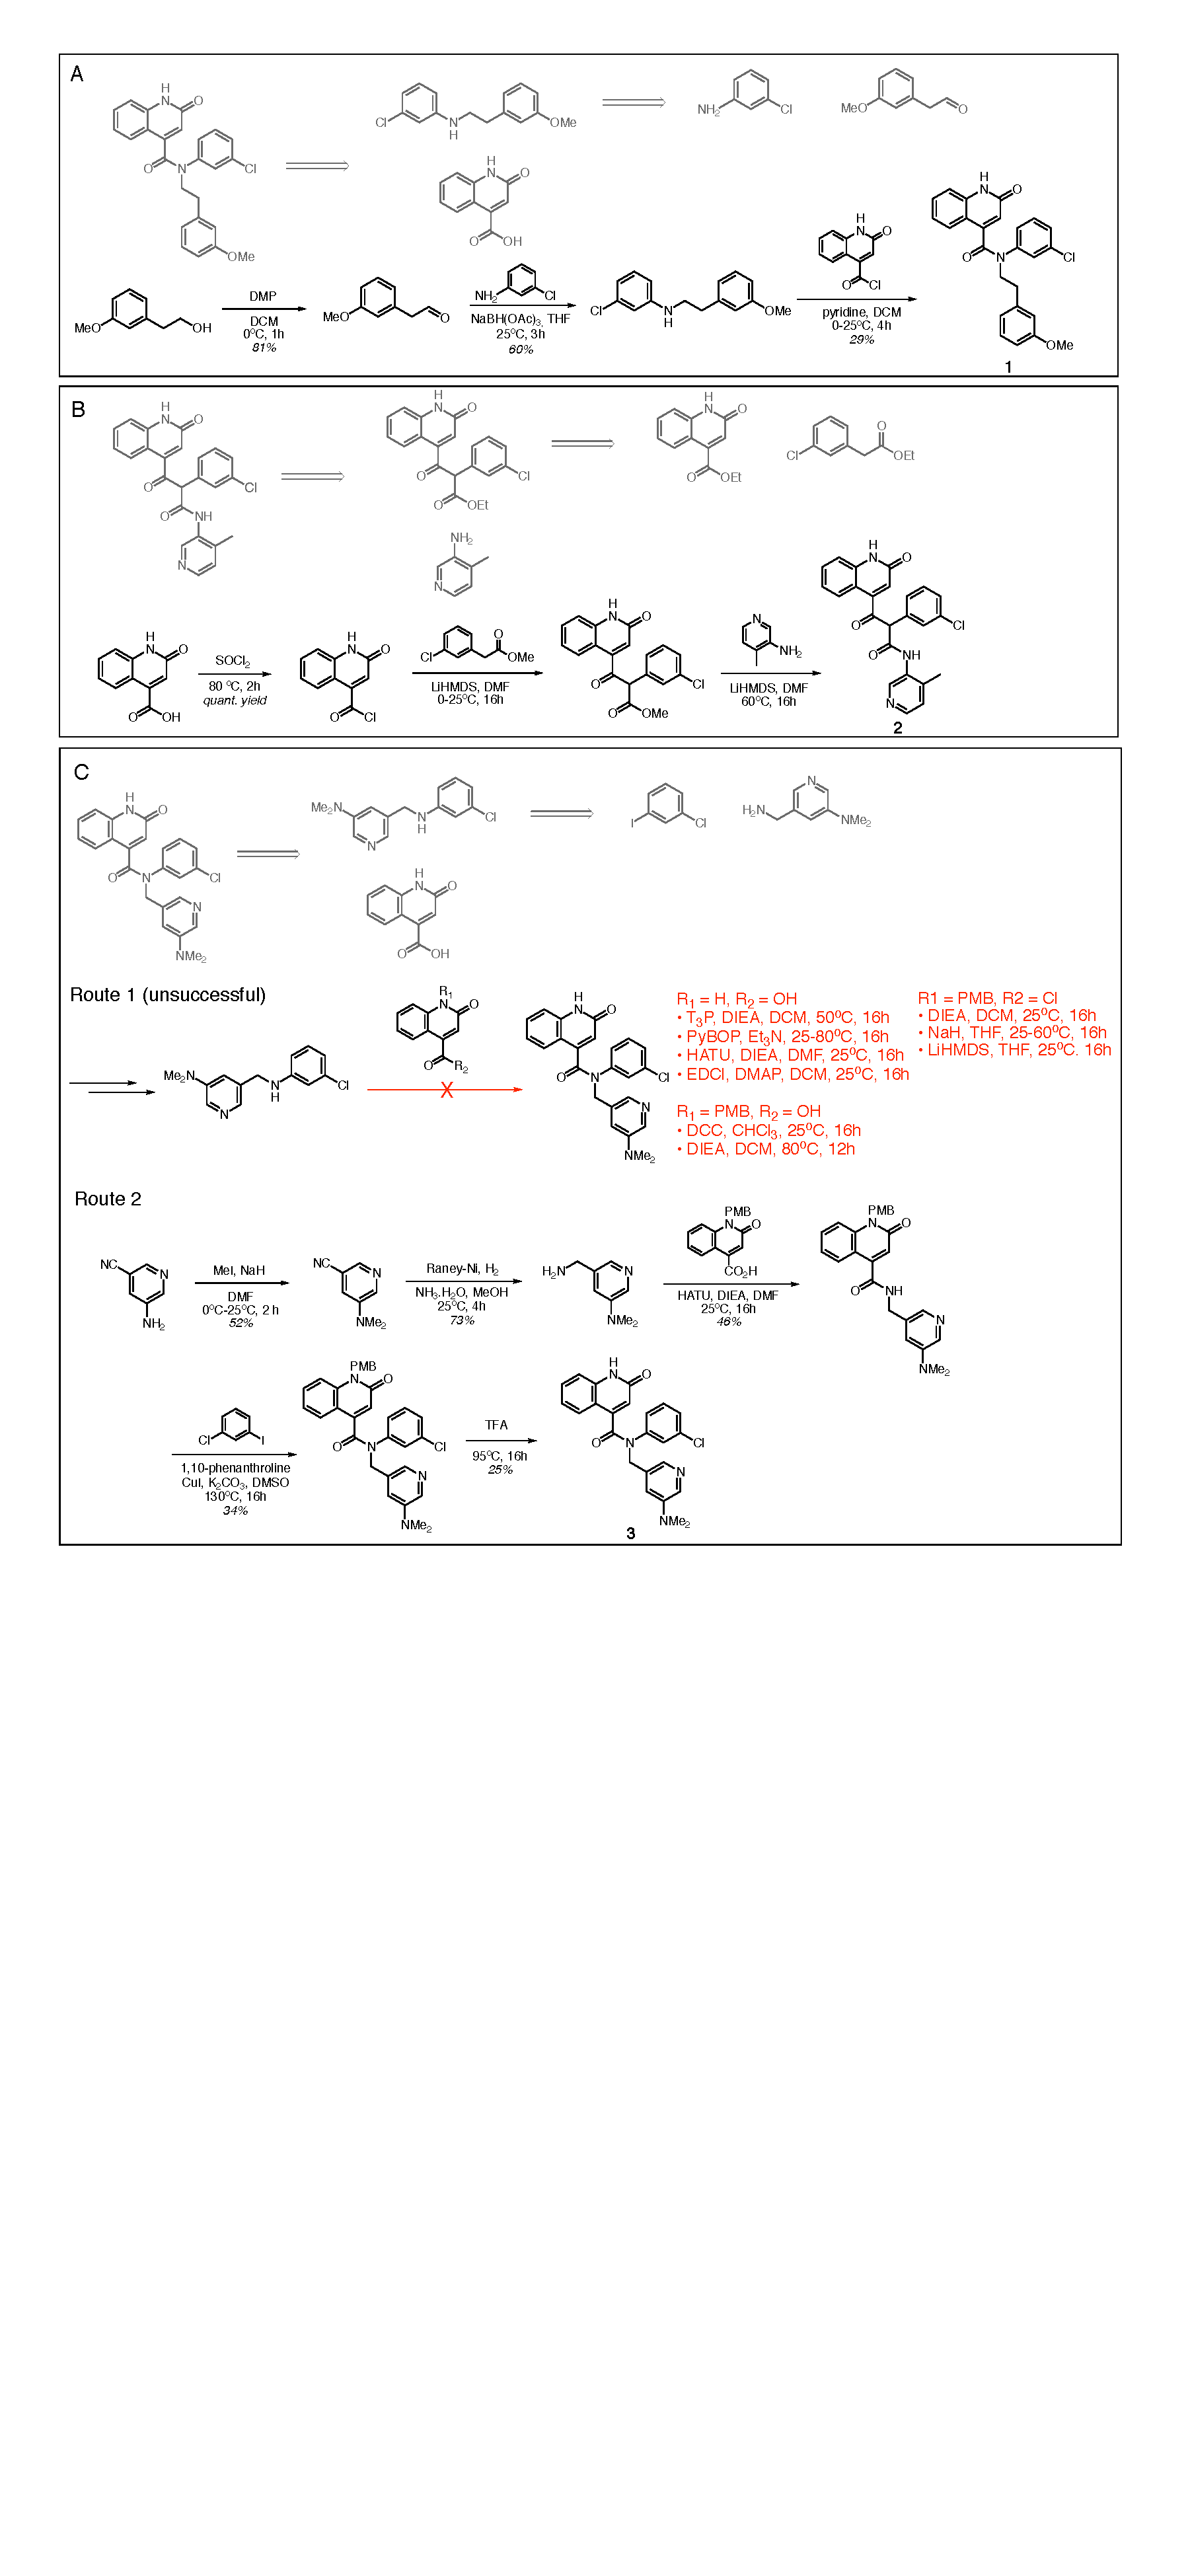
\includegraphics[width=0.65\textwidth]{Chapters/Ranking/Figs/rxn_schemes_1_to_3.pdf}
 \caption{\textbf{Model generated synthetic schemes that are experimentally validated.} Schemes (A)-(C) show the synthesis schemes generated by our model (grey) and experimental schemes (black) for Compounds $\mathbf{1}$-$\mathbf{3}$. The schemes for compounds $\mathbf{4}$ and $\mathbf{5}$ can be found in Appendix \ref{appendix:rxn_schemes}.}
 \label{fig:synthesis_schemes}
 \end{figure}

Figure \ref{fig:synthesis_schemes} shows that for Compounds $\mathbf{1}$, $\mathbf{2}$, $\mathbf{4}$ and $\mathbf{5}$ our retrosynthesis algorithm generates successful routes, thus provides a reasonable estimate of synthetic complexity. The syntheses were carried out at the Wuxi AppTec and compounds were assayed as received. Minor variations in building blocks were employed depending on what was readily available. We note that our algorithm failed to estimate the synthetic complexity of Compound $\mathbf{3}$. The final amide formation step was unexpectedly challenging, and no desired product was seen despite significant efforts in condition screening. Compound $\mathbf{3}$ was furnished via an alternative strategy, employing an Ullmann coupling to arylate the amide, which was not predicted by our approach. 

\begin{figure}[!th]
 \centering
 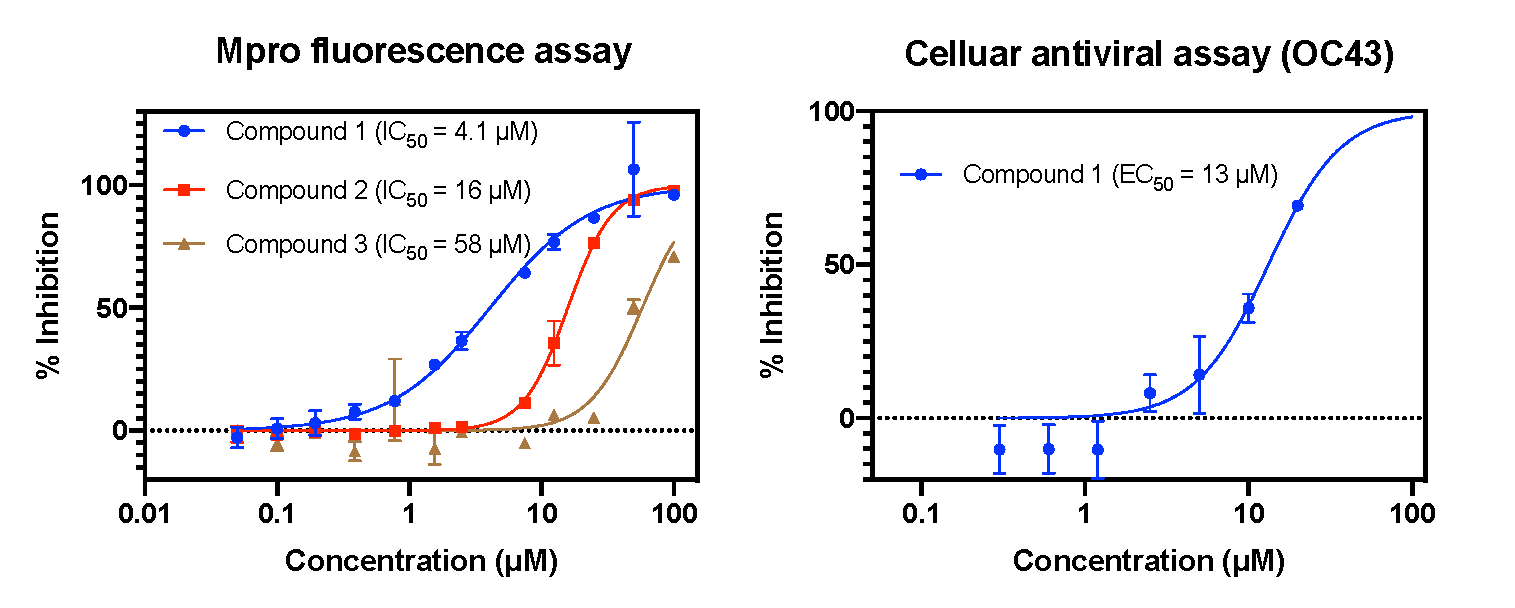
\includegraphics[width=0.85\textwidth]{Chapters/Ranking/Figs/data_curve.pdf}
 \caption{\textbf{Three compounds generated using our synthesis-directed model exhibit Mpro activity.} Our most active compound has measurable antiviral activity against the OC43 coronavirus and no measurable cytotoxic effect.}
 \label{fig:data}
\end{figure}

%result + discussion 
Compounds $\mathbf{1}$-$\mathbf{5}$ were tested for Mpro activity using a fluorescence assay. Figure \ref{fig:data} shows that Compounds $\mathbf{1}$-$\mathbf{3}$ have $\mathrm{IC}_{50}$ within assay dynamic range ($<100 \mu$M), and Compound $\mathbf{1}$ has $\mathrm{IC}_{50} = 4.1 \mu$M (95\% CI: [3.42,4.86]). Compound $\mathbf{1}$ is further assayed in live virus assays, with the less pathogenic OC43 coronavirus, showing $\mathrm{EC}_{50} = 13 \mu$M (95\% CI: [10.1, 18.4]) and is not cytotoxic ($\mathrm{CC}_{50}>100 \mu$M against A549 cell line; $CC_{50}$ is the concentration required to cause 50\% cell death). We employ OC43 as a rapid surrogate assay for SARS-CoV-2 as the former can be done in a BSL-2 rather than BSL-3 lab (See Appendix \ref{appendix:experiments} for assay details). %Interestingly, the top non-cytotoxic hit of the training set (TRY-UNI-2eddb1ff-7) does not show OC43 activity, showcasing the utility of using generative models to suggest new scaffolds with complementary physicochemical properties. 

\section{Discussion} \label{sec:discussion}

In summary, we demonstrated the utility of a \emph{de novo} design framework that learns to rank bioactivity and estimates synthetic complexity, for generating ideas in hit expansion. At the time of writing, optimisation of a quinolone-based scaffold is ongoing in the COVID Moonshot initiative (\url{https://postera.ai/covid}). Data for Compound $\mathbf{1}$-$\mathbf{5}$ is registered as the $\texttt{ALP-POS-ddb41b15}$ series on the Moonshot platform. 

The learning-to-rank approach presented in this chapter is a promising technique for maximally utilising data from inactive compounds as well as accounting for noise in the experimental values. Further work extending this approach to utilise information from ligand-protein complexes has shown great success in hit-to-lead optimisation \cite{Saar2023pnas}. By using docking-based structural descriptors as the input to their ranking model, the authors were able to utilise crystal structures of inactive compounds and outperform docking as well as a fingerprint-based ranking model on ranking ligand activity. Applying this model to docked structures from a virtual library, the authors were able to greatly improve the potency from their starting point and extended the ligand into unknown regions of the binding site. This result shows the potential for applying ranking-based approaches for modelling bioactivity.

A caveat for pair-based ranking is that even for moderately sized datasets the number of molecular pairs (which is proportional to the square of the dataset size) may become very large and therefore unfeasible to train on. Engineering approaches for efficient sampling of molecular pairs, such as using Tanimoto similarity to constrain pair selection, may be necessary and should be the subject of future work.

% discuss the potential of estimation synthetic complexity for drug design workflows and incorporating it for automated design
The AI-based estimation of synthetic feasibility played a critical role in compound selection in this work and is a promising enabler for automated design workflows in drug discovery \cite{Goldman2022ChemicalDesignLevels}. Beyond the capability to triage libraries by synthesizability and to guide the design of synthetic routes, ML synthesis models could play a key part in an automated drug design workflow. Utilising an automated workflow for the automatic generation of molecular designs as well as decision-making could potentially reduce iteration cycle time, require fewer compounds and iterations to produce a candidate, and scale to more programs \cite{Schneider2018AutomatingDrugDiscovery, Coley2020Outlook}. The framework presented in this chapter is an example of an automated design workflow albeit only with a single iteration - utilisation of multiple iterations via an optimisation \cite{korovina2019chembo} or reinforcement learning feedback loop \cite{born2019paccmannrl} will be a challenging but exciting area of future work.

% \begin{table}[!h]
% \caption{Graph SNN pairwise ranking results}
% \centering
% \label{table:pairwise_table}
% \begin{tabular}{l c c}
% \toprule
% Series & ROC-AUC & PRC-AUC \\ 
% \midrule
% Chloroacetamides & 0.80 & 0.71 \\

% Acrylamides & 0.78 & 0.80 \\

% Non-covalents & 0.74 & 0.74 \\
% \bottomrule
% \end{tabular}
% \end{table}

% The performance metrics indicate that the model is able to reliably classify whether one compound is more active than another, in particular with much better precision-recall than seen in simply classifying activity.
\chapter{Quantitative Interpretation of Reaction Prediction Models}\label{ch:transformer}

\begin{quote}
    This chapter is based on Dávid Péter Kovács, William McCorkindale and Alpha A. Lee. Quantitative interpretation explains machine learning models for chemical reaction prediction and uncovers bias. \textit{Nature Communications} volume 12, Article number: 1695 (2021)
\end{quote}

\noindent\hfil\rule{0.5\textwidth}{.4pt}\hfil

Organic synthesis remains a a major challenge in drug discovery. Although a plethora of machine learning models have been proposed as solutions in the literature, they suffer from being opaque black-boxes. It is neither clear if the models are making correct predictions because they inferred the salient chemistry, nor is it clear which training data they are relying on to reach a prediction. This opaqueness hinders both model developers and users. In this chapter, we quantitatively interpret the Molecular Transformer, the state-of-the-art model for reaction prediction. We develop a framework to attribute predicted reaction outcomes both to specific parts of reactants, and to reactions in the training set. Furthermore, we demonstrate how to retrieve evidence for predicted reaction outcomes, and understand counter-intuitive predictions by scrutinising the data. Additionally, we identify Clever Hans predictions where the correct prediction is reached for the wrong reason due to dataset bias. We present a new debiased dataset that provides a more realistic assessment of model performance, which we propose as the new standard benchmark for comparing reaction prediction models.

\section{\label{sec:intro}Introduction}

Organic synthesis remains a challenge in small molecule drug design, sinking time in the design-make-test cycle and potentially limiting the complexity of chemical space being explored \cite{blakemore2018organic,bostrom2018expanding}. The challenge of synthesis planning lies in searching through myriad of possible reactions to find optimal routes, and in predicting whether each possible reaction is indeed feasible and high yielding for the particular substrate in question. The problem of efficient search in synthesis has been recently addressed, inspired by innovations in computer science on searching and gameplay \cite{segler2017neural,segler2018planning,kishimoto2019depth,schreck2019learning, segler2019world}. However, accurately predicting the outcome of chemical reactions remains a hurdle \cite{Coley2018, Johansson2020, Struble2020}.

The current state-of-the-art in reaction prediction is the Molecular Transformer \cite{Schwaller2019}, which employs the transformer neural network architecture that was first introduced for neural machine translation \cite{Vaswani2017}. The input to the model is a text representation of the chemical structures of the reactant and reagent, and the model performs machine translation to predict most likely output molecule with a probability score. The Molecular Transformer achieves a 90\% Top-1 accuracy on the USPTO dataset of organic reactions that was text mined from US patents \cite{Lowe2012} and filtered \cite{Jin2017}. Recent work shows that thorough dataset augmentation improves model performance by allowing it to consider different equivalent SMILES representations \cite{tetko2020state}.

However, a key stumbling block in the Molecular Transformer is the lack of interpretability. Why the Molecular Transformer predicts one reaction outcome over another, and which training set reactions it finds most similar when reaching a particular prediction, are both unclear. Quantitative interpretability is crucial to both model users and model developers.

For model users, interpretability is important because chemical reactions are highly contextual, with important anthropomorphic metadata that the model overlooks. For example, reactants, reagents and products are only a part of the reaction. The reaction conditions, the scale of a particular reaction (e.g. discovery chemistry or scale up), and scientific focus of the project (e.g. total synthesis, medicinal chemistry or methods development) are some of the context that a skilled chemist can employ to interpret and understand the reaction.

For model developers, physical organic chemistry principles explain chemical reactivity and selectivity. As such, probing whether rationales outputted by the Molecular Transformer are congruent with physics allows developers to interrogate whether the Molecular Transformer is getting the correct prediction for the right reasons, and design model improvements based on those insights. 

In this chapter, we develop a suite of methods that quantitatively interprets the Molecular Transformer by attributing predictions to the input chemical structure and the training data. We illustrate our two-prong approach via a series of examples, showing how we uncovered what the model is learning, what it finds difficult, and explains its failure modes. Our method discovers hidden biases in the training data that hinder generalization performance and masks model shortcomings, which we resolved by introducing a new unbiased train / test split. 

\section{Molecular Transformer}
The Molecular Transformer \cite{Schwaller2019MolecularPrediction} is a tailored version of the Transformer architecture \cite{Vaswani2017} which was designed for machine translation and has had wide-ranging success in many Natural Language Processing tasks. It has an encoder-decoder structure, where both the encoder and the decoder are made up of so called transformer blocks. These blocks process the inputs by applying a multi-head scaled dot-product attention mechanism followed by layer normalization and some fully connected feed forward layers. An in-depth review of the attention mechanism can be found in \cite{Niu2021AttnReview}.

In Transformer models for text, we first break down the string input to the model into individual tokens and generate a learnt vector embedding for each token. To include the relative order of the tokens and thus distinguish tokens of the same type at different positions, an additional vector is generated based on the token positions (known as the positional encoding) and added to the token embeddings. This sequence of token embeddings is then input into the encoder and decoder layers. The encoder layer is responsible for encoding the input sequence into an informative vector representation to input into the decoder layer. The decoder layer reads the output from the encoder  layer and generates the output sequence. During model training, we train the decoder layer to predict the next token in the sequence given the previous tokens in the sequence. During model inference, the predictions are generated in an autoregressive way meaning that the decoder predicts one token at a time and the previously generated tokens are fed into the decoder when generating the next tokens. The prediction is considered final when an \texttt{<end>} token is generated or a pre-specified maximum length is reached. Through this process each translation gets assigned a probability score:

\begin{equation}
    P(\textrm{tgt} \mid \textrm{src}) = \prod_{i=1}^N P(\textrm{tok}_i \mid \textrm{tok}_1, \cdots , \textrm{tok}_{i-1}, \textrm{src}) 
\end{equation}
where $\textrm{tok}_i$ is the $i$-th predicted token and $N$ is the length of the prediction.

\begin{figure}[ht!]
    \centering
    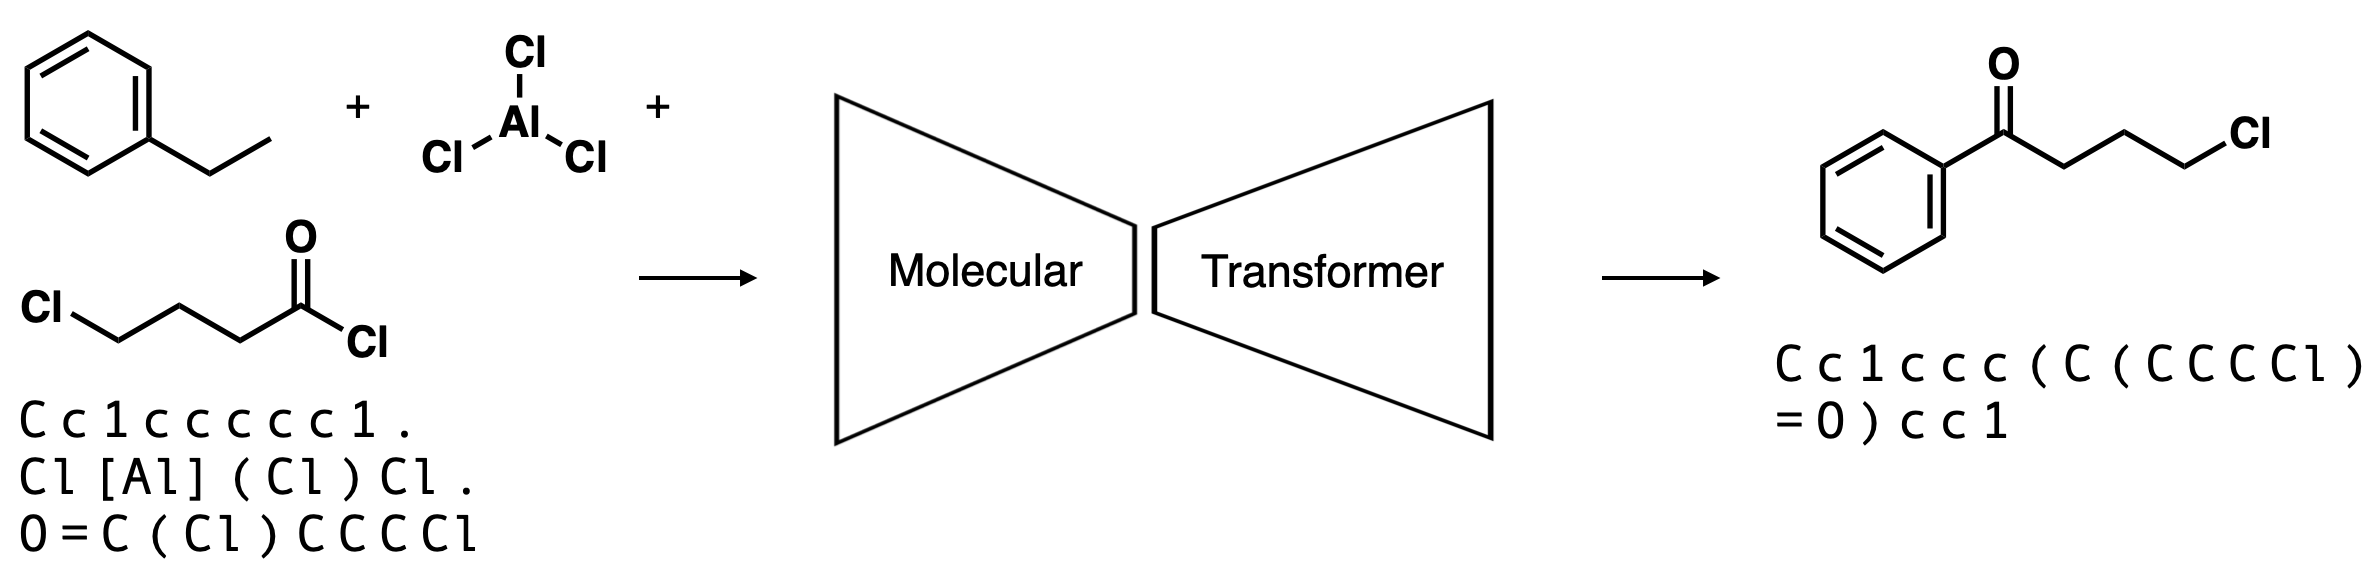
\includegraphics[width=0.8\textwidth]{Chapters/Transformer/Figs/mol_transformer.png}
    \caption{\label{fig:mol_transformer} \textbf{Schematic illustration of the Molecular Transformer.} The inputs to the model are tokenized SMILES of the reactants and reagents, and the model performs machine translation to predict the most likely product molecule with a probability score.}
\end{figure}

The Molecular Transformer (Fig~\ref{fig:mol_transformer}) uses this approach to perform reaction prediction by using tokenized SMILES of reaction reagents and reactants as input, and the tokenized SMILES of the reaction product as output. Typically, the SMILES of the reaction product are canonicalized while both canonical as well as non-canonical SMILES are used for the reactants and reagents as that has been shown to improve model performance \cite{Bjerrum2017SMILESaugmentation} compared to only using canonical SMILES. In addition, no distinction is made between "reactant" and "reagent" and the model is only trained on reactions with a single reaction product.

\subsection{Training data}
The training data used in this study was obtained by the text mining work of Lowe \cite{Lowe2012}, where organic reactions from US patents filed between 1976 and 2016 were extracted. The dataset was filtered by Jin et. al. \cite{Jin2017} to remove duplicates and some of the erroneous reactions which resulted in a set of ca 480 000 organic reactions. We found that this dataset, though much cleaner, still contained a large number of erroneous reactions whose sole product were halogen ions, nitric, sulphuric or phosphoric acids etc. We verified that the Molecular Transformer indeed learns these reactions if they are present in the training, resulting in catastrophic overfitting and unphysical predictions in some cases. To eliminate this effect we deleted a further ~8 000 reactions to obtain a dataset of 471 791 reactions. From this number we used 377 419 for training, 23 589 for validation and 70 765 as a hold-out test set. The training set was augmented by an equal number of random equivalent SMILES strings following the protocol of Schwaller et. al. \cite{Schwaller2019}. We trained a Molecular Transformer model as described in the original paper and were able to achieve 88.8\% Top-1 accuracy on the test set, similarly to the original paper. This model was used throughout the interpretability experiments.

An important aspect of the training data is that since it was extracted from patented reactions, it naturally contains a number of biases. Firstly there are no negative results included meaning that any combination of reactants and reagents in the dataset leads to a well defined product. This is in contrast to reality where often there is no reaction, or the product is a mixture of many different compounds. This bias will always be reflected in the machine learning models predictions. A further bias stems from the distribution of reaction types in the dataset. Most of the patented reactions come from the medicinal chemistry community leading to reactions popular amongst medicinal chemists being over-represented. This bias can be useful since the model learns the kind of reactions medicinal chemists like using \cite{Bjerrun2020} but it also hinders generalization because popular reactions are not necessarily better as has recently been shown in the case of inorganic chemical reactions \cite{Jia2019}.

\section{Quantitative Interpretation methods}

\begin{figure}[ht!]
    \centering
    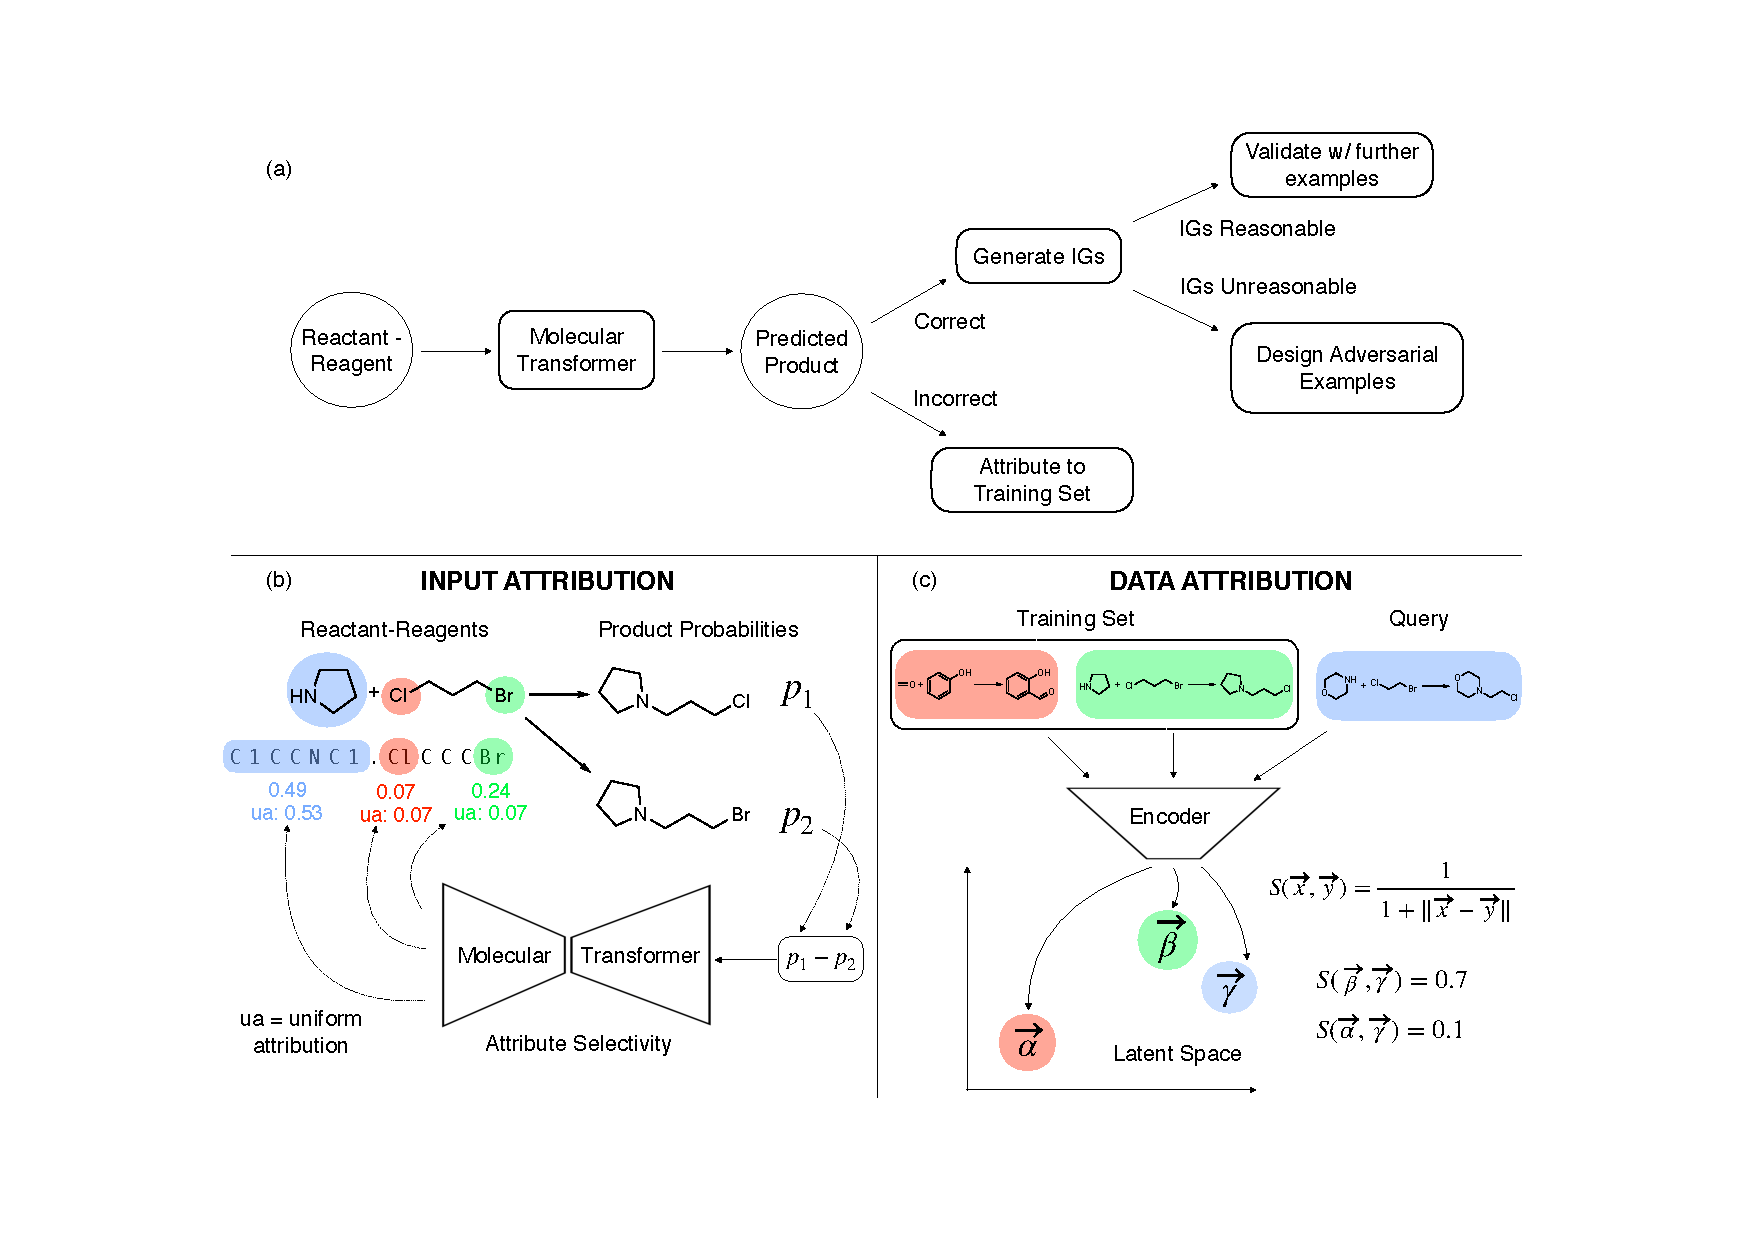
\includegraphics[width=0.8\textwidth]{Chapters/Transformer/Figs/workflow.pdf}
    \caption{\label{fig:workflow} \textbf{Schematic illustration of the attribution workflow.} (\textbf{a}) Overview of our workflow to interpret the Molecular Transformer. (\textbf{b}) Schematic of how the predicted probability difference between two products are attributed back to the reactant-reagent string in order to interpret the model's understanding of selectivity. The IG attributions below the reactant SMILES are compared to the uniformly distributed probability difference (ua) below. (\textbf{c}) Schematic of how the latent space encoding of reactant-reagent strings are used to infer the learnt similarity between query reactants and those from the training set.}
\end{figure}

There are three key factors determining the prediction of a machine learning model: the architecture, the training data and the input. Neural network models are often considered as black-boxes because of the complex ways these three factors interact to yield a prediction. 

To interpret model prediction, we first need to define what interpretability means. We suggest interpretability is the ability to discover associations and counterfactuals between input and output, and the ability to query evidence in the data supporting a certain outcome. Our approach follows the accepted scientific process: A scientific theory usually identifies factors that are related to a certain outcome and conversely how the absence of those factors is related to absence of outcome. Furthermore the investigator needs to show pieces of evidence that support the theory.

We employ Integrated Gradients~\cite{Sundararajan2017} as a rigorous method for attributing the predicted probability difference of two plausible products of a selective chemical reaction to parts of the input. The attributions show how much each substructure is contributing to the predicted selectivity of the model. This is illustrated on Figure~\ref{fig:workflow}b. The values of the attributions are compared to the value each subgroup would receive if the probability difference would be distributed evenly across the input. The parts of the structures getting higher IGs than the uniform attribution (ua) are considered important. Details of the methods can be found in Section~\ref{subsec:input_attribution}. 

Attributing the predictions of neural networks to most similar training data points is less widely researched. To achieve this goal we developed a new method based on the latent space similarity of the reactions. We used the outputs of the Molecular Transformer encoder averaged over the tokens to achieve a fixed length vector representation of the reactions. The most similar training reactions according the model were than identified using the Euclidean distance of these latent space vectors. A schematic overview of our method is shown on Figure~\ref{fig:workflow}c. Details of the methods can be found in Section~\ref{subsec:data_attribution}.

We validate our interpretations in two ways. The first is via falsification. If the integrated gradients attributions are chemically unreasonable, i.e. predictions are correct for the wrong reasons, we design adversarial examples that force the model into wrong predictions. The second is by identifying causes for the prediction in the training data. If a prediction is wrong, we interrogate whether a similarly incorrect entry is in the training data. 

\subsection{Input attribution} \label{subsec:input_attribution}
To unpack the Molecular Transformer we decided to focus our efforts on reactions containing selective chemical transformations which means that they have multiple plausible outcomes. These reactions are most fit for identifying if the model is making the predictions on true chemical basis because the underlying chemical causes are well established. Our general framework of interpreting chemical reactions is shown on Figure~\ref{fig:workflow}a.

Once a suitable chemical reaction with two possible target molecules is chosen the Molecular Transformer probability scores of the products are generated. The difference in probability score between the true and the incorrect but plausible products is than attributed back to the reactant reagent inputs.

Recently there were many methods developed and applied successfully for attributing the predictions of neural networks to parts of the input. Some of the most notable examples are LIME, SHAP, Layer-wise Relevance Propagation (LRP) and Integrated Gradients \cite{Ribeiro2016WhyClassifier, Lundberg2017APredictions, Montavon2018MethodsNetworks, Sundararajan2017}. These methods are designed to propagate back the output of the models in a fair way to determine the contribution (importance) of each of the input features to the prediction. There are several methods that have their roots in cooperative game theory and are proven to yield fair attributions as defined by the axioms of fairness \cite{Sundararajan2017}. For machine learning models where the gradients are not readily available, there are so called Shapley-values and the closely related SHAP method \cite{Lundberg2017APredictions}. For models such as the Transformer where the gradients are easy to evaluate the Integrated Gradients (IGs) method is a more natural choice \cite{Sundararajan2017} though other methods such as LRP have also been applied successfully \cite{Karpov2020}. The IGs method has also been applied previously for interpreting language models in natural language processing applications and for designing adversarial examples in the context of question answering \cite{mudrakarta2018did}. A graphical illustration of IGs is shown on Figure~\ref{fig:workflow}b. Our approach builds on the work of McCloskey et.\,al.\,\cite{McCloskey2019} who used IGs to understand binding prediction by graph neural networks on artificial datasets. We extend the method to Transformer architectures, and use it in the context of reaction predictions on real experimental data.

IGs are calculated by evaluating the path integral of the gradient of the output with respect to the input along a straight line path in the input space from a non-informative baseline to the input of interest.

Given a neural network denoted by the function $F:\mathbb{R}^n\to [0,1]$, the input $x\in\mathbb{R}^n$ and the baseline input $x'\in\mathbb{R}^n$ the IG attribution of feature $i$ is given by

\begin{equation}
\label{eqn:IG}
    \textrm{IG}_i(x) = (x_i - x_i') \int_{\alpha=0}^1 \frac{\partial F(x' + \alpha(x-x'))}{\partial x_i} d\alpha
\end{equation}

In the case of the Molecular Transformer $x$ is the $ N\times 256$ dimensional embedding of the input SMILES string of length $N$ and $x'$ is the embedding of the \texttt{'.'} token taken $N$ times. This token is used in the SMILES language to separate different molecules and hence on its own bears no chemical information making it an ideal baseline choice. To obtain the total contribution of each of the input tokens the attributions are summed along the 256 dimensional embedding vectors.

Finally to make the attributions easier to interpret we devised a few simple rules to map the token level attributions to chemically meaningful substructures. Reagents like sulphuric acid or meta-Chloroperoxybenzoic acid (mCPBA) are fed into the model by their full SMILES strings but in reality they act as single units as far as the reaction is concerned. Their attributions are more meaningful to look at as a whole rather than token by token. A related problem is with the attributions corresponding to special characters in SMILES like numbers or parentheses. To resolve this we consider rings as single units and their attribution is calculated by summing over the ring atoms and numbers. This way the information about the relative positions of the ring substituents will also be included in the attribution of this part of the structure. Branches are also considered as single units and their attribution is the sum over their atoms and the parentheses specifying them.

For the attributions to be meaningful it is important to look at reactions where there are two possible products which have non-zero probability scores according to the model. This is crucial since for the prediction of a single product every token of the reactant is important, since missing a remote carbon would also result in a wrong prediction. By looking at the probability difference of two plausible products this effect can be eliminated and the attributions highlight the groups driving the chemical selectivity (according to the model). In particular, canonical SMILES for both products should be used to ensure the probability scores are non-negligible.

Finally, to determine if a particular group is important according to the model we compare its attribution to the attribution that would fall onto it, if the probability difference was distributed evenly across the input tokens. Substructures that get substantially higher attribution than uniform are most important for the model when it favours one product over the other.

\subsection{Training data attribution} \label{subsec:data_attribution}
Attributing the predictions of neural networks to training data can serve as a tool for explaining predictions as well as gaining understanding of the models inner workings \cite{tetko2002}. In cases when a model predicts something very unexpected to humans attributions to parts of the input can be difficult to make sense of. Sometimes it can be much more illustrative to see a couple of example inputs that the model finds similar. Usually seeing a number of similar examples can help humans identify patterns that may serve as the basis of the model's prediction. This can either result in the discovery of new trends or laws in the scientific domain or it can reveal biases that the model has learnt. In the latter case this information can be used to improve the model or the dataset.

To create a successful method for attribution to data the most crucial element is the careful design of a similarity measure. The similarity should be defined such that it measures how similar two input datapoints are according to the model. For different neural network architectures different choices of similarity measures can be appropriate. In the case of feed-forward or convolutional architectures a natural choice is to define a fingerprint vector for each data point that consists of the neural networks layer outputs (activations) concatenated together. This similarity measure has been shown to be useful for judging the reliability of toxicity models predictions by comparing molecules not in the training set \cite{Allen2020}.

In the case of the Molecular Transformer which has an encoder-decoder architecture the output of the encoder layers can be used as a basis for comparing data points. Since the encoder hidden states have a non-fixed length we take the average of them across the input tokens to obtain a fixed-length $256$ dimensional vector representation for each of the reactions. Averaging is expected to work because of the relatively large dimensionality of the latent space. The size of the vocabulary of the USPTO dataset is 288 so there are almost as many orthogonal directions in the latent space as there are possible different input tokens. This is expected to lead to minimal loss of information upon averaging. For each reaction in the training set the 256 dimensional hidden state vector is generated and the matrix of training set reaction hidden states is saved as a binary. When a new example input is given to the model it is passed through the Transformer encoder and the average hidden state vector of it is calculated. A schematic diagram depicting the method is shown in (Figure~\ref{fig:workflow}b). The similarity score of the input reaction vector \textbf{u} to a training set vector \textbf{v} is calculated by

\begin{equation}
    \textrm{score}(\textbf{u},\textbf{v}) = \frac{1}{1 + \|\textbf{u} - \textbf{v} \|}
\end{equation}

In this work we inspect the top-5 most similar reactions from the training set for comparison with the input reaction.

\section{Investigation of Specific Reaction Classes}

We investigate in detail three reaction classes that are commonly used in medicinal chemistry. Through these examples we illustrate each of the three branches in Figure~\ref{fig:workflow}(a). We first examine the selective epoxidation of alkenes where the Molecular Transformer produces the right prediction for the right reason.

We then turn to the Diels-Alder reaction, which is a scaffold-building transformation widely used in synthesis. We show that the Molecular Transformer is not able to correctly predict this reaction. Following the bottom branch of Figure~\ref{fig:workflow}a we investigate it using Data attribution and find that the USPTO dataset contains very few instances of Diels-Alder reactions, likely explaining why the model is not able to predict the outcome correctly.

Finally we consider the Friedel-Crafts acylation reactions of substituted benzenes. We show that the Molecular Transformer predicts the right product for the wrong reason and validate our interpretation using a number of adversarial examples.

\subsection{Epoxidation}

\begin{figure}[ht!]
    \centering
    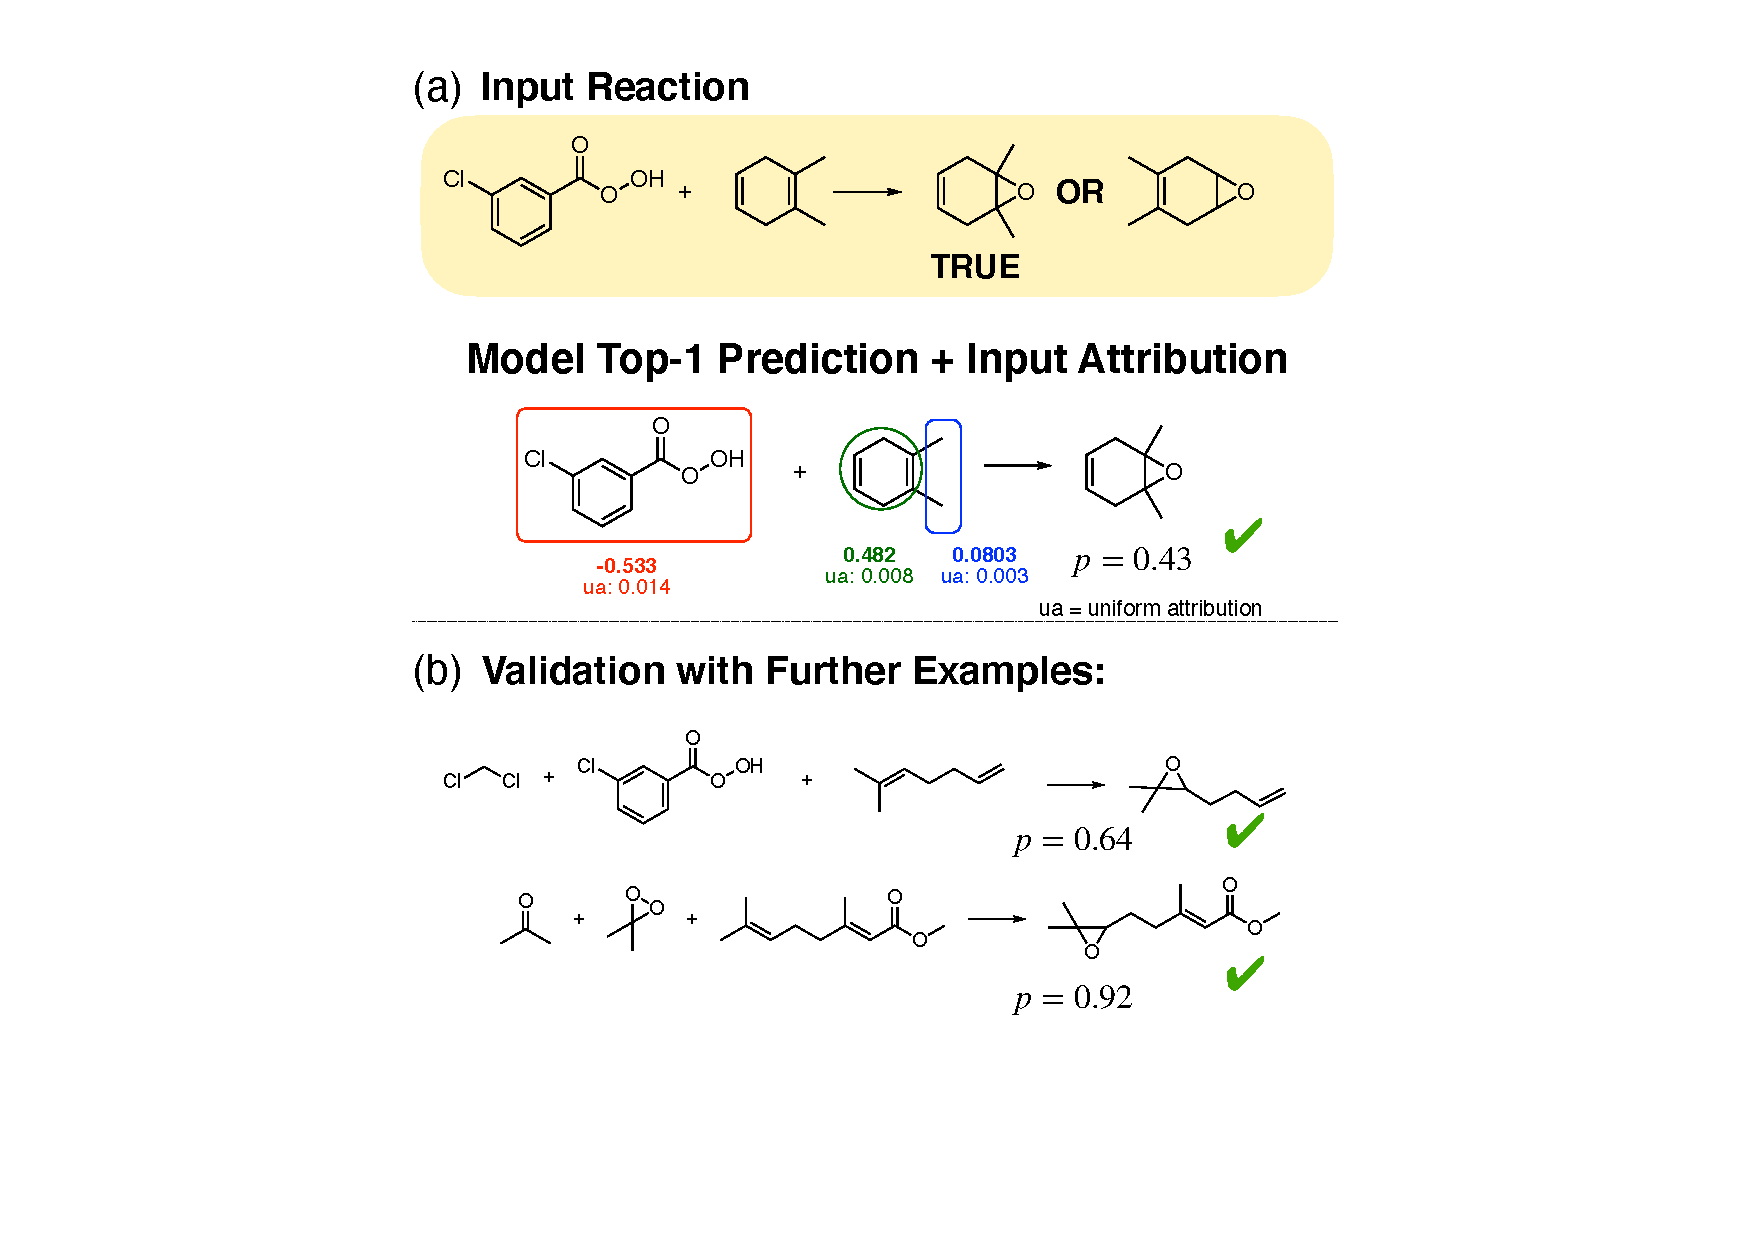
\includegraphics[width=0.6\textwidth]{Chapters/Transformer/Figs/epoxidation.pdf}
    \caption{\label{fig:epoxide} \textbf{IG attributions highlight correct model reasoning.} (\textbf{a}) The model correctly predicts the product of a typical epoxidation reaction, and shows significant positive attributions to the two methyl group that are responsible for the selectivity. (\textbf{b}) We validate the model's knowledge on two unseen epoxidation reactions from chemical literature~\cite{Lluch1993}}
\end{figure}

The oxidation of alkenes to form epoxides is an important intermediate reaction in many synthesis plans \cite{Clayden2012}. The common oxidant in these reactions are peroxy compounds. The most widely used example of them is mCPBA, which is a versatile reagent appearing 2052 times in the USPTO dataset. This is in the high data regime where we would expect the model to do well due to the large number of different training examples available. 

Epoxidation reactions can be regioselective, with more substituted alkenes reacting faster because they are more electron-rich \cite{Clayden2012}. A typical example reaction showing this type of selectivity is shown on Figure~\ref{fig:epoxide}a. 

The Molecular Transformer is able to predict the product with the correct selectivity, giving it a probability score of 0.43. The probability score of the alternative incorrect product was less only by 0.025. This is a case where the model predicts two similarly plausible outcomes, so IGs can help to judge whether or not a prediction can be trusted. Since the probability difference is close to 0, the sign of the attributions at different parts of the input is in itself interesting and contains information regarding the favoured outcome. 

Figure~\ref{fig:epoxide}a shows the IG attributions of the different parts of the input.  In this case the positive attributions favour the correct product while the negative attributions favour the incorrect product. The IGs show that the two methyl substituents circled with blue are significantly contributing to the correctly predicted selectivity. The attributions on the other parts of the molecule are harder to interpret. This can be the result of the model being uncertain in the prediction leading to larger gradients along the path integral during the calculation of the attributions. 

To validate the interpretation that the model has learnt this selectivity we generated the Molecular Transformer predictions for two further examples from the literature as shown on Figure~\ref{fig:epoxide}b. The first example is very similar to the one examined in detail above and the model is consistently predicting the correct product. The second example is more challenging for the model for a number of reasons. First the reagent is not mCPBA but dimethyldioxirane which appears much less frequently, only 14 times in the training data, secondly both double bonds are substituted, and the difference is made by a more subtle chemistry, the ester group being electron withdrawing. The model is able to predict the correct outcome here as well confirming that the predictions are correct for the right reason. 

\subsection{Diels-Alder}

\begin{figure}[ht!]
    \centering
    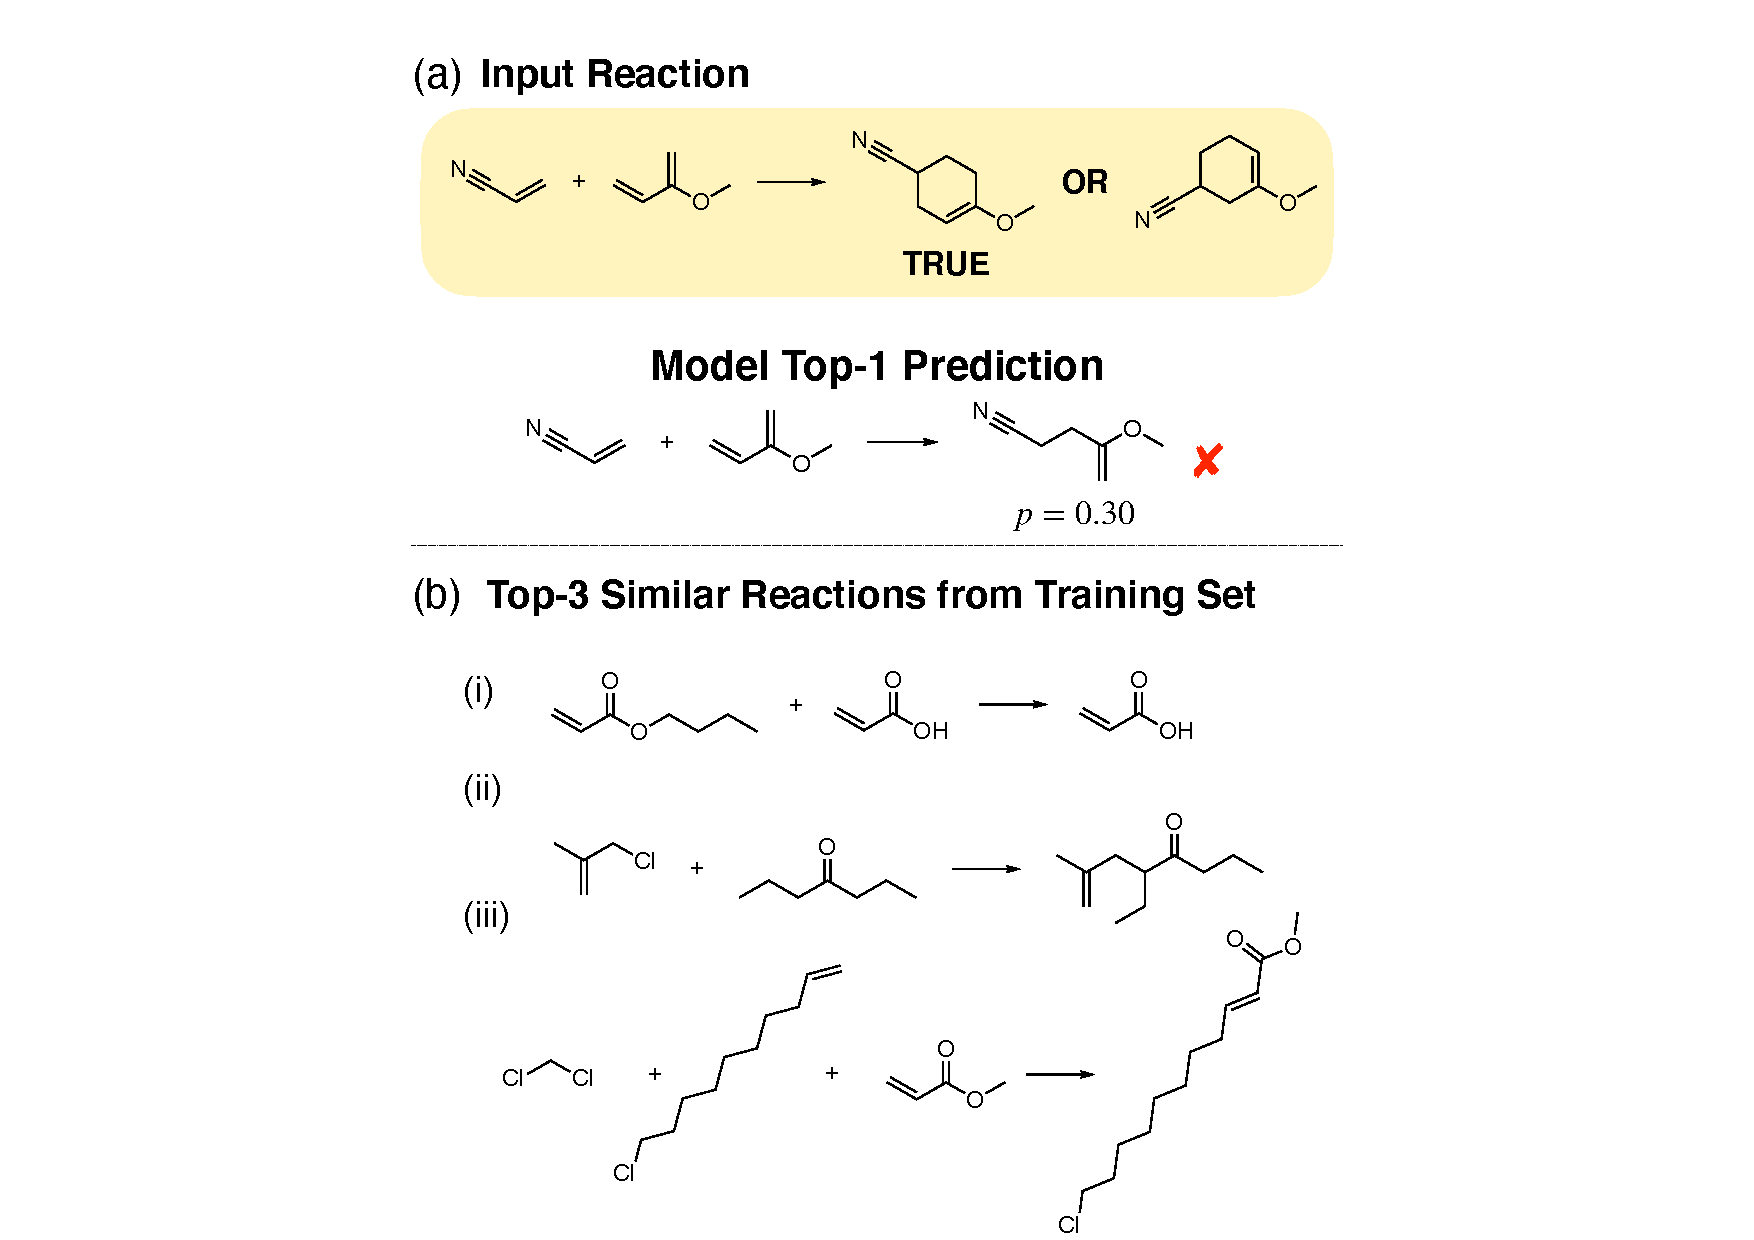
\includegraphics[width=0.6\textwidth]{Chapters/Transformer/Figs/diels_alder.pdf}
    \caption{\label{fig:diels_alder} \textbf{Data attribution explains erroneous predictions.} (\textbf{a}) The model makes an obviously incorrect prediction on a typical example of a Diels-Alder reaction with challenging selectivity. (\textbf{b}) Attribution to the USPTO training data shows that the model either completely fails to recognize Diels-Alder reactions or that no Diels-Alder reaction is present in the dataset.}
\end{figure}

The Diels-Alder reaction transforms a conjugated diene and an alkene (called dienophile) to a six membered ring with a double bond \cite{Clayden2012}. There are very few limitations on the character of the diene. It only has to be flexible enough to take up an s-cis conformation. The dienophile, on the other hand, should have carbon-carbon double bonds conjugated preferably with an electron withdrawing group. A typical example of a Diels-Alder reaction used as a test-case is shown on Figure~\ref{fig:diels_alder}a. 

The Molecular Transformer was unable to predict the regioselectivity of this reaction, and in fact the predicted product was clearly wrong with the actual possible products getting 0 probability scores. Since the prediction is obviously wrong, we followed the bottom branch of the workflow at Figure~\ref{fig:workflow}a and generated the most similar training reactions to see what causes this erroneous prediction.

Figure~\ref{fig:diels_alder}b shows the Top-3 most similar reactions from the training set based on the model encoder output similarities. The most similar training reaction (i) is an erroneous reaction, whilst the second and third are carbon-carbon bond formations, but via Grubbs methathesis \cite{grubbs} rather than cycloadditions. This means that the model has not learnt a good representation of Diels-Alder reactions in the latent space. 

To investigate if the cause of this was a lack of training data we devised a reaction template corresponding to the [4+2] cycloaddition and found that there were only 7 reactions matching it in the entire USPTO database. This example illustrates how attribution to data can be useful for identifying erroneous predictions caused partly due to erroneous data and partly due to the scarcity of training examples. 

\subsection{Friedel-Crafts Acylation}

\begin{figure}[ht!]
    \centering
    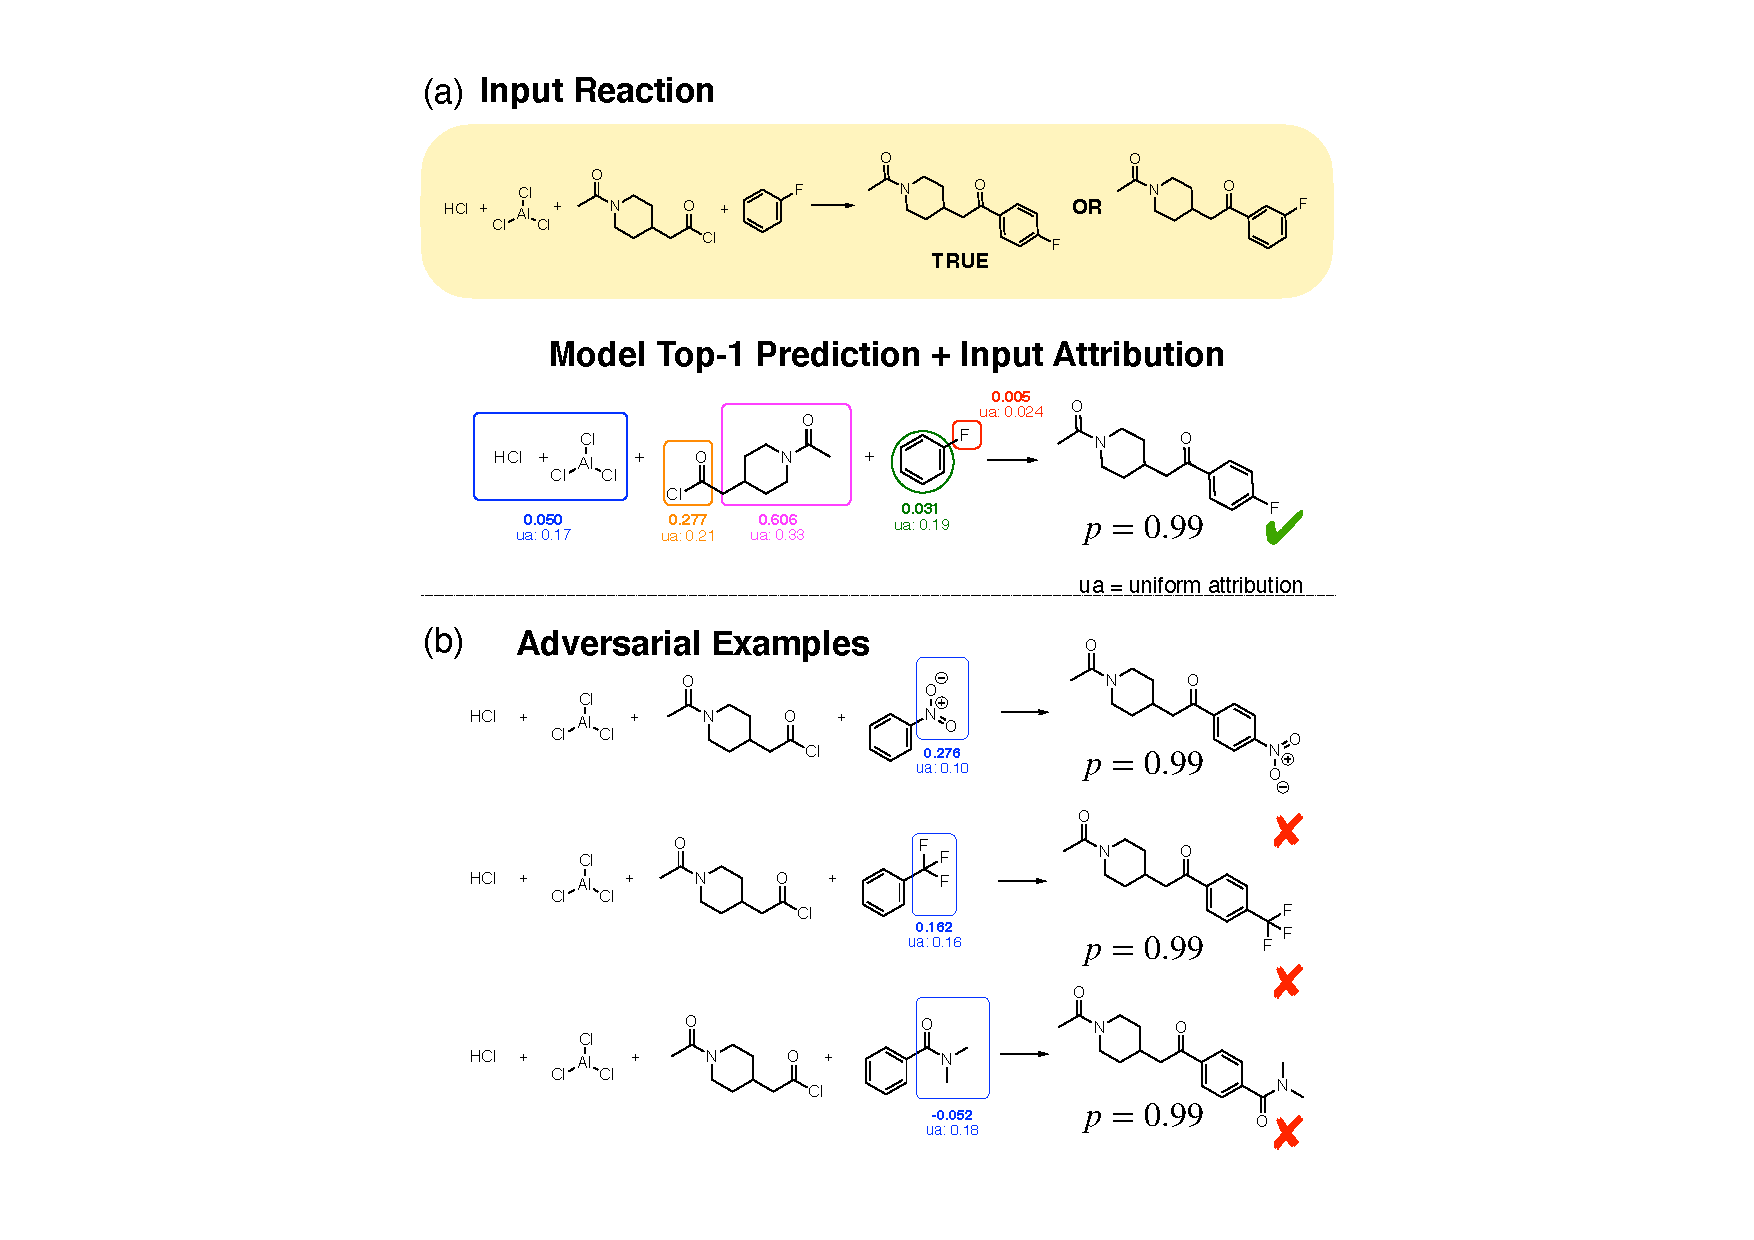
\includegraphics[width=0.6\textwidth]{Chapters/Transformer/Figs/sear.pdf}
    \caption{\label{fig:sear} \textbf{IG attributions reveal incorrect reasoning and guide the design of adversarial examples.} (\textbf{a}) The model correctly predicts the major para product of a typical Friedel-Crafts acylation, but low attribution is given to the para-directing -F group. (\textbf{b}) The model is fooled into incorrectly predicting the para product when the -F is replaced by meta-directing groups. The low attributions given to the directing groups indicate that the model has not learnt their importance.}
\end{figure}

Friedel-Crafts acylation reactions are an example of electrophilic aromatic substitution \cite{Friedel1877}. In these reactions a hydrogen on an aromatic ring is substituted by an acyl group. In the case of a benzene ring with a single substituent, there are three different hydrogen positions where this substitution can happen. The electronic and steric character of the substituent on the ring determine the selectivity of these reactions. An example of a selective Friedel-Crafts reaction is shown on Figure~\ref{fig:sear}(a) where according to the patent the para product is formed with a yield of 90\% \cite{fc_para1981}. In this reaction that acyl group is primarily substituting the hydrogen in the para position compared to the -F substituent. The transformation is correctly predicted by the Molecular Transformer. 

The IG attributions indicate that the importance of the fluorine (-F) for this reaction is completely neglected by the model. A much larger attribution is given to the reagent suggesting that the model attributes this selectivity to the reagent rather than the true directing group. Guided by the attributions we replaced the fluorine by a number of typical meta directing groups to create adversarial examples. We observe that the model (wrongly) predicts the para product. In this case negative attributions favour the meta product and positive attributions the para product. We do not find any correlation between the attribution values and the directing effect of the substituent. From this we can conclude that the model has not learnt the selectivity in the case of Friedel-Crafts acylation reactions on substituted benzene rings. 

\section{Revealing the Effect of Bias through Artificial Datasets}
Interestingly in one of the adversarial examples the attribution on the meta directing group is negative, meaning that according to the model the amide group (correctly) favours the formation of the meta product. This agrees with chemical principles, but the model is nonetheless still predicting the para to be the major product. We hypothesize that this might be due to biases in the training data -- using template analysis to count the number of para/meta/ortho Friedel-Crafts Acylations in USPTO (Figure~\ref{fig:venn_friedel}), we find that there are many more para substitution reactions than meta in the training dataset. This could result in the model being biased towards predicting para substitutions even in the presence of meta directing groups, as the model can achieve very high ($\sim 98\%$) accuracy on the training set by always predicting the para product.

\begin{figure}[htb!] 
    \centering    
    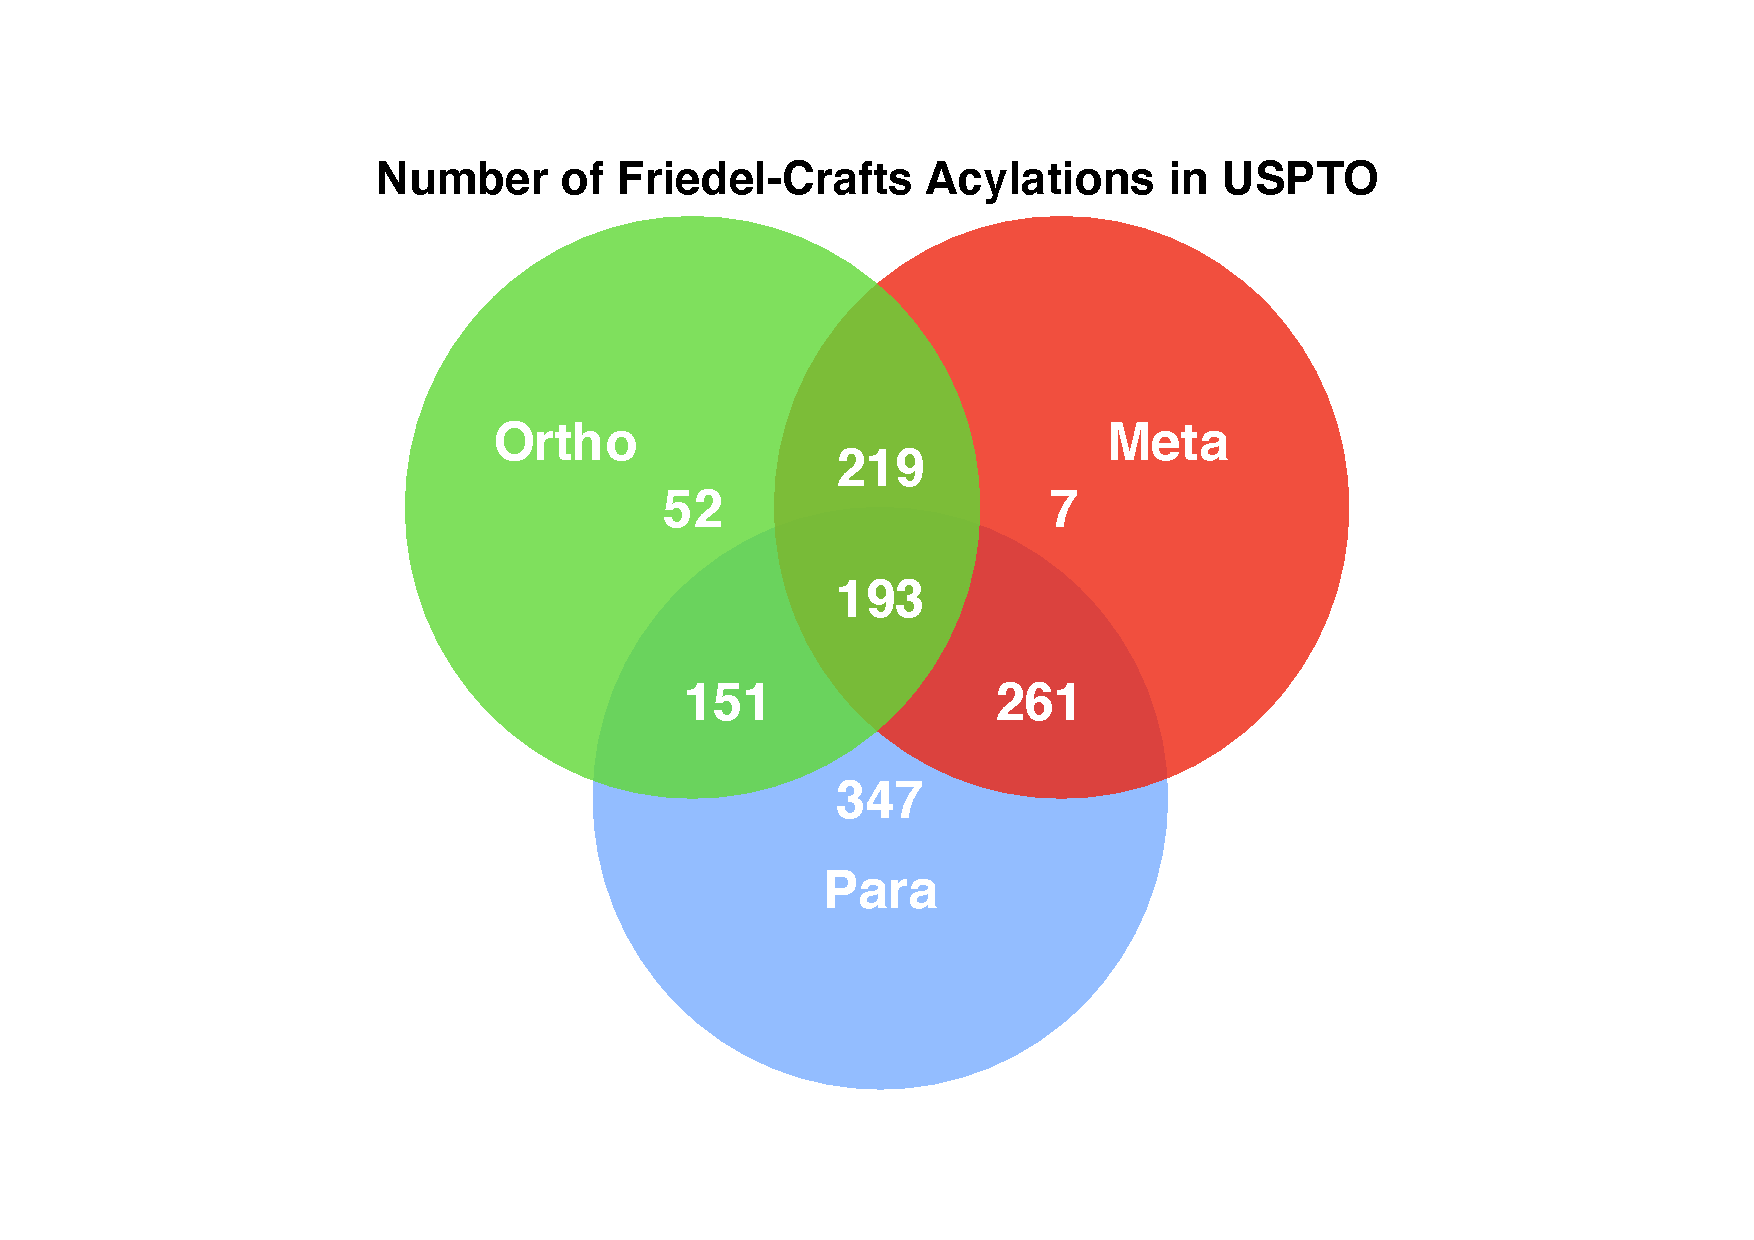
\includegraphics[width=0.5\textwidth]{Chapters/Transformer/Figs/venn.pdf}
    \caption{ \textbf{The number of para Friedel-Crafts acylation reactions in USPTO far outweigh those of meta or ortho reactions.} Overlaps in the Venn diagram denotes cases where the benzene has more than 1 substituent.}
    \label{fig:venn_friedel}
\end{figure}

To more quantitatively investigate how this imbalance in training data affects the model predictions, we train the Molecular Transformer on artificial datasets with varying proportions of meta and para Friedel-Crafts substitutions. By comparing the performance of the trained models, we demonstrate that the unchemical para-favouring behaviour of the USPTO-trained Molecular Transformer is the result of dataset bias.

% In light of the identified pathologies, we re-examine the reported 90\% accuracy of the Molecular Transformer and demonstrate that it is partly the result of scaffold bias in the dataset. We propose a new train / test split that is free from this bias, and show that the performance of the Molecular Transformer, We also show that the same issue exists for graph models as well by retraining the best reported graph model and observing a similar drop in accuracy.  

\subsection{Artificial dataset construction}
We generate three sets of artificial training data and one held-out artificial test set of electrophilic aromatic substitution reactions using SMART templates. Each reaction consists of a benzene ring singly substituted with a directing group reacting with an acyl chloride to form either a para- or meta- acylated product. 

Ten para directing groups (fluorobenzene, chlorobenzene, isopropylbenzene, tert-butyl\-benzene, N-phenylacetamide, N-phenylpropionamide, phenol, ethoxybenzene, isopropoxybenzene, sec-butyl\-benzene) and ten meta directing groups (N,N,N-trimethylbenzenaminium, (trifluoromethyl)benzene, benzaldehyde, acetophenone, methyl benzoate, ethyl benzoate, benzonitrile, nitrobenzene, methyl benzenesulfonate, ethyl benzenesulfonate) were used.

The -R groups for the acyl chlorides were generated by enumerating straight carbon chains of length 2-8 with 0-1 C=C double bonds also using SMARTS templates. Acyl chlorides were obtained by placing an acyl chloride group onto a random sp3 carbon on each of the -R groups. The acyl chlorides are enumerated with the benzyl compounds to generate valid chemical reactions. 

To investigate the effect of dataset bias, we vary the proportion of para:meta reactions in the training dataset and observe how the Molecular Transformer performs on a test set with an 1:1 proportion of para:meta reactions (Table~\ref{table:synth_datasets}). We first construct a `Balanced' dataset which has a 1:1 ratio of para:meta reactions (3100:3100) by enumerating all acyl chlorides with all benzyl compounds.  We also create a `Biased' dataset which has a 9:1 para:meta ratio (2790:310) by performing a 10:1 random split on the acyl chlorides so that less meta reactions are present. Finally we generate a `Severely Biased' dataset with 100:1 para:meta ratio (3000:30), which is closest to the observed ratio in USPTO, by performing a 33:1 random split on the acyl chlorides and also only keeping three meta-directing benzyl compounds (benzaldehyde, (trifluoromethyl)benzene, and nitrobenzene).

\begin{table}[hb!]
    \caption{\textbf{Number of meta-/para-directing reactions in the artificial datasets.}}
    \centering
    \label{table:synth_datasets}
    \begin{tabular}{m{0.3\textwidth}>{\centering}m{0.1\textwidth}>{\centering \arraybackslash}m{0.1\textwidth}}
    \toprule
      & \textbf{Meta} & \textbf{Para} \\ 
    \midrule
    Balanced (training) & 3100 & 3100  \\
    Biased (training) & 310 & 2790  \\
    Severely-Biased (training) & 30 & 3000  \\
    \midrule
    Test set & 177 & 177  \\
    \bottomrule
    \end{tabular}
\end{table}

The test set has an equal proportion of para and meta reactions generated using the three meta directing benzyl compounds from the `Severely Biased' training set and three para directing ones (Fluorobenzene, N-phenylpropionamide, and ethoxybenzene), together with -R groups from enumerating straight carbon chains of length 9-10 with no double bonds. This resulted in a test set with 177 para and 177 meta reactions.

\subsection{Model performance on artificial datasets}

On USPTO the Molecular Transformer was trained for $\sim$300 epochs, so for fair comparison this is the regime we wanted to investigate with the artificial datasets. We trained 10 transformer models on each of three training sets and saved checkpoints from the beginning of model training up to 256 epochs.

\begin{figure}[htb!] 
    \centering    
    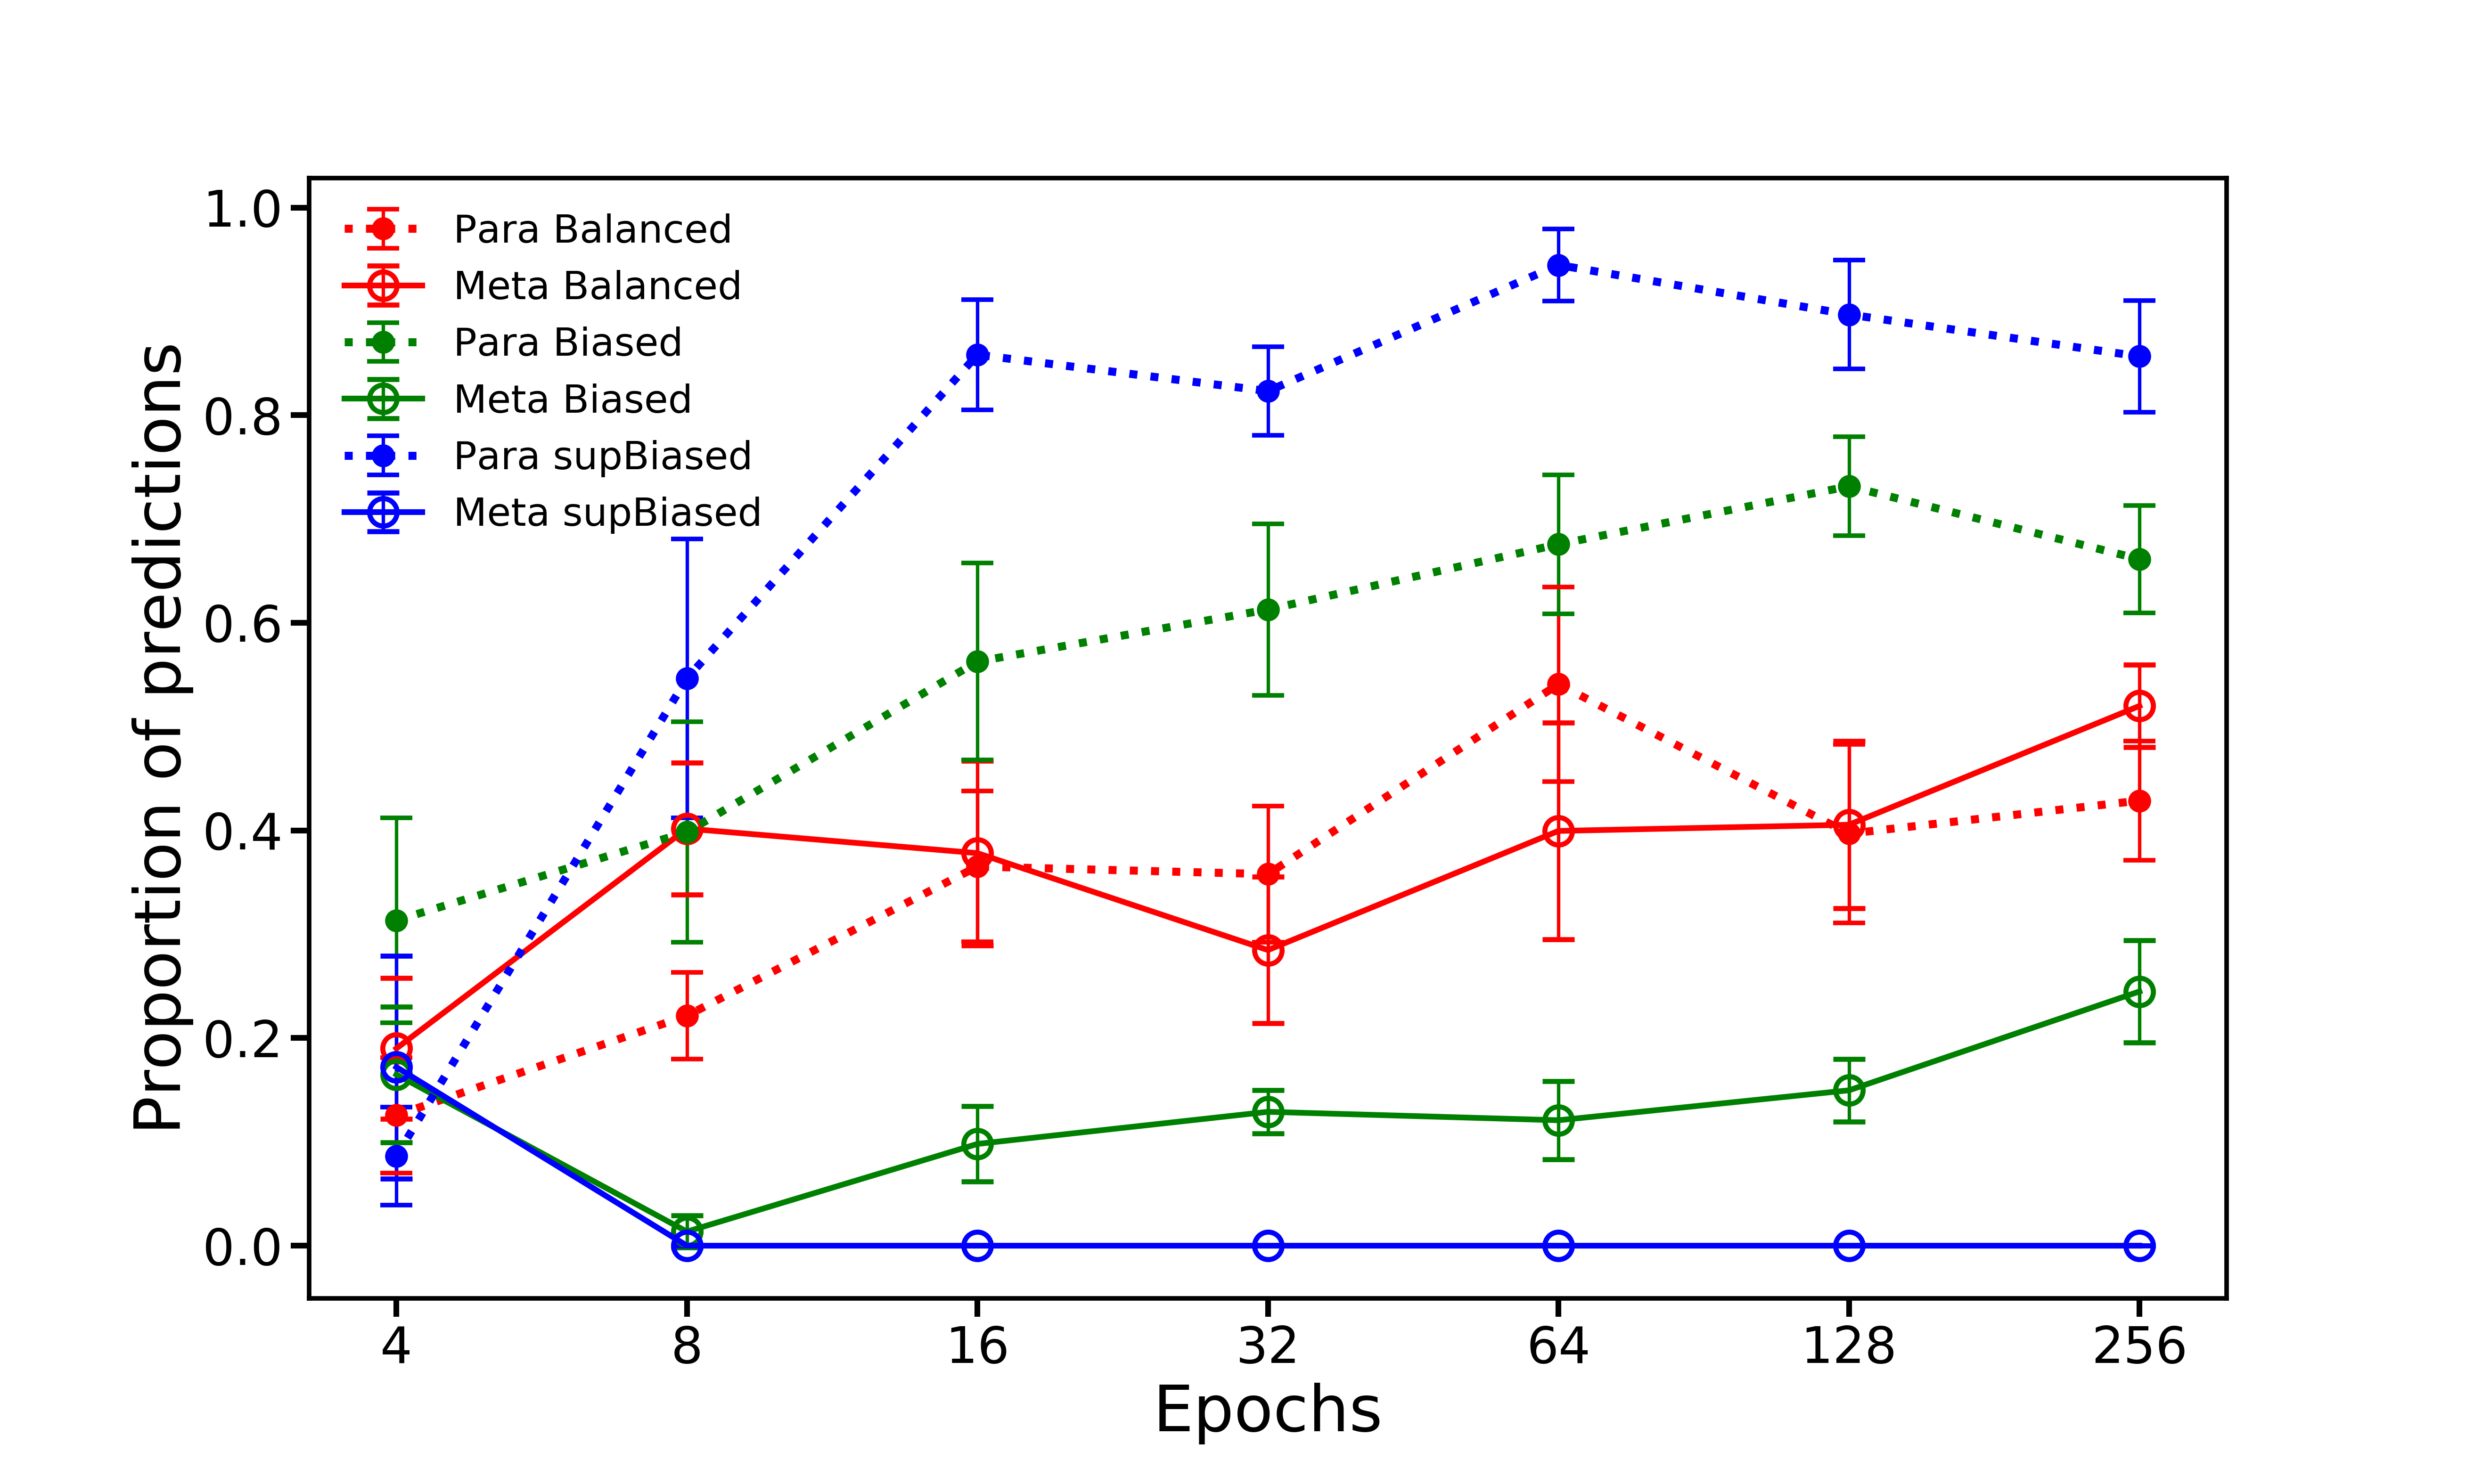
\includegraphics[width=0.8\textwidth]{Chapters/Transformer/Figs/synth_conv.png}
    \caption{ \textbf{Biased training data leads to biased predictions from the Molecular Transformer.} The figure shows the proportion of para (solid line) and meta (dashed line) predictions on a balanced test set as a function of the number of training epochs for different biased training sets. The error bars shown indicate the standard deviation in the results from training an ensemble of 10 randomly initialized models. The proportion of meta and para predictions does not always add up to 1, because it takes a number of iterations for the model to learn the SMILES syntax and we discount invalid predictions.}
    \label{fig:hamburger_plot}
\end{figure}


Using SMARTS template matching, we measured the proportion of model predictions (with valid SMILES) that are meta and para as a function of the number of epochs for different dataset biases (Fig~\ref{fig:hamburger_plot}). The results show that the Molecular Transformer is highly susceptible to learning dataset bias. When the model is trained on the balanced dataset, it rapidly converges to predicting equal amounts of para and meta substitution reactions, confirming that the bias is not caused by neural network architecture limitations. The model trained on the biased dataset containing only 10\% meta reactions in the training set is not able to get rid of the bias. For the severely biased training set (where the proportion of para/meta reactions are closest to the observed ratio in USPTO) the model does not predict any meta products at all.

Finally we ran the models to convergence to see if eventually they are able to predict the correct structures. After $\sim$4 000 epochs the ratio of meta to para was exactly 1:1 for the balanced dataset and about 3:5 on both the biased and severely-biased datasets. This shows that by training longer the effect of dataset bias can be mitigated, but it cannot be removed altogether. 

This numerical experiment confirms that the Molecular Transformer is guilty of the Clever Hans effect -- it appears to know chemical reactivity only because it learns hidden bias in the dataset. This is analogous to the bias observed in neural machine translation, where a pronoun indicates the gender of a word, but the model disregards it when making the translation due to the presence of gender stereotypes in the training data \cite{Stanovsky2019GenderBias}.

\section{Uncovering Scaffold bias}

Our case study of Friedel-Crafts acylation reveals the sensitivity of the Molecular Transformer to dataset bias. We turn to examine another source of bias -- compound series bias, or scaffold bias \cite{Mayr2018compare}. This is the phenomena where very similar molecules appear in both the training and the test set. This leads to ML models achieving high accuracy on the held-out set which does not necessarily correlate with the true generalization performance of the models. This is particularly acute for drug discovery datasets as medicinal chemists typically design molecular `series' by adding various functional groups to a central chemical `scaffold'. In chemical reaction datasets, scaffold bias manifest itself as similar molecules undergoing very similar transformations.

\begin{figure}[ht!]
    \centering
    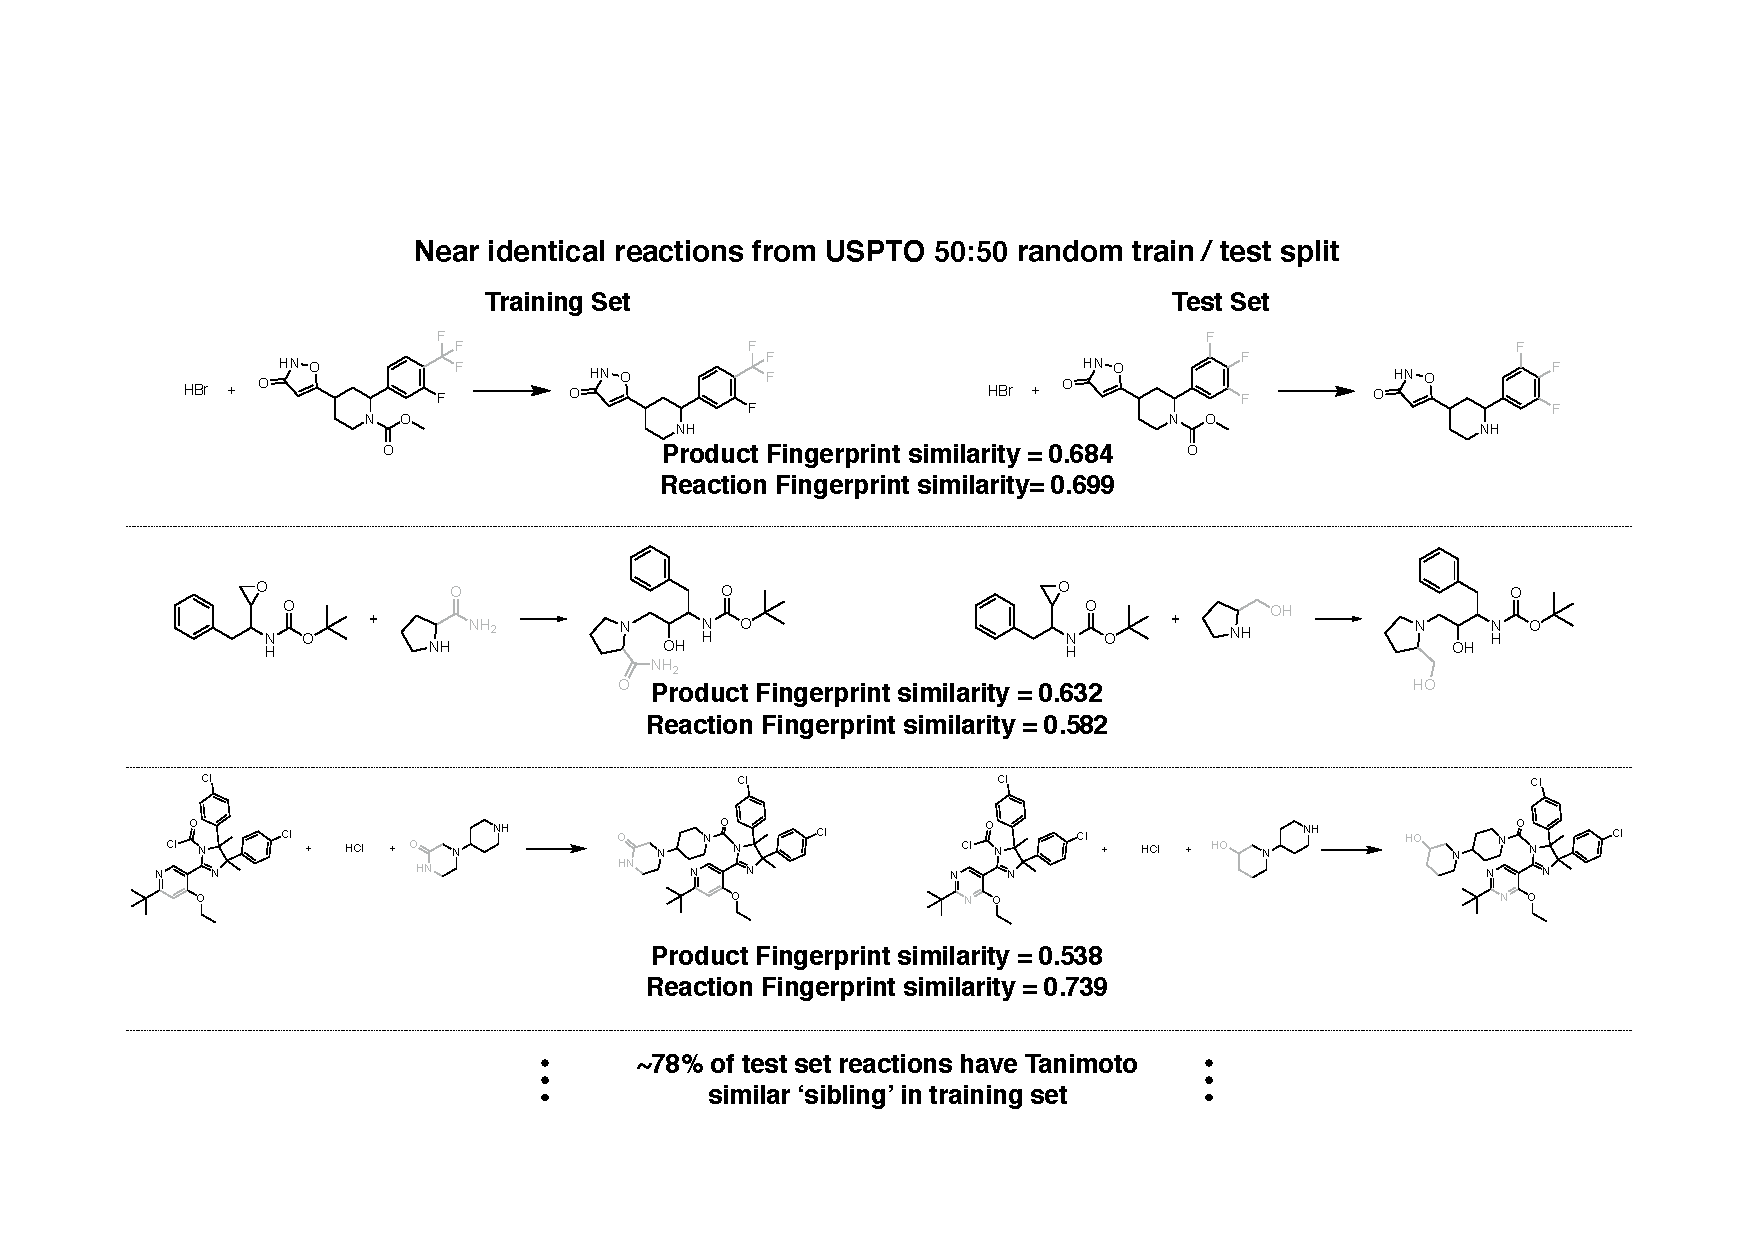
\includegraphics[width=\textwidth]{Chapters/Transformer/Figs/siblings_alt.pdf}
    \caption{\label{fig:sibling} \textbf{Randomly splitting USPTO results in a large number of near-identical reactions shared between train/test sets.}  $78\%$ of reactions in the test set have products that are within Tanimoto similarity $0.5$ of a product in the training set following a 50:50 random split. By eye it can be seen that many reactions with similar products (differences are highlighted by shading) have similar reagents and follow near-identical reaction mechanisms. This intuition is confirmed by the similarly high similarity of the reaction difference fingerprints from the reactions. The equivalent proportions are $93\%$ and $57\%$ for Tanimoto similarity $>0.4$ and $>0.6$, respectively.}
\end{figure}

To gain further insight into this phenomenon, we apply a 50:50 random train/test split to the full USPTO dataset and inspect reactions from one set that have structurally similar products to those from the other set. We define the 'structural similarity' of two molecules by calculating the Tanimoto similarity $\sigma$ between the Morgan fingerprints of the respective molecules \cite{Bajusz2015Tanimoto}. Figure~\ref{fig:sibling} reveals that many training and test set reactions are remarkably similar as measured by both $\sigma$ as well as the Tanimoto similarity of the reaction difference fingerprints of the reaction \cite{Schneider2015rxnfp}.

We find that 57\% to 93\% of reactions from the test set contain a structurally similar product to a reaction from the training set. This would not be problematic if the datapoints involved different reactants and reagents reacting via different mechanisms to form the same product. However this is not the case -- reactions with similar products often also share reactants and undergo similar chemical changes. This means that using a random train / test split to assess the performance of reaction prediction models could be a misleading indicator of their ability to generalize. Indeed, this reconciles the seeming contradiction between the reported 90\% top-1 accuracy of the Molecular Transformer and our findings above regarding the model's fragility to reactions involving chemical selectivity.

\subsection{Tanimoto-Splitting USPTO}

To account for this drastic scaffold bias, we propose that datasets for training machine learning reaction prediction models should be split by the Tanimoto similarity of the molecular fingerprints of the reaction products. In other words, it should be ensured that no reactions in the test set have a product that is within Tanimoto similarity $\sigma$ of any product from a training set reaction.

We implement this by first conducting a random split of the dataset, and then transferring all reactions that violate the Tanimoto similarity criteria from the test set to the training set -- the proportion of the initial random split is adjusted until the desired final train/test ratio is obtained. For USPTO with Tanimoto threshold $\sigma=0.6$, the dataset was randomly split 70\%:30\% and the ratio after Tanimoto splitting was 89.1\%:10.9\%. For the $\sigma=0.4$, the initial dataset was randomly split 30\%:70\% and the ratio after Tanimoto splitting was 91.7\%:8.3\%. 

The intent of such a dataset split is to remove structural bias but we must also make sure that the distribution of different reaction types in the train and test sets is still similar. This is important because we would like the test set score to reflect how well the model learnt the chemistry contained in the training set and we are less interested in extrapolation to unseen reaction types. To characterize the new Tanimoto-split dataset we inspected the distribution of reaction types in the training and test sets for both the random and Tanimoto-split datasets (Fig~\ref{fig:rxn_dist}). 

\begin{figure}[ht!]
    \centering
    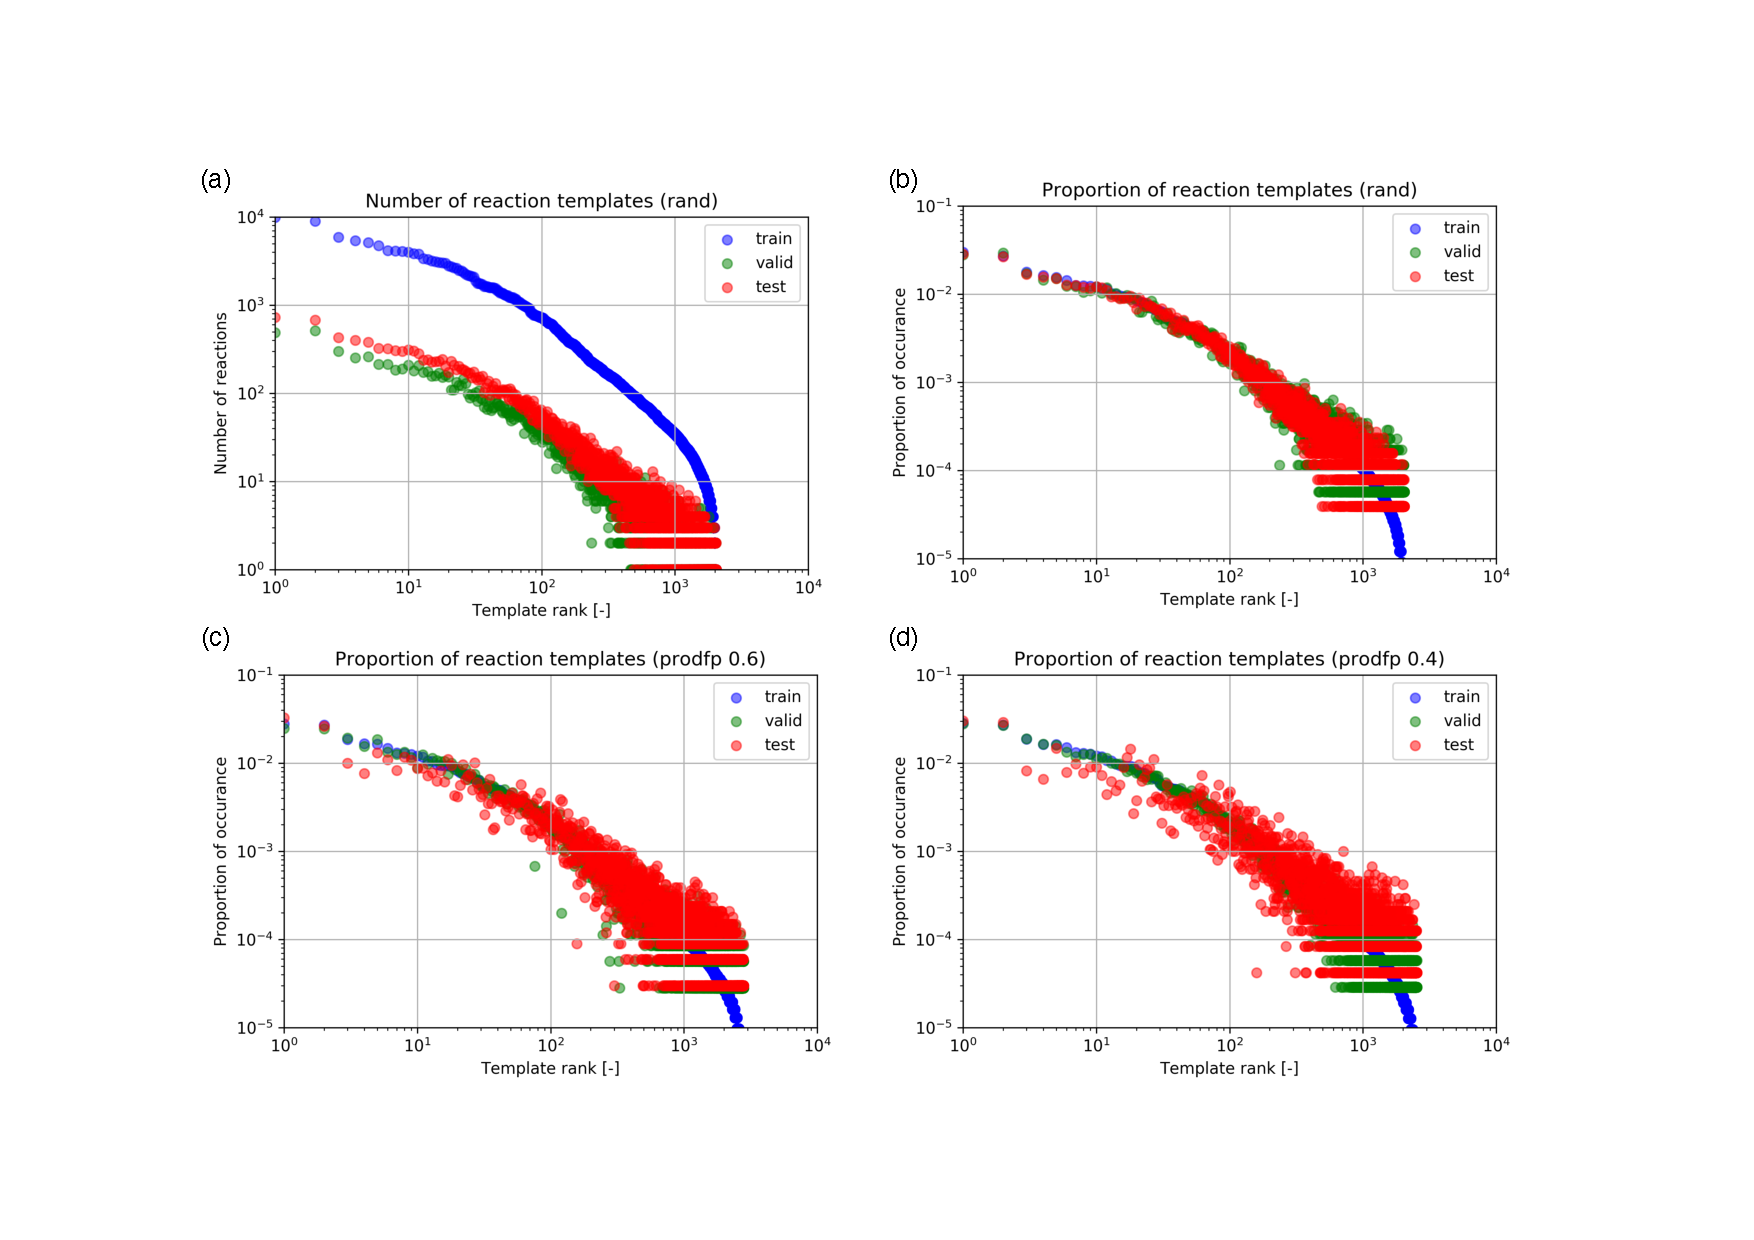
\includegraphics[width=\textwidth]{Chapters/Transformer/Figs/rxn_distribution.pdf}
    \caption{\label{fig:rxn_dist} \textbf{Tanimoto splitting minimally affects reaction template distribution.} (\textbf{a} - \textbf{b}) The absolute occurrence (\textbf{a}) and fractional occurrence (\textbf{b}) of reaction templates in train/valid/test sets of USPTO from a random split. The distribution of test set reactions closely resembles that of the validation set. (\textbf{c} - \textbf{d}) The fractional occurrence of reaction templates in train/valid/test sets of USPTO from two different Tanimoto splits using the Morgan fingerprint of the reaction product. As the Tanimoto similarity threshold value is tightened from 0.6 (\textbf{c}) to 0.4 (\textbf{d}), the deviation in frequency of the test set reactions from the training set increases.}
\end{figure}

In order to inspect how the distribution of reaction types changes when using fingerprint similarity-based splitting, open-source template extraction code~\cite{Coley19WLDN5} was applied on the training, validation, and test sets from different dataset splitting methods (Fig~\ref{fig:rxn_dist} (a)). Reaction SMARTS describing bond changes of radius 1 were used to classify reactions to particular templates. The frequency of occurrence for each reaction template is divided by the size of the training/validation/test set to obtain the fractional occurrence of the template, which is plotted in decreasing order of frequency in the training set. For rare templates (ie low frequency reaction types) floating point errors are encountered; however these do not affect the qualitative trends observed.

These graphs show that distribution of templates in the test set closely follows that of the training set in all cases (Fig~\ref{fig:rxn_dist} (b - d)). As increasingly strict fingerprint similarity-based splitting is applied, the fractional occurrence of rare templates deviates more and more from that of the training set. In addition, for both random and Tanimoto-splits there are no reaction templates present in the test set that are not contained in the training set, i.e. all reaction types in the test set are 'seen' by the model during training. In fact, Tanimoto-splitting increases the number of unique templates in the test set from $\sim$3k to $\sim$4.9k, suggesting that this splitting method can produce test sets that better represents the distribution of reaction types from the full dataset ($\sim$26k templates) compared to a random split. This is similar to an importance sampling scheme that helps sampling the tails of the distribution as well.

We also inspected using the fingerprint difference between the product and reactant molecules for calculation of Tanimoto similarity calculation, which led to qualitatively similar changes in the reaction template distribution. However, we have concerns that noise present in the data-mining of reactants and reagents (presence/absence of salt/catalysts/solvents etc) could cause unintentional effects on similarity calculation using reaction fingerprints and lead to additional hidden biases within the split. Together with the relative interpretability of the product fingerprint, we believe it is most practical to the community to simply use the molecular fingerprints of the reaction products for similarity calculation in splitting datasets.

\subsection{Model performance on Tanimoto-split USPTO}
We train and evaluate the Molecular Transformer on Tanimoto-split USPTO with $\sigma = 0.6$ and $\sigma = 0.4$, as well as the WLDN5 model of Coley et. al.~\cite{Coley19WLDN5} which is a widely-used graph-based machine learning reaction prediction model. This model explicitly represents molecules as graphs and considers reactions as series of graph edits instead of the Molecular Transformer's text-based translation of SMILES strings.

Table~\ref{table:tanimoto} shows that the model performance of both the graph-based model and the Molecular Transformer significantly decrease upon debiasing the dataset, but Molecular Transformer continues to outperform WLDN5.  These results show that scaffold bias affects both graph-based and sequence-based models, confirming that this bias is intrinsic to data and independent of model architecture. Importantly, this demonstrates that there is significant scope for improvement in the performance of reaction prediction, and that the 90\% accuracy obtained for a randomly split dataset does not necessarily translate to real-life applications.

\begin{table}[!h]
    \centering
    \caption{ \textbf{Reaction prediction models are strongly affected by scaffold bias.} The performance of the Molecular Transformer and WLDN5 on various USPTO train/test splits are shown, with the accuracy of the best-performing model highlighted in bold.}
    \centering
    \label{table:tanimoto}
    \begin{tabular*}{0.8\textwidth}{l@{\extracolsep{\fill}}rrr}
    \toprule
        \textbf{Model} & \textbf{Top-1[\%]} & \textbf{Top-3[\%]} & \textbf{Top-5[\%]}\\ 
        \midrule 
    & \multicolumn{3}{c}{Original} \\
    \midrule
    Molecular Transformer & \textbf{90.4\%} & \textbf{94.6\%} & \textbf{95.3\%}  \\
    WLDN5 & 85.6\% & 92.8\% & 93.4\%  \\
    \midrule 
    & \multicolumn{3}{c}{Tanimoto Similarity \textless\,0.6} \\
    \midrule
    Molecular Transformer & \textbf{80.9\%} & \textbf{88.2\%} & \textbf{89.6\%}  \\
    WLDN5 & 75.9\% & 86.2\% & 88.8\%  \\
    \midrule
    & \multicolumn{3}{c}{Tanimoto Similarity \textless\,0.4}\\
    \midrule
    Molecular Transformer & \textbf{74.6\%} & \textbf{82.9\%} & \textbf{84.5\%} \\
    WLDN5 & 69.3\% & 80.9\% & 84.1\% \\
    \bottomrule
    \end{tabular*}
\end{table}

\section{Discussion}
% Chemical reaction prediction models have undergone a revolution driven by innovations in the field of machine learning. This large increase in accuracy came at the expense of interpretability as expert crafted rules and reaction mechanisms gave way to black-box deep learning models. 

% The predictions of machine learning models depend on two essential components. One of them is the training data which acts as an upper limit to the performance of the model. Any machine learning model can be only as good as the data it was trained on. The other ingredient is the input that is processed and turned into the prediction. We have developed two robust methods for interpreting and testing reaction prediction models focusing on each of these two ingredients, and applied them to analyse the Molecular Transformer which is the current state-of-the-art model. 

% The first method builds on the Integrated Gradients method \cite{Sundararajan2017AxiomaticNetworks} for attributing the prediction of neural network models to parts of the input. This method has been used to identify which parts of the inputs to the model are important when predicting typical selective chemical reactions. It has been found that often the model does not identify chemically important substructures, demonstrated by the design of adversarial examples based on the attributions which fool the model.

% The other method we developed attributes the predictions of the model to training data. We averaged the vector outputs from the last encoder layer of the Molecular Transformer to define a similarity metric between different reactions, as understood by the model. Attributing back to training data serves multiple purposes in the case of reaction prediction. It can either support or invalidate a prediction by telling the user which are the most similar training reactions according to the model. Furthermore this can be used to identify unknown trends or biases in the dataset or sometimes even to identify erroneous training examples. 

% Using evidence from these attribution methods, we hypothesized that many of the erroneous predictions of the Molecular Transformer model stem from data biases. We have validated this hypothesis by designing an artificial dataset of Friedel-Crafts acylation reactions where we could show how biases in the dataset manifest in the predictions of the model. In addition, we observe that the model trained on the Pistachio dataset had in general better predictions and much better calibrated uncertainty scores, in spite of the fact that this model only achieved 76\% test-set accuracy. This suggests that Pistachio is not as biased as USPTO, and hints that the addition of training data can substantially improve model performance. 

% From these results we believe that for reaction prediction, the Top-$N$ accuracy from testing on randomly chosen held-out test sets do not provide an adequate measure of the models true performance and generalization ability. We believe that this is partly results from the fact that publications and patents often contain reaction carried out on a series of analogous reactants. Therefore there is a high chance that essentially identical reactions end up in the training and test sets. A more honest measurement of the model's true generalizability could be realized by only including reactions in the test-set whose products have a low similarity to the products in the training set. The exploration of this idea is the subject of further work. 

% Overall, from this work we believe that improvements to the training data can be just as impactful as improving the machine learning models themselves. By demonstrating the power of interpretability methods when rigorously applied to scientific questions, we have shown that these methods can be useful beyond just giving explanations of predictions by exposing dataset biases. Applying our approach for data and input interpretation beyond chemical reaction prediction to other fields will likely be equally constructive, illuminating the path to improved training data and hence improved artificial intelligence models.

In this chapter we developed a framework for quantitatively interpreting the predictions of Molecular Transformer, a state-of-the-art model for predicting the outcome of chemical reactions. We show that the model makes predictions based on patterns it recognizes and the statistics of the training data, but this does not necessarily coincide with the underlying chemical drivers of reactivity. This can result in erroneous predictions. Attributing the predicted probability to parts of the input allowed us to foresee these failure modes. 

Through this interpretation framework, we discover that the model is susceptible to the Clever Hans effect, where the correct outcome is reached by learning bias. For instance, the dataset contains orders of magnitude more para than meta electrophilic aromatic substitution reactions, and the Molecular Transformer frequently arrived at correct test set prediction by simply memorising this fact. We believe that the inclusion of additional physical insight into models, as done in recent work incorporating explicit reaction mechanisms for reaction prediction \cite{bradshaw2019generative} and machine-learning regio-selectivity prediction \cite{guan_coley_robust}, could be an effective way of increasing model robustness against dataset bias. A possible way to accomplish this in Transformer models is via the augmentation of token embeddings with physical descriptors. Moreover, future efforts should focus on benchmarking other graph-based synthesis prediction tools such as the recent MEGAN architecture as well \cite{sacha2020molecule}.

We have also shown that incorrect predictions can be the result of erroneous training data points. This can be revealed using our method to attribute model predictions to training data. This method can also aid experimental chemists using the Molecular Transformer. The references corresponding to the most similar training reactions can be used to impute experimental conditions. This principle can be used in many scientific machine learning applications where the training data is generated via text-mining which is known to lead to loss of important meta data, like reaction conditions. 

Finally we have shown that scaffold bias is a phenomena present in the published literature on reaction prediction. Many of the reactions in the test set have almost identical twins in the training set. This leads to an overestimation of the generalization performance of the models as reported in the literature. We have re-trained two of the leading models the Molecular Transformer and the graph-based WLDN5 model on our new Tanimoto-split dataset and found that the Top-1 accuracy of the models dropped significantly.

Our work highlights the importance of understanding and evaluating scientific machine learning models beyond looking at their accuracy on standard benchmark datasets. By rigorously applying interpretability techniques, we reveal how systematic weaknesses of the models can be uncovered, proving insights that facilitate the work of model developers. We believe further work into the use of input attribution and interpretability tools to critically analyse machine learning models for retrosynthesis, as well as other areas of computational science, is vital and necessary for continued refinement of predictive models.

% % ChatGPT
% Chemical structure biases can arise in SMILES-based language models for retrosynthesis prediction due to a variety of factors, such as limitations in the available training data, the choice of molecular descriptors used to represent compounds, and biases in the reaction data used to train the models. However, there are several potential approaches for reducing such biases and improving the performance of SMILES-based language models for retrosynthesis prediction.

% One approach is to use a diverse set of training data that covers a broad range of chemical structures, including compounds with diverse functional groups, stereochemistry, and ring systems. This can help to reduce biases that may arise from over-representing certain chemical structures or functional groups in the training data, and can improve the generalizability of the model to new and unseen compounds.

% Another approach is to use a variety of molecular descriptors to represent chemical structures in the training data, rather than relying solely on SMILES strings. This can help to capture a more complete representation of chemical structure and can reduce biases that may arise from limitations in the SMILES notation, such as the inability to represent certain types of stereochemistry or complex ring systems.

% In addition, it may be possible to reduce biases in the reaction data used to train the models by carefully curating the data set to include a diverse set of reaction types and conditions, and by incorporating data from a range of sources, such as academic publications, patents, and commercial databases.

% Finally, it is important to recognize that biases can also arise from the model architecture and training process itself, and therefore, it is important to carefully monitor and evaluate the model performance and make adjustments as necessary to reduce any biases that may arise.

% Overall, reducing biases in chemical structure from chemical reaction data used to train SMILES-based language models for retrosynthesis prediction is an ongoing and challenging problem, but with careful consideration of the training data, molecular descriptors, and model architecture, it may be possible to develop models that are more robust and generalizable to a broad range of chemical structures and reaction types.

% % \section{Introduction}
% % \label{sec:int}
% % Although the design of drug candidates is exhaustingly difficult, it is in fact the `make' part of the design-make-test cycle which is the most costly, time consuming and labour intensive. The key to streamlining molecular synthesis is in improving route planning, developing faster ways of designing shorter reaction paths from basic molecular building blocks to the desired molecule, reducing the number of steps and hence the risk of failure.

% % Once a synthesis route is designed it is important to validate each step of the plan. Forward chemical reaction prediction is concerned with predicting the (major) product of an organic reaction given the reactants, reagents and preferably the conditions like solvent, temperature, concentrations etc. By having the ability to predict the product of reactions with reliable uncertainties it is possible to design clever synthesis plans where the reactions with higher uncertainty are put first. This way if a synthesis protocol fails it does so fast and cheap instead of in the later stages of the route where substantial time and cost would go to waste.

% % Route planning and reaction prediction have traditionally been done by expert chemists relying on experience, as well as reaction databases like Reaxys \cite{ElsevierReaxysDatabase}. Nowadays, Computer Assisted Synthesis Planning tools are increasingly being used \cite{Coley2018}, as these tools can memorise libraries of commercially available building blocks and quickly evaluate large numbers of possible bond disconnections via efficient algorithms such as Monte Carlo Tree Search \cite{Segler2018PlanningAIb}. Unsurprisingly, machine learning methods have also entered into the fray \cite{Coley2019AutonomousOutlook, Coley2019AutonomousProgress} and have recently emerged as the most successful approach \cite{Coley2018, Schwaller2019MolecularPrediction}.

% % ML reaction prediction models are trained on reaction data that is extracted from patents and publications. In these documents usually the metadata about reactions like the temperature, concentrations and solvents are found in the synthesis protocol section making it very challenging to extract this information in an automated manner. Therefore these models are usually trained only on the reactants and reagents with all of the context information missing. In spite of this there are reported models achieving remarkably high near 90\% Top-1 prediction accuracy on these datasets, even outperforming quantum mechanics-based approaches \cite{Schwaller2019MolecularPrediction}. 

% % The natural question that arises is: how is the model able to achieve such high accuracy on often rather challenging reactions from such limited source of data? Has the model learnt the well-established underlying mechanistic drivers of reactivity purely from data? It is of utmost importance to validate these models to see if they are able to generalize and predict the outcome of reactions reliably or if they are merely learning hidden biases in the datasets which results in the seemingly strong performance. 

% % One way to accomplish this is with ML interpretability methods \cite{Alvarez-Melis2018OnMethods}. Interpretability methods can help uncover the reasoning of model predictions in simple well understood cases where the physical or chemical cause for certain outcomes is well established. For chemical reaction prediction our understanding of mechanisms and selectivities serves as good guides for the observed reactivities.

% % In this work, we use a well-known ML interpretation method called Integrated Gradients (IGs) to probe the understanding of the Molecular Transformer (MT), the current state-of-the-art machine learning model for chemical reaction prediction. Our approach builds on the work of McCloskey et.\,al.\,\cite{McCloskey2019UsingChemistry} who used IGs to understand binding prediction models on artificial datasets. We extend the method to Transformer architectures, and use it in the context of reaction predictions on real experimental data. We also present a novel method for attributing the predictions of neural network models to training set datapoints. With these tools we show that MT often fails to learn the mechanistic reasoning behind chemical selectivity and hypothesize that this is due to hidden biases in the dataset. We justify this claim by creating biased synthetic datasets and demonstrating selectivity bias in the model predictions, suggesting that it is the quality of training data rather than the particulars of model architectures that is constraining the potential for ML reaction prediction.


% % The second dataset used was the commercial Pistachio dataset \cite{Mayfield2018Pistachio2.0}. This dataset contains over 9 million reactions text mined from US and EPO patents. This dataset was filtered similarly to USPTO to remove erroneous and and a large number of duplicate reactions. The final dataset consisted of 2 375 385 reactions, of which 2 019 078 were used for training, 118 770 for validation and 237 537 for testing. 

% % The model trained as described above achieved 76.4\% Top-1 accuracy on the test set. Even though this looks like a substantially lower performance in reality the two models perform similarly well on new reactions. The possible reasons for the large difference in the measured performance on the held-out test sets are described in detail below. This model obtained was also used in the interpretability experiments to test the effect of increased training set size on the models understanding of chemistry and is referred to as Pistachio Transformer from here onwards. 

% % \subsection{Integrated Gradients}
% % To understand the predictions of MT with respect to the input features, we use the Integrated Gradients \cite{Sundararajan2017AxiomaticNetworks} attribution method. Integrated Gradients (IGs) is a principled model-agnostic feature attribution method adapted from game theory which obeys certain axioms of fairness. It can be used for any model where gradients are available, which is the case for all neural networks that are trained by some variant of gradient based optimization.

% % In general, the attribution of feature $i$ for input $x$ is given by
% % \begin{equation}
% % \label{eqn:IG}
% %     IG_i(x) = (x_i - x_i') \int_{\alpha=0}^1 \frac{\partial F(x' + \alpha(x-x'))}{\partial x_i} d\alpha
% % \end{equation}
% % where $x_i$ is the vector of feature $i$ for the input $x$, and $x_i'$ is a vector corresponding to a non-informative baseline input, $F(x)$ represents the model prediction for input $x$, and the integral is taken over the straight-line path from the baseline to the input of interest. 

% % It has been discussed before that the choice of baseline can have a large effect on the values of the attributions \cite{sturmfels2020visualizing}. While we could have chosen unreactive molecules as our baseline, it is important to select baselines which are completely non-informative to avoid any ambiguity. This would traditionally be the black image in the case of image recognition. In this work we use the embedding vector of the SMILES ` \textbf{.} ' token which is used to separate different molecules and hence does not contain any chemical information on its own.

% % For MT, we take great care to define $F(x)$ as it is not an appropriate question to ask what part of the reactant-reagent input is most important for predicting a given product. All of the input tokens contain crucial information that are used by the decoder to generate the entire target structure correctly. To eliminate this effect we define $F(x)$ as the difference in predicted probability of two possible products. Since the inert parts of the input are the same for the two products they should not substantially contribute to their predicted probability difference. This method is especially suited for examining reactions with selectivities. In other words we attribute the selectivity between two products to the inputs, ideally highlighting the chemically important groups driving this selectivity (by summing the attributions of the tokens comprising these groups).

% % If it is found that the correct product is predicted for the wrong reason i.e. the attribution on the chemical important group is low, it can be confirmed that model has not been able to learn the underlying chemistry through the construction of adversarial examples. In these examples we only change the parts that are chemically important, but not according to the model. This way the model can be fooled into incorrect predictions if the interpretation is correct, or the interpretation can be falsified if the model is able to predict the correct product. This is a crucial element of our method as any interpretation that cannot be falsified would be no more than speculation.

% % When talking about the size of an attribution we always compare it to the amount of attribution the group would get if the probability difference would be distributed uniformly across the input tokens. This serves as a way of normalizing the attributions by the size of the different substructures. We consider the parts of the reactant that get substantially higher attribution than expected to be `important'.

% % \subsection{Data Attribution}
% % In cases when a model predicts something very unexpected to humans attributions to parts of the input can be difficult to make sense of. Sometimes it can be much more illustrative to attribute to data instead and see a couple of example inputs that the model finds similar, which can reveal biases that the model has learnt.

% % To successfully attribute to data, we must understand how `similar' two input datapoints are according to the model by defining a similarity metric. For the Molecular Transformer which has an encoder-decoder architecture we use the output of the encoder layers as a basis for comparing data points. The challenge lies in the fact that these encoder hidden states have a non-fixed length $256\times N$ where $N$ is the length of the input sequence. To overcome this we average these vectors over the sequence dimension $N$, obtaining a representation of fixed size 256. We hypothesized that averaging can work because of the relatively large dimensionality and hence sparsity of the embedding space, allowing the averaged vector to retain most of the information about the structure, reagents and reactivity. 

% % We generated these averaged encoder state vectors for all of the reactions in the training sets. When a new example input is given it is passed through the Transformer encoder and the average hidden state vector of it is calculated. The similarity score of this vector to the training set vectors is calculated by
% % \begin{equation}
% %     score = \frac{1}{1 + D}
% % \end{equation}
% % where $D$ is the Euclidean distance between the vectors. This can be implemented in a vectorized way resulting in very quick computation even in the case of dataset sizes like Pistachio made up of over 2 million training examples. The top-$n$ most similar reactions are returned where $n$ is defined by the user. A similar approach is used in \cite{Allen2020} to measure the model-learned similarity between molecules for a graph neural network trained on toxicity prediction. These similarities are also used as evidence for judging the reliability of the model predictions, but only for unseen molecules not in the training set. In this work we go beyond assessing reliability into explaining the failures of the model by explicitly examining the training data itself to reveal hidden biases.

% % % From each reaction type we design a representative reaction that contained some selectivity and produce predictions with the USPTO and Pistachio Transformer. In the case of correct predictions the IG attributions were generated and evaluated whether they agreed with the underlying chemical causes of selectivity or not. After that based on the IGs a number of adversarial examples were generated to either confirm that the model is making the right prediction for the right reason or to confirm that the interpretation is correct and the model did not learn the underlying chemical causes. Attributions to training data were also generated to help confirm that the model is correctly making predictions based on chemically similar examples and also to help identify the causes of incorrect predictions. The causes found include the absence of similar reactions in the training set, erroneous training datapoints and biases in the training set. 

% % \begin{figure}[htbp!] 
% % \centering    
% % 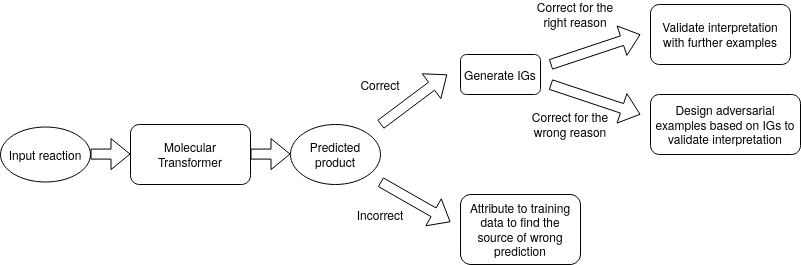
\includegraphics[width=1.05\textwidth]{Chapters/Transformer/Figs/workflow.png}
% % \caption[workflow]{An overview of the workflow for interpreting the Molecular Transformer.}
% % \label{fig:workflow}
% % \end{figure}

% % \section{Results}
% % To interpret the predictions of the Molecular Transformer we follow an analysis workflow (Fig~\ref{fig:workflow}) and examine a number of reaction types that are commonly used in synthetic organic chemistry using both input and data attribution techniques.
% % \subsection{Diels-Alder reactions}
% % The Diels-Alder reactions transform a conjugated diene and an alkene (called dienophile) to a six membered ring with a double bond \cite{Clayden2012}. A typical example is shown in Fig~\ref{fig:da1}. Diels-Alder reactions are regioselective meaning that the methoxy and nitrile group can be opposite or one carbon apart on the ring formed as shown in Fig~\ref{fig:da1}. The major product is the one marked TRUE on the figure because of more favourable HOMO-LUMO interactions. Due to the large number of possible products and complicated rules determining the major product the Diels-Alder reaction can serve as a challenging test for any reaction prediction model.

% % \begin{figure}[htbp!] 
% % \centering    
% % 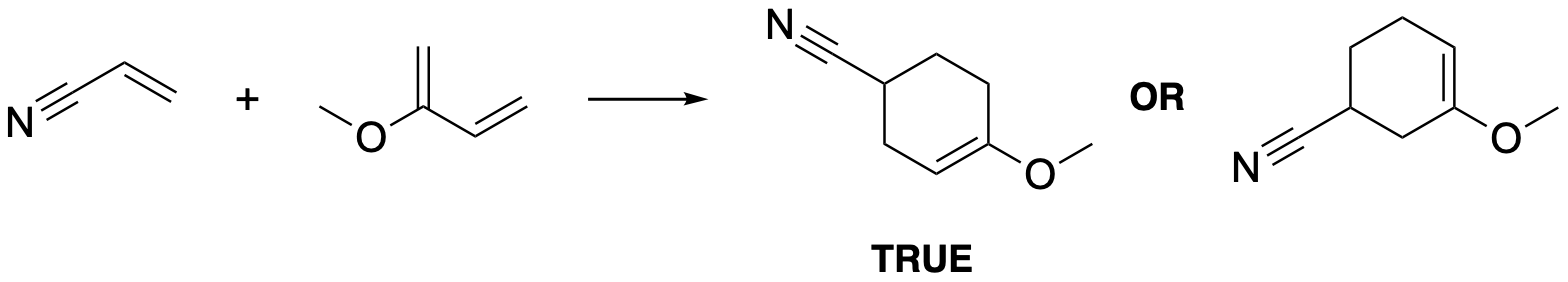
\includegraphics[width=0.9\textwidth]{Chapters/Transformer/Figs/da1.png}
% % \caption[Diels-Alder]{A typical example of a Diels-Alder reaction with challenging selectivity.}
% % \label{fig:da1}
% % \end{figure}

% % \begin{figure}[htbp!] 
% % \centering    
% % 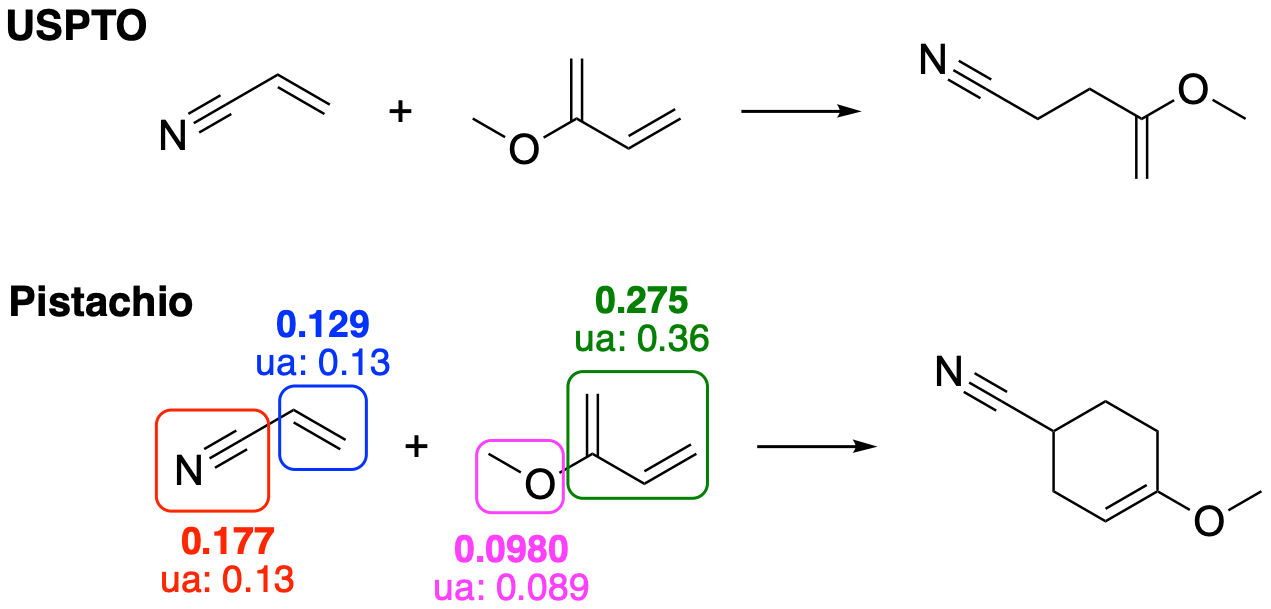
\includegraphics[width=0.8\textwidth]{Chapters/Transformer/Figs/da1_preds.png}
% % \caption[Diels-Alder]{The USPTO transformer makes a completely incorrect prediction, while the Pistachio model correctly predicts the product and recognises the importance of the nitrile group. For the Pistachio model the IG attributions are shown together with the corresponding uniform attribution (ua) values. }
% % \label{fig:da1_preds}
% % \end{figure}

% % Fig~\ref{fig:da1_preds} shows the Top-1 prediction of the USPTO and Pistachio models. The USPTO model does not seem to recognize the Diels-Alder reaction and gets the prediction wrong, indicating its own uncertainty by assigning a very low score of 0.300 to the prediction. To find the reason for the wrong prediction we attributed to training data (Fig~\ref{fig:da1_uspto_dat}). The first reaction seems to be an erroneous datapoint whereas the other two are different carbon-carbon bond formation reactions. This indicates that either the model has not learnt to recognize Diels-Alder reactions or the dataset did not contain any of them. 

% % \begin{figure}[htbp!] 
% % \centering    
% % 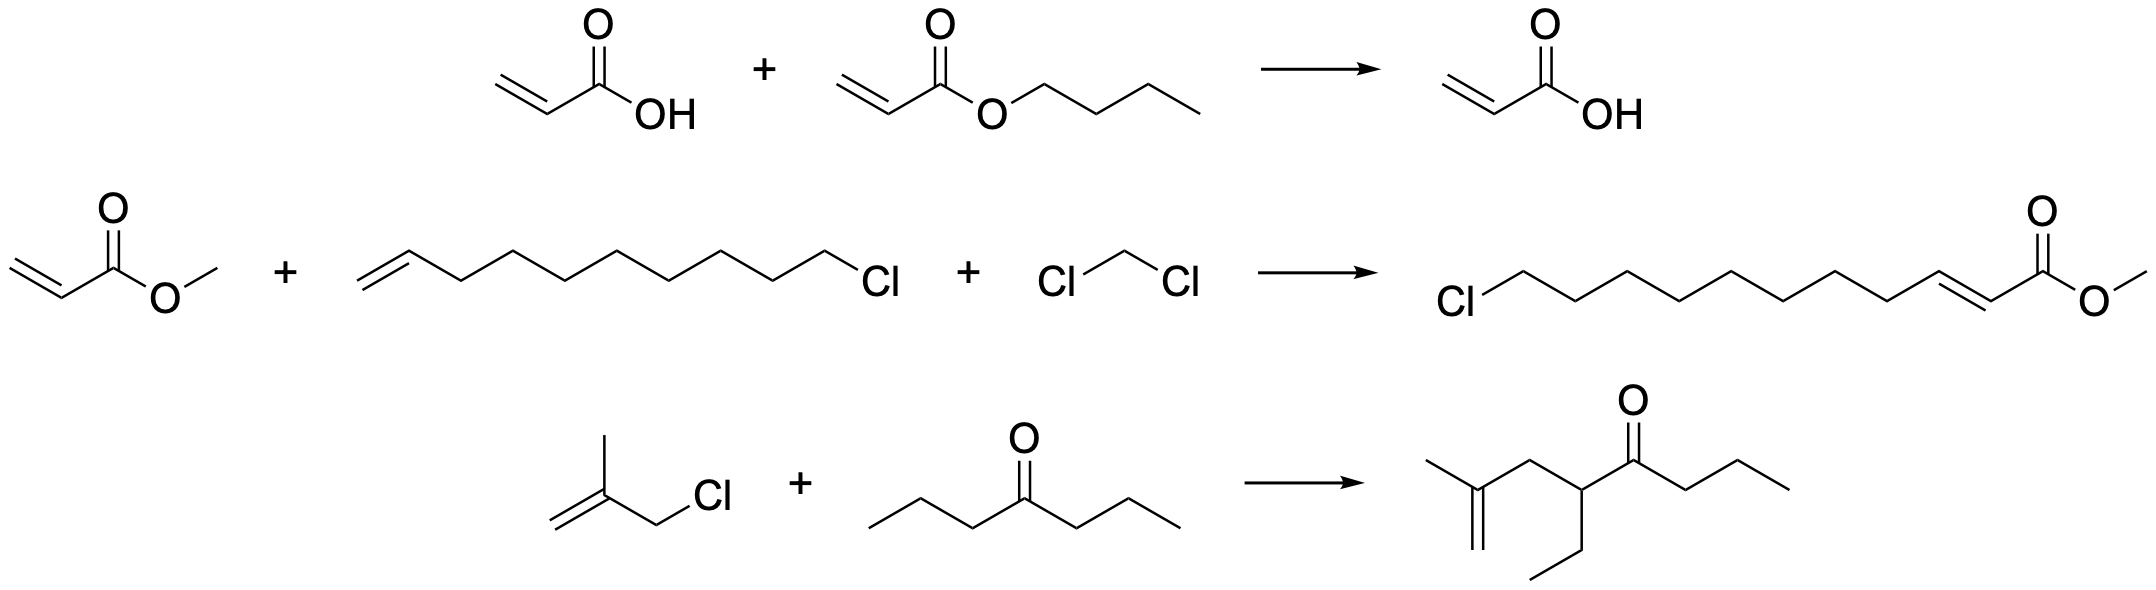
\includegraphics[width=1.0\textwidth]{Chapters/Transformer/Figs/da1_uspto_dat.png}
% % \caption[Diels-Alder]{Attribution to the USPTO training data shows that the USPTO transformer either completely fails to recognize Diels-Alder reactions or that no Diels-Alder reactions exist in the dataset. }
% % \label{fig:da1_uspto_dat}
% % \end{figure}

% % To check this we devised a simple reaction template of Diels-Alder reactions and ran a template matching algorithm on the training data. We validated the template by ensuring it was able to identify the reactions where a diene and a double bond participate in cyclo-addition, which made up 80\% of the $\sim$2.3k labelled Diels-Alder reactions in Pistachio. This template matched only 7 reactions in the USPTO dataset confirming that it contains very few instances of this type of reaction. Furthermore this suggests that the model was not able to generalize across chemical space to infer this reactivity from different types of reactions. This level of generalization could only be expected from physics based models that have direct access to quantum mechanical information driving the reactions.

% % \begin{figure}[htbp!] 
% % \centering    
% % 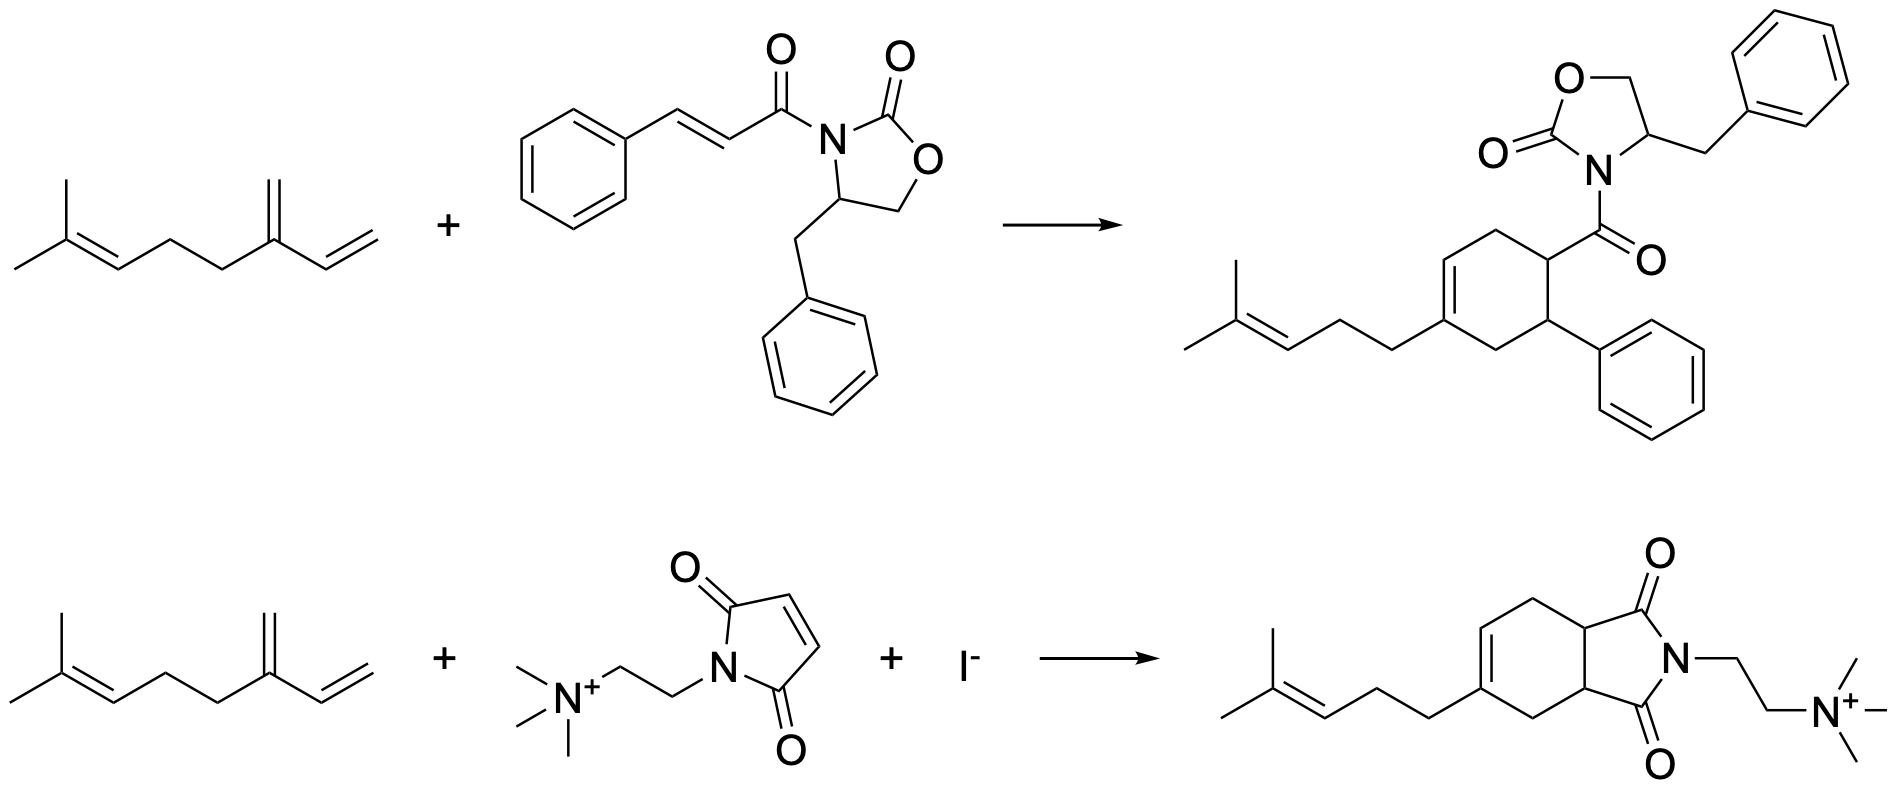
\includegraphics[width=1.0\textwidth]{Chapters/Transformer/Figs/da1_adv.png}
% % \caption[Diels-Alder]{Further test reactions correctly predicted by the Pistachio model, validate that Pistachio correctly understands Diels-Alder reactions. \cite{Husinec2011AnnulationsDerivatives, Tiamas2018AsymmetricChalcones}}
% % \label{fig:da1_adv}
% % \end{figure}

% % For the Pistachio model the Top-1 prediction is correct, as shown in Fig~\ref{fig:da1_preds}, and it has a confidence score of 0.819 indicating that it is fairly certain in the prediction. We also generated the IGs for this reaction to see if the selectivity is caused by the relevant nitrile and methoxy groups. The probability difference between the correct major and the minor products was 0.77 and it was distributed on the compounds as shown in Fig~\ref{fig:da1_preds} alongside the uniform attribution values. It can be seen that the nitrile group received a higher than uniform attribution indicating that the model recognises its importance. The same cannot be said unambiguously about the methoxy group whose attribution is only slightly more than the corresponding uniform value. Based on this example we can conclude that the model has learnt to recognize Diels-Alder reactions, and the IGs point towards the fact that it has learnt the regioselectivity causes too. To confirm this a couple of reactions taken from publications were tested (Fig~\ref{fig:da1_adv}) and the Pistachio transformer is able to predict the correct products. 

% % \subsection{Friedel-Crafts acylation reactions}
% % \label{subsec:friedel}
% % Friedel-Crafts acylation reactions are an example of electrophilic aromatic substitution reactions \cite{Clayden2012, Friedel1877SurEtc.} where a hydrogen on an aromatic ring is substituted to an acyl group. In the case of a benzene ring with a single substituent on it there are three different hydrogen positions where this substitution can happen. The electronic and steric character of the substituent on the ring will determine the selectivity of these reactions. An example of a selective Friedel-Crafts reaction is shown in Fig~\ref{fig:sear}. 

% % \begin{figure}[htbp!] 
% % \centering    
% % 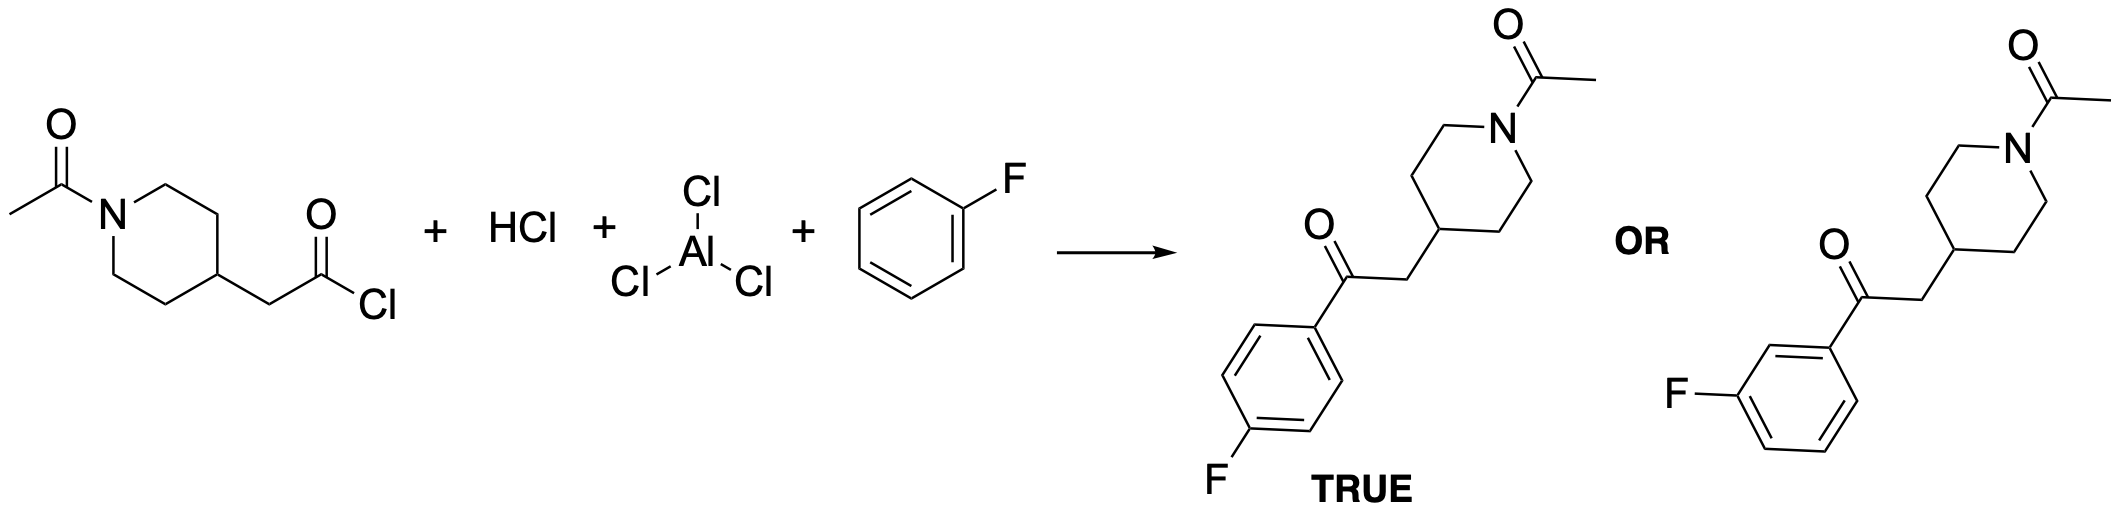
\includegraphics[width=0.9\textwidth]{Chapters/Transformer/Figs/sear.png}
% % \caption[FC]{Friedel-Crafts acylation reaction taken from the USPTO training set showing para selectivity.}
% % \label{fig:sear}
% % \end{figure}

% % \begin{figure}[htbp!] 
% % \centering    
% % 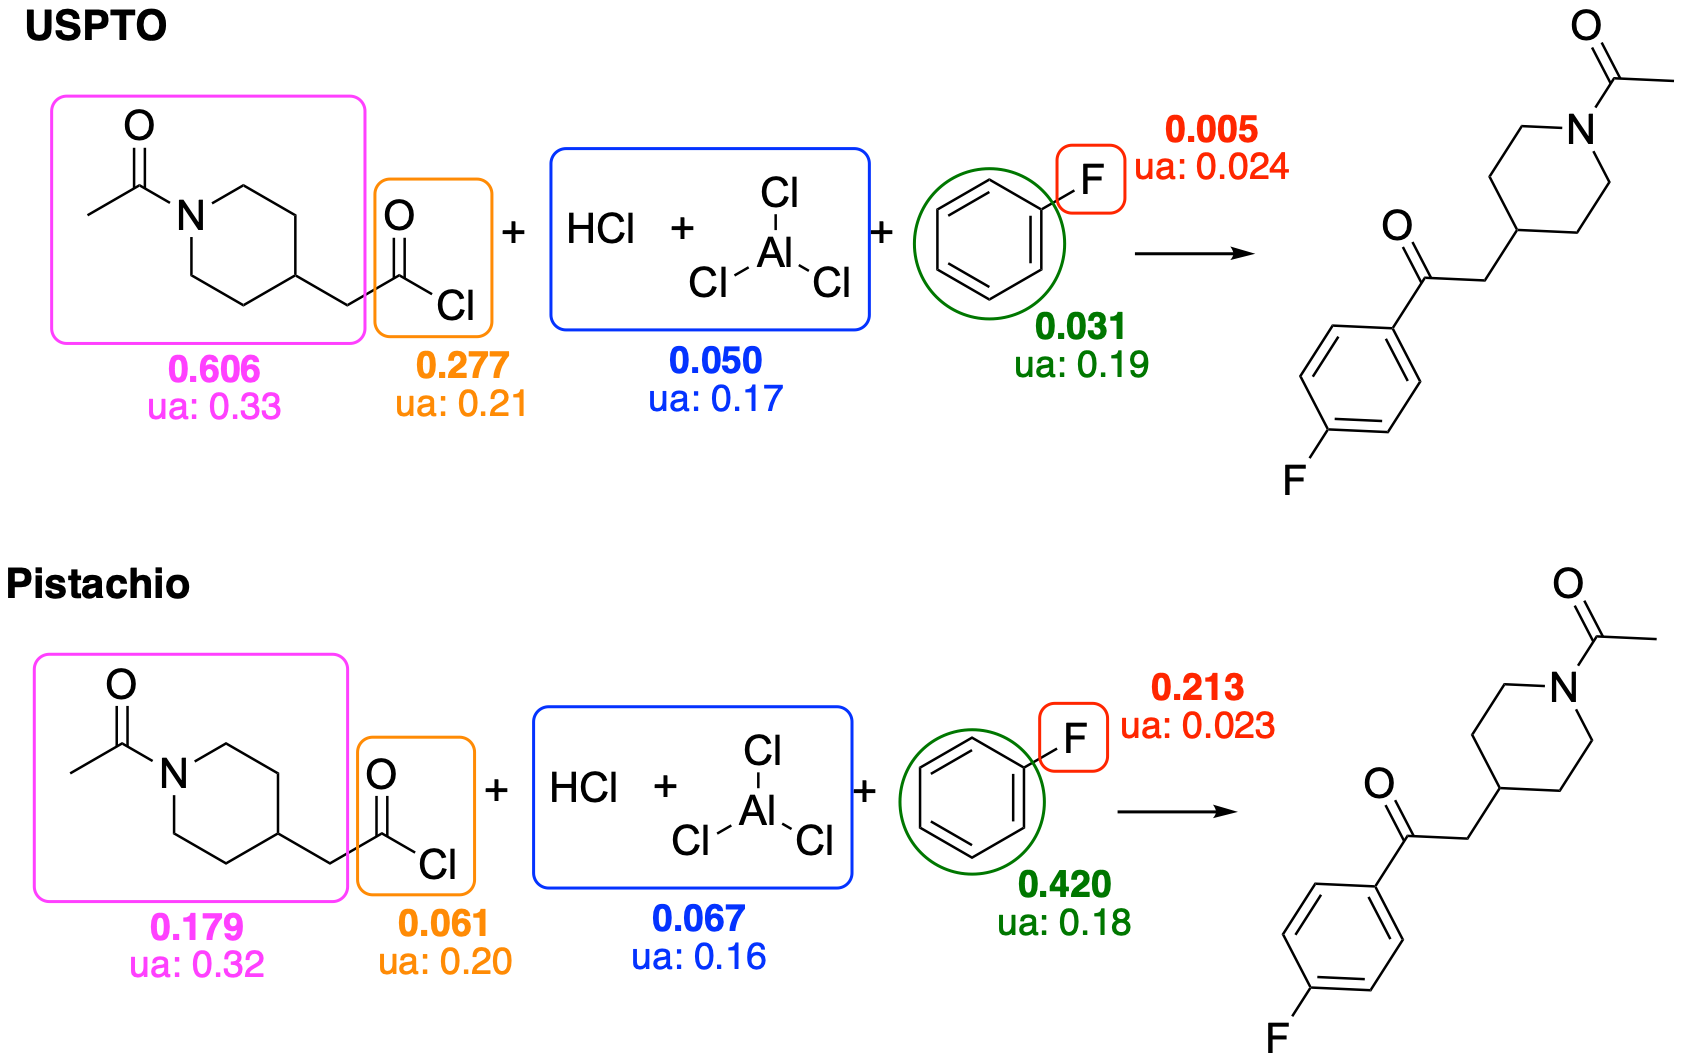
\includegraphics[width=0.8\textwidth]{Chapters/Transformer/Figs/sear_pred.png}
% % \caption[FC IG]{Both models predict the correct Friedel-Crafts acylation product but only the Pistachio model recognizes the importance of the -F atom in determining selectivity. The Integrated Gradients attributions are also shown along with the uniform attribution (ua) values. }
% % \label{fig:sear_pred}
% % \end{figure}

% % The predictions of the two models are shown in Fig~\ref{fig:sear_pred}. Both models predict the para selectivity correctly with confidence scores close to 1.0. When inspecting the IG attributions it can be seen that the USPTO model puts a very small weight on the Fluorine, only a fifth of the uniform attribution value. There is a large attribution given to the reagent though which does not affect the selectivity of this reaction at all. The attributions indicate that the USPTO transformer has not learnt the importance of F as the cause of para selectivity in these reactions. On the other hand the Pistachio transformer assigns a very high attribution value to F, suggesting that it has recognized the reason for the selectivity. 

% % Guided by the attributions we designed a number of adversarial examples where we have changed only the Fluorine part of the reactant-reagent input. This choice was motivated by the fact that according to the USPTO model the selectivity was driven by the reagents instead of the substituent on the benzene ring. If our interpretation is correct the model should keep predicting the para product even if a meta directing substituent is attached to the ring. The predictions of the models and the IG attributions of the meta directing groups are shown in Fig~\ref{fig:sear_adv}.

% % \begin{figure}[htbp!] 
% % \centering    
% % 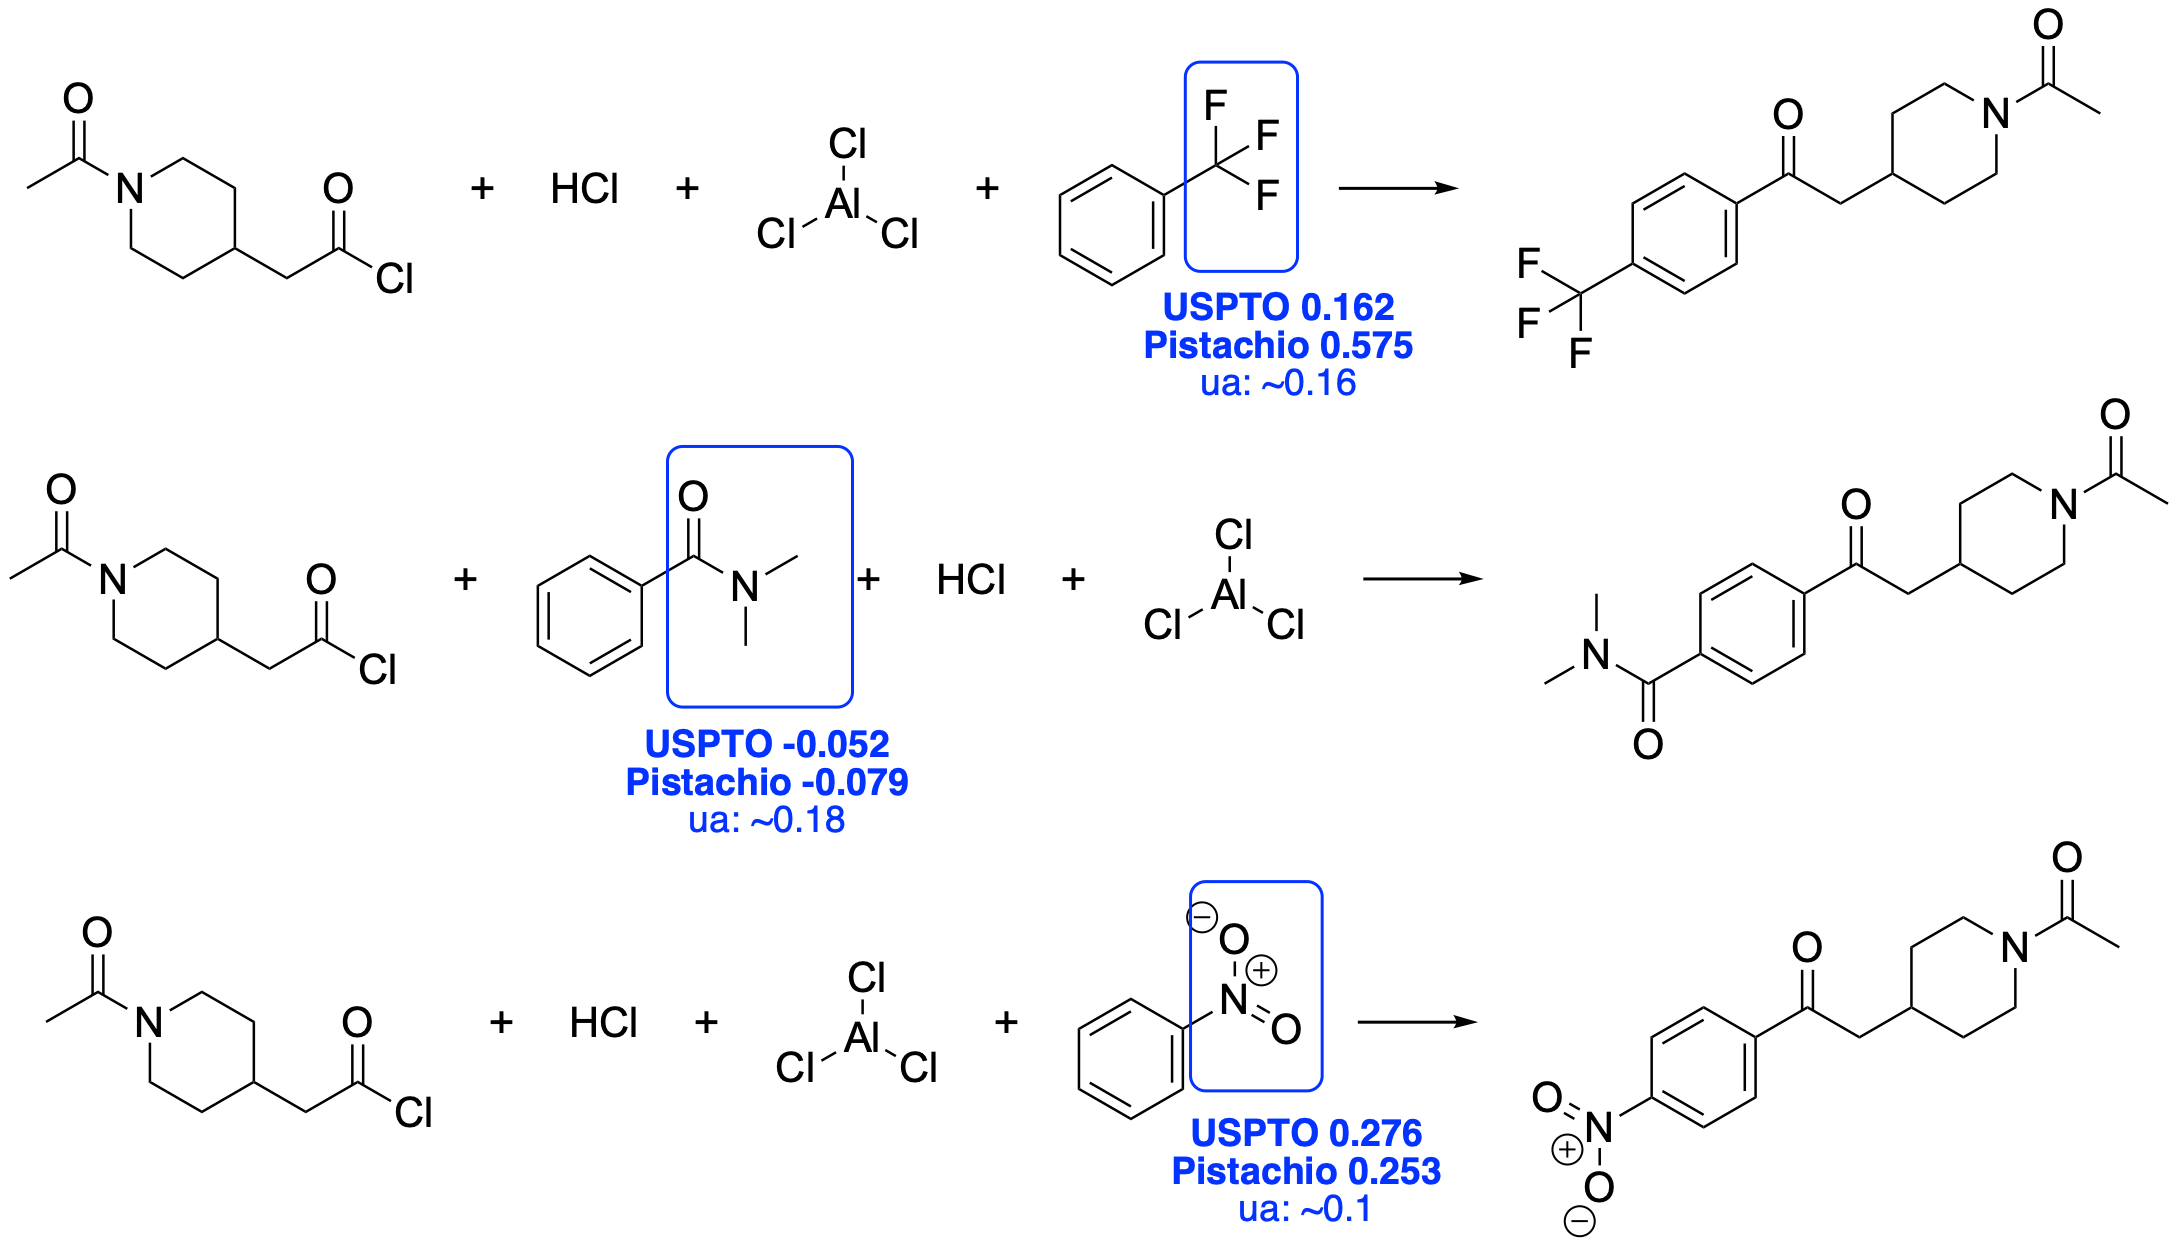
\includegraphics[width=1.0\textwidth]{Chapters/Transformer/Figs/sear_adv.png}
% % \caption[FC IG]{Adversarial examples designed using Fig~\ref{fig:sear_pred} reveal that both models can easily fail to predict the correct meta product. The uniform attribution (ua) values for the IGs are also shown. }
% % \label{fig:sear_adv}
% % \end{figure}

% % It can be seen that both transformer models fail in terms of predicting the meta directing effect of the substituents on the rings. In this case negative attributions favour the meta and positive the para product. There seems to be no correlation between the attribution values and the directing effect of the substituents, and even the Pistachio transformer is struggling with identifying the chemically important parts of the input. 

% % A suggestive observation is that in the second example the attributions on the meta directing group are negative, meaning that according to the models the amide group (correctly) favours the formation of the meta product. This agrees with chemical principles, but the model is still predicting the para to be the major product. We hypothesized that this might be due to biases in the training data, because if there are many more para substitution reactions than meta, the model could become biased towards predicting para substitutions even in the presence of meta directing groups. 

% % \begin{figure}[htbp!] 
% % \centering    
% % \includegraphics[width=0.65\textwidth]{Chapters/Transformer/Figs/sear_directing.png}
% % \caption[FC IG]{Counting the number Friedel-Crafts acylation reactions in the training sets with ortho, meta and para selectivities reveals an alarming bias -- the number of para reactions far outweigh those of meta or ortho reactions.}
% % \label{fig:sear_dir}
% % \end{figure}

% % To check if this hypothesis was correct we counted the number of ortho, meta and para Friedel-Crafts acylations in the training dataset using reaction templates. There was a large number of reactions matching multiple templates because often the benzene rings had multiple substituents on them. The results are summarized on Fig~\ref{fig:sear_dir}. 

% % The overall number of meta substitutions was 680 and 896 for the USPTO and Pistachio datasets respectively compared to the 952 and 1534 para substitutions. However, these numbers do not reveal the true extent of the bias as in our test case the benzene ring was only singly substituted. The number of reactions where there is only a single meta directing group on the ring is only 7 and 23 for the two datasets, which are extremely small numbers compared to those for a single para directing substituent which are 347 and 609, a ratio of 25-50 times.

% % This may result in the models not being able to learn meta directing substitution reactions because it can already achieve very high (~98\%) accuracy on the training set by always predicting the para product. The inclusion of further meta substitution reactions could considerably increase the models performance in real tasks. To confirm that the model would be able to learn the selectivities if the dataset was not biased, we probe the model with a synthetic dataset of para and meta Friedel-Crafts reactions in Sec.~\ref{subsec:synth_data}.

% % \subsection{Selective reduction of aldehydes and ketones}
% % Reduction of esters and aldehydes follow very well defined selectivity that is determined by the reducing agent. It is possible to reduce selectively an aldehyde or a ketone to alcohol in the presence of an ester. In this example the reduction of aldehydes using sodium-borohydride is examined \cite{Clayden2012}. If the Na is replaced by Li the reduction stops being selective to aldehydes and esters get reduced as well. The question is whether the models were able to learn the role of the cations in driving this subtle selectivity. An example reaction containing this selectivity is shown in Fig~\ref{fig:redu}.

% % \begin{figure}[htbp!] 
% % \centering    
% % \includegraphics[width=0.9\textwidth]{Chapters/Transformer/Figs/reduction.png}
% % \caption{An example of a reaction showing how NaBH\textsubscript{4} reduces the aldehydes selectively in the presence of an ester.}
% % \label{fig:redu}
% % \end{figure}

% % Both models are able to predict the product correctly with very high confidence (score > 0.95). In this case it is not immediately obvious what an interpretable attribution would be. One could argue that the selectivity is caused by Na\textsuperscript{+} because if we swap it to Li\textsuperscript{+} the other product would become the true product. The IG attributions on the \texttt{[Na+]} token are 0.013 and 0.017 for the USPTO and Pistachio models respectively, less than what the uniform attribution would be. This suggests that the models have not identified the importance of Na\textsuperscript{+} ion. 

% % To better understand the reliability of the predictions we attribute the reaction to the training data. For both models the most similar reactions (Fig~\ref{fig:redu_dat}) are BH\textsubscript{4} reductions of molecules containing both a ketone and an ester group. These examples suggest that both models have learnt this selectivity correctly, but they are not helping in understanding the role of the Na\textsuperscript{+}ion in the reaction.

% % \begin{figure}[htbp!] 
% % \centering    
% % \includegraphics[width=0.9\textwidth]{Chapters/Transformer/Figs/reduction_dat.png}
% % \caption{Data attribution to the reaction in Fig~\ref{fig:redu} suggests that both models have correctly learnt the selectivity of reduction.}
% % \label{fig:redu_dat}
% % \end{figure}

% % To investigate further if the models have learnt the importance of the cation in these reactions we designed an adversarial example where the only difference from the reaction on Fig~\ref{fig:redu} was the replacement of Na\textsuperscript{+} with Li\textsuperscript{+}. From Fig~\ref{fig:redu_adv} we see that the USPTO transformer keeps predicting the aldehyde being selectively reduced whereas the Pistachio model recognizes the change and predicts the correct product with both groups reduced. 

% % \begin{figure}[htbp!] 
% % \centering    
% % \includegraphics[width=0.9\textwidth]{Chapters/Transformer/Figs/redu_adv.png}
% % \caption{Adversarial example for the borohydride reduction in Fig~\ref{fig:redu} where the Na\textsuperscript{+} ion was replaced by Li\textsuperscript{+} ion. The USPTO model continues predicting the selective reduction of the aldehyde wrongly whereas the Pistachio model predicts the correct product -- the understanding of the models is reflecting in the IG attribution on the Li\textsuperscript{+} ion.}
% % \label{fig:redu_adv}
% % \end{figure}

% % To prove that one model was able to identify the importance of the cation and the other was not the IG attributions were generated and are shown in Fig~\ref{fig:redu_adv}. Here positive attributions favour the selective reduction, and the negative attributions favour the correct product. It is immediately obvious from the attributions that the USPTO model did not take into account the Li\textsuperscript{+} ion as it was given an attribution score that is an order of magnitude smaller than the uniform attribution value.

% % For the Pistachio model the probability score difference between the products was -0.21 and there was a lot of variation in attribution across different parts of the structure. The \texttt{[Li+]} token was given a very large negative attribution meaning that the model was strongly relying on it when making the correct prediction. Overall comparing the attributions it can be concluded that the USPTO model did not learn the chemistry of LiBH\textsubscript{4}, but the Pistachio one did. This can be due to the fact that the Pistachio model has seen more than 6 times more examples with this reagent. 

% % \subsection{Exploring the model with artificial data}
% % \label{subsec:synth_data}
% % One of the limitations of learning chemistry from patented and published reactions is that these reactions were designed by trained chemists who avoid transformations that have non-obvious selectivities. This makes it difficult for the models to infer the order of reactivity of functional groups. A further point is the effect of bias in the datasets on the models performance. To better understand these effect with full control over the experimental parameters, we have designed two artificial tasks where the training reaction data is generated using explicit SMARTS templates. 

% % In the first experiment we test whether the transformer model is able to learn selective chemistry if given enough data. We assembled a synthetic dataset of 90 000 reduction reactions. Carbon scaffolds were randomly selected from the ZINC database of drug-like molecules \cite{Irwin2005ZINCScreening}. To each scaffold we added an aldehyde group, an ester group, or both. Finally the 90 000 reactions, summarized in Table~\ref{table:red_datasets}, were obtained by applying one of three reduction templates shown in Fig~\ref{fig:redu_templates} to them. 

% % \begin{figure}[htbp!] 
% % \centering    
% % \includegraphics[width=0.6\textwidth]{Chapters/Transformer/Figs/redu_templates.png}
% % \caption[epoxide IG]{Three uniquely selective reduction templates are chosen to challenge the transformer's ability to learn selectivities if given enough data.}
% % \label{fig:redu_templates}
% % \end{figure}

% % \begin{table}[!h]
% % \caption{Number of reactions in the synthetic reduction datasets}
% % \centering
% % \label{table:red_datasets}
% % \begin{tabular}{m{0.17\textwidth}>{\centering}m{0.1\textwidth}>{\centering \arraybackslash}m{0.1\textwidth}>{\centering \arraybackslash}m{0.1\textwidth}}
% % \toprule
% %  \textbf{Subset} & \textbf{Aldehyde} & \textbf{Ester} & \textbf{Both}\\ 
% % \midrule
% % NaBH\textsubscript{4} & 20 000 & 0 & 10 000  \\
% % DIBAL & 0 & 20 000 & 10 000  \\
% % LiAlH\textsubscript{4} & 10 000 & 10 000 & 10 000  \\
% % \bottomrule
% % \end{tabular}
% % \end{table}

% % When training the transformer on this dataset we found that the only limiting factor in the performance of the model was its ability to reconstruct the sometimes tricky backbones of the molecules from the ZINC dataset. The selective chemistry was learnt (99\% top-1 accuracy) by the model in less than 10 000 steps. This shows that given sufficient data the model is able to learn selective transformations. To investigate how these findings are reflected in the IG attributions and verify that they are able to capture these empirical observations we generated the attributions for the reaction shown in Fig~\ref{fig:toy_attr}.

% % \begin{figure}[htbp!] 
% % \centering    
% % \includegraphics[width=1.00\textwidth]{Chapters/Transformer/Figs/toy_attr.png}
% % \caption{The model trained on artificial reduction data correctly attributes importance to the Al\textsuperscript{3+} ion.}
% % \label{fig:toy_attr}
% % \end{figure}

% % From the attributions we see that the model rightly gives high attribution to the Al\textsuperscript{3+} ion and small attribution to Li\textsuperscript{+}. This suggests that the model has learnt that it should only attend to one of the two tokens because they always appear together in the reactions. The H\textsuperscript{-} ions get a low attribution as expected. The attributions also verify that the model is finding the backbone part of the input very important, as reconstruction of the backbone is the most challenging aspect of making a correct prediction for this dataset of diverse backbones but restricted chemistry.
\chapter{Augmenting Nanomolar High-Throughput Screening with Machine Learning for Lead Optimisation}\label{ch:testing}

Typically, testing a drug candidate involves obtaining a pure sample of the molecule, and then mixing it in solution with the protein target under study to measure its bioactivity via an assay. While necessary for maximum accuracy, compound purification can be time-consuming and costly, particularly for chiral molecules. In collaboration with the London Lab at The Weizmann Institute of Science, we investigated whether we needed compound purification at all for training machine learning bioactivity models by using non-purified compound assays. Focusing on a particular scaffold synthesised with an amide coupling as the final step, we added the acid and amine reactants directly in solution with the protein to obtain an assay reading from the crude reaction mixture. By skipping the purification step, this allowed us to quickly screen a library of < 300 > amines with the same acid in high-throughput which we used to train RF and GP models. Leave-one-out validation on the training data correctly identified false negatives, and a prospective virtual screen of EnamineREAL with the trained models returned top hits with similar potency and better pharmacokinetic properties.

Machine learning (ML) has seen great advances over the past two decades in drug discovery and development, from protein-ligand interactions to novel scaffold generation to virtual screening of pharmacokinetic properties and toxicity.1-5 Generally, ML algorithms are tasked with prediction of specific target(s) with the endeavor that the faster predictions in silico will lead to faster pharmaceutical development. Hastening drug development is a key factor in reducing the overall cost of pharmaceutics, where it can reach up to \$2 billion to bring a compound to market.1 However, one overlooked area in this development cycle is ML applied as a filtering protocol for initial lead discovery, despite reports that ML methods often implicitly identify false positives and false negatives.6,7 Crude activity screening (assuming some level of introduction by Mihajlo is given previously) is a logical area to apply such techniques as noise and false hits/misses play a substantial role in obscuring valuable data. We hypothesized that combining two robust ML methodologies, Gaussian Processes (GPs) and Random Forests (RFs), could be used to identify hidden gems (false negatives) and overlooked molecules (low activity positives). Both GPs and RFs have been utilized in numerous chemoinformatics tasks, with several precedents in pharmaceutics development, making both ideal for predicting activity of novel compounds.8-12 Given the difference in approach to modeling for GPs and RFs, it was hypothesized that a combination of the two would lead to a highly robust framework; a compound predicted to have low activity from both a GP and a RF is likely to be inactive and likewise a compound with high predicted activity from both the GP and RF is likely potent.

Figure 1 - schematic

Thus, we separately trained a GP and RF on the crude inhibition data, identifying 5 compounds which had predicted activity from both the GP and RF but no crude activity. We suspected that these were false negatives and re-synthesized, purified, and re-tested them with full dose-response curves to obtain IC50 inhibition values. This revealed that one of them was active with IC50 = 0.113\uM (ASAP-0000204). (needs a nice sentence to round it off).

\begin{figure}
    \centering
             \includegraphics[width=0.45\textwidth]{Chapters/Crude/Figs/rf.pdf}
        \caption{Leave one out regression. }
        \label{fig:leave-one-out}
    \end{figure}
    
Looking forward, we test the ability of the trained models to extrapolate to novel compounds by prospectively screening an external library of amides. We virtually enumerate primary and secondary amine building blocks from Enamine with the same carboxylic acid substructure from the crude activity screening. This results in a library of ~62,800 amides which were scored by the trained GP and RF models, and we select the top 20 compounds with high predicted activity for both the GP and RF for synthesis and assaying to obtain IC50 values. Gratifyingly, the top 2 ML compounds showed promising average IC50 values of 0.0525\uM (ASAP-0000169) and 0.075\uM (ASAP-0000211), respectively. The top 2 most potent molecules based off of the crude inhibition values were compounds that, whilst active at IC50 = 0.034\uM (ASAP-0000221) and IC50 = 0.064\uM (ASAP-0000164), contained the toxic benzene-1,4-diamine motif that is generally avoided.13 The top 2 compounds without the aforementioned motif derived from only crude inhibition values had similar pure compound IC50 values to our framework's identified compounds, 0.046\uM (ASAP-0000155) and 0.064\uM (ASAP-0000225), respectively. This result highlights ML's ability to identify promising yet overlooked scaffolds without compromising potency. 

\begin{figure}
    \centering
             \includegraphics[width=0.45\textwidth]{Chapters/Crude/Figs/strip_plot.pdf}
        \caption{Plot of mean IC50 values.}
        \label{fig:strip}
    \end{figure}

Figure 4 - top 2 crude, false negative?

References:

1	Selvaraj, C., Chandra, I. \& Singh, S. K. Artificial intelligence and machine learning approaches for drug design: challenges and opportunities for the pharmaceutical industries. Molecular Diversity 26, 1893-1913, doi:10.1007/s11030-021-10326-z (2022).
2	Göller, A. H. et al. Bayer’s in silico ADMET platform: A journey of machine learning over the past two decades. Drug discovery today 25, 1702-1709 (2020).
3	Lavecchia, A. Machine-learning approaches in drug discovery: methods and applications. Drug Discovery Today 20, 318-331, doi:https://doi.org/10.1016/j.drudis.2014.10.012 (2015).
4	Lipinski, C. F., Maltarollo, V. G., Oliveira, P. R., Da Silva, A. B. \& Honorio, K. M. Advances and perspectives in applying deep learning for drug design and discovery. Frontiers in Robotics and AI 6, 108 (2019).
5	Vamathevan, J. et al. Applications of machine learning in drug discovery and development. Nature Reviews Drug Discovery 18, 463-477, doi:10.1038/s41573-019-0024-5 (2019).
6	Ardila, D. et al. End-to-end lung cancer screening with three-dimensional deep learning on low-dose chest computed tomography. Nature medicine 25, 954-961 (2019).
7	Ryu, J. Y., Lee, M. Y., Lee, J. H., Lee, B. H. \& Oh, K.-S. DeepHIT: a deep learning framework for prediction of hERG-induced cardiotoxicity. Bioinformatics 36, 3049-3055 (2020).
8	Jiménez-Luna, J., Grisoni, F. \& Schneider, G. Drug discovery with explainable artificial intelligence. Nature Machine Intelligence 2, 573-584, doi:10.1038/s42256-020-00236-4 (2020).
9	Reker, D. \& Schneider, G. Active-learning strategies in computer-assisted drug discovery. Drug discovery today 20, 458-465 (2015).
10	Kapsiani, S. \& Howlin, B. J. Random forest classification for predicting lifespan-extending chemical compounds. Scientific Reports 11, 13812, doi:10.1038/s41598-021-93070-6 (2021).
11	Svetnik, V. et al. Random Forest: A Classification and Regression Tool for Compound Classification and QSAR Modeling. Journal of Chemical Information and Computer Sciences 43, 1947-1958, doi:10.1021/ci034160g (2003).
12	Kang, B., Seok, C. \& Lee, J. Prediction of Molecular Electronic Transitions Using Random Forests. Journal of Chemical Information and Modeling 60, 5984-5994, doi:10.1021/acs.jcim.0c00698 (2020).
13	Kumar, M. S., Tamilarasan, R. \& Sreekanth, A. 4-Salicylideneamino-3-methyl-1,2,4-triazole-5-thione as a sensor for aniline recognition. Spectrochimica Acta Part A: Molecular and Biomolecular Spectroscopy 79, 370-375, doi:https://doi.org/10.1016/j.saa.2011.03.030 (2011).


\chapter{Outlook} \label{ch:outlook}

The research presented in this thesis explore ways in which data-driven approaches based on machine learning can be leveraged in the design-make-test cycle of drug discovery. In each of the three steps of `design', `make', and `test' we encounter the same underlying challenge, of grappling with the practical difficulties of a drug discovery campaign where we must make full use of the limited data available.

In Chapter \ref{ch:fresco} we looked at how to leverage fragment-protein structures from a crystallographic fragment screen to hit discovery in the absence of any bioactivity data. Using an unsupervised learning approach, we learn the geometric distribution of pharmacophores from the fragment-protein complexes, and use these to screen potential molecules for bioactivity. We showed that this approach outperforms docking on distinguishing active compounds from inactive ones on retrospective data. Further, we prospectively found novel hits for SARS-CoV-2 Mpro and the Mac1 domain of SARS-CoV-2 non-structural protein 3 by virtually screening a library of 1B molecules.

Chapter \ref{ch:ranking} takes us to the early stages of hit-to-lead molecular optimisation where bioactivity data is limited, noisy, and dominated by inactive molecules. We overcame this challenge with a learning-to-rank framework via an ML model that predicts whether a compound is more or less active than another. This approach allowed us to make use of inactive data and threshold the bioactivity differences above measurement noise, and validation on retrospective data for SARS-CoV-2 Mpro showed that we can outperform docking on ranking ligands. Combining this model with AI-based synthesis tools, we prospectively screened a library of 8.8M molecules to arrive at a potent compound with a novel scaffold.

While AI-based synthesis tools have already shown demonstrable success in accelerating the synthesis of new molecules, they are still prone to failure and suffer from a lack of transparency in their decision making due to their black-box nature. To address this, in Chapter \ref{ch:transformer} we showcased a workflow for quantitatively interpreting a state-of-the-art deep learning model for reaction prediction. By analysing chemically selective reactions, we showed examples of correct reasoning by the model, explain counterintuitive predictions, and identify Clever Hans predictions where the correct answer is reached for the wrong reason due to dataset bias.

In Chapter \ref{ch:testing} we explored how to accelerate testing procedures by applying machine learning on bioactivity data from nanomolar-scale high-thoughput chemistry. While this experimental technique greatly increases the number of molecules that can be tested, there is additional noise resulting from having to assay crude reaction mixtures instead of pure samples. Nevertheless, we showed that machine learning models trained on this data is able to cut through this noise and identify a false negative assay measurement, as well as prospectively screen a library of ~62K molecules to discover new SARS-CoV-2 Mpro inhibitors just as potent as those from the original assay.

\section{Directions for Future Research}

While we have explored some methods to accelerate the design-make-test cycle in this thesis, there is still much more work to be done to bring us closer to the dream of efficient and automated drug discovery. Below, we outline some of the most prominent directions for future research.

\subsection{Deploying and Extending ML-based Synthesis Tools}
Machine learning-based models for synthesis prediction have made significant strides in recent years, and are already sufficientily accurate to be deployed in industry for synthesis route design. However, translating these models into a practical tool that can be used by non-specialists is non-trivial. Connecting these models with commercial compound databases, updating models in response to changes in stock availability, and developing more user-friendly interfaces are fruitful engineering challenges for enabling more widespread adoption of these tools.

An intriguing extension of this idea is allowing a large language model (LLM) to access ML-based synthesis tools. Large language models, using the same architectures on which many ML synthesis tools are based on, have demonstrated incredible success in natural language processing as well as in understanding programming languages. An exciting use-case is to allow LLMs to make API calls to other software, meaning that one can abstract away complex programming tasks by just giving a natural language description of the task to the LLM. A recent example demonstrated how GPT-4, a powerful LLM, can perform molecular queries in the PubChem database, determine whether the molecule is purchasable, find a supplier that sells it and either purchase the compound or draft an email to a synthesis CRO to order. Integrating LLMs with ML-based synthesis tools, or augmenting LLMs by training them to understand SMILES and/or SMARTS, could extend such capabilities and facilitate complex user requests in synthesis planning.

In tandem with optimisng model deployment, continued improvement in the accuracy of synthesis predictions can be acheived in a number of ways. Novel model architectures that better reflect the underlying structure of chemical reaction data, both the graph nature of molecules as well as the correlations between chemical reactions from the same patent, could potentially improve the accuracy of synthesis predictions. The incorporation of proprietary reaction data from industry should also lead to improved performance, although there are difficulties in standardising data from electronic laboratory notebooks (ELNs) and there has been conflicting evidence regarding its usefulness. Finally, the creation of better benchmarks, likely incorporating disclosed industrial data, can help ensure that models are evaluated under realistic conditions, providing a more accurate and robust representation of their capabilities.

Last but not least, there is much room for improvment in the prediction of optimal reaction conditions and reaction yields, which are not currently handled by most ML-synthesis tools.  While existing models are effective at predicting the outcomes of small-scale chemical reactions, they may not be as accurate when it comes to predicting the behavior of reactions that must be scaled up for large-scale production. The inclusion of reaction yields and reaction conditions into ML synthesis models would allow for greater precision overall, and expand the scope of these models beyond small-scale reactions to bridge the gap between research and production.

\subsection{Addressing Data Scarcity}

A common challenge in drug discovery is the limited availability of data. While it is true that data scarcity is a persistent issue, it is also true that we are not making the most of the data that we do have. Existing datasets can be enhanced by utilizing them in more effective ways, and by designing models that take into account the unique structure inherent in the data. For example, imputation-based methods explicitly consider data sparsity, filling in missing data points with estimates derived from other data points which allows researchers to make use of incomplete datasets and exploit correlations between different endpoint measurements. Transfer learning approaches involve using knowledge gained from one dataset to inform the learning process in another domain, and there is a large scope for designing models that can utilise abundant noisy data to improve the prediction of low-data properties. By developing and utilizing models that are specifically designed for low-data regimes instead of merely adapting models performant in data-rich scenarios, we can make more accurate predictions and gain insights that would not be possible with traditional models.

Federated learning is another promising approach that can help overcome data scarcity by building models that can learn from proprietary data while maintaining data privacy. The pharmaceutical industry posesses orders of magnitude more data on experimental measurements than publicly available but that data is often proprietary and cannot be shared. Federated learning approaches allow us to pool data from multiple industrial partners while maintaining privacy and security of the underlying data, allowing us to build models more accurate than possible by any individual partner. A landmark example of this is the MELLODDY project, which brought together ten pharmaceutical companies and aggregated over 2.6+ billion confidential experimental data points for 21+ million different small molecules and 40+ thousand on-target and pharmacokinetics assays. The massive increase in collective training data, boosted predictive performance particularly for pharmacokinetics and safety panel assays. The methodology of this project is a strong foundation on which to build more powerful federated learning platforms in the future.

In parallel to maximising the use of existing data, there are also exciting opportunities to use machine learning methods to leverage noisy but high-throughput experimental techniques in drug discovery. One example of such a technique is DNA-encoded libraries, which enable the synthesis and screening of large numbers of compounds in a relatively short amount of time. While the resulting data may be noisy, the sheer volume of data generated makes it a valuable resource for model training and validation. There is a large scope for developing models that can leverage data from other under-utilised high-throughput techniques, from microfluidics platforms to high-throughput crystallography, to deliver novel insights in drug discovery.

\subsection{Integrate protein information into property prediction}
Accurate bioactivity prediction is still the primary bottleneck for computational drug design. Despite significant progress in recent years, predicting the efficacy of a drug candidate remains a complex challenge that involves a wide range of factors.

Recent advances in machine learning for protein bioinformatics offer promising new approaches to address this challenge. For example, researchers have developed deep learning models to predict protein structure and function, which can inform drug design strategies. By integrating these models and workflows with those for ML in chemistry and cheminformatics, we may be able to make significant breakthroughs in bioactivity prediction.

Expanding beyond bioactivity prediction, these models and workflows also have potential for predicting pharmacokinetics and toxicity properties, areas in which data scarcity and assay variability pose an even greater challenge than bioactivity prediction. By improving our ability to predict how a drug candidate will interact with biological systems, we can design more effective and safer drugs.

Finally, these advances may also have applications in predicting the molecular mechanisms of action, as well as identifying new drug targets. By combining insights from both chemical and biological data, we can gain a more comprehensive understanding of how drugs interact with the body at a molecular level, opening up new opportunities for drug discovery and design.

\subsection{Fully automated drug discovery}
Full automation of the drug discovery process is an ambitious goal that many researchers are working towards. The aim is to develop systems that can perform multiple iterations of the design-make-test process autonomously, with all decision-making handled by the system.

Recent developments in antibody design demonstrate the potential of this approach. Researchers have used machine learning to design and test thousands of potential antibody candidates, identifying promising new drug targets with unprecedented speed and accuracy.

However, achieving full automation of drug discovery will require integrating all of the models and workflows mentioned above, and developing new approaches to optimize decision-making and resource allocation. Reinforcement learning, in particular, could be the ultimate embodiment of this vision, enabling systems to learn from experience and continually improve their performance.

That said, the computational resources required for such an approach may be prohibitive in the near term, and significant technological breakthroughs will be required to make full automation of drug discovery a practical reality. Nonetheless, the potential benefits of such an approach are enormous, with the potential to transform the field of drug discovery and accelerate the pace of new drug development.


% ********************************** Back Matter *******************************
% Backmatter should be commented out, if you are using appendices after References
%\backmatter

% ********************************** Bibliography ******************************
\begin{spacing}{0.9}

% To use the conventional natbib style referencing
% Bibliography style previews: http://nodonn.tipido.net/bibstyle.php
% Reference styles: http://sites.stat.psu.edu/~surajit/present/bib.htm

\bibliographystyle{apalike}
% \bibliographystyle{unsrt} % Use for unsorted references  
% \bibliographystyle{plainnat} % use this to have URLs listed in References
\cleardoublepage
\bibliography{References/references} % Path to your References.bib file


% If you would like to use BibLaTeX for your references, pass `custombib' as
% an option in the document class. The location of 'reference.bib' should be
% specified in the preamble.tex file in the custombib section.
% Comment out the lines related to natbib above and uncomment the following line.

%\printbibliography[heading=bibintoc, title={References}]


\end{spacing}

% ********************************** Appendices ********************************

\begin{appendices} % Using appendices environment for more functionality

%!TEX root = ../thesis.tex
% ******************************* Thesis Appendix A ****************************
\chapter{Computational Details} \label{appendix:details}

\section{Docking against SARS-CoV-2} \label{appendix:docking}
All molecules synthesised by the COVID Moonshot Consortium were docked against structure x2908 reported by Diamond XChem \cite{Douangamath2020XChem}. We use the “Classic OEDocking” floe v0.7.2 as implemented in the Orion 2020.3.1 Academic Stack (OpenEye Scientific). Omega was used to enumerate conformations (and expand stereochemistry) with up to 500 conformations. FRED was used for docking in HYBRID mode using the x2908 bound ligand. The docked poses of the ligands were scored using the Chemgauss4 scoring function.

\section{Machine learning} \label{appendix:machine_learning}
\subsection{FRESCO} \label{appendix:fresco}
All data and code used for this work can be found in the GitHub repo \url{https://github.com/wjm41/frag-pcore-screen}. Supplementary figures and tables can be found in an accompanying file.

\subsection{Ranking model} \label{appendix:ranking}
Our training set, de novo design method and generated molecules are available on \url{https://github.com/wjm41/mpro-rank-gen}.

\subsection{Transformer model} \label{appendix:transformer}
The Molecular Transformer architecture used throughout this work is based on the model described in Schwaller et. al. \cite{Schwaller2019MolecularPrediction}. 

The model uses a 256 dimensional learnt embedding for each SMILES token. The encoder and the decoder are both made up of 4 standard transformer layers and dropout is applied with probability 0.1 \cite{Srivastava2014dropout}. For weight optimization the Adam optimizer is used and the model is trained for 500 000 steps. Checkpoints are saved every 10 000 steps and the final model is obtained by averaging the weights of the last 20 checkpoints for USPTO.

The model was implemented with OpenNMT-py package \cite{Klein2017} which makes use of the PyTorch framework \cite{paszke2019pytorch}. 

All code used for implementing the attribution tools for the Molecular Transformer, generating the artificial Friedel-Crafts dataset, and Tanimoto-splitting USPTO can be accessed in the GitHub repo \href{https://github.com/davkovacs/MTExplainer.git}{MTExplainer} \cite{Kovacs2020MolecularExplainer}. The USPTO dataset used to train the model \cite{Lowe2012, Jin2017}, as well as the Tanimoto similarity-based train/test splits of USPTO can also be found in the GitHub repo.
%!TEX root = ../thesis.tex
% ******************************* Thesis Appendix B ********************************

\chapter{Experimental Details} \label{appendix:experiments}

\section{Mpro assay} \label{appendix:mpro_assay}
The experimental procedure for measuring Mpro inhibition via Homogeneous Time Resolved Fluorescence (HTRF) assay is the same as that previously reported by COVID Moonshot\cite{Moonshot2022}, which is repeated below.

Dose response assays were performed in 12 point dilutions of 2-fold, typically beginning at 100\uM. Highly active compounds were repeated in a similar fashion at lower concentrations beginning at 10\uM or 1\uM. Reagents for Mpro assay were dispensed into the assay plate in 10$\mu$l volumes for a final volume of 20$\mu$L.

Final reaction concentrations were 20mM HEPES pH7.3, 1.0mM TCEP, 50mM NaCl, 0.01\% Tween-20, 10\% glycerol, 5nM Mpro, 37nM fluorogenic peptide sybstrate ([5-FAM]-AVLQSGFR-[Lys(Dabcyl)]-K-amide). Mpro was pre-incubated for 15 minutes at room temperature with compound before addition of substrate and ex/em filter set. Raw data was mapped and normalized to high (Protease with DMSO) and low (No Protease) controls using Genedata Screener software. Normalized data was then uploaded to CDD Vault (Collaborative Drug Discovery). Dose response curves were generated for IC50 using nonlinear regression with the Levenberg-Marquardt algorithm with minimum inhibition = 0\% and maximum inhibition = 100\%.

\section{OC43 antiviral assay} \label{appendix:oc43_assay}
A549 expressing H2B-mRuby were seeded in 384 well plates (4,000 cells per well) in DMEM+2\% FCS in a total volume of 30ul. One day later, 20ul of OC43 were added to the wells for a final MOI of 0.3. one hour after viral addition, the drug (or DMSO as control) was added to the cells. Drugs were added at a volume of 50nl, in a final dose range of 0.3-20mM. Cells were incubated at 33C, 5\% CO2 for 2 days, fixed with paraformaldehyde and stained for the presence of the viral nucleoprotein. Images were captured and quantified using the Incucyte machine and software. 3 biological repeated were performed.

\section{Model generated reaction schemes} \label{appendix:rxn_schemes}
\begin{figure}
    \centering
        \includegraphics[width=0.6\textwidth]{Chapters/Ranking/Figs/rxn_schemes_full.pdf}
        \caption{Model generated synthetic schemes for compounds $\mathbf{1}$-$\mathbf{5}$. The synthesis schemes generated by our model (grey) and the experimental schemes (black).}
        \label{fig:appendix_synthesis_schemes}
\end{figure}

\section{Mac1 assay} \label{appendix:mac1_assay}
Inhibition of SARS-CoV-2 nsp3-Mac1 (aa residues 206–379 of nsp3) was assessed by the displacement of an ADP-ribose conjugated biotin peptide from His6-tagged protein using a HTRF-technology-based screening assay which was performed as previously described \cite{Schuller2021Mac1Frag}. Compounds were dispensed into ProxiPlate-384 Plus (PerkinElmer) assay plates using an Echo 525 liquid handler (Labcyte). Binding assays were conducted in a final volume of 16 $\mu$l with 12.5 nM SARS-CoV-2 nsp3-Mac1 protein, 400 nM peptide ARTK(Bio)QTARK(Aoa-RADP)S (Cambridge Peptides), 1:20000 Anti-His6-Eu3+ cryptate (HTRF donor, PerkinElmer) and 1:125 Streptavidin-XL665 (HTRF acceptor, PerkinElmer) in assay buffer (25 mM HEPES pH 7.0, 20 mM NaCl, 0.05\% bovine serum albumin and 0.05\% Tween-20). Assay reagents were dispensed manually into plates using a multichannel pipette while macrodomain protein and peptide were first dispensed and incubated for 30 min at room temperature. This was followed by addition of the HTRF reagents and incubation at room temperature for 1 h. Fluorescence was measured using a PHERAstar microplate reader (BMG) using the HTRF module with dual emission protocol (A = excitation of 320 nm, emission of 665 nm, and B = excitation of 320 nm, emission of 620 nm). Raw data were processed to give an HTRF ratio (channel A/B $\times$ 10,000), which was used to generate IC50 curves. The IC50 values were determined by nonlinear regression using GraphPad Prism v.9 (GraphPad Software, CA, USA).

\section{Crystallographic screening on SARS-CoV-2 nsp3-Mac1} \label{appendix:mac1_crystallography}
Crystallographic screening of compounds was performed using Mac1 crystals grown in the P43 space group, following the previously described protocol (PMID: 33853786). Compounds synthesized by Enamine/WuXi were prepared in DMSO to 100 mM and were added to crystallization drops using an Echo 650 liquid handler (Labcyte) (PMID: 28291760). Crystals were soaked at either 10 or 20 mM for 2-4.5 hours, before being vitrified in liquid nitrogen using a Nanuq cryocooling device (Mitegen). Soak times and concentrations are listed in Table S1. Diffraction data were collected at beamlines 12-1 and 12-2 of the Stanford Synchrotron Radiation Lightsource (SSRL). The data collection strategy and statistics are listed in Table S1. Compound binding was detected using the PanDDA algorithm (PMID: 28436492) as described previously (PMID: 35794891). PanDDA was initially run using a background map calculated with 34 datasets collected from crystals soaked only in DMSO (annotated as dmso\_34 in Table S1). PanDDA was rerun with a background map calculated using two sets of 35 datasets where no compound binding was detected (annotated as either ssrl\_1 or ssrl\_2 in Table S1). This procedure led to the identification of an additional nine hits (Table S1). 

Compounds were modeled into PanDDA event maps using COOT (PMID: 20383002) with coordinates and restraints generated by phenix.elbow from SMILES strings (PMID: 19770504). Duplicate soaks were performed for most compounds: where the same compound was identified in multiple datasets, the highest occupancy compound was modeled. Both the compound-bound and compound-free coordinates were refined together as a multi-state model following the protocol described previously (PMID: 28436492). Compound occupancy was set based on the background density correction (BDC) value (PMID: 28436492). Refinement statistics are presented in Table S1. Coordinates and structure factor amplitudes have been deposited in the protein data bank (PDB) with the group deposition code G\_1002254. PanDDA input and output files have been uploaded to Zenodo (DOI: 10.5281/zenodo.7231822), and the raw diffraction images are available at https://proteindiffraction.org/.

\section{High-Throuhput Amide Coupling} \label{appendix:amide_coupling}
The amide library was made by reacting the carboxylic acid under the optimized reaction conditions (2 eq. amine; 2 eq. EDC; 2 eq. HOAt; 5 eq. DIPEA; DMSO; RT; 24h) with 300 amines (202 aromatics, 49 primary, and 49 secondary aliphatic amines). For library production, we used Echo LDV plates and an Echo 555 acoustic dispenser for liquid handling. Plate copies were made after diluting the reaction mixture with 4 μL DMSO. For yield estimation, 1 μL of the diluted library was transferred to an LC/MS-ready 384-well plate, followed by dilution with 20\% ACN in water to the final volume of 50 μL. The desired product was identified in 60\% of wells.

\end{appendices}

% *************************************** Index ********************************
\printthesisindex % If index is present

\end{document}
